%

\documentclass{book}
\usepackage[UTF8]{ctex}
\usepackage{fontspec}
%\usepackage{xeCJK}
\newCJKfontfamily\mincho{IPAexMincho}
\setCJKmainfont{SimSun}[ItalicFont=KaiTi, BoldFont=SimHei]

% SimSun
% STSong
% SimHei
% KaiTi
% DengXian

\def\topos{猫猫}
\def\nlab{$n$Lab}

\title{\textbf{\huge 盲人摸象}\\\emph{\topos{}理论讲义}}
\author{\emph{王进一}\\\href{我的邮箱}{jin12003@163.com}\\QQ 2917905525}
\date{2023 年夏至今\\~\\~此版本编译时间: \today{}~\\~\\这是一本正在施工的讲义. 目前我迫切需要读者的意见!
\\~\\
在非正式版本中, 我故意将 topos 译为 ``\topos{}''.
}

\usepackage{amsthm}
\usepackage{amsmath}
\usepackage{amssymb}
\usepackage{mathrsfs}
\usepackage{hyperref}

%\usepackage{wrapfig}

\usepackage{epigraph}

\usepackage{tikz}
\usetikzlibrary{cd}

\usepackage{enumerate}

\setcounter{secnumdepth}{1}
\setcounter{tocdepth}{1}

% 哲思

\newcommand{\philoquote}[2]{
\begin{center}
\begin{minipage}{0.7\linewidth}
{\quad\sffamily #1}\\
\begin{flushright}
\textsf{#2}
\end{flushright}
\end{minipage}
\end{center}~\\~\\
}

% 彩色方框, 参数的使用有点意思

\usepackage{tcolorbox}

\tcbuselibrary{breakable}

\newtcolorbox[
    auto counter,
    number within=section,
]{remark}[2][]{
    colback=blue!10!white,
    colframe=blue!10!white,
    coltitle=black,
    breakable,
    title={\textsf{注~\thetcbcounter} #2},
    #1
}

\def\examplecolor{pink!25!white}
\newtcolorbox[
    use counter from=remark,
    %number within=chapter,
]{example}[2][]{
    colback=\examplecolor,
    colframe=\examplecolor,
    coltitle=black,
    breakable,
    title={\textsf{例~\thetcbcounter} #2},
    #1
}
\newtcolorbox[
    use counter from=remark,
    %number within=chapter,
]{definition}[2][]{
    colback=red!10!white,
    colframe=red!10!white,
    coltitle=black,
    breakable,
    title={\textsf{定义~\thetcbcounter} #2},
    #1
}

\def\propcolor{green!20!white}
\newtcolorbox[
    use counter from=remark,
]{prop}[2][]{
    colback=\propcolor,
    colframe=\propcolor,
    coltitle=black,
    breakable,
    title={\textsf{命题~\thetcbcounter} #2},
    #1
}
\newtcolorbox[
    use counter from=remark,
]{propdef}[2][]{
    colback=orange!20!white,
    colframe=orange!20!white,
    coltitle=black,
    breakable,
    title={\textsf{命题-定义~\thetcbcounter} #2},
    #1
}

\newtcolorbox[
    auto counter,
    number within=chapter
]{exercise}[2][]{
    colback=gray!10!white,
    colframe=gray!10!white,
    coltitle=black,
    title={\textsf{习题~\alph{\thetcbcounter}} #2},
    #1
}
\newtcolorbox[
use counter from=remark,
]{axiom}[2][]{
	colback=cyan!30!white,
	colframe=cyan!30!white,
	coltitle=black,
	title={\textsf{公理~\thetcbcounter} #2},
	#1
}

% 分栏
\usepackage{multicol}

% 页眉与页脚样式
\usepackage{fancyhdr}
\pagestyle{fancy}
%\fancyhead{}
%\fancyhead[LE,RO]{\thepage}
\renewcommand{\chaptermark}[1]{\markboth{第\ \thechapter\ 章\ #1}{}}

% 页边距
\usepackage{geometry}
\geometry{
	b5paper,
	left=20mm,
	top=30mm,
}

% 参考文献
\usepackage{biblatex}
\addbibresource{Topos.bib}

% 章节样式
\usepackage{titlesec}
\titleformat{\chapter}{\huge\bfseries}{第\, \thechapter\, 章}{1em}{}

% 常用记号

\def\op{\text{op}} % 对偶范畴
\def\yo{\!\text{{\mincho よ}}} % 米田嵌入

\newcommand{\todo}[1]{{\color{red} [\textbf{未完成: #1}]}}

\begin{document}

\maketitle

\tableofcontents

\setcounter{chapter}{-1} % 这样下面一章就是第 0 章

% 第零章 前言
\chapter{前言}


每一个意象都是一个数学宇宙. 集合范畴 $\mathsf {Set}$ 是最简单和最重要的意象, 对应着 ``通常数学'' 的宇宙. 尽管一般意象可能有远比集合范畴丰富的结构, 其范畴论性质却与 $\mathsf {Set}$ 几乎相同. %意象的性质为几何学和逻辑学提供了良好的土壤: 几何学上, 每个意象中商空间, 纤维积, 映射空间等等构造有符合期望的性质; 逻辑学上, 每个意象都提供了一种语言以完全在范畴内部进行推理, 仿佛所处理的对象是普通集合一样. 对于熟悉的数学对象, 每一个意象都给我们一个新的视角; 一些关系在特定意象的语言中很简洁, 而在通常数学语言中则不然. 语言的重要性不言而喻.

拓扑空间 $X$ 上的层构成一个意象 $\operatorname{Sh}(X)$. 由此, 一般的意象可视为 ``广义空间'' 上的层范畴, 这种看法淡化范畴中的对象, 而将范畴当作一个整体. 意象还可视为一类直觉主义逻辑的语义. 意象理论的经典文献 \textit{Sketches of an Elephant} \cite{Elephant} 的开头列举了意象更多的解读方式, 正如盲人摸象一样.

本讲义参考了许多文献以及 nLab 上的无数条目. 讲义内容的编排原则大致是使初学者最易接受, 并且提供启发性的观点, 从而使人能更快入门去看更多的资料. 如果本讲义成功写下去的话, 或许能够改善这一领域缺少中文教材的现状.


\todo{重写前言}

\todo{解释本书不处理集合论问题 \cite{stacks-project}}

\newpage

~\vspace{4em}

\philoquote{
	Je vous souhaite le meilleur succès. Ce serait magnifique que vous puissiez étudier la théorie des topos de Grothendieck et travailler dans ce domaine. Travaillez beaucoup, soyez patient, ayez bon courage et vos efforts seront récompensés.
}{
	Laurent Lafforgue\footnotemark
}
\footnotetext{这是 Lafforgue 教授在一次讲座之后写给作者的话. ``祝愿你获得最大的成功. 你能够学习 Grothendieck 意象理论并在这个领域工作, 是一件美妙的事情. 努力学习, 保持耐心, 勇往直前, 你的努力将会得到回报.'' Lafforgue 教授是 Caramello 教授多年的合作者.}

\philoquote{Once you see at least one example and you do it yourself and you experience the kind of enlightenment it brings, you will be convinced forever.}{Olivia Caramello\footnotemark}
\footnotetext{这是 Caramello 教授在与作者的采访中关于 topos 理论的评论. Caramello 教授是意象理论和逻辑学专家.}

% TODO 详细介绍参考文献

% 第一章 范畴论

\chapter{\topos{}的范畴论性质}

\philoquote{
    The theory of abelian categories served as the
    ``right'' generalization for the category of abelian groups. So topoi serve for---no less---the category of sets.
}{Peter Freyd, \textit{Aspects of Topoi}}

范畴是一个广泛应用的概念, 然而它的结构比较单薄, 在一般的范畴中能做的事情十分有限. 为了让范畴更有用, 我们就要要求合适的性质. Lawvere 在范畴论的层面研究了这样一个问题: 集合范畴 $\mathsf {Set}$ 具有什么样的性质, 使得它能作为数学的基础. 他将这些性质提炼成为\topos{} (topos) 的概念.

本章的目的是展现集合范畴中的许多构造实际上具有范畴论上的一般性, 也为形式上统一这些构造的 ``\topos{}的内语言'' 埋下伏笔.

\section{范畴论基本概念}

\subsection{极限与余极限}

范畴中常见的极限如下.\footnote{我们假设读者对这些概念有一定的了解, 因此这里仅作一列举.}
\begin{itemize}
    \item \emph{乘积} (product) 是离散图 (若干个无关的对象) 的极限;
    \item \emph{等化子} (equalizer) 是形如 $\begin{tikzcd}[ampersand replacement=\&,sep=small]
	\bullet \& \bullet
	\arrow[shift left=1, from=1-1, to=1-2]
	\arrow[shift right=1, from=1-1, to=1-2]
\end{tikzcd}$ 的图的极限;
    \item \emph{拉回} (pullback) 是形如 $\begin{tikzcd}[ampersand replacement=\&,sep=small]
	\& \bullet \\
	\bullet \& \bullet
	\arrow[from=2-1, to=2-2]
	\arrow[from=1-2, to=2-2]
\end{tikzcd}$ 的图的极限;
    \item \emph{终对象}是空图的极限. 终对象也可视为 $0$ 个对象的积, 因此我们将终对象记作 $1$.
    终对象到另一对象 $c$ 的态射称为 $c$ 的\emph{整体元素} (global element)\footnote{这一称呼来自层的整体截面.}.
\end{itemize}

我们关注的一类极限是\emph{有限图} (有限个对象和有限个态射组成的图) 的极限, 称为\emph{有限极限}. (空图的极限也是一种有限极限.)

范畴中常见的余极限如下.
\begin{itemize}
    \item \emph{二元和}是形如 $\bullet\qquad \bullet$ 的图的余极限;
    \item \emph{余等化子} (coequalizer) 是形如 $\begin{tikzcd}[ampersand replacement=\&,sep=small]
	\bullet \& \bullet
	\arrow[shift left=1, from=1-1, to=1-2]
	\arrow[shift right=1, from=1-1, to=1-2]
\end{tikzcd}$ 的图的余极限;
    \item \emph{推出} (pushout) 是形如 $\begin{tikzcd}[ampersand replacement=\&,sep=small]
	\bullet \& \bullet \\
	\bullet \&
	\arrow[from=1-1, to=2-1]
	\arrow[from=1-1, to=1-2]
\end{tikzcd}$ 的图的余极限;
    \item \emph{始对象}是空图的余极限. 始对象也可视为 $0$ 个对象的和, 因此我们将始对象记作 $0$.
\end{itemize}

使用上面的某些 (余) 极限就可以表达出所有的有限 (余) 极限.

\begin{prop}
    [label={finite-limits-equivalent-condition}]
    {}
    \setlength{\tabcolsep}{12pt}
    \renewcommand{\arraystretch}{1.5}
    \begin{center}
    	\begin{tabular}{l|l}
    		对于范畴 $\mathsf C$, 如下条件等价: \quad & 对于范畴 $\mathsf C$, 如下条件等价: \\
    		(1) 存在有限极限\footnotemark; & (1) 存在有限余极限; \\
    		(2) 存在有限积与等化子; &  (2) 存在有限余积与余等化子;\\
    		(3) 存在终对象与拉回. & (3) 存在始对象与推出.
    	\end{tabular}
    \end{center}
\end{prop}

\footnotetext{``存在有限极限'' 是 ``存在所有的有限极限'' 的简便说法.}

\begin{proof}
    由对偶性, 我们只需证明左边的命题. 由定义, $(1)$ 蕴含 $(2)$ 和 $(3)$.
    
    $(2) \Rightarrow (1)$ 的证明. 设 $F \colon I \to\mathsf C, i\mapsto F_i$ 是任意有限图,
    考虑有限积
    $$
        P = \prod_{i} F_i,\quad
        Q = \prod_{i \to j} F_j
    $$
    (其中下标 $i\to j$ 取遍指标范畴 $I$ 的所有态射) 以及两个态射 $P \to Q$,
    一个是
    $(x_i)_{i} \mapsto (F_{i\to j}(x_i))_{i\to j}$,
    另一个是
    $(x_i)_{i} \mapsto (x_j)_{i\to j}$.
    两个态射的等化子即是极限 $\lim_{i} F_i$.
    注意态射 $P,Q$ 的定义仿佛使用了 ``集合'' 的语言,
    这可以视为一种形式的记号; 无论如何, 它很容易翻译为范畴语言.

    $(3) \Rightarrow (2)$ 的证明.
    到终对象的拉回给出了有限积,
    而对于两个态射 $f,g \colon X \to Y$, 如下拉回给出了等化子:
    % https://q.uiver.app/#q=WzAsNCxbMCwwLCJcXG9wZXJhdG9ybmFtZXtlcX0oZixnKSJdLFsxLDAsIlgiXSxbMCwxLCJYIl0sWzEsMSwiWSJdLFsxLDMsImYiXSxbMiwzLCJnIiwyXSxbMCwyXSxbMCwxXV0=
    \[\begin{tikzcd}[ampersand replacement=\&,column sep=small]
    	{\operatorname{eq}(f,g)} \& Y \\
    	X \& Y\times Y,
    	\arrow["\Delta", from=1-2, to=2-2]
    	\arrow["{(f,g)}"', from=2-1, to=2-2]
    	\arrow[from=1-1, to=2-1]
    	\arrow[from=1-1, to=1-2]
    \end{tikzcd}\]
    其中 $\Delta = (\operatorname{id}_Y,\operatorname{id}_Y) \colon Y\to Y\times Y$ 是\emph{对角线}.
\end{proof}

\subsection{指数对象与积闭范畴}

集合范畴中, 两个集合间的态射仍构成一个集合, 称为映射集合. 在某些范畴 $\mathsf C$ 中, 两个对象之间有一个 $\mathsf C$ 的对象充当了 ``映射集合'' 的角色, 称为\emph{指数对象} (exponential object).

\begin{definition}
    [label={exponential-object}]
    {(指数对象, 积闭范畴)}
    设范畴 $\mathsf C$ 具有有限积. 对固定的对象 $X$, 若存在函子 $(-)^X \colon \mathsf C \to \mathsf C$ 构成 $(-)\times X$ 的右伴随\footnotemark, 即有自然同构
    \begin{equation}
        \operatorname{Hom}_{\mathsf C}(Z,Y^X)  \simeq \operatorname{Hom}_{\mathsf C}(Z\times X,Y),
        \label{exponential-adjoint}
    \end{equation}
    则称 $X$ \emph{可作指数} (exponentiable), 称 $Y^X$ 为\emph{指数对象} (exponential object), 或称\emph{内蕴态射对象} (internal hom-object).
    
    若 $\mathsf C$ 的所有对象均可作指数, 则称 $\mathsf C$ 为\emph{积闭范畴} (cartesian closed category), 其中 ``闭'' 即指数对象的存在性.
\end{definition}

\footnotetext{指数对象可对一般的\emph{幺半范畴} (monoidal category) 定义, 这里我们只考虑所谓\emph{积幺半范畴} (cartesian monoidal category), 即以乘积定义的幺半范畴.}

指数对象在数学中随处可见.

\begin{example}
    {(紧开拓扑)}
    在拓扑空间范畴 $\mathsf {Top}$ 中, 一般的对象不一定可作指数, 但局部紧 Hausdorff 空间都是可作指数的.
    若 $X$ 是局部紧空间, $Y$ 是任意拓扑空间,
    指数对象 $Y^X$ 上的拓扑称为\emph{紧开拓扑} (compact-open topology),
    这个名字是因为它可由如下开集生成:
    对紧集 $K\subset X$ 与开集 $O\subset Y$,
    取 $X$ 到 $Y$ 所有满足 $f(K) \subset O$ 的映射构成的集合.
    
    拓扑学中, 人们常说 ``我们在一个方便的拓扑空间范畴中工作''\footnotemark,
    即要求所考虑的范畴包含我们感兴趣的空间, 且具有积闭等性质.
    一个比较方便的范畴是\emph{紧生成弱 Hausdorff 空间范畴} $\mathsf{CGWH}$. Johnstone \cite{Johnstone-OTT} 构造了一个方便的拓扑空间范畴, 且它是\topos{}.
\end{example}
\footnotetext{\url{https://ncatlab.org/nlab/show/convenient+category+of+topological+spaces}}

\begin{example}
    {(函子范畴)}
    两个范畴 $\mathsf C,\mathsf D$ 之间的函子构成一个范畴 $\mathsf {Fun}(\mathsf C,\mathsf D)$, 这是范畴的范畴 $\mathsf {Cat}$ 中的指数对象.
\end{example}

\begin{prop}
    {}
    对于积闭范畴, 指数对象实际上构成一个\emph{双函子} (也即乘积范畴出发的函子) $\mathsf C^{\op}\times\mathsf C \to \mathsf C$, $(X,Y)\mapsto Y^X$.
\end{prop}

    %指数对象的性质也可表述为函子 . 下面 (\ref{slice-category} 节) 还会介绍更多相关的性质.
    
    %另外, 即使范畴中没有乘积也可定义指数对象: 使用米田嵌入 $\yo \colon \mathsf C \to \mathsf {Fun}(\mathsf C^{\op},\mathsf {Set})$,
    %指数对象 $Y^X$ 是函子 $\yo(Y)^{\yo(X)}$ 的表示对象.

    

在集合范畴中, 给定一个映射 $f\colon X\to Y$ 与一个元素 $x\in X$, 我们可对 $f$ 在 $x$ 处取值得到 $Y$ 的元素 $f(x)$; 类似地, 在一个积闭范畴中我们有 $Y^X\times X$ 到 $Y$ 的一个 ``取值'' 映射.

\begin{definition}
    [label={evaluation-map}]
    {(取值映射)}
    在 (\ref{exponential-adjoint}) 中取 $Z=Y^X$, 那么 $\operatorname{id}_{Y^X}\in \operatorname{Hom}_{\mathsf C}(Y^X,Y^X)$ 在另一边对应的态射称作\emph{取值映射} (evaluation map) $\operatorname{ev}\colon Y^X\times X \to Y$. 换言之, 取值映射 $\operatorname{ev}\colon Y^X\times X \to Y$ 是伴随 $(-)\times X \dashv (-)^X$ 的余单位.
\end{definition}

指数对象有与数的乘方类似的规律.

\begin{prop}
	[label={exponential-law}]
	{(指数律)}
	在积闭范畴中, 对任意对象 $X,Y,Z$ 有
	$$
	(Z^{Y})^X\simeq Z^{Y\times X}.
	$$
\end{prop}

\begin{proof}
	由指数对象的性质, 有自然同构
	\begin{align*}
		\operatorname{Hom}(W,(Z^{Y})^X)
		&\simeq\operatorname{Hom}(W\times X,Z^Y)\\
		&\simeq\operatorname{Hom}(W\times X\times Y,Z)\simeq\operatorname{Hom}(W,Z^{Y\times X}).
	\end{align*}
	由米田引理, 结论得证.
\end{proof}

\begin{prop}
	[label={sum-exponential-product}]
	{}
	在有二元和的积闭范畴中, 对任意对象 $X,Y,Z$ 有
	$$
	Z^{X + Y}\simeq Z^X \times Z^Y.
	$$
\end{prop}

\begin{proof}
	略. 与命题 \ref{exponential-law} 的证明类似, 使用米田引理.
%	\begin{align*}
%		\operatorname{Hom}(W,Z^{X+Y})
%		&\simeq\operatorname{Hom}(W\times (X+Y),Z)\\
%		&\simeq\operatorname{Hom}(W\times X+W\times Y,Z)\\
%		&\simeq\operatorname{Hom}(W\times X,Z)+\operatorname{Hom}(W\times Y,Z)\\
%		&\simeq\operatorname{Hom}(W,Z^X)\times\operatorname{Hom}(W,Z^Y)\\
%		&\simeq\operatorname{Hom}(W,Z^X\times Z^Y).
%	\end{align*}
	其中要用到积闭范畴中的 ``分配律'' $$W\times (X+Y)\simeq W\times X+W\times Y,$$ 这是因为 $(-)\times W$ 作为 $(-)^W$ 的左伴随保持余极限 (命题 \ref{adjoints-preserve-limits}).
\end{proof}


\begin{prop}
	[label={product-exponential-product}]
	{}
	在积闭范畴中,
	$$
	(Z\times Y)^X\simeq Z^X\times Y^X.
	$$
\end{prop}

\begin{proof}
	这是因为 $(-)^X$ 作为 $(-)\times X$ 的右伴随保持极限 (命题 \ref{adjoints-preserve-limits}).
\end{proof}

\subsection{子对象分类子}

对于集合 $X$ 的子集 $U\subset X$,
定义其\emph{特征函数} (characteristic function) $\chi_U \colon X \to \{0,1\}$,
$$
\chi_U(x) = \begin{cases}
    \ 1, & x\in U,\\
    \ 0, & x\notin U.
\end{cases}
$$
(我们可将特征函数 $\chi_U(x)$ 视为 ``含一个变量 $x$ 的命题'', 当且仅当 $x\in U$ 时命题为真.)
如此, $X$ 的子集一一对应于 $X$ 到 $\{0,1\}$ 的映射.
这就是说, 集合 $\{0,1\}$ ``分类'' (classify) 了集合的子集.

\begin{definition}
    {(子对象)}
    在一般的范畴中, 我们称指向 $X$ 的单态射 $U \to X$ \emph{的同构类}为 $X$ 的\emph{子对象} (subobject), 其中单态射的同构是指形如
    % https://q.uiver.app/#q=WzAsMyxbMCwwLCJVIl0sWzAsMiwiXFx3aWRldGlsZGUgVSJdLFsxLDEsIlgiXSxbMCwyLCIiLDAseyJzdHlsZSI6eyJ0YWlsIjp7Im5hbWUiOiJob29rIiwic2lkZSI6InRvcCJ9fX1dLFsxLDIsIiIsMix7InN0eWxlIjp7InRhaWwiOnsibmFtZSI6Imhvb2siLCJzaWRlIjoiYm90dG9tIn19fV0sWzAsMSwiXFxzaW1lcSIsMix7Im9mZnNldCI6MX1dLFsxLDAsIiIsMSx7Im9mZnNldCI6MX1dXQ==
    $\begin{tikzcd}[ampersand replacement=\&,row sep=-1pt]
    	U \\
    	\& X \\
    	{\widetilde U}
    	\arrow[hook, from=1-1, to=2-2]
    	\arrow[hook', from=3-1, to=2-2]
    	\arrow["\simeq"', shift right=1, from=1-1, to=3-1]
    	\arrow[shift right=1, from=3-1, to=1-1]
    \end{tikzcd}$
    的交换图.
\end{definition}



范畴 $\mathsf C$ 中对象 $X$ 的子对象构成一偏序集 $\operatorname{Sub}_{\mathsf C}(X)$, 其序关系为 ``包含'' 关系. 若子对象 $U\hookrightarrow X$ 作为嵌入映射可分解为 $U\hookrightarrow V \hookrightarrow X$, 则称 $U$ 包含于 $V$.
%这个偏序集作为范畴, 其中的乘积为子对象的\emph{交}.

在范畴 $\mathsf C$ 具有拉回时, 子对象集合有函子性.

\begin{definition}{(子对象函子)}
    假设范畴 $\mathsf C$ 具有拉回. 定义\emph{子对象函子}
    $$\operatorname{Sub}_{\mathsf C} \colon \mathsf C^{\op} \to \mathsf {Set},$$
    将对象 $X$ 对应到其子对象的集合,
    态射对应到子对象的拉回.
\end{definition}

上述定义的合法性来自如下命题.

\begin{prop}{}
    在任何范畴中拉回保持子对象; 即对任意态射 $f \colon X \to Y$ 以及子对象 $i \colon V \to Y$, 只要存在拉回 $U = X\times_{Y} V$, 就有 $j=f^* i\colon U\to X$ 是 $X$ 的子对象.
    % https://q.uiver.app/#q=WzAsNCxbMCwxLCJYIl0sWzEsMSwiWSJdLFsxLDAsIlYiXSxbMCwwLCJVIl0sWzAsMSwiZiIsMl0sWzMsMCwiaiIsMix7InN0eWxlIjp7InRhaWwiOnsibmFtZSI6Imhvb2siLCJzaWRlIjoiYm90dG9tIn19fV0sWzMsMiwicCJdLFsyLDEsImkiLDAseyJzdHlsZSI6eyJ0YWlsIjp7Im5hbWUiOiJob29rIiwic2lkZSI6ImJvdHRvbSJ9fX1dXQ==
\[\begin{tikzcd}[ampersand replacement=\&]
	U \& V \\
	X \& Y
	\arrow["f"', from=2-1, to=2-2]
	\arrow["j"', hook', from=1-1, to=2-1]
	\arrow["p", from=1-1, to=1-2]
	\arrow["i", hook', from=1-2, to=2-2]
\end{tikzcd}\]
\end{prop}
\begin{proof}
    设 $j$ 余等化 $\alpha,\beta \colon Z \to U$.% 满足 $j \alpha = j \beta$.
    那么 $fj=ip$ 也余等化 $\alpha,\beta$.
    由 $i$ 为单态射, 知 $p$ 余等化 $\alpha,\beta$.
    由拉回的性质, 知 $\alpha = \beta$.
    这说明 $j$ 为单射.
\end{proof}


\begin{definition}[label={Subobject-classifier-definition}]{(子对象分类子)}
    设范畴 $\mathsf C$ 存在拉回. 若子对象函子 $\operatorname{Sub} \colon \mathsf C^{\op} \to \mathsf {Set}$ 可表, 即存在对象 $\Omega$ 使得有自然同构
    $$
    \operatorname{Sub}_{\mathsf C}(X) \simeq \operatorname{Hom}_{\mathsf C}(X,\Omega),
    $$
    则称 $\Omega$ 为 $\mathsf C$ 的\emph{子对象分类子} (subobject classifier).
\end{definition}

子对象分类子还有如下的等价定义.

\begin{definition}[label={Subobject-classifier-definition-alternative}]{(子对象分类子, 等价定义)}
    设范畴 $\mathsf C$ 存在拉回以及终对象 $1$. 若存在满足如下条件的对象 $\Omega$ 以及单射 $\top \colon 1 \to \Omega$, 则称其为 $\mathsf C$ 的\emph{子对象分类子} (subobject classifier): 对任意单射 (子对象) $U \to X$ 存在唯一的\emph{特征函数} (characteristic map) $\chi_U \colon X \to \Omega$ 使得下图为拉回.
    % https://q.uiver.app/#q=WzAsNCxbMCwwLCJVIl0sWzAsMSwiWCJdLFsxLDAsIjEiXSxbMSwxLCJcXE9tZWdhIl0sWzEsMywiXFxjaGlfVSIsMl0sWzAsMSwiIiwwLHsic3R5bGUiOnsidGFpbCI6eyJuYW1lIjoiaG9vayIsInNpZGUiOiJib3R0b20ifX19XSxbMiwzLCJcXHRvcCIsMCx7InN0eWxlIjp7InRhaWwiOnsibmFtZSI6Imhvb2siLCJzaWRlIjoiYm90dG9tIn19fV0sWzAsMl1d
    \[\begin{tikzcd}[ampersand replacement=\&]
    	U \& 1 \\
    	X \& \Omega
    	\arrow["{\chi_U}"', from=2-1, to=2-2]
    	\arrow[hook', from=1-1, to=2-1]
    	\arrow["\top", hook', from=1-2, to=2-2]
    	\arrow[from=1-1, to=1-2]
    \end{tikzcd}\]
    我们也称 $\top \colon 1 \to \Omega$ 为\emph{万有子对象} (universal subobject).
\end{definition}

有了子对象分类子, 子对象等同于到 $\Omega$ 的态射, 从而子对象的拉回不过是到 $\Omega$ 的态射的复合.
% https://q.uiver.app/#q=WzAsNixbMCwxLCJYIl0sWzEsMSwiWSJdLFsyLDEsIlxcT21lZ2EiXSxbMiwwLCIxIl0sWzEsMCwiViJdLFswLDAsImZeKlYiXSxbNSwwLCIiLDAseyJzdHlsZSI6eyJ0YWlsIjp7Im5hbWUiOiJob29rIiwic2lkZSI6ImJvdHRvbSJ9fX1dLFswLDEsImYiLDJdLFsxLDJdLFs1LDRdLFs0LDNdLFszLDIsIlxcdG9wIl0sWzQsMSwiIiwxLHsic3R5bGUiOnsidGFpbCI6eyJuYW1lIjoiaG9vayIsInNpZGUiOiJib3R0b20ifX19XV0=
\[\begin{tikzcd}[ampersand replacement=\&]
	{f^*V} \& V \& 1 \\
	X \& Y \& \Omega
	\arrow[hook', from=1-1, to=2-1]
	\arrow["f"', from=2-1, to=2-2]
	\arrow[from=2-2, to=2-3]
	\arrow[from=1-1, to=1-2]
	\arrow[from=1-2, to=1-3]
	\arrow["\top", from=1-3, to=2-3]
	\arrow[hook', from=1-2, to=2-2]
\end{tikzcd}\]

\begin{remark}{}
    ``万有子对象'' 中的 ``万有'' 与拓扑学中 ``万有 $G$-主丛'' 中 ``万有'' 的含义相同.

    上述定义中 ``$1$ 是终对象'' 的要求可不用提, 因为它蕴含于后面的泛性质中: 对任何对象 $X$ 考虑子对象 $\operatorname{id}\colon X \to X$, 在拉回图
    % https://q.uiver.app/#q=WzAsNCxbMCwwLCJYIl0sWzAsMSwiWCJdLFsxLDEsIlxcT21lZ2EiXSxbMSwwLCJcXHdpZGV0aWxkZSAxIl0sWzAsMSwiXFxvcGVyYXRvcm5hbWV7aWR9IiwyXSxbMCwzLCJcXGFscGhhIl0sWzEsMiwiXFxjaGkiLDJdLFszLDIsIlxcdG9wIl1d
    $\begin{tikzcd}[ampersand replacement=\&,sep=small]
	X \& {\widetilde 1} \\
	X \& \Omega
	\arrow["{\operatorname{id}}"', from=1-1, to=2-1]
	\arrow["\alpha", from=1-1, to=1-2]
	\arrow["\chi"', from=2-1, to=2-2]
	\arrow["\top", from=1-2, to=2-2]
    \end{tikzcd}$
    中, 由 $\chi$ 的唯一性以及 $\top$ 是单射可得到 $\alpha$ 的唯一性, 这说明 $\widetilde 1$ 就是\makebox{终对象 $1$.}
    
    符号 $\top$ (\LaTeX 代码: \verb|\top|) 读作 ``真'', 后面也将用到另一个元素 $\bot\colon 1\to\Omega$ (\verb|\bot|), 读作 ``假''. 一般地, 态射 $1\to\Omega$ 称为\emph{真值} (truth value).
\end{remark}

现在证明子对象分类器两种定义的等价性. 假设第一种定义 (\ref{Subobject-classifier-definition}) 中的对象 $\Omega$ 存在, 我们需要给出第二种定义 (\ref{Subobject-classifier-definition-alternative}) 所要求的单射 $\top\colon 1 \to \Omega$.

考虑 $\Omega$ 到自身的恒等映射 $\operatorname{id}\colon \Omega \to \Omega$, 它在同构 $\operatorname{Sub}(\Omega) \simeq \operatorname{Hom}(\Omega,\Omega)$ 下对应一个子对象 $\widetilde \top \colon \widetilde 1 \to \Omega$.

对任意子对象 $U\to X$, 由交换图
\[\begin{tikzcd}[ampersand replacement=\&]
	{\widetilde 1} \& {\operatorname{Sub}(\Omega)} \& {\operatorname{Hom}(\Omega,\Omega)} \& {\operatorname{id}_{\Omega}} \\
	U \& {\operatorname{Sub}(X)} \& {\operatorname{Hom}(X,\Omega)} \& {\chi_U}
	\arrow["\ni"{marking}, draw=none, from=1-4, to=1-3]
	\arrow["\simeq", <->, from=1-2, to=1-3]
	\arrow["\simeq"', <->, from=2-2, to=2-3]
	\arrow["\in"{marking}, draw=none, from=1-1, to=1-2]
	\arrow["\in"{marking}, draw=none, from=2-1, to=2-2]
	\arrow["\ni"{marking}, draw=none, from=2-4, to=2-3]
	\arrow["{\text{沿 $\chi_U$ 拉回}}"', from=1-2, to=2-2]
	\arrow["{\text{复合 $\chi_U$}}", from=1-3, to=2-3]
\end{tikzcd}\]
我们得到
% https://q.uiver.app/#q=WzAsNCxbMCwwLCJVIl0sWzAsMSwiWCJdLFsxLDAsIlxcd2lkZXRpbGRlIDEiXSxbMSwxLCJcXE9tZWdhIl0sWzAsMSwiIiwwLHsic3R5bGUiOnsidGFpbCI6eyJuYW1lIjoiaG9vayIsInNpZGUiOiJib3R0b20ifX19XSxbMiwzLCJ0IiwwLHsic3R5bGUiOnsidGFpbCI6eyJuYW1lIjoiaG9vayIsInNpZGUiOiJib3R0b20ifX19XSxbMSwzLCJcXGNoaV9VIiwyXSxbMCwyXV0=
$\begin{tikzcd}[ampersand replacement=\&,sep=small]
	U \& {\widetilde 1} \\
	X \& \Omega
	\arrow[hook', from=1-1, to=2-1]
	\arrow["{\widetilde \top}", hook', from=1-2, to=2-2]
	\arrow["{\chi_U}"', from=2-1, to=2-2]
	\arrow[from=1-1, to=1-2]
\end{tikzcd}$
是一个拉回. 这说明 $\widetilde \top$ 就是 $\top$.

%\begin{remark}{}
%    考虑 $1$ 的子对象 $\operatorname{id}\colon 1 \to 1$, 它在同构 $\operatorname{Sub}(1) \simeq \operatorname{Hom}(1,\Omega)$ 下对应特征函数 $\chi \colon 1 \to \Omega$. 是否这个函数也等于 $\top$?
%\end{remark}

下面介绍一些子对象的例子.

\begin{example}
    [label={self-as-subobject}]
    {(自身)}
    每个对象 $X$ 都是自身的子对象; 严格地说, $\operatorname{id}_X \colon X \to X$ 是一个子对象.
    它的特征函数是 $\top_X \colon X \to 1 \overset{\top}{\to}\Omega$.
    读者可验证下图确实是一个拉回:
    % https://q.uiver.app/#q=WzAsNCxbMCwwLCJYIl0sWzAsMSwiWCJdLFsxLDEsIlxcT21lZ2EiXSxbMSwwLCIxIl0sWzAsMSwiXFxvcGVyYXRvcm5hbWV7aWR9X1giLDJdLFswLDNdLFszLDIsIlxcdG9wIl0sWzEsMiwiXFx0b3BfWCIsMl1d
\[\begin{tikzcd}[ampersand replacement=\&]
	X \& 1 \\
	X \& \Omega.
	\arrow["{\operatorname{id}_X}"', from=1-1, to=2-1]
	\arrow[from=1-1, to=1-2]
	\arrow["\top", from=1-2, to=2-2]
	\arrow["{\top_X}"', from=2-1, to=2-2]
\end{tikzcd}\]
\end{example}

\begin{example}
	{(整体元素)}
	任何整体元素 $1\to X$ 是子对象.
\end{example}

\begin{example}
    [label={diagonal}]
    {(对角线)}
    假设二元积存在, 那么对任意对象 $X$, \emph{对角线映射} $\Delta \colon X \to X\times X$ 是一个子对象 (因为它复合任意一个投影映射得到 $\operatorname{id}_X$).
    % https://q.uiver.app/#q=WzAsNCxbMCwwLCJYIl0sWzAsMSwiWFxcdGltZXMgWCJdLFsxLDEsIlxcT21lZ2EiXSxbMSwwLCIxIl0sWzAsMSwiXFxEZWx0YSIsMl0sWzAsM10sWzMsMiwiXFx0b3AiXSxbMSwyLCJcXGNoaV9cXERlbHRhIiwyXV0=
\[\begin{tikzcd}[ampersand replacement=\&]
	X \& 1 \\
	{X\times X} \& \Omega
	\arrow["\Delta"', from=1-1, to=2-1]
	\arrow[from=1-1, to=1-2]
	\arrow["\top", from=1-2, to=2-2]
	\arrow["{\chi_\Delta}"', from=2-1, to=2-2]
\end{tikzcd}\]
    我们将它的特征函数 $\chi_{\Delta}$ 记为 ``Kronecker $\delta$ 函数'' $\delta_X \colon X \times X \to \Omega$, 表示 $X$ 上的\emph{相等}关系.
\end{example}

\begin{example}
	[label={singleton}]
	{(单元集)}
	``Kronecker $\delta$ 函数'' $\delta_X \colon X\times X\to \Omega$ 对应的态射 $\{-\}_X\colon X \to \Omega^X$ 称为\emph{单元集映射} (singleton map), 在集合范畴中它将 $X$ 的元素变为 $X$ 的单元子集.
	
	由下面的命题, $\{-\}_X$ 为单射, 从而它给出了 $PX$ 的一个子对象, 即 ``$X$ 的单元子集的集合''. 其特征函数
	$$
	\sigma_X := \chi_{\{-\}_X}\colon PX \to \Omega
	$$
	在直观上表示 $X$ 的一个子集是否是单元集.
\end{example}

\begin{prop}
	{(单元集映射是单射)}
	对任意对象 $X$, 单元集映射 $\{-\}_X\colon X \to \Omega^X$ 是单射.
\end{prop}

\begin{proof}
	对任意两个态射 $x,x'\colon U\to X$, 假设 $\{-\}_X\circ x = \{-\}_X\circ x'\colon U\to \Omega^X$, 那么由 $\delta_X$ 的定义有
	$$
	\delta_X(x\times 1) = \delta_X(x'\times 1) \colon U\times X \to \Omega.
	$$
	考虑下图,
	% https://q.uiver.app/#q=WzAsNixbMCwxLCJVXFx0aW1lcyBYIl0sWzAsMCwiVSJdLFsxLDEsIlhcXHRpbWVzIFgiXSxbMSwwLCJYIl0sWzIsMCwiMSJdLFsyLDEsIlxcT21lZ2EiXSxbMSwwLCIoMSx4KSIsMl0sWzAsMiwieFxcdGltZXMxIiwyXSxbMywyLCJcXERlbHRhIl0sWzEsMywieCJdLFszLDRdLFsyLDUsIlxcZGVsdGFfeCIsMl0sWzQsNV1d
	\[\begin{tikzcd}[ampersand replacement=\&]
		U \& X \& 1 \\
		{U\times X} \& {X\times X} \& \Omega
		\arrow["{(1,x)}"', from=1-1, to=2-1]
		\arrow["x\times1"', from=2-1, to=2-2]
		\arrow["\Delta", from=1-2, to=2-2]
		\arrow["x", from=1-1, to=1-2]
		\arrow[from=1-2, to=1-3]
		\arrow["{\delta_x}"', from=2-2, to=2-3]
		\arrow[from=1-3, to=2-3]
	\end{tikzcd}\]
	两个小方形均为拉回, 从而长方形为拉回.
	因此左边的竖直箭头 $(1,x)\colon U \to U\times X$ 是一个子对象 (函数 $x$ 的 ``图像''), 其特征函数为 $\delta_X(x\times 1)$.
	对于 $x'$ 有同样的拉回图, 故 $(1,x)$ 与 $(1,x')$ 是相同的子对象. 由子对象相同的定义,
	存在自同构 $h\colon U\to U$ 使得 $(1,x)\circ h = (1,x')$,
	即 $h=1, xh=x'$, 这说明 $x=x'$.
\end{proof}

\begin{example}
    [label={equalizer-as-subobject}]
    {(等化子)}
    假设二元积存在, 那么等化子可表示为一个子对象: 态射 $f,g \colon X \to Y$ 的等化子是态射
$$
X \overset{(f,g)}{\longrightarrow} Y\times Y \overset{\chi_{\Delta}}{\longrightarrow} \Omega
$$
对应的子对象. 对比命题 \ref{finite-limits-equivalent-condition} $(3) \Rightarrow (2)$ 的证明.
\end{example}

\begin{example}
    [label={membership-relation}]
    {(成员关系)}
    取值映射 (见定义 \ref{evaluation-map}) $\Omega^X \times X \to \Omega$ 对应的子对象是\emph{成员关系} (membership relation) $\in_X \hookrightarrow \Omega^X \times X = P(X) \times X$.
\end{example}

\begin{remark}
    {(子对象, 谓词与广义元素)}
    集合的函数 $X \to \{\top,\bot\}$ 可视为定义在 $X$ (的元素) 上的一个\emph{谓词}, 也即输入 $X$ 的元素 $x$, 输出 $x$ 是否满足某个命题. %在第三章我们会详细介绍这种观点, 这里仅提供感性的认识:
    $X$ 自身作为子对象, 对应谓词 $\top$ (恒真);
    对角线 $\Delta \colon  X\to X\times X$ 对应谓词 ``$x=y$'';
    等化子 $\operatorname{eq}(f,g) \to X$ 对应谓词 ``$f(x)=g(x)$''.

    态射 $A \to X$ 可视为 $X$ 的\emph{广义元素}. 设 $X \to \Omega$ 是谓词, 那么复合 $A \to X \to \Omega$ 可视为 $\Omega$ 的广义元素, 表示 ``广义元素 $A \to X$ 满足谓词 $X\to\Omega$''.
\end{remark}

\subsection{幂对象}

集合 $X$ 的幂集 (power set) $P(X)$ 是 $X$ 所有子集的集合. 由于 $X$ 的子集一一对应于 $X$ 到 $\{\bot,\top\}$ 的映射,
我们有自然同构 $P(X)\simeq \{\bot,\top\}^X$.

\begin{definition}
    [label={power-object-functor}]{(幂对象函子)}
    设范畴 $\mathsf C$ 中存在子对象分类子和指数对象, 定义\emph{幂对象} (power object)
    $$P(X) := \Omega^X.$$
    幂对象给出了函子 $P \colon \mathsf C^{\op} \to \mathsf C$.
\end{definition}

在上述定义中取 $X=1$, 我们得到子对象分类子等于终对象的幂对象: \makebox{$\Omega = P(1)$}.
此时有同构
$$
\operatorname{Hom}(1,P(X)) \simeq \operatorname{Hom}(X,\Omega) \simeq \operatorname{Sub}(X),
$$
也即 $P(X)$ 的整体元素一一对应于 $X$ 的子对象.

幂对象还有一种独立于子对象分类子的定义. 注意到 (形式上) 有
$$
\{X\times Y\text{ 的子对象}\} \simeq \operatorname{Hom}(X\times Y,\Omega) \simeq \operatorname{Hom}(Y,\Omega^X)\simeq \operatorname{Hom}(Y,PX),
$$
这启发了如下定义.
\begin{definition}{(幂对象, 另一种定义)}
    设范畴 $\mathsf C$ 具有有限极限. 对象 $X$ 的\emph{幂对象}是一个对象 $P(X)$ 以及一个单射 $\in \hookrightarrow X \times P(X)$, 满足对任意对象 $Y,Z$ 与单态射 $Z \to X\times Y$, 存在唯一的 $\chi_Z \colon Y \to P(X)$ 使得下图为拉回.
    % https://q.uiver.app/#q=WzAsNCxbMCwxLCJYXFx0aW1lcyBZIl0sWzEsMSwiWFxcdGltZXMgUChYKSJdLFsxLDAsIlxcaW4iXSxbMCwwLCJaIl0sWzMsMCwiIiwwLHsic3R5bGUiOnsidGFpbCI6eyJuYW1lIjoiaG9vayIsInNpZGUiOiJib3R0b20ifX19XSxbMCwxLCJcXGNoaV9aIiwyXSxbMywyXSxbMiwxLCIiLDIseyJzdHlsZSI6eyJ0YWlsIjp7Im5hbWUiOiJob29rIiwic2lkZSI6ImJvdHRvbSJ9fX1dXQ==
\[\begin{tikzcd}[ampersand replacement=\&]
	Z \& \in \\
	{X\times Y} \& {X\times P(X)}
	\arrow[hook', from=1-1, to=2-1]
	\arrow["{\operatorname{id}_X \times \chi_Z}"', from=2-1, to=2-2]
	\arrow[from=1-1, to=1-2]
	\arrow[hook', from=1-2, to=2-2]
\end{tikzcd}\]
\end{definition}

另一个有趣的事实是, 由幂对象和子对象分类子, 我们可构造所有指数对象; 其思路是将函数表示为图像. 如下构造取自 \cite{SGL} IV.2 节.

集合映射 $f\colon X\to Y$ 可视为 $X\times Y$ 的子集 $\Gamma(f) = \{(x,f(x))\mid x\in X\}$, 称为映射的\emph{图像} (graph). $X\times Y$ 的子集 $\Gamma$ 是某个函数 $X\to Y$ 的图像的充要条件是, 对任意 $x\in X$, 存在唯一的 $y$ 使得 $(x,y)\in \Gamma$.
% $\{y\in Y\mid (x,y)\in\Gamma(f)\}$ 是单元集.
在\topos{}中我们完全可以模仿这个构造. 在以下陈述中, 引号中的内容是 $\mathsf {Set}$ 中的事实.

\begin{itemize}
	\item 考虑例 \ref{singleton} 定义的函数 $\sigma_Y\colon PY\to\Omega$. ``对于 $p\in PY$, $\sigma_Y (p)$ 表示 $p$ 为单元集.''
	\item 由成员关系 (例 \ref{membership-relation}) $\in_{X\times Y}\colon X\times Y \times P(X\times Y) \to \Omega$ 可构造映射
	$v\colon X\times P(X\times Y)\to PY$; ``对于 $x\in X$ 与 $p\in P(X\times Y)$, $v(x,p)$ 表示 $\{y\mid p(x,y)\}\in PY$.''
	\item 考虑复合映射 $\sigma_Y v\colon X\times P(X\times Y)\to\Omega$, ``对于 $x\in X$ 与谓词 $p\in P(X,Y)$, $\sigma_Y v (p,x)$ 表示存在唯一的 $y$ 满足命题 $p(x,y)$.''
	\item 进一步定义 $u\colon P(X\times Y) \to PX$ 为 $\sigma_Y v$ 对应的映射, ``对于谓词 $p$, $u(p)$ 表示 $\{x\mid \text{存在唯一的 $y$ 满足命题 $p(x,y)$}\}$''. 
\end{itemize}

定义 $Y^X$ 为如下拉回, 这便完成了指数对象的构造.
% https://q.uiver.app/#q=WzAsNCxbMCwxLCJQKFhcXHRpbWVzIFkpIl0sWzEsMSwiUFgiXSxbMSwwLCIxIl0sWzAsMCwiWV5YIl0sWzMsMl0sWzIsMSwiXFx0b3BfWCJdLFszLDBdLFswLDEsInUiLDJdLFszLDEsIiIsMSx7InN0eWxlIjp7Im5hbWUiOiJjb3JuZXIifX1dXQ==
\[\begin{tikzcd}[ampersand replacement=\&,column sep=small]
	{Y^X} \& 1 \\
	{\hspace{-2em}P(X\times Y)} \& PX
	\arrow[from=1-1, to=1-2]
	\arrow["{\top_X}", from=1-2, to=2-2]
	\arrow[from=1-1, to=2-1]
	\arrow["u"', from=2-1, to=2-2]
	\arrow["\lrcorner"{anchor=center, pos=0.125}, draw=none, from=1-1, to=2-2]
\end{tikzcd}\]


\subsection{俯范畴与局部积闭性}

\label{slice-category}

\begin{definition}
    [label={over-category}]
    {(俯范畴)}
    范畴 $\mathsf C$ 在对象 $X$ 上的\emph{俯范畴} (over category, 又称切片范畴, slice category) $\mathsf C/X$ 的对象是 $\mathsf C$ 中指向 $X$ 的态射, 两个对象 $Y\to X$, $Z \to X$ 之间的态射是如下的交换图.
    % https://q.uiver.app/#q=WzAsMyxbMCwwLCJZIl0sWzIsMCwiWiJdLFsxLDEsIlgiXSxbMCwxXSxbMCwyXSxbMSwyXV0=
    \[\begin{tikzcd}[ampersand replacement=\&,column sep=tiny]
    	Y \&\& Z \\
    	\& X
    	\arrow[from=1-1, to=1-3]
    	\arrow[from=1-1, to=2-2]
    	\arrow[from=1-3, to=2-2]
    \end{tikzcd}\]
\end{definition}

俯范畴中极限, 子对象等结构与原来的范畴密切相关.

\begin{prop}
    {(俯范畴中的有限极限)}
    设 $\mathsf C$ 中存在有限极限. 设 $Y\to X,Z\to X$ 是俯范畴 $\mathsf C/X$ 中两个对象.
    那么两个态射 $f,g \colon Y \to Z$ 的等化子就是 $f,g \colon Y \to Z$ 在 $\mathsf C$ 中的等化子配上到 $X$ 明显的态射;
    两个对象 $Y\to X, Z\to X$ 的乘积是 $\mathsf C$ 中的拉回 $Y\times_X Z$.
    
    对任意范畴 $\mathsf C$ 的对象 $X$, 俯范畴 $\mathsf C/X$ 都有终对象 $\operatorname{id}_X\colon X\to X$.
\end{prop}

\begin{prop}
	[label={subobjects-in-slice-category}]
    {(俯范畴中的子对象)}
    对任何范畴 $\mathsf C$, 俯范畴 $\mathsf C/X$ 中 $Y\to X$ 的子对象
    $$
    \begin{tikzcd}[ampersand replacement=\&,column sep=-1pt,row sep=small]
	W \&\& Y \\
	\& X
	\arrow[from=1-1, to=1-3]
	\arrow[from=1-3, to=2-2]
	\arrow[from=1-1, to=2-2]
    \end{tikzcd}
    $$
    等同于 $\mathsf C$ 中 $Y$ 的子对象 $W \hookrightarrow Y$.
    当 $\mathsf C$ 有子对象分类子 $\Omega$ 且存在乘积时,
    $$
    \operatorname{Sub}_{\mathsf C/X}(Y\to X)\simeq\operatorname{Sub}_{\mathsf C}(Y)\simeq\operatorname{Hom}_{\mathsf C}(Y,\Omega)\simeq\operatorname{Hom}_{\mathsf C/X}(Y,\Omega\times X\to X),
    $$
    即 $\mathsf C/X$ 有子对象分类子 $\Omega\times X \to X$.
\end{prop}

俯范畴的性质中, 非常重要的是各俯范畴以及原来的范畴 $\mathsf C$ 之间的关系, 也即\emph{换基} (change of base).

很明显, 俯范畴 $\mathsf C/X$ 到原来的范畴 $\mathsf C$ 有一个 ``遗忘''\footnote{但严格来说这不是遗忘函子, 它一般没有对应的自由函子 (自由是遗忘的左伴随), 因为它一般不保持极限, 见命题 \ref{adjoints-preserve-limits}.} 函子: 对于态射 $Y \to X$, 只保留对象 $Y$ 而忘掉那个态射. 而 $\mathsf C$ 等价于俯范畴 $\mathsf C/1$ (假设 $\mathsf C$ 有终对象 $1$),
故上述函子的相对版本如下.

\begin{definition}
    [label={sigma-functor}]
    {($\Sigma$-函子)}
    设 $\mathsf C$ 是范畴.
    对态射 $f \colon X \to Y$, 定义函子 $\Sigma_f \colon \mathsf C / X \to \mathsf C / Y$,
    将 $\mathsf C/X$ 的对象 $Z \to X$ 对应到复合 $Z \to X \overset{f}{\to} Y$.
    
    当 $Y=1$ 是 $\mathsf C$ 的终对象时, $\mathsf C/1\simeq \mathsf C$, 记上述函子为
    $\Sigma_X \colon \mathsf C/X \to \mathsf C$.
\end{definition}

稍加观察即可得到如下命题.
\begin{prop}
    [label={sigma-adjoint}]
    {}
    设范畴 $\mathsf C$ 存在拉回, 那么对态射
    $f \colon X \to Y$,
    有伴随
    % https://q.uiver.app/#q=WzAsMixbMCwwLCJcXG1hdGhzZiBDIC9YIl0sWzEsMCwiXFxtYXRoc2YgQy9ZLiJdLFswLDEsIlxcU2lnbWFfZiIsMCx7Im9mZnNldCI6LTJ9XSxbMSwwLCJmXioiLDAseyJvZmZzZXQiOi0yfV0sWzIsMywiIiwwLHsibGV2ZWwiOjEsInN0eWxlIjp7Im5hbWUiOiJhZGp1bmN0aW9uIn19XV0=
    \[\begin{tikzcd}[ampersand replacement=\&]
    	{\mathsf C /X} \& {\mathsf C/Y.}
    	\arrow[""{name=0, anchor=center, inner sep=0}, "{\Sigma_f}", shift left=2, from=1-1, to=1-2]
    	\arrow[""{name=1, anchor=center, inner sep=0}, "{f^*}", shift left=2, from=1-2, to=1-1]
    	\arrow["\dashv"{anchor=center, rotate=-90}, draw=none, from=0, to=1]
    \end{tikzcd}\]
\end{prop}

\begin{proof}
    由拉回的泛性质, 如下两个交换图的信息是相同的:
    \[\begin{tikzcd}[ampersand replacement=\&,column sep=tiny]
    	W \&\& f^*Z \\
    	\& X
    	\arrow[from=1-1, to=1-3]
    	\arrow[from=1-1, to=2-2]
    	\arrow[from=1-3, to=2-2]
    \end{tikzcd},\ \begin{tikzcd}[ampersand replacement=\&,column sep=1.7em]
    	W \& Z \\
    	X \& Y.
    	\arrow[from=1-1, to=1-2]
    	\arrow[from=1-1, to=2-1]
    	\arrow[from=2-1, to=2-2]
            \arrow[from=1-2, to=2-2]
    \end{tikzcd}\]
    这正说明 $\Sigma_f$ 是 $f^*$ 的左伴随.
\end{proof}

% \todo{整理本节的顺序}

% 为了解释局部积闭范畴的意义, 我们引入几个基础概念.

\begin{remark}
    {(记号 $\Sigma_f$ 的来由)}
    集合范畴中, 一个指向 $X$ 的态射可视为 $X$ 上的一个集合族, 也即 $X$ 的每一点上有一个集合. 具体地, 我们有范畴等价
    $$
    \mathsf {Set}/X \simeq \mathsf {Set}^X.
    $$
    其中右边的 $X$ 视为离散范畴. ($\mathsf {Set}$ 是集合丛的 ``分类空间''.)
    
    对集合映射 $f\colon X \to Y$, 拉回函子 $f^* \colon \mathsf {Set}/Y \to \mathsf {Set}/X$ 在另一边表现为 ``重新标号'' 函子 $f^*\colon \mathsf {Set}^Y \to \mathsf {Set}^X,$
    $$
    \{A_y \mid y\in Y\} \mapsto \{A_{f(x)}\mid x\in X\},
    $$
    其左伴随 $\Sigma_f \colon \mathsf {Set}^X \to \mathsf {Set}^Y$ 可写为
    $$
    \{A_x\mid x\in X\}\mapsto \Big\{\sum_{f(x)=y}A_x \Big|\, y\in Y\Big\},
    $$
    即对 $f \colon X \to Y$ 的每个纤维上的集合求和.
    特别地,
    $\Sigma_X \colon \mathsf {Set}^X \to \mathsf {Set}$
    可写为
    $\{A_x \mid x\in X\} \mapsto \sum_{x\in X} A_x$, 即对 $X$ 上一族集合求和.
    更多细节可参考 \cite{SGL} I.9 节.
\end{remark}

\begin{example}
	[label={over-category-Sigma-adjunction}]
    {}
    在命题 \ref{sigma-adjoint} 中令 $Y=1$, 以 $X$ 表示唯一的态射 $X\to 1$, 得到伴随
    \[\begin{tikzcd}[ampersand replacement=\&]
        	{\mathsf C /X} \& {\mathsf C.}
        	\arrow[""{name=0, anchor=center, inner sep=0}, "{\Sigma_X}", shift left=2, from=1-1, to=1-2]
        	\arrow[""{name=1, anchor=center, inner sep=0}, "{X^*}", shift left=2, from=1-2, to=1-1]
        	\arrow["\dashv"{anchor=center, rotate=-90}, draw=none, from=0, to=1]
    \end{tikzcd}\]
    到 $1$ 的态射的拉回为二元乘积, 故函子 $X^* \colon \mathsf C \to \mathsf C/X$ 将对象 $Z$ 对应到投影 $\text{pr}_2 \colon Z\times X \to X$ (直观: $X$ 的每个点上都有一个 $Z$). 那么这对伴随的余单位为 $(-)\times X$.
    
\end{example}

前面讨论了 $f^*$ 的左伴随. 令人惊讶的是, $f^*$ 还有一个潜在的右伴随. 首先看绝对 (即 $Y=1$) 的情形; 我们发现它和指数对象有关.

\begin{propdef}
	[label={pi-functor-absolute}]
    {($\Pi$-函子, 绝对情形)}
    设范畴 $\mathsf C$ 存在有限极限.
    那么 $(-)\times X \colon \mathsf C \to \mathsf C$ 有右伴随 $(-)^X$ 当且仅当
    $X^* \colon \mathsf C \to \mathsf C/X$ 有右伴随 $\Pi_X \colon \mathsf C/X \to \mathsf C$.
\end{propdef}

\begin{proof}
    假设 $X^* \colon \mathsf C \to \mathsf C/X$ 有右伴随 $\Pi_X \colon \mathsf C/X \to \mathsf C$. 定义 $(-)^X = \Pi_X \circ X^*$, 那么有自然同构
    \begin{align*}
        \operatorname{Hom}_{\mathsf C} (Y,Z^X)
        &\simeq\operatorname{Hom}_{\mathsf C} (Y,\Pi_X\circ X^*Z)&\text{(定义)}\\
        &\simeq\operatorname{Hom}_{\mathsf C/X} (X^*Y,X^*Z)&\text{($\Pi_X$ 是 $X^*$ 的右伴随)}\\
        &\simeq\operatorname{Hom}_{\mathsf C} (\Sigma_X\circ X^*Y,Z)&\text{($\Sigma_X$ 是 $X^*$ 的左伴随)}\\
        &\simeq\operatorname{Hom}_{\mathsf C} (Y\times X,Z).
    \end{align*}

    另一方面, 假设 $(-)\times X \colon \mathsf C \to \mathsf C$ 有右伴随 $(-)^X$.
    对于 $f\colon Z \to X$, 定义 $\Pi_X(f)$ 为如下的拉回,
    % https://q.uiver.app/#q=WzAsNCxbMCwxLCIxIl0sWzEsMSwiWF5YIl0sWzEsMCwiWl5YIl0sWzAsMCwiXFxQaV9YKGYpIl0sWzAsMSwiXFxvcGVyYXRvcm5hbWV7aWR9X1giLDJdLFszLDBdLFszLDJdLFsyLDEsImZeWCJdXQ==
    \[\begin{tikzcd}[ampersand replacement=\&]
    	{\Pi_X(f)} \& {Z^X} \\
    	1 \& {X^X}
    	\arrow["{\operatorname{id}_X}"', from=2-1, to=2-2]
    	\arrow[from=1-1, to=2-1]
    	\arrow[from=1-1, to=1-2]
    	\arrow["{f^X}", from=1-2, to=2-2]
    \end{tikzcd}\]
    其中 $\operatorname{id}_X \colon 1 \to X^X$
    是 $\operatorname{id}_X \colon X \to X$
    在指数伴随下对应的 $X^X$ 的元素,
    并且由拉回的性质容易得到构造的函子性.
    这个拉回的直观是 ``$f \colon Z \to X$ 的截面的集合'' (因为 $f$ 的截面就是 $X$ 到 $Z$ 的态射, 使得它复合 $f$ 后等于 $\operatorname{id}_X$).
    
    对 $\mathsf C$ 的对象 $W$, 有自然同构
    \begin{align*}
        &\operatorname{Hom}_{\mathsf C}(W,\Pi_X(f))
        \\\simeq&
        \big\{
        h\colon W\to Z^X \mid f^X \circ h=\operatorname{id}_X\circ W
        \big\}
        \\\simeq&
        \big\{
        h\colon W\times X \to Z \mid f \circ h = \operatorname{pr}_2 \colon W\times X \to X
        \big\}
        \\\simeq&
        \operatorname{Hom}_{\mathsf C/X}
        (X^*W,f).
    \end{align*}
    这证明了 $\Pi_X$ 是 $X^*$ 的伴随.
\end{proof}

\begin{remark}
	{}
	正如 $\Sigma_X\colon \mathsf C/X\to\mathsf C$ 可理解为对 $X$ 上一族对象求和,
	$\Pi_X\colon \mathsf C/X\to\mathsf C$ 可理解为对 $X$ 上一族对象求积.
	而 $X^*\colon \mathsf C\to\mathsf C/X$ 是将对象 $Y$ ``复制 $X$ 那么多份'',
	所以 $\Pi_X\circ X^* (Y)$ 就是将 $X$ 那么多个 $Y$ 相乘, 也就是 $Y^X$.
\end{remark}

相对的情形引出了\emph{局部积闭范畴}的概念.

\begin{definition}
    {(局部积闭范畴)}
    称范畴 $\mathsf C$ 为\emph{局部积闭范畴} (locally cartesian closed category, LCCC) 是指 $\mathsf C$ 在任何对象 $X$ 上的\emph{俯范畴} $\mathsf C /X$ 为积闭范畴.
\end{definition}

\begin{remark}
    {}
    通常人们还会假定局部积闭范畴 $\mathsf C$ 有终对象 $1$, 从而 $\mathsf C$ 是积闭范畴, 因为 $\mathsf C/1\simeq \mathsf C$.
    
    积闭范畴的定义要求有限积, 故局部积闭范畴中存在拉回, 从而存在有限极限.
\end{remark}

\begin{propdef}
	[label={pullback-has-right-adjoint}]
    {($\Pi$-函子)}
    设范畴 $\mathsf C$ 有一切有限极限. 那么 $\mathsf C$ 是局部积闭范畴当且仅当对任何态射 $f \colon X \to Y$,
    拉回 $f^* \colon \mathsf C/Y \to \mathsf C/X$ 有右伴随 $\Pi_f$.
\end{propdef}

\begin{proof}
    注意到
    $$
    (\mathsf C/Y)/f \simeq \mathsf C/X,
    $$
    这个命题化为绝对情形 (命题 \ref{pi-functor-absolute}).
\end{proof}

总结起来,

\begin{prop}
	[label={over-topos-essential-geometric-morphism}]
	{(俯范畴之间的三元伴随)}

对于存在有限极限的局部积闭范畴, 对每个态射 $f\colon X\to Y$ 有三元伴随
% https://q.uiver.app/#q=WzAsMixbMCwwLCJcXG1hdGhzZiBDL1giXSxbMiwwLCJcXG1hdGhzZiBDL1kiXSxbMSwwLCJmXioiLDEseyJsYWJlbF9wb3NpdGlvbiI6MzB9XSxbMCwxLCJcXFNpZ21hX2YiLDEseyJsYWJlbF9wb3NpdGlvbiI6MzAsIm9mZnNldCI6LTV9XSxbMCwxLCJcXFBpX2YiLDEseyJsYWJlbF9wb3NpdGlvbiI6MzAsIm9mZnNldCI6NX1dLFszLDIsIiIsMSx7ImxldmVsIjoxLCJzdHlsZSI6eyJuYW1lIjoiYWRqdW5jdGlvbiJ9fV0sWzIsNCwiIiwxLHsibGV2ZWwiOjEsInN0eWxlIjp7Im5hbWUiOiJhZGp1bmN0aW9uIn19XV0=
\[\begin{tikzcd}[ampersand replacement=\&,background color=\propcolor]
	{\mathsf C/X} \&\& {\mathsf C/Y.}
	\arrow[""{name=0, anchor=center, inner sep=0}, "{f^*}"{description, pos=0.3}, from=1-3, to=1-1]
	\arrow[""{name=1, anchor=center, inner sep=0}, "{\Sigma_f}"{description, pos=0.3}, shift left=5, from=1-1, to=1-3]
	\arrow[""{name=2, anchor=center, inner sep=0}, "{\Pi_f}"{description, pos=0.3}, shift right=5, from=1-1, to=1-3]
	\arrow["\dashv"{anchor=center, rotate=-90}, draw=none, from=1, to=0]
	\arrow["\dashv"{anchor=center, rotate=-90}, draw=none, from=0, to=2]
\end{tikzcd}\]
\end{prop}

由于 $f^*$ 同时有左右伴随, 我们得到 $f^*$ 同时保持极限和余极限. 拉回也保持子对象分类子, 即 $\Omega\times Y\to Y$ 的拉回是 $\Omega\times X\to X$ (命题 \ref{subobjects-in-slice-category}). 下面我们证明拉回保持指数对象.

\begin{prop}
	[label={pullback-preserve-exponential-objects}]
	{}
	对于存在有限极限的局部积闭范畴,
	拉回 $f^*\colon \mathsf C/Y\to \mathsf C/X$ 保持指数对象; 即对 $\mathsf C/Y$ 的对象 $g\colon Z\to Y, h\colon W\to Y$,
	$$
	f^*\big((Z\overset{g}{\to}Y)^{(W\overset{h}{\to}Y)}\big) \simeq \big({f^*(Z\to Y)}\big)^{f^*(W\to Y)}.
	$$
\end{prop}

\begin{proof}
	记 $f^*g$ 为 $g'$, $f^*W$ 为 $W'$. 要证明的是下图的里层方块交换.
	% https://q.uiver.app/#q=WzAsNCxbMCwwLCJcXG1hdGhzZiBDL1kiXSxbMiwwLCJcXG1hdGhzZiBDL1kiXSxbMCwyLCJcXG1hdGhzZiBDL1giXSxbMiwyLCJcXG1hdGhzZiBDL1giXSxbMCwxLCIoLSleaCIsMix7Im9mZnNldCI6Mn1dLFsxLDAsIigtKVxcdGltZXNfWSBXIiwyLHsib2Zmc2V0IjoyfV0sWzMsMSwiXFxTaWdtYV9mIiwyLHsib2Zmc2V0IjoyfV0sWzEsMywiZl4qIiwyLHsib2Zmc2V0IjoyfV0sWzAsMiwiZl4qIiwwLHsib2Zmc2V0IjotMn1dLFsyLDMsIigtKV57aCd9IiwwLHsib2Zmc2V0IjotMn1dLFsyLDAsIlxcU2lnbWFfZiIsMCx7Im9mZnNldCI6LTJ9XSxbMywyLCIoLSlcXHRpbWVzX1ggVyciLDAseyJvZmZzZXQiOi0yfV0sWzUsNCwiIiwyLHsibGV2ZWwiOjEsInN0eWxlIjp7Im5hbWUiOiJhZGp1bmN0aW9uIn19XSxbNiw3LCIiLDAseyJsZXZlbCI6MSwic3R5bGUiOnsibmFtZSI6ImFkanVuY3Rpb24ifX1dLFsxMCw4LCIiLDIseyJsZXZlbCI6MSwic3R5bGUiOnsibmFtZSI6ImFkanVuY3Rpb24ifX1dLFsxMSw5LCIiLDIseyJsZXZlbCI6MSwic3R5bGUiOnsibmFtZSI6ImFkanVuY3Rpb24ifX1dXQ==
	\[\begin{tikzcd}[ampersand replacement=\&,column sep=1.5em]
		{\mathsf C/Y} \&\& {\mathsf C/Y} \\
		\\
		{\mathsf C/X} \&\& {\mathsf C/X}
		\arrow[""{name=0, anchor=center, inner sep=0}, "{(-)^h}"', shift right=2, from=1-1, to=1-3]
		\arrow[""{name=1, anchor=center, inner sep=0}, "{(-)\times_Y W}"', shift right=2, from=1-3, to=1-1]
		\arrow[""{name=2, anchor=center, inner sep=0}, "{\Sigma_f}"', shift right=2, from=3-3, to=1-3]
		\arrow[""{name=3, anchor=center, inner sep=0}, "{f^*}"', shift right=2, from=1-3, to=3-3]
		\arrow[""{name=4, anchor=center, inner sep=0}, "{f^*}", shift left=2, from=1-1, to=3-1]
		\arrow[""{name=5, anchor=center, inner sep=0}, "{(-)^{h'}}", shift left=2, from=3-1, to=3-3]
		\arrow[""{name=6, anchor=center, inner sep=0}, "{\Sigma_f}", shift left=2, from=3-1, to=1-1]
		\arrow[""{name=7, anchor=center, inner sep=0}, "{(-)\times_X W'}", shift left=2, from=3-3, to=3-1]
		\arrow["\dashv"{anchor=center, rotate=-90}, draw=none, from=1, to=0]
		\arrow["\dashv"{anchor=center, rotate=-180}, draw=none, from=2, to=3]
		\arrow["\dashv"{anchor=center}, draw=none, from=6, to=4]
		\arrow["\dashv"{anchor=center, rotate=90}, draw=none, from=7, to=5]
	\end{tikzcd}\]
	由伴随的复合以及伴随的 (同构意义下的) 唯一性, 只需证明外层方块交换. 展开定义, 这就是说对任意 $U\to X$, 下图的大长方形为拉回.
	% https://q.uiver.app/#q=WzAsNixbMSwxLCJYIl0sWzIsMSwiWSJdLFsyLDAsIlciXSxbMSwwLCJXJyJdLFswLDEsIlUiXSxbMCwwLCJVXFx0aW1lc19YIFcnIl0sWzUsNF0sWzQsMF0sWzAsMSwiZiIsMl0sWzUsM10sWzMsMl0sWzIsMSwiaCJdLFszLDAsImgnIl1d
	\[\begin{tikzcd}[ampersand replacement=\&,column sep=normal]
		{\hspace{-2em}U\times_X W'} \& {W'} \& W \\
		U \& X \& Y
		\arrow[from=1-1, to=2-1]
		\arrow[from=2-1, to=2-2]
		\arrow["f"', from=2-2, to=2-3]
		\arrow[from=1-1, to=1-2]
		\arrow[from=1-2, to=1-3]
		\arrow["h", from=1-3, to=2-3]
		\arrow["{h'}", from=1-2, to=2-2]
	\end{tikzcd}\]
\end{proof}

\section{\topos{}}

% 我的想法是, 把上面介绍的所有条件同时列出, 然后再指出哪些条件足以推出其余条件.

\topos{}可由极少的几条性质来定义, 但需注意过短的定义可能会掩盖它的全貌.
%关于\topos{}更简洁的定义, 读者可参考 \cite{SGL} IV.1 节, 或 \cite{nlab:topos}.

\begin{definition}[label={topos-definition}]{(\topos{})}
    \emph{\topos{}}是存在有限极限和子对象分类子的积闭范畴.
\end{definition}

如上简洁的定义可以导出两个惊人的事实.

\begin{prop}
    {}
    \topos{}中存在有限余极限.
\end{prop}

\begin{prop}
    [label={over-category-topos}]
    {(``\topos{}理论基本定理'')}
    对\topos{} $\mathsf C$ 的任何对象 $X$, 俯范畴 $\mathsf C / X$ 是\topos{}.
\end{prop}

%它的证明十分复杂. %感兴趣的读者可阅读\cite{SGL} IV.7 节, 或 \cite{Elephant} A2.3 节.

这两个命题的证明都比较复杂, 感兴趣的读者可阅读 \cite{SGL} IV.5, IV.7 节.%, 或附录 \ref{colimit-appendix}.
下面我们将承认这两个命题, 或将其加入\topos{}的定义, 这对后面的理论无伤大雅.

\begin{example}
    [label={Set}]
    {(集合范畴)}
    集合范畴 $\mathsf {Set}$ 是最基础的\topos{}.
\end{example}

\begin{example}
    [label={Set_times_Set}]
    {($\mathsf {Set}\times\mathsf {Set}$)}
    范畴 $\mathsf C = \mathsf {Set}\times\mathsf {Set}\simeq \mathsf {Set}^{\{1,2\}}$ 是一个\topos{},
    其对象为一对集合 $(X_1,X_2)$,
    态射为一对映射 $\big(f_1\colon X_1\to Y_1,f_2\colon X_2 \to Y_2\big)$,
    终对象为 $(1,1)$.    
    对象 $(X_1,X_2)$ 的子对象是一对子集 $(U_1\subset X_1,U_2\subset X_2)$, 对应一对特征函数 $\big(\chi_1 \colon X_1 \to \{\bot,\top\},\chi_2 \colon X_2 \to \{\bot,\top\}\big)$.
    我们看到, 这个范畴的子对象分类子为
    $$(\top\colon 1\to \{\bot,\top\},\top\colon 1\to \{\bot,\top\}).$$
    %$(\top,\top)\colon (1,1) \hookrightarrow (\{\bot,\top\},\{\bot,\top\})$.
\end{example}

\begin{example}
	[label={varying-set-topos}]
    {(变集范畴 $\mathsf {Fun}(\mathsf 2,\mathsf {Set})$)}
    考虑 ``箭头范畴'' $\mathsf 2 = \{\bullet\longrightarrow\bullet\}$ 到 $\mathsf {Set}$ 的函子范畴 $\mathsf {Fun}(\mathsf 2,\mathsf {Set})$, 其对象为集合映射 $X_0 \to X_1$, 称之为\emph{变集} (varying set),
    态射为左下图,
    终对象为 $1\to 1$,
    子对象分类子为右下图.
    % https://q.uiver.app/#q=WzAsOCxbMCwwLCJYXzAiXSxbMSwwLCJYXzEiXSxbMCwxLCJZXzAiXSxbMSwxLCJZXzEiXSxbMiwwLCIxIl0sWzMsMCwiMSJdLFszLDEsIlxce1xcYm90LFxcdG9wXFx9Il0sWzIsMSwiXFx7XFxib3QsXFxzdGFyLFxcdG9wXFx9Il0sWzAsMV0sWzEsM10sWzAsMl0sWzIsM10sWzQsNV0sWzQsN10sWzUsNl0sWzcsNl1d
    \[\begin{tikzcd}[ampersand replacement=\&,column sep=1.7em]
    	{X_0} \& {X_1} \& 1 \& 1 \\
    	{Y_0} \& {Y_1} \& {\{\bot,\star,\top\}} \& {\{\bot,\top\} \ (\star\mapsto\top)\hspace{-4em}}
    	\arrow[from=1-1, to=1-2]
    	\arrow[from=1-2, to=2-2]
    	\arrow[from=1-1, to=2-1]
    	\arrow[from=2-1, to=2-2]
    	\arrow[from=1-3, to=1-4]
    	\arrow["\top"',from=1-3, to=2-3]
    	\arrow["\top",from=1-4, to=2-4]
    	\arrow[from=2-3, to=2-4]
    \end{tikzcd}\]
	变集 $f\colon X_0\to X_1$ 的子对象 $U_0\to U_1$ 的特征函数 $\chi$ 为
	$$
	\chi (x\in X_0)=\begin{cases}
		\bot & x\notin U_0, f(x)\notin U_1\\
		\star & x\notin U_0, f(x)\in U_1\\
		\top & x\in U_0, f(x) \in U_1
	\end{cases},\quad
	\chi (x\in X_1)=\begin{cases}
		\bot & x\notin U_1\\
		\top & x\in U_1
	\end{cases}.
	$$
	这个\topos{}中有三个真值 $\bot,\star,\top\colon  1 \to \Omega$; 符号 $\star$ 可理解为 ``将要成真'': $\chi(x)=\star$ 表示 $x$ 不属于这个子集, 但将要属于这个子集 (即 $f(x)$ 属于这个子集).
	
    %这个范畴还有一个特殊的名字叫 \emph{Sierpi\'nski \topos{}}, 因为它与 Sierpi\'nski 空间有关.
\end{example}

\begin{example}
    {(有限集范畴)}
    有限集范畴 $\mathsf {Fin}$ 是一个\topos{}; 这表示\topos{}中不天然具有 ``无限'' 的概念.
\end{example}

在第 \ref{chapter-grothendieck-toposes} 章, 我们将介绍一类重要的 (也是最早被研究的) \topos{}, 即 Grothendieck \topos{}.



\section{更多范畴论结构}

\subsection{0 和 1}

本节记录\topos{}的始对象 $0$ 与终对象 $1$ 的若干性质.

\begin{prop}
	{(0 和 1 的乘法与指数)}
	对任何对象 $X$, 有 $X\times 0\simeq 0$, $X\times 1\simeq X$, $X^0\simeq 1$, $X^1\simeq X$,
	$1^X\simeq 1$.
\end{prop}

%$0^X\simeq \begin{cases}
%	0, & X\not\simeq 0\\
%	1, & X\simeq 0
%\end{cases}$,

\begin{proof}
	我们使用米田引理. 对任何对象 $Y$, 有自然同构
	\begin{itemize}
		\item $\operatorname{Hom}(X\times 0,Y)\simeq \operatorname{Hom}(0,Y^X)\simeq 1$, 故 $X\times 0\simeq 0$;
		\item $\operatorname{Hom}(Y,X\times 1)\simeq\operatorname{Hom}(Y,X)\times\operatorname{Hom}(Y,1)\simeq\operatorname{Hom}(Y,X)$, 故 $X\times 1\simeq 1$;
		\item $\operatorname{Hom}(Y,X^0)\simeq \operatorname{Hom}(Y\times 0,X)\simeq \operatorname{Hom}(0,X)\simeq 1$,
		故 $X^0\simeq 1$;
		\item $\operatorname{Hom}(Y,X^1)\simeq \operatorname{Hom}(Y\times 1,X)\simeq\operatorname{Hom}(Y,X)$,
		故 $X^1\simeq X$;
		\item $\operatorname{Hom}(Y,1^X)\simeq \operatorname{Hom}(X\times Y,1)\simeq 1$,
		故 $1^X\simeq 1$.
	\end{itemize}
\end{proof}

注意上面没有列出 $0^X$, 我们仅能得到两个特例 $0^0\simeq 1, 0^1\simeq 0$. 后面将会讲到, 当 $X$ 代表真值时, $0^X$ 代表 ``非 $X$'' (定义 \ref{Heyting-algebra-definition}).

\begin{prop}
	[label={topos-strict-initial-object}]
	{(\topos{}具有严格始对象)}
	在\topos{}中任何态射 $X\to 0$ 都是同构; 在范畴论中我们称这样的始对象为\emph{严格始对象} (strict initial object).
\end{prop}

\begin{proof}
	假设有态射 $f\colon X\to 0$. 因为 $(f,\operatorname{id}_X)\colon X\to 0\times X$ 是单射,
	而 $0\times X\simeq 0$, 故 $X$ 可作为 $0$ 的子对象. 而 $0$ 只有一个子对象 $0$ (因为 $0$ 到 $\Omega$ 有唯一的态射), 故 $X\simeq 0$, $f$ 是 $X$ 到 $0$ 唯一的同构.
\end{proof}

\begin{prop}
	[label={bottom-subobject}]
	{}
	在\topos{}中, 态射 $0\to X$ 总是单射, 且是对象 $X$ 的最小子对象.
\end{prop}
\begin{proof}
	假设 $0\to X$ 余等化 $f_1,f_2\colon Y\to 0$, 则由命题 \ref{topos-strict-initial-object}, $f_1,f_2$ 均为同构, $f_1^{-1},f_2^{-1}$ 均为 (唯一的) 态射 $0\to Y$, 故 $f_1=f_2$. 这证明了 $0\to X$ 为单射. 因为 $0$ 为始对象, $0\to X$ 当然是 $X$ 的最小子对象.
\end{proof}



\subsection{单射与满射}

下面是一个常用的引理, 它表明在任何范畴中我们都可以用拉回与推出刻画单射与满射.

\begin{prop}
	[label={mono-epi-pullback-pushout}]
	{(单射与满射的等价刻画)}
	在任何范畴中, 态射 $f\colon X\to Y$ 是单射当且仅当左下图是拉回, $f$ 是满射当且仅当右下图是推出.
	% https://q.uiver.app/#q=WzAsOCxbMiwwLCJYIl0sWzMsMCwiWSJdLFsyLDEsIlkiXSxbMywxLCJZIl0sWzAsMCwiWCJdLFswLDEsIlgiXSxbMSwwLCJYIl0sWzEsMSwiWSJdLFswLDEsImYiXSxbMCwyLCJmIiwyXSxbMiwzLCJcXG9wZXJhdG9ybmFtZXtpZH0iLDJdLFsxLDMsIlxcb3BlcmF0b3JuYW1le2lkfSJdLFs0LDYsIlxcb3BlcmF0b3JuYW1le2lkfSJdLFs0LDUsIlxcb3BlcmF0b3JuYW1le2lkfSIsMl0sWzUsNywiZiIsMl0sWzYsNywiZiJdLFszLDAsIiIsMSx7InN0eWxlIjp7Im5hbWUiOiJjb3JuZXIifX1dLFs0LDcsIiIsMSx7InN0eWxlIjp7Im5hbWUiOiJjb3JuZXIifX1dXQ==
	\[\begin{tikzcd}[ampersand replacement=\&,column sep=1.7em]
		X \& X \& X \& Y \\
		X \& Y \& Y \& Y
		\arrow["f", from=1-3, to=1-4]
		\arrow["f"', from=1-3, to=2-3]
		\arrow["{\operatorname{id}}"', from=2-3, to=2-4]
		\arrow["{\operatorname{id}}", from=1-4, to=2-4]
		\arrow["{\operatorname{id}}", from=1-1, to=1-2]
		\arrow["{\operatorname{id}}"', from=1-1, to=2-1]
		\arrow["f"', from=2-1, to=2-2]
		\arrow["f", from=1-2, to=2-2]
		\arrow["\lrcorner"{anchor=center, pos=0.125, rotate=180}, draw=none, from=2-4, to=1-3]
		\arrow["\lrcorner"{anchor=center, pos=0.125}, draw=none, from=1-1, to=2-2]
	\end{tikzcd}\]
\end{prop}

由此及 ``伴随保持极限'' (命题 \ref{adjoints-preserve-limits}), 我们就得到

\begin{prop}
	[label={adjoints-preserve-mono-epi}]
	{}
	左伴随保持满射, 右伴随保持单射.
\end{prop}

例如, 对\topos{} $\mathsf C$ 中的态射 $f\colon X\to Y$, $\Pi_f\colon \mathsf C/X \to \mathsf C/Y$ 是 $f^*\colon \mathsf C/Y \to \mathsf C/X$ 的右伴随 (命题 \ref{over-topos-essential-geometric-morphism}), 从而保持单射; 因此有如下结论.

\begin{prop}
	[label={forall}]
	{(子对象拉回的右伴随)}
	对\topos{} $\mathsf C$ 中的态射 $f\colon X\to Y$, $\Pi_f\colon \mathsf C/X \to \mathsf C/Y$ 限制为一个函子 $\forall_f\colon \operatorname{Sub}(X) \to \operatorname{Sub}(Y)$ (关于函子 $\forall_f$ 的名称见注 \ref{quantifier-exists-as-left-adjoint}), 且为 $f^*\colon \operatorname{Sub}(Y)\to \operatorname{Sub}(X)$ 的右伴随.
\end{prop}

\begin{prop}
	[label={pullback-preserve-epis}]
	{}
	在\topos{}中拉回保持满射; 即对任意态射 $f\colon X \to Y$ 以及满射 $e\colon Z \to Y$, 就有 $f^*e\colon X\times_Y Z \to X$ 是满射.
\end{prop}

%\begin{proof}
%	%注意到由满态射的定义,
%	
%	由命题 \ref{pullback-has-right-adjoint}, \topos{}中的拉回有右伴随, 从而拉回保持余极限. 由满射的余极限刻画 (命题 \ref{mono-epi-pullback-pushout}), 知拉回保持满射.
%\end{proof}


\subsection{正则单射与满射, 等价关系}

集合的单射与满射的概念在一般的范畴中不止有一种推广.

\begin{definition}
	[label={regular-epi-and-mono}]
	{(正则单射与满射)}
	%对于范畴 $\mathsf C$ 中的态射 $i\colon U\to X$, 若存在态射 $f,g\colon X\to Y$ 使得 $i$ 是 $f,g$ 的等化子, 则称 $i$ 为\emph{正则单射} (regular monomorphism).
	
	%对于范畴 $\mathsf C$ 中的态射 $j\colon Y\to Z$, 若存在态射 $f,g\colon X\to Y$ 使得 $j$ 是 $f,g$ 的余等化子, 则称 $j$ 为\emph{正则满射} (regular epimorphism).
	定义范畴中可做为等化子的态射为\emph{正则单射} (regular monomorphism), 可做为余等化子的态射为\emph{正则满射} (regular epimorphism).
\end{definition}

\begin{example}
	{}
	拓扑空间范畴 $\mathsf {Top}$ 中的正则单射是\emph{嵌入}, 也即子空间拓扑. $\mathsf {Top}$ 中一般的单射未必是正则单射, 例如一个集合上离散拓扑到平凡拓扑的映射.
\end{example}

\begin{example}
	{}
	环范畴 $\mathsf {Ring}$ 中的正则满射正是那些底层集合上是满射的环同态. $\mathsf {Ring}$ 中一般的满射未必是正则满射, 例如整数到有理数的嵌入 $\mathbb{Z} \to \mathbb{Q}$.
\end{example}



\begin{definition}
	{(核偶与余核偶)}
	设范畴 $\mathsf C$ 存在所需的拉回或推出. 定义
	\begin{itemize}
		\item 态射 $f\colon X\to Y$ 的\emph{核偶} (kernel pair) 为左下方拉回图中的态射偶 $(p_1,p_2)$, 也即被 $f$ 余等化的万有态射偶 $\bullet\rightrightarrows X$;
		\item 态射 $f\colon X\to Y$ 的\emph{余核偶} (cokernel pair) $(g,h)$ 为右下方推出图中的态射偶 $(i_1,i_2)$, 也即被 $f$ 等化的万有态射偶 $Y\rightrightarrows \bullet$.
	\end{itemize}
	% https://q.uiver.app/#q=WzAsOCxbMCwxLCJYIl0sWzEsMCwiWCJdLFsxLDEsIlkiXSxbMCwwLCJYXFx0aW1lc19ZIFgiXSxbMiwwLCJYIl0sWzMsMCwiWSJdLFsyLDEsIlkiXSxbMywxLCJZXFxzcWN1cF9YIFkiXSxbMCwyLCJmIiwyXSxbMSwyLCJmIl0sWzMsMSwiZyJdLFszLDAsImgiLDJdLFs0LDUsImYiXSxbNCw2LCJmIiwyXSxbNiw3LCJnIiwyXSxbNSw3LCJoIl1d
	\[\begin{tikzcd}[ampersand replacement=\&,column sep=small]
		{X\times_Y X} \& X \& X \& Y \\
		X \& Y \& Y \& {Y\sqcup_X Y}
		\arrow["f"', from=2-1, to=2-2]
		\arrow["f", from=1-2, to=2-2]
		\arrow["p_1", from=1-1, to=1-2]
		\arrow["p_2"', from=1-1, to=2-1]
		\arrow["f", from=1-3, to=1-4]
		\arrow["f"', from=1-3, to=2-3]
		\arrow["i_1"', from=2-3, to=2-4]
		\arrow["i_2", from=1-4, to=2-4]
	\end{tikzcd}\]
\end{definition}

%\subsection{等价关系}

对于集合, 态射 $f\colon X\to Y$ 的核偶为 $X\times X$ 的子集
$$
	X\times_Y X = \{(x_1,x_2)\in X\times X \mid f(x_1)=f(x_2)\}.
$$
$X\times X$ 的子集可视为集合 $X$ 上的一个 (二元) \emph{关系}.

\begin{definition}
	{(等价关系)}
	在一般的范畴中, 称 $X\times X$ 的一个子对象 $R$ 为 $X$ 上的一个\emph{关系}.
	\emph{等价关系}是满足如下条件的关系.
	\begin{itemize}
		\item (自反性) $\Delta \leq R$, 其中 $\Delta$ 是对角线 (例 \ref{diagonal});
		\item (对称性) $R \leq \sigma R$, 其中 $\sigma$ 为交换两个分量;
		\item (传递性) 作为 $X\times X\times X$ 的子对象有 $p_{12}^*R \land p_{23}^* R \leq p_{13}^*R$, 其中 $p_{ij}$ 是到第 $i,j$ 分量的投影, $\land$ 是子对象的交, 也即拉回.
	\end{itemize}
\end{definition}

态射 $f\colon X\to Y$ 的核偶是 $X$ 上的等价关系, 称之为 $f$ \emph{诱导}的等价关系.

注意到当 $f\colon X\to Y$ 为集合的满射时, 核偶 $X\times_Y X \rightrightarrows X$ 的余等化子恰为 $f\colon X\to Y$.

\begin{definition}
	{(有效单射与满射)}
	%对于范畴 $\mathsf C$ 中的态射 $i\colon U\to X$, 若 $i$ 是其余核偶 $X \rightrightarrows X \sqcup_U X$ 的等化子, 则称 $i$ 为\emph{有效单射} (effective monomorphism).
	
	%对于范畴 $\mathsf C$ 中的态射 $j\colon Y\to Z$, 若 $j$ 是其核偶 $X\times_Y X \rightrightarrows X$ 的余等化子, 则称 $j$ 为\emph{有效满射} (effective epimorphism).
	在具有拉回与推出的范畴中, 若一个态射是其余核偶的等化子, 则称之为\emph{有效单射} (effective monomorphism);
	若一个态射是其核偶的余等化子, 则称之为\emph{有效满射} (effective epimorphism).
\end{definition}

在具有拉回与推出的范畴中, 正则单射 (满射) 的概念与有效单射 (满射) 的概念等价.%; 因为某种意义上, $f$ 的余核偶是 ``最有资格'' 让 $f$ 做等化子的两个态射, 而 $f$ 的核偶是 ``最有资格'' 让 $f$ 做余等化子的两个态射.

\begin{prop}
	{}
	设某范畴中 $f\colon X\to Y$ 有核偶, 那么 $f$ 是正则满射当且仅当 $f$ 是有效满射.
	
	对偶地, 设 $f$ 有余核偶, 那么 $f$ 是正则单射当且仅当 $f$ 是有效单射.
\end{prop}

\begin{proof}
	由定义, 若 $f$ 是有效满射, 则 $f$ 是正则满射.
	反之, 设 $f$ 是两个态射 $g,h\colon Z\to X$ 的余等化子. 那么有如下交换图.
	% https://q.uiver.app/#q=WzAsNSxbMSwxLCJYXFx0aW1lc19ZIFgiXSxbMSwyLCJYIl0sWzIsMSwiWCJdLFsyLDIsIlkiXSxbMCwwLCJaIl0sWzQsMSwiZyIsMl0sWzQsMiwiaCJdLFs0LDAsIihnLGgpIiwxXSxbMCwxLCJwXzEiLDJdLFswLDIsInBfMiJdLFsxLDMsImYiLDJdLFsyLDMsImYiXV0=
	\[\begin{tikzcd}[ampersand replacement=\&,column sep=small]
		Z \\
		\& {X\times_Y X} \& X \\
		\& X \& Y
		\arrow["g"', bend right, from=1-1, to=3-2]
		\arrow["h", bend left, from=1-1, to=2-3]
		\arrow["{(g,h)}"{description}, from=1-1, to=2-2]
		\arrow["{p_1}"', from=2-2, to=3-2]
		\arrow["{p_2}", from=2-2, to=2-3]
		\arrow["f"', from=3-2, to=3-3]
		\arrow["f", from=2-3, to=3-3]
	\end{tikzcd}\]
	此时若态射 $X\to W$ 余等化 $p_1,p_2$, 那么它也余等化 $g,h$, 从而 (由 $f$ 的性质) 穿过 $Y$. 这说明了 $f$ 是其核偶的余等化子.
\end{proof}

% \todo{Giraud 公理, 不交和}

\begin{prop}
	[label={topos-mono-regular}]
	{}
	在\topos{}中单射都是正则单射.
\end{prop}
\begin{proof}
	由子对象分类子的定义 \ref{Subobject-classifier-definition-alternative},
	单射 $U\hookrightarrow X$ 是 $\chi_U\colon X\to \Omega$ 与 $X\to 1\overset{\top}{\to}\Omega$ 的等化子.
\end{proof}

\begin{prop}
	[label={topos-epi-mono-iso}]
	{}
	在\topos{}中, 既单又满的态射是同构.
\end{prop}
\begin{proof}
	设 $f\colon X\to Y$ 既单又满, 由命题 \ref{topos-mono-regular}, $f$ 为等化子 $\operatorname{eq}(g,h\colon Y\rightrightarrows Z)$.
	而 $f$ 满说明 $g=h$, 从而 $f$ 为同构.
\end{proof}

\begin{prop}
	{}
	在\topos{}中满射都是正则满射.
\end{prop}
\begin{proof}
	由命题 \ref{epi--mono-factorization} 后的另证, 满射 $f\colon X\to Y$ 可分解为 $X\overset{q}{\twoheadrightarrow} Q \overset{i}{\to} Y$, 且 $q$ 为某个余等化子, $i$ 为单射. 但 $f$ 为满射推出 $i$ 为满射, 从而由命题 \ref{topos-epi-mono-iso}, $i$ 为同构.
\end{proof}

\subsection{像}

\begin{definition}
    [label={image-definition}]
    {(像)}
    对于范畴 $\mathsf C$ 中的态射 $f\colon X \to Y$, 若存在 $f$ 穿过的最小子对象 $\operatorname{im}f\hookrightarrow Y$, 则称其为 $f$ 的\emph{像} (image).
\end{definition}

\begin{remark}{(像的函子定义)}
    对固定的对象 $X$, 到 $X$ 态射的\emph{像}是一个函子 $\mathsf C /X \to \operatorname{Sub}_{\mathsf C}(X)$, 它是 ``嵌入'' 函子 $\operatorname{Sub}_{\mathsf C}(X) \to \mathsf C /X$ 的左伴随; 这个伴随表达的含义正是 $\operatorname{im}f$ 是 $f$ 穿过的最小子对象.
\end{remark}

\begin{prop}
    {(像与存在)}
    假设范畴 $\mathsf C$ 存在拉回, 那么如下条件等价:
    \begin{enumerate}[(1)]
        \item $\mathsf C$ 的所有态射都有像.
        \item 对任意态射 $f \colon X \to Y$,
        拉回 $f^* \colon \operatorname{Sub}(Y) \to \operatorname{Sub}(X)$ 有左伴随 $\exists_f$.
    \end{enumerate}
\end{prop}

\begin{proof}
    $(1) \Rightarrow (2)$ 的证明. 假设所有函子 $\operatorname{im}$ 存在. 定义 $\exists_f$ 为如下的复合,
    $$
    \exists_f \colon \operatorname{Sub}(X)
    \longrightarrow
    \mathsf C / X
    \overset{\Sigma_f}{\longrightarrow}
    \mathsf C / Y
    \overset{\operatorname{im}}{\longrightarrow}
    \operatorname{Sub}(Y).
    $$
    (函子 $\Sigma_f$ 的定义见 \ref{sigma-functor}.)
    对于 $X$ 的子对象 $\iota \colon U \hookrightarrow X$,
    由定义 \ref{image-definition}, $\exists_f U \hookrightarrow Y$ 是 $f\circ\iota \colon U \to Y$ 穿过的最小子对象.
    由拉回的泛性质, $f\circ\iota \colon U \to Y$ 穿过子对象 $V\hookrightarrow Y$ 对应于下图中唯一的态射 $U\to f^*(V)$.
    % https://q.uiver.app/#q=WzAsNSxbMSwxLCJmXiooVikiXSxbMSwyLCJYIl0sWzIsMiwiWSJdLFsyLDEsIlYiXSxbMCwwLCJVIl0sWzQsM10sWzMsMl0sWzQsMSwiXFxpb3RhIiwyXSxbMSwyLCJmIiwyXSxbMCwxXSxbMCwzXSxbNCwwLCJcXGV4aXN0cyAhIiwwLHsic3R5bGUiOnsiYm9keSI6eyJuYW1lIjoiZGFzaGVkIn19fV1d
\[\begin{tikzcd}[ampersand replacement=\&]
	U \\
	\& {f^*(V)} \& V \\
	\& X \& Y
	\arrow[bend left,from=1-1, to=2-3]
	\arrow[from=2-3, to=3-3]
	\arrow[bend right,"\iota"', from=1-1, to=3-2]
	\arrow["f"', from=3-2, to=3-3]
	\arrow[from=2-2, to=3-2]
	\arrow[from=2-2, to=2-3]
	\arrow["{\exists !}", dashed, from=1-1, to=2-2]
\end{tikzcd}\]

    $(2) \Rightarrow (1)$ 的证明. 对任意态射 $f \colon X \to Y$, 将函子 $\exists_f \colon \operatorname{Sub}(X) \to \operatorname{Sub}(Y)$ 作用于 $\operatorname{id}_X$ 就得到 $f$ 的像.
\end{proof}

\begin{remark}
    {(集合范畴的情形)}
    在集合范畴中, $\exists_f(U)$ 可写为 $f(U)$, 也即 \makebox{$\operatorname{im} (f|_U \colon U \to Y)$.}
    所谓 $\exists_f$ 为 $f^*$ 的左伴随, 即对任意
    $U\subset X$ 与 $V\subset Y$,
    $$
    f(U) \subset V
    \ \Longleftrightarrow \ 
    U\subset f^*(V).
    $$
\end{remark}

\begin{remark}
	[label={quantifier-exists-as-left-adjoint}]
	{(为什么拉回的左伴随叫做 ``存在'')}
    考虑集合范畴中的一个特例. 取 $X = Y \times Z$, $f \colon Y \times Z \to Y$ 为投影.
    将 $Y\times Z$ 的子集视为关于 $y,z$ 的谓词 $P(y,z)$,
    那么 ``存在'' 函子 $\exists_f$ 将这个谓词变为关于 $y$ 的谓词 $\exists z \,P(y,z)$ (其中只有 $y$ 一个\emph{自由变量}), 对应 $Y$ 的子集 $\{y \mid \exists z P(y,z)\}$. 类似地, 拉回 $f^*$ 的右伴随是 ``任意'' $\forall_f$,
    将谓词 $P(y,z)$ 变为关于 $y$ 的谓词 $\forall z\, P(y,z)$,
    对应 $Y$ 的子集 $\{y\mid \forall z P(y,z)\}$.
\end{remark}

%\begin{prop}
%	{}
%	
%\end{prop}

%现在我们构造\topos{}中的像. 构造中要用到推出, 这是基于前面构造的 (或者定义中要求的) 有限余极限.

\subsection{满--单分解}

% \todo{与上一节的关系?}

集合的映射可分解为一个满射后接一个单射, 这称为映射的\emph{满--单分解} (epi--mono factorization). %在一般的范畴中这当然不一定成立; 但在\topos{}中这件事总是成立.

\begin{prop}
	[label={epi--mono-factorization}]
    {(满--单分解)}
    在\topos{}中, 任意态射 $f\colon X \to Y$ 的余核偶的等化子等于它的像 $\operatorname{im}(f)\to Y$. 进而 $f$ 可分解为一个满射 $e$ 与一个单射 $m$: % https://q.uiver.app/#q=WzAsMyxbMCwwLCJYIl0sWzEsMCwiXFxvcGVyYXRvcm5hbWV7aW19KGYpIl0sWzIsMCwiWSJdLFswLDEsImUiXSxbMSwyLCJtIl1d
\[\begin{tikzcd}[ampersand replacement=\&]
	X \& {\operatorname{im}(f)} \& Y.
	\arrow["e", from=1-1, to=1-2]
	\arrow["m", from=1-2, to=1-3]
\end{tikzcd}\]
\end{prop}

\begin{proof}
    设 $f\colon X \to Y$ 的余核偶的等化子为 $M\hookrightarrow Y$, 给出分解 $X\overset{e}{\to}M\overset{m}{\hookrightarrow}Y$.
    
    我们先证明 $M$ 是 $f$ 的像.
    对任意子对象 $N\hookrightarrow Y$, 由命题 \ref{topos-mono-regular} 可设 $N$ 是等化子 $\operatorname{eq}(s,t\colon Y\to Z)$; 若 $f$ 穿过 $N$, 则 $f$ 也等化 $s,t$, 于是存在唯一的 $u\colon Y\sqcup_X Y \to Z$ 使下图交换,
    \[\begin{tikzcd}[ampersand replacement=\&]
    	\&\& Y \\
    	M \& N \&\& {\hspace{-1.6em}Y\sqcup_X Y} \& Z \\
    	\&\& Y
    	\arrow["s"', from=3-3, to=2-5]
    	\arrow["t", from=1-3, to=2-5]
    	\arrow[from=3-3, to=2-4]
    	\arrow["{\exists! u}", dashed, from=2-4, to=2-5]
    	\arrow[from=1-3, to=2-4]
    	\arrow[from=2-1, to=3-3]
    	\arrow[from=2-1, to=1-3]
    	\arrow[from=2-2, to=3-3]
    	\arrow[from=2-2, to=1-3]
    	\arrow["{\exists!}", dashed, from=2-1, to=2-2]
    \end{tikzcd}\]
	这说明 $M\hookrightarrow Y$ 也等化 $s,t$, 由 $N$ 的泛性质得 $M\leq N$. 这证明了 $M$ 是 $f$ 的像.
	
	下面证明 $X\overset{e}{\to} M$ 为满射.
	首先注意到, 对任意态射 $f\colon X\to Y$, 若 $\operatorname{im}(f)\to Y$ 是同构, 则 $f$ 的余核偶是两个相同的态射, 因而 $f$ 是满射.
	现在考虑 $e\colon X\to M$ 的像, 得到分解
	$$
	X \to M' \overset{m'}{\to} M \overset{m}{\to} Y,
	$$
	则 $f$ 穿过 $Y$ 的子对象 $M'$, 但 $M$ 是被 $f$ 穿过的最小子对象, 故 $M' \overset{m'}{\to} M$ 为同构, $e$ 为满射.
\end{proof}

满--单分解还有一种证法, 从核偶的余等化子开始, 但与上面的证明并非完全对偶.

\begin{proof}
	(满--单分解另证)
	对任意态射 $f\colon X\to Y$, 设 $a,b\colon R\rightrightarrows X$ 是 $f$ 的核偶, 而 $(q\colon X\to Q)=\operatorname{coeq}(a,b)$, 这给出分解 $X\overset{q}{\twoheadrightarrow}Q\overset{i}{\to}Y$.
	我们需要证明 $Q\overset{i}{\to}Y$ 为单射.
	假设 $i$ 余等化 $c,d\colon T\to Q$, 作如下拉回,
	% https://q.uiver.app/#q=WzAsNCxbMCwxLCJYXFx0aW1lcyBYIl0sWzEsMSwiUVxcdGltZXMgUSJdLFswLDAsIlMiXSxbMSwwLCJUIl0sWzAsMSwicVxcdGltZXMgcSIsMl0sWzMsMSwiKGMsZCkiXSxbMiwwLCIoZyxoKSIsMl0sWzIsMywiZSJdXQ==
	\[\begin{tikzcd}[ampersand replacement=\&]
		S \& T \\
		{X\times X} \& {Q\times Q}
		\arrow["{q\times q}"', from=2-1, to=2-2]
		\arrow["{(c,d)}", from=1-2, to=2-2]
		\arrow["{(g,h)}"', from=1-1, to=2-1]
		\arrow["e", from=1-1, to=1-2]
	\end{tikzcd}\]
	那么 $f$ 余等化 $g,h$.
	根据核偶的定义, 这说明 $(g,h)\colon S\to X\times X$ 穿过 $(a,b)\colon R\to X\times X$,
	那么由 $q$ 的定义, $q$ 余等化 $g,h$.
	观察上图, 这说明 $e$ 等化 $c,d$.
	而 $e$ 为满射 $q\times q$ 的拉回, 从而为满射 (命题 \ref{pullback-preserve-epis}), 故 $c=d$.
\end{proof}

\begin{prop}
	{(满--单分解的唯一性)}
	\topos{}中任意态射 $f\colon X\to Y$ 的满--单分解唯一 (在唯一同构的意义下).
\end{prop}
\begin{proof}
	设 $f$ 有两个满--单分解 $f=me=ng$, 其中 $m,n$ 为单射, $e,g$ 为满射.
	由单射是正则单射 (命题 \ref{topos-mono-regular}), 可将 $m$ 写成等化子 $\operatorname{eq}(p,q)$.
	因为 $f$ 等化 $p,q$ 而 $g$ 为满射, 所以 $n$ 等化 $p,q$. 由等化子的泛性质, $n$ 唯一地穿过 $m$. 结论得证.
\end{proof}

\subsection{子终对象}

在数学上, 说一类对象\emph{唯一}, 并不是说\emph{恰好}有一个这类对象, 而是\emph{至多}有一个这类对象; 等价的说法是, 若有两个这类对象, 那么两者相等 (此时这类对象完全有可能不存在).

\begin{definition}
	[label={subterminal-object-definition}]
	{(子终对象)}
	对范畴 $\mathsf C$ 与对象 $X$, 若 $\mathsf C$ 的任何对象到 $X$ 有\emph{至多}一个态射, 称 $X$ 为\emph{子终对象} (subterminal object).
\end{definition}

\begin{prop}
	{(子终对象的等价定义)}
	\begin{itemize}
		\item 当 $\mathsf C$ 存在二元积时, $X$ 是子终对象等价于对角线映射 $\Delta\colon X\to X\times X$ 为同构;
		\item 当 $\mathsf C$ 存在终对象 $1$ 时, $X$ 是子终对象当且仅当唯一的映射 $X\to 1$ 是单射. (这解释了子终对象的名称.)
	\end{itemize}
\end{prop}

\begin{proof}
	~\\
	\begin{itemize}
		\item 假设 $\mathsf C$ 存在二元积. 注意到 $\operatorname{pr}_i\circ\Delta=\operatorname{id}_X\,(i=1,2)$.
		若 $X$ 为子终对象, 则
		$\operatorname{pr}_1=\operatorname{pr}_2\colon X\times X\to X$,
		故 $\Delta\circ \operatorname{pr}_1 = (\operatorname{pr}_1,\operatorname{pr}_1)= (\operatorname{pr}_1,\operatorname{pr}_2) = \operatorname{id}_{X\times X}$. 这证明了 $\Delta$ 为同构.
		另一方面, 设 $\Delta$ 为同构,
		则 $(\operatorname{pr}_1,\operatorname{pr}_2)=\operatorname{id}_{X\times X} = \Delta\circ\Delta^{-1} = (\Delta^{-1},\Delta^{-1})$, 从而 $\operatorname{pr}_1=\Delta^{-1}=\operatorname{pr}_2$,
		从而对任意 $f,g\colon Y\to X$,
		$f=\operatorname{pr}_1\circ (f,g)=\operatorname{pr}_2\circ (f,g)=g$, 即 $X$ 为子终对象.
		\item 假设 $\mathsf C$ 中存在终对象 $1$.
		若 $X$ 为子终对象, 则对任意 $f,g\colon Y\to X$, $f=g$, 这表明 $X\to 1$ 为单射.
		另一方面, 设 $X\to 1$ 是单射, 则对任意 $f,g\colon Y\to X$, $X\circ f=X\circ g\colon Y\to 1$, 故 $f=g$.
	\end{itemize}
\end{proof}

在\topos{}中, 子终对象一一对应于态射 $1\to\Omega$, 也即\emph{真值}.

\begin{example}
	{}
	$\mathsf {Set}\times\mathsf {Set}$ 的终对象为 $(1,1)$, 有 $4$ 个子终对象 $(0,0),(0,1),(1,0),(1,1)$, 即 $4$ 个真值 $(\bot,\bot),(\bot,\top),(\top,\bot),(\top,\top)$.
	
	例 \ref{varying-set-topos} 介绍的\topos{} $\mathsf {Fun}(\mathsf 2,\mathsf {Set})$ 的终对象为 $1\to 1$, 有 $3$ 个子终对象 $0\to 0$, $0\to 1$, $1\to 1$, 即 $3$ 个真值 $\bot,\star,\top$; 我们提到过 $\star$ 可理解为 ``将要成真''.
\end{example}

\begin{example}
	[label={subterminal-of-slice-category}]
	{(俯范畴的子终对象)}
	俯范畴 $\mathsf C/X$ 的终对象是 $\operatorname{id}_X\colon X\to X$, 因此 $\mathsf C/X$ 的子终对象是 $X$ 的子对象 (见命题 \ref{subobjects-in-slice-category}).
\end{example}

我们给出一个有趣的性质.

\begin{propdef}
	{(\topos{}的分解)}
	设 $(U_i)_{i\in I}$ 为\topos{} $\mathsf C$ 的子终对象, 则如下条件等价:
	\begin{itemize}
		\item 典范的映射 $\coprod_i U_i \to 1$ 为同构;
		\item 函子 $\mathsf C \to \prod_i \mathsf C/U_i$, $X\mapsto (X\times U_i)_{i\in I}$ 为等价.
	\end{itemize}
	此时, 我们称 $(U_i)$ 为\topos{} $\mathsf C$ 的一个\emph{分解}.
\end{propdef}

\begin{remark}
	{}
	熟悉代数的读者可以看出, 子终对象类似于环论中的\emph{中心幂等元}. 后面 (定义 \ref{ouvert}) 我们将看到子终对象与空间的 ``开子空间'' 概念有关.
\end{remark}


\subsection{子对象的格与 Heyting 代数}

集合的子集可以取交和并, 这使得一个集合的所有子集构成一个\emph{格}; 在\topos{}中, 类似的操作可表达为子对象分类子 $\Omega$ 上的操作.

\begin{propdef}
	{(子对象的交)}
	在具有拉回的范畴中, 定义子对象 $U\to X$, $V\to X$ 的\emph{交}是子对象
	$U\times_X V \to X$.
	% https://q.uiver.app/#q=WzAsNCxbMCwwLCJVXFx0aW1lc19YIFYiXSxbMCwxLCJVIl0sWzEsMCwiViJdLFsxLDEsIlgiXSxbMCwxXSxbMSwzXSxbMCwyXSxbMiwzXV0=
	\[\begin{tikzcd}[ampersand replacement=\&]
		{U\times_X V} \& V \\
		U \& X
		\arrow[from=1-1, to=2-1]
		\arrow[from=2-1, to=2-2]
		\arrow[from=1-1, to=1-2]
		\arrow[from=1-2, to=2-2]
	\end{tikzcd}\]
	由拉回的定义, 它是同时包含于 $X$ 和 $Y$ 的最大子对象, 也即两个子对象的交.
\end{propdef}

\begin{propdef}
	{(子对象的并)}
	在\topos{}中, 定义子对象 $U\to X$, $V\to X$ 的\emph{并}为两者唯一确定的态射 $U+V\to X$ 的像 (定义 \ref{image-definition}).
	由像的定义, 它是同时包含 $X$ 和 $Y$ 的最小子对象. 类似地可定义子对象的有限并.
\end{propdef}

由此, \topos{}中一个对象的子对象集合 $\operatorname{Sub}(X)$ 构成一个格.

\begin{prop}
	[label={pullback-lattice-morphism}]
	{}
	在\topos{}中, 沿态射 $f\colon X \to Y$ 的拉回 $f^*\colon \operatorname{Sub}(Y)\to \operatorname{Sub}(X)$ 是格的同态.
\end{prop}

\begin{proof}
	这是因为 $f^*$ 保持极限和余极限.
\end{proof}

\begin{definition}
	[label={Heyting-algebra-definition}]
	{(Heyting 代数)}
	若一个偏序集作为范畴具有有限积和余积, 且为积闭范畴, 则称之为 \emph{Heyting 代数}.
	换言之, Heyting 代数 $H$ 中有有限交与有限并 (包括最大元 $\top$ 和最小元 $\bot$), 且有一种运算 $\Rightarrow\colon H\times H\to H$, 满足
	$$
	z \leq (x\Rightarrow y)\quad \text{当且仅当}\quad (z\wedge x) \leq y.
	$$
	这里 $x\Rightarrow y$ 就是指数对象 $y^x$ 换了一个记号, 而上述等价正是定义 \ref{exponential-object} 中的自然同构. 此外, 定义 Heyting 代数 $H$ 上的 ``非'' 运算 $\neg\colon H\to H$,
	$$
	\neg x = (x\Rightarrow \bot).
	$$
\end{definition}

\begin{remark}
	[label={implication-universal-property}]
	{}
	$x\Rightarrow y$ 的万有性质可叙述如下: 它是使得 $(z\wedge x)\leq y$ 的 $z$ 的最大值,
	``由命题 $x$ 想要推出 $y$ 还需要的最弱命题'' (当 $z\leq w$ 时, 我们认为 $z$ 强于 $w$).
\end{remark}

\begin{example}
	[label={topological-space-open-Heyting-algebra}]
	{(拓扑空间的开集代数)}
	拓扑空间 $X$ 的开集构成的偏序集 $\operatorname{Open}(X)$ 是 Heyting 代数; 其中 $\land$ 与 $\lor$ 是开集的交与并, $\top =X$, $\bot=\varnothing$, 运算 $\Rightarrow$ 为
	$$
	(U\Rightarrow V) = \bigcup
	\bigl\{
		O\in \operatorname{Open}(X) \bigm| O\cap U\subset V
	\bigr\},
	$$
	特别地, $\neg U = \bigcup\{O\in\operatorname{Open}(X)\mid O\cap U=\varnothing\}$ 是 $U$ 的补集的内部.
	这个 Heyting 代数是后面介绍的\emph{位象}的例子.
\end{example}

\begin{prop}
	{}
	在 Heyting 代数中,
	\begin{enumerate}
		[(1)]
		\item $\big(x\Rightarrow (y\Rightarrow z)\big) = (x\land y)\Rightarrow z$;
		\item $((x\lor y)\Rightarrow z)=\big((x\Rightarrow z)\land(y\Rightarrow z)\big)$;
		\item $\big(x\Rightarrow (y\land z)\big)= (x\Rightarrow y)\land (x\Rightarrow z)$.
	\end{enumerate}
\end{prop}

\begin{proof}
	这是指数对象的性质 (命题 \ref{exponential-law}, \ref{sum-exponential-product}, \ref{product-exponential-product}).
\end{proof}

\begin{remark}
	{}
	我们暗示 (明示) 了 Heyting 代数的元素可视为某种命题. 事实上, 它可以作为\emph{直觉主义命题演算} (intuitionistic propositional calculus) 的模型.
	
	%定义 Heyting 代数中的 ``非'' 运算 $\neg x = (x\Rightarrow \bot)$.
	在例 \ref{topological-space-open-Heyting-algebra} 中,
	$U \lor \neg U$ 和 $(\neg\neg U) \Rightarrow U$ 都不一定等于 $\top$. %(仅当 $U$ 既开又闭时它们才等于 $\top$).
	这体现了直觉主义逻辑中没有\emph{排中律}或\emph{双重否定律}.
\end{remark}

\begin{prop}
	[label={subobject-lattice-Heyting-algebra}]
	{}
	在\topos{}中, 子对象的格 $\operatorname{Sub}(X)$ 是 Heyting 代数. 进一步, 沿态射 $f\colon X\to Y$ 的拉回
	$f^*\colon \operatorname{Sub}(Y)\to\operatorname{Sub}(X)$ 是 Heyting 代数的同态.%, 即保持 ``$\Rightarrow$'' 运算.
\end{prop}

\begin{proof}
	由于
	$\operatorname{Sub}_{\mathsf C}(X) \simeq \operatorname{Sub}_{\mathsf C/X}(1)$
	(例 \ref{subterminal-of-slice-category}),
	我们只需对 $X=1$ 的情形证明结论.
	
	对于子终对象 $U,V$, 对任意对象 $X$, $\operatorname{Hom}(X,V^U)\simeq \operatorname{Hom}(X\times U,V)$ 至多有一个元素, 故 $V^U$ 也是子终对象. 这说明 $\operatorname{Sub}(1)$ (作为范畴) 有指数对象, 从而是 Heyting 代数.
	
	由命题 \ref{pullback-preserve-exponential-objects}, 拉回保持俯范畴中的指数对象, 从而保持子对象 Heyting 代数中的 ``$\Rightarrow$'' 运算. 结合命题 \ref{pullback-lattice-morphism}, 知 $f^*$ 为 Heyting 代数同态.
\end{proof}

值得一提的是, 命题 \ref{subobject-lattice-Heyting-algebra} 对更一般的 Heyting 范畴 (Heyting 范畴是指子对象的拉回 $f^*$ 有右伴随 $\forall_f$, 见定义 \ref{Heyting-category}) 都成立. 对于子对象 $i\colon U\hookrightarrow X$ 与 $V\hookrightarrow X$, 可定义 $U\Rightarrow V$ 为 $\forall_i(U\cap V)\in\operatorname{Sub}(X)$.

由命题 \ref{subobject-lattice-Heyting-algebra} 以及子对象分类子的性质, 我们知道 $\operatorname{Sub}(X)\simeq \operatorname{Hom}(X,\Omega)$ 上有\makebox{\emph{自然}}的 Heyting 代数结构; 自然性意味着我们可以开动米田机器, 得到
$$
\fbox{$\Omega$ 是\topos{}中的\emph{内蕴} Heyting 代数.}
$$
例如 $\operatorname{Hom}(X,\Omega)$ 上的 ``$\vee$'' 运算
$\vee\colon \operatorname{Hom}(X,\Omega)\times \operatorname{Hom}(X,\Omega)\to \operatorname{Hom}(X,\Omega)$ (作为自然变换)
等同于 $\vee\colon \operatorname{Hom}(X,\Omega\times \Omega)\to \operatorname{Hom}(X,\Omega)$, 等同于一个态射 $\vee\colon \Omega\times\Omega\to\Omega$.
类似地, 可证明对\topos{}中的任意对象 $X$, 幂对象 $PX$ 为内蕴 Heyting 代数.

我们还可以具体写出内蕴 Heyting 代数 $\Omega$ 的结构态射.

%\begin{prop}
%	{}
%	内蕴 Heyting 代数 $\Omega$ 上的 ``且'' 运算 $\land\colon \Omega\times\Omega\to \Omega$ 是子对象 $(\top,\top)\colon 1 \to \Omega\times\Omega$
%	的特征函数.
%\end{prop}
%\begin{proof}
%%	注意到下图为拉回,
%%	% https://q.uiver.app/#q=WzAsNCxbMCwwLCIxXFx0aW1lcyAxIl0sWzEsMCwiMVxcdGltZXNcXE9tZWdhIl0sWzAsMSwiXFxPbWVnYVxcdGltZXMgMSJdLFsxLDEsIlxcT21lZ2FcXHRpbWVzXFxPbWVnYSJdLFswLDIsIihcXHRvcCxcXG9wZXJhdG9ybmFtZXtpZH0pIiwyXSxbMiwzLCIoXFxvcGVyYXRvcm5hbWV7aWR9LFxcdG9wKSIsMl0sWzAsMSwiKFxcb3BlcmF0b3JuYW1le2lkfSxcXHRvcCkiXSxbMSwzLCIoXFx0b3AsXFxvcGVyYXRvcm5hbWV7aWR9KSJdXQ==
%%	\[\begin{tikzcd}[ampersand replacement=\&]
%%		{1\times 1} \& 1\times\Omega \\
%%		{\Omega\times 1} \& \Omega\times\Omega
%%		\arrow["{(\top,\operatorname{id})}"', from=1-1, to=2-1]
%%		\arrow["{(\operatorname{id},\top)}"', from=2-1, to=2-2]
%%		\arrow["{(\operatorname{id},\top)}", from=1-1, to=1-2]
%%		\arrow["{(\top,\operatorname{id})}", from=1-2, to=2-2]
%%	\end{tikzcd}\]
%%	这张图实际上是 ``万有'' 的 ``子对象的交'', 即任何子对象的交都可以通过这张图的拉回得到. 对任意两个子对象 $U\to X$,
%%	$V\to X$,
%%	\todo{证明} % Elephant p.58 Lemma 1.6.3
%	
%	使用米田嵌入, $\yo(\Omega) = \operatorname{Sub}$, $\yo(\Omega\times\Omega) = \operatorname{Sub}(-) \times \operatorname{Sub}(-)$.
%	由定义, $\land\colon \Omega\times\Omega\to\Omega$ 是自然变换 $\land\colon \yo(\Omega\times\Omega) \to \yo(\Omega)$ 根据米田引理对应的态射,
%	而这就是 $\operatorname{id}_{\Omega\times\Omega}$ 在这个自然变换下的像.
%\end{proof}
%
%\begin{prop}
%	{}
%	内蕴 Heyting 代数 $\Omega$ 上的 ``蕴涵'' 运算 $\Rightarrow \colon \Omega\times\Omega\to \Omega$ 是等化子 $\operatorname{eq}(\land,\pi_1)\colon ? \to \Omega\times\Omega$
%	的特征函数.
%\end{prop}

%\subsection{逻辑运算}

% 在一个\topos{}中, $\Omega$ 是代表真值的类型, 从而逻辑运算可表示为与 $\Omega$ 相关的态射. 前面提到的 ``真'' $\top \colon 1 \to \Omega$ 属于此列.

\begin{definition}
	{(假)}
	\emph{假} (false) $\bot \colon 1 \to \Omega$ 是子对象 $0\to 1$ 的特征函数, 即下图是子对象的拉回.
	% https://q.uiver.app/#q=WzAsNCxbMCwwLCIwIl0sWzAsMSwiMSJdLFsxLDEsIlxcT21lZ2EiXSxbMSwwLCIxIl0sWzAsMV0sWzAsM10sWzEsMiwiXFxib3QiLDJdLFszLDIsIlxcdG9wIl1d
	\[\begin{tikzcd}[ampersand replacement=\&]
		0 \& 1 \\
		1 \& \Omega
		\arrow[from=1-1, to=2-1]
		\arrow[from=1-1, to=1-2]
		\arrow["\bot"', from=2-1, to=2-2]
		\arrow["\top", from=1-2, to=2-2]
	\end{tikzcd}\]
\end{definition}

\begin{prop}
	[label={zero-char-function}]
	{}
	对象 $X$ 的最小子对象 $0\to X$ (命题 \ref{bottom-subobject}) 的特征函数是 $$\bot_X\colon X\to 1\overset{\bot}{\to}\Omega.$$
\end{prop}
\begin{proof}
	在下图中, 两个小方块均为拉回, 从而长方形为拉回.
	% https://q.uiver.app/#q=WzAsNixbMCwwLCIwIl0sWzEsMCwiMCJdLFsyLDAsIjEiXSxbMCwxLCJYIl0sWzEsMSwiMSJdLFsyLDEsIlxcT21lZ2EiXSxbMCwzXSxbMyw0XSxbNCw1LCJcXGJvdCIsMl0sWzAsMV0sWzEsMl0sWzIsNSwiXFx0b3AiXSxbMSw0XV0=
	\[\begin{tikzcd}[ampersand replacement=\&]
		0 \& 0 \& 1 \\
		X \& 1 \& \Omega
		\arrow[from=1-1, to=2-1]
		\arrow[from=2-1, to=2-2]
		\arrow["\bot"', from=2-2, to=2-3]
		\arrow[from=1-1, to=1-2]
		\arrow[from=1-2, to=1-3]
		\arrow["\top", from=1-3, to=2-3]
		\arrow[from=1-2, to=2-2]
	\end{tikzcd}\]
\end{proof}

\begin{definition}
	{(非)}
	\emph{非} (not) $\neg\colon \Omega\to\Omega$ 是\emph{假} $\bot\colon 1 \to\Omega$ 的特征函数, 即下图是子对象的拉回.
	% https://q.uiver.app/#q=WzAsNCxbMCwwLCIxIl0sWzAsMSwiXFxPbWVnYSJdLFsxLDEsIlxcT21lZ2EiXSxbMSwwLCIxIl0sWzAsMSwiXFxib3QiLDJdLFswLDNdLFsxLDIsIlxcbmVnIiwyXSxbMywyLCJcXHRvcCJdXQ==
	\[\begin{tikzcd}[ampersand replacement=\&]
		1 \& 1 \\
		\Omega \& \Omega
		\arrow["\bot"', from=1-1, to=2-1]
		\arrow[from=1-1, to=1-2]
		\arrow["\neg"', from=2-1, to=2-2]
		\arrow["\top", from=1-2, to=2-2]
	\end{tikzcd}\]
\end{definition}
\begin{prop}
	[label={bot-neg-top}]
	{}
	作为 $\Omega$ 的子对象有 $(\bot\colon 1\to\Omega) = \neg (\top\colon 1\to\Omega)$.
\end{prop}
\begin{proof}
	对任何子对象 $f\colon X\to\Omega$, 若 $X\land (\top\colon 1\to\Omega)=0$, 即下图为拉回, 由命题 \ref{zero-char-function} 有分解 $f=X\to 1 \overset{\bot}{\to}\Omega$, 也即 $X \leq (\bot\colon 1\to\Omega)$. 这证明了 $(\bot\colon 1\to\Omega) = \neg (\top\colon 1\to\Omega)$.
	% https://q.uiver.app/#q=WzAsNCxbMCwxLCJYIl0sWzEsMSwiXFxPbWVnYSJdLFswLDAsIjAiXSxbMSwwLCIxIl0sWzAsMV0sWzIsMF0sWzIsM10sWzMsMSwiXFx0b3AiXV0=
	\[\begin{tikzcd}[ampersand replacement=\&]
		0 \& 1 \\
		X \& \Omega
		\arrow[from=2-1, to=2-2]
		\arrow[from=1-1, to=2-1]
		\arrow[from=1-1, to=1-2]
		\arrow["\top", from=1-2, to=2-2]
	\end{tikzcd}\]
\end{proof}
\begin{prop}
	{}
	设子对象 $U\hookrightarrow X$ 的特征函数是 $\chi\colon X\to\Omega$, 则 $\neg U$ 的特征函数是 $X\overset{\chi}{\to}\Omega\overset{\neg}{\to}\Omega$.
\end{prop}
\begin{proof}
	拉回 $\chi^*\colon \operatorname{Sub}(\Omega)\to\operatorname{Sub}(X)$ 保持 ``$\Rightarrow$'' 运算 (命题 \ref{subobject-lattice-Heyting-algebra}), 也保持 $0$ (最小子对象), 从而保持 ``$\neg$'' 运算.
	由命题 \ref{bot-neg-top},
	我们证明了下图中左边的方块为拉回, 从而长方形为拉回.
	% https://q.uiver.app/#q=WzAsNixbMCwxLCJYIl0sWzEsMSwiXFxPbWVnYSJdLFsyLDEsIlxcT21lZ2EiXSxbMCwwLCJcXG5lZyBVIl0sWzEsMCwiMSJdLFsyLDAsIjEiXSxbMywwXSxbMCwxLCJcXGNoaSIsMl0sWzEsMiwiXFxuZWciLDJdLFszLDRdLFs0LDEsIlxcYm90Il0sWzQsNV0sWzUsMiwiXFx0b3AiXV0=
	\[\begin{tikzcd}[ampersand replacement=\&]
		{\neg U} \& 1 \& 1 \\
		X \& \Omega \& \Omega
		\arrow[from=1-1, to=2-1]
		\arrow["\chi"', from=2-1, to=2-2]
		\arrow["\neg"', from=2-2, to=2-3]
		\arrow[from=1-1, to=1-2]
		\arrow["\bot", from=1-2, to=2-2]
		\arrow[from=1-2, to=1-3]
		\arrow["\top", from=1-3, to=2-3]
	\end{tikzcd}\]
\end{proof}
%\begin{proof}
%	(另证)
%	回忆 $\neg U\hookrightarrow X$ 是与 $U$ 交为 $0$ 的最大子对象 (注 \ref{implication-universal-property}).
%	
%\end{proof}

%\subsection{且}

\begin{definition}
	{(且)}
	\emph{且} (and, 又叫\emph{合取}, conjunction) $\land\colon\Omega\times\Omega\to\Omega$ 是 $(\top,\top)\colon 1\to\Omega\times\Omega$ 的特征函数, 即下图是子对象的拉回.
	\[\begin{tikzcd}[ampersand replacement=\&]
		1 \& 1 \\
		{\Omega\times\Omega} \& \Omega
		\arrow["{(\top,\top)}"', from=1-1, to=2-1]
		\arrow[from=1-1, to=1-2]
		\arrow["\land"', from=2-1, to=2-2]
		\arrow["\top", from=1-2, to=2-2]
	\end{tikzcd}\]
\end{definition}
\begin{prop}
	{}
	设子对象 $U\to X$, $V\to X$ 的特征函数分别是 $\chi_U,\chi_V\colon X\to\Omega$, 则 $U\land V$ 的特征函数是 $X \overset{(\chi_U,\chi_V)}{\longrightarrow}\Omega\times\Omega\overset{\land}{\to}\Omega$.
\end{prop}
\begin{proof}
	首先注意到下图为拉回,
	% https://q.uiver.app/#q=WzAsNCxbMCwxLCIxXFx0aW1lc1xcT21lZ2EiXSxbMSwxLCJcXE9tZWdhXFx0aW1lc1xcT21lZ2EiXSxbMSwwLCJcXE9tZWdhXFx0aW1lcyAxIl0sWzAsMCwiMVxcdGltZXMgMSJdLFszLDAsIlxcb3BlcmF0b3JuYW1le2lkfV97MX1cXHRpbWVzXFx0b3AiLDJdLFswLDEsIlxcdG9wXFx0aW1lc1xcb3BlcmF0b3JuYW1le2lkfV97XFxPbWVnYX0iLDJdLFszLDIsIlxcdG9wXFx0aW1lc1xcb3BlcmF0b3JuYW1le2lkfV97MX0iXSxbMiwxLCJcXG9wZXJhdG9ybmFtZXtpZH1fe1xcT21lZ2F9XFx0aW1lc1xcdG9wIl1d
	\[\begin{tikzcd}[ampersand replacement=\&]
		{1\times 1} \& {\Omega\times 1} \\
		1\times\Omega \& \Omega\times\Omega
		\arrow["{\operatorname{id}_{1}\times\top}"', from=1-1, to=2-1]
		\arrow["{\top\times\operatorname{id}_{\Omega}}"', from=2-1, to=2-2]
		\arrow["{\top\times\operatorname{id}_{1}}", from=1-1, to=1-2]
		\arrow["{\operatorname{id}_{\Omega}\times\top}", from=1-2, to=2-2]
	\end{tikzcd}\]
	(这张图实际上是万有的 ``两个子对象的交'', 即任何 ``两个子对象的交'' 都可以通过这张图的拉回得到)
	并且在下图中, 由右边方块及长方形为拉回可得左边方块为拉回.
	% https://q.uiver.app/#q=WzAsNixbMSwxLCJcXE9tZWdhXFx0aW1lc1xcT21lZ2EiXSxbMCwxLCJYIl0sWzIsMSwiXFxPbWVnYSJdLFswLDAsIlUiXSxbMSwwLCIxXFx0aW1lc1xcT21lZ2EiXSxbMiwwLCIxIl0sWzEsMCwiKFxcY2hpX1UsXFxjaGlfVikiLDJdLFswLDIsIlxccGlfMSIsMl0sWzMsMV0sWzUsMiwiXFx0b3AiXSxbMyw0XSxbNCwwLCJcXHRvcFxcdGltZXNcXG9wZXJhdG9ybmFtZXtpZH1fe1xcT21lZ2F9Il0sWzQsNV1d
	\[\begin{tikzcd}[ampersand replacement=\&,row sep=3em]
		U \& 1\times\Omega \& 1 \\
		X \& \Omega\times\Omega \& \Omega
		\arrow["{(\chi_U,\chi_V)}"', from=2-1, to=2-2]
		\arrow["{\pi_1}"', from=2-2, to=2-3]
		\arrow[from=1-1, to=2-1]
		\arrow["\top", from=1-3, to=2-3]
		\arrow[from=1-1, to=1-2]
		\arrow["{\top\times\operatorname{id}_{\Omega}}", from=1-2, to=2-2]
		\arrow[from=1-2, to=1-3]
	\end{tikzcd}\]
	由拉回 $(\chi_U,\chi_V)^*\colon \operatorname{Sub}(\Omega\times\Omega)\to\operatorname{Sub}(X)$ 保持 ``$\land$'' 运算 (命题 \ref{subobject-lattice-Heyting-algebra}),
	知 $U\land V = (\chi_U,\chi_V)^* \big((\top,\top)\colon 1\to\Omega\times\Omega\big)$.
\end{proof}

\begin{definition}
	{(蕴涵)}
	\emph{蕴涵} $\Rightarrow \colon \Omega\times\Omega\to \Omega$ 是等化子 $\operatorname{eq}(\land,\pi_1) \to \Omega\times\Omega$
	的特征函数.
\end{definition}
\begin{prop}
	{}
	设子对象 $U\to X$, $V\to X$ 的特征函数分别是 $\chi_U,\chi_V\colon X\to\Omega$, 则 $U\Rightarrow V$ 的特征函数是 $X \overset{(\chi_U,\chi_V)}{\longrightarrow}\Omega\times\Omega\overset{\Rightarrow}{\to}\Omega$.
\end{prop}
\begin{proof}
	对任意子对象 $W\to X$,
	\begin{align*}
		W\leq (U\Rightarrow V)
		&\Leftrightarrow (W\land U) \leq V\\
		&\Leftrightarrow (W\land U)=(W\land U\land V)\\
		&\Leftrightarrow (W\land U)=(W\land U)\land (W\land V)\\
		&\Leftrightarrow\text{$W\to X\overset{(\chi_U,\chi_V)}{\longrightarrow}\Omega\times\Omega$ 等化 $\land,\pi_1$}&(*)\\
		&\Leftrightarrow\,\text{有交换图}\,\begin{tikzcd}[ampersand replacement=\&]
			W \& {\operatorname{eq}(\land,\pi_1)} \& 1 \\
			X \& \Omega\times\Omega \& \Omega
			\arrow[from=1-2, to=1-3]
			\arrow["\top", from=1-3, to=2-3]
			\arrow[from=1-2, to=2-2]
			\arrow["\Rightarrow"', from=2-2, to=2-3]
			\arrow[from=1-1, to=1-2]
			\arrow[from=1-1, to=2-1]
			\arrow["{(\chi_U,\chi_V)}"', from=2-1, to=2-2]
		\end{tikzcd}
	\end{align*}
	这证明了 $U\Rightarrow V$ 的特征函数是 $X \overset{(\chi_U,\chi_V)}{\longrightarrow}\Omega\times\Omega\overset{\Rightarrow}{\to}\Omega$.
	其中 $(*)$ 使用了如下事实: $W\land U$ 作为 $W$ 的子对象, 其特征函数为 $W\to X\overset{\chi_U}{\to}\Omega$.
\end{proof}

\subsection{自然数对象}

\begin{definition}
    {(自然数对象)}
    \topos{} $\mathsf C$ 中的\emph{自然数对象} (natural numbers object) 是一个对象 $N$,
    以及态射 $0 \colon 1 \to N$ (零),
    $s \colon N \to N$ (后继),
    满足如下的泛性质: 对任意对象 $X$,
    任意态射 $\widetilde 0\colon 1\to X,\widetilde s\colon X\to X$,
    存在唯一的态射 $f\colon N\to X$ 使得下图交换.
    % https://q.uiver.app/#q=WzAsNixbMCwwLCIxIl0sWzEsMCwiTiJdLFsyLDAsIk4iXSxbMCwxLCIxIl0sWzEsMSwiWCJdLFsyLDEsIlgiXSxbMCwzXSxbMCwxLCIwIl0sWzEsMiwicyJdLFszLDQsIlxcd2lkZXRpbGRlIDAiLDJdLFs0LDUsIlxcd2lkZXRpbGRlIHMiLDJdLFsxLDQsImYiLDAseyJzdHlsZSI6eyJib2R5Ijp7Im5hbWUiOiJkYXNoZWQifX19XSxbMiw1LCJmIiwwLHsic3R5bGUiOnsiYm9keSI6eyJuYW1lIjoiZGFzaGVkIn19fV1d
\[\begin{tikzcd}[ampersand replacement=\&]
	1 \& N \& N \\
	1 \& X \& X
	\arrow[from=1-1, to=2-1]
	\arrow["0", from=1-1, to=1-2]
	\arrow["s", from=1-2, to=1-3]
	\arrow["{\widetilde 0}"', from=2-1, to=2-2]
	\arrow["{\widetilde s}"', from=2-2, to=2-3]
	\arrow["f", dashed, from=1-2, to=2-2]
	\arrow["f", dashed, from=1-3, to=2-3]
\end{tikzcd}\]
\end{definition}

\begin{prop}
	[label={natural-numbers-object-condition}]
	{}
	在一个\topos{}中, $0\colon 1\to N$ 与 $s\colon N\to N$ 构成自然数对象的充要条件是 $(0,s)\colon 1+N\to N$ 为同构且 $1,s$ 的余等化子为 $\mathbb{N}\to 1$.
\end{prop}
\begin{remark}
	{}
	自然数对象是函子 $X\mapsto 1+X$ 的\emph{始代数} \footnotemark(函子 $F\colon \mathsf C\to \mathsf C$ 的代数是一个对象 $X$ 配备一个态射 $FX\to X$). 结论 \ref{natural-numbers-object-condition} 的一部分可由 Lambek 定理得出, 这个定理说对于函子 $F$ 的始代数, $FX\to X$ 必然是同构.
\end{remark}
\footnotetext{\url{https://ncatlab.org/nlab/show/initial+algebra+of+an+endofunctor}}

\begin{remark}{}
	自然数对象的存在性可视为\topos{}中的 Peano 公理.
\end{remark}

\begin{example}
    {(自然数对象不一定存在)}
    有限集范畴 $\mathsf {Fin}$ 中不存在自然数对象.
\end{example}

\subsection{Boole \topos{}与选择公理}

\label{Boolean-topos}

\topos{}是类似于集合范畴的范畴, 而 Boole \topos{}比一般的\topos{} ``更像'' 集合范畴.\footnote{我尊敬的一位同学 Trebor 提醒大家注意 Boole 不是 Bool.}

% Boole 代数, SGL P270, 为 Cohen 做铺垫

\begin{definition}
	{(Boole \topos{})}
	对于\topos{} $\mathsf C$, 若子对象分类子 $\Omega$ 是 $\mathsf C$ 的内蕴 Boole 代数, 则称之为 \emph{Boole \topos{}} (Boolean topos).
\end{definition}

\begin{example}
	{}
	$\mathsf {Set}\times\mathsf {Set}$ 是 Boole \topos{}.
\end{example}

\begin{prop}
	{}
	对于\topos{} $\mathsf C$, 如下条件等价.
	\begin{itemize}
		\item $\mathsf C$ 是 Boole \topos{};
		\item \emph{非}运算 $\neg\colon \Omega\to\Omega$ 满足 $\neg\neg=\operatorname{id}$;
		\item 对任意对象 $X$, $\operatorname{Sub}(X)$ 为 Boole 代数;
		\item (``排中律'') 对任意子对象 $U\to X$, 有 $U\vee \neg U = X$;
		\item $\top,\bot\colon 1\to\Omega$ 共同决定了一个同构 $1+1\to\Omega$.
	\end{itemize}
\end{prop}

%\begin{proof}
%	
%\end{proof}

\begin{remark}
	{(Boole 与二值性无关)}
	注意 Boole \topos{}中尽管有 ``排中律'' 以及 $1+1\simeq\Omega$, 却\emph{不一定只有两个真值}. $\mathsf {Set}\times\mathsf {Set}$ 就是一例. 反过来, 只有两个真值的\topos{}也不一定是 Boole \topos{}.
\end{remark}

\begin{propdef}
	{(选择公理)}
	设 $\mathsf C$ 为范畴,
	那么以下条件等价,
	\begin{itemize}
		\item $\mathsf C$ 的每个对象 $Y$ 都满足 $\operatorname{Hom}(Y,-)\colon \mathsf C\to\mathsf {Set}$ 保持满射; 此时我们称 $Y$ 是\emph{投射}的. (熟悉同调代数的读者会知道这个名字.)
		\item $\mathsf C$ 中的每个满射都存在截面, 即对任意满射 $p\colon X\to I$ (类比于 ``集合族''), 存在 $s\colon I\to X$ 使得 $ps=\operatorname{id}_I$ (``在集合族的每个成员中选择一个元素'').
	\end{itemize}
	称上述条件为\emph{选择公理}.
\end{propdef}

\begin{proof}
	假设 $\mathsf C$ 的每个对象都是投射的. 对于满射 $p\colon X\to I$, 由于 $I$ 是投射的, 有 $p_*\colon \operatorname{Hom}(I,X)\to \operatorname{Hom}(I,I)$ 为满射, 故存在 $s\in\operatorname{Hom}(I,X)$ 使得 $ps=\operatorname{id}_I$.
	
	假设 $\mathsf C$ 中的每个满射都存在截面. 有截面的映射在任何函子作用下仍是满射, 故任何函子 $\operatorname{Hom}(Y,-)$ 都保持满射.
\end{proof}

\begin{propdef}
	{(内蕴选择公理)}
	设 $\mathsf C$ 为\topos{}. 称 $\mathsf C$ 满足\emph{内蕴选择公理}是指对任何对象 $Y$, 函子 $(-)^Y\colon \mathsf C\to\mathsf C$ 保持满射 (此时称 $Y$ 是\emph{内蕴投射}的).
\end{propdef}

容易证明选择公理可以推出内蕴选择公理, 但反之不然.

\begin{example}
	{(不满足选择公理的例子)}
	为了说明选择公理不是理所当然的性质, 我们举两个最简单的\topos{}中满射没有截面的例子.
	
	第一个例子是变集范畴 (例 \ref{varying-set-topos}),
	态射
	\begin{center}
		\begin{minipage}
			{0.5\textwidth}
			% https://q.uiver.app/#q=WzAsNCxbMCwwLCJcXHswLDFcXH0iXSxbMCwxLCJcXHswLDFcXH0iXSxbMSwwLCJcXHswLDFcXH0iXSxbMSwxLCJcXHsqXFx9Il0sWzAsMSwiXFxvcGVyYXRvcm5hbWV7aWR9IiwyXSxbMSwzXSxbMCwyLCJcXG9wZXJhdG9ybmFtZXtpZH0iXSxbMiwzXV0=
			\[\begin{tikzcd}[ampersand replacement=\&]
				{\{0,1\}} \& {\{0,1\}} \\
				{\{0,1\}} \& {\{*\}}
				\arrow["{\operatorname{id}}"', from=1-1, to=2-1]
				\arrow[from=2-1, to=2-2]
				\arrow["{\operatorname{id}}", from=1-1, to=1-2]
				\arrow[from=1-2, to=2-2]
			\end{tikzcd}\]
		\end{minipage}
		\begin{minipage}
			{0.3\textwidth}
			\tikzset{every picture/.style={line width=0.75pt}} %set default line width to 0.75pt        
			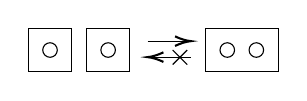
\begin{tikzpicture}[x=0.75pt,y=0.75pt,yscale=-0.7,xscale=0.7]
				%uncomment if require: \path (0,300); %set diagram left start at 0, and has height of 300
				%Shape: Square [id:dp8926747085287872] 
				\draw   (70,100) -- (100,100) -- (100,130) -- (70,130) -- cycle ;
				%Shape: Square [id:dp7911928154788817] 
				\draw   (110,100) -- (140,100) -- (140,130) -- (110,130) -- cycle ;
				%Shape: Circle [id:dp7972097445752802] 
				\draw   (80,115) .. controls (80,112.24) and (82.24,110) .. (85,110) .. controls (87.76,110) and (90,112.24) .. (90,115) .. controls (90,117.76) and (87.76,120) .. (85,120) .. controls (82.24,120) and (80,117.76) .. (80,115) -- cycle ;
				%Shape: Circle [id:dp2798464482392615] 
				\draw   (120,115) .. controls (120,112.24) and (122.24,110) .. (125,110) .. controls (127.76,110) and (130,112.24) .. (130,115) .. controls (130,117.76) and (127.76,120) .. (125,120) .. controls (122.24,120) and (120,117.76) .. (120,115) -- cycle ;
				%Straight Lines [id:da13754401873028943] 
				\draw    (152.11,108.89) -- (180,108.89) ;
				\draw [shift={(182,108.89)}, rotate = 180] [color={rgb, 255:red, 0; green, 0; blue, 0 }  ][line width=0.75]    (10.93,-3.29) .. controls (6.95,-1.4) and (3.31,-0.3) .. (0,0) .. controls (3.31,0.3) and (6.95,1.4) .. (10.93,3.29)   ;
				%Straight Lines [id:da986017380068096] 
				\draw    (154.11,119.89) -- (182,119.89) ;
				\draw [shift={(152.11,119.89)}, rotate = 0] [color={rgb, 255:red, 0; green, 0; blue, 0 }  ][line width=0.75]    (10.93,-3.29) .. controls (6.95,-1.4) and (3.31,-0.3) .. (0,0) .. controls (3.31,0.3) and (6.95,1.4) .. (10.93,3.29)   ;
				%Straight Lines [id:da5414382618735807] 
				\draw    (169.44,115) -- (179.44,125) ;
				%Straight Lines [id:da5354101657295061] 
				\draw    (169.44,125) -- (179.44,115) ;
				%Shape: Rectangle [id:dp9448845358260181] 
				\draw   (192,100) -- (242,100) -- (242,130) -- (192,130) -- cycle ;
				%Shape: Circle [id:dp5531546897679429] 
				\draw   (202,115) .. controls (202,112.24) and (204.24,110) .. (207,110) .. controls (209.76,110) and (212,112.24) .. (212,115) .. controls (212,117.76) and (209.76,120) .. (207,120) .. controls (204.24,120) and (202,117.76) .. (202,115) -- cycle ;
				%Shape: Circle [id:dp9053407831799309] 
				\draw   (222,115) .. controls (222,112.24) and (224.24,110) .. (227,110) .. controls (229.76,110) and (232,112.24) .. (232,115) .. controls (232,117.76) and (229.76,120) .. (227,120) .. controls (224.24,120) and (222,117.76) .. (222,115) -- cycle ;
			\end{tikzpicture}
		\end{minipage}
	\end{center}
	是满射, 但没有截面. 采用例 \ref{cohesion-family-of-sets} 对集合族的直观, 这就是说两个粘在一起的点无法分开 (右图).
	
	第二个例子是 $\mathsf {Fun}(B\mathbb{N},\mathsf {Set})$, 其中 $B\mathbb N$ 是将半群 $\mathbb N$ 视为单对象范畴. 这个范畴的对象是集合 $X$ 配备一个映射 $f\colon X\to X$. 态射
	\begin{center}
		\begin{minipage}
			{0.5\textwidth}
			% https://q.uiver.app/#q=WzAsNCxbMCwwLCJcXHswLDFcXH0iXSxbMSwwLCJcXHsqXFx9Il0sWzEsMSwiXFx7KlxcfSJdLFswLDEsIlxcezAsMVxcfSJdLFswLDFdLFsxLDJdLFswLDMsIjBcXG1hcHN0byAxXFxhdG9wIDFcXG1hcHN0byAwIiwyXSxbMywyXV0=
			\[\begin{tikzcd}[ampersand replacement=\&]
				{\{0,1\}} \& {\{*\}} \\
				{\{0,1\}} \& {\{*\}}
				\arrow[from=1-1, to=1-2]
				\arrow[from=1-2, to=2-2]
				\arrow["{0\mapsto 1\atop 1\mapsto 0}"', from=1-1, to=2-1]
				\arrow[from=2-1, to=2-2]
			\end{tikzcd}
			\]
		\end{minipage}
		\begin{minipage}
			{0.3\textwidth}
			\tikzset{every picture/.style={line width=0.75pt}} %set default line width to 0.75pt        
			\hspace{-2em}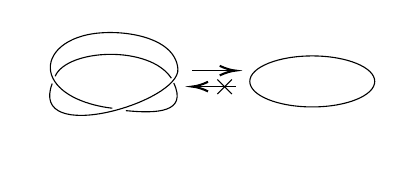
\begin{tikzpicture}[x=0.75pt,y=0.75pt,yscale=-0.7,xscale=0.7]
				%uncomment if require: \path (0,300); %set diagram left start at 0, and has height of 300
				%Curve Lines [id:da5256174669964437] 
				\draw    (57.33,121.78) .. controls (65.67,102.78) and (122.33,100.11) .. (137.33,123.11) ;
				%Curve Lines [id:da047957165101484955] 
				\draw    (55.33,126.78) .. controls (38.83,170.22) and (143.67,139.56) .. (141.83,116.67) .. controls (140,93.78) and (101,88.72) .. (80,93.11) .. controls (59,97.5) and (49.83,111.17) .. (55.83,123.17) .. controls (61.83,135.17) and (79.67,141.78) .. (96.67,143.78) ;
				%Curve Lines [id:da12392233177287926] 
				\draw    (106,145.44) .. controls (127.67,147.56) and (148.5,146.72) .. (139,126.44) ;
				%Shape: Ellipse [id:dp3575392941798332] 
				\draw   (191.33,125.33) .. controls (191.33,115.64) and (210.59,107.78) .. (234.33,107.78) .. controls (258.08,107.78) and (277.33,115.64) .. (277.33,125.33) .. controls (277.33,135.03) and (258.08,142.89) .. (234.33,142.89) .. controls (210.59,142.89) and (191.33,135.03) .. (191.33,125.33) -- cycle ;
				%Straight Lines [id:da8062516844631029] 
				\draw    (151.67,117.89) -- (179.56,117.89) ;
				\draw [shift={(181.56,117.89)}, rotate = 180] [color={rgb, 255:red, 0; green, 0; blue, 0 }  ][line width=0.75]    (10.93,-3.29) .. controls (6.95,-1.4) and (3.31,-0.3) .. (0,0) .. controls (3.31,0.3) and (6.95,1.4) .. (10.93,3.29)   ;
				%Straight Lines [id:da3938685457393487] 
				\draw    (153.67,128.89) -- (181.56,128.89) ;
				\draw [shift={(151.67,128.89)}, rotate = 0] [color={rgb, 255:red, 0; green, 0; blue, 0 }  ][line width=0.75]    (10.93,-3.29) .. controls (6.95,-1.4) and (3.31,-0.3) .. (0,0) .. controls (3.31,0.3) and (6.95,1.4) .. (10.93,3.29)   ;
				%Straight Lines [id:da45301762856536665] 
				\draw    (169,124) -- (179,134) ;
				%Straight Lines [id:da41762886315511905] 
				\draw    (169,134) -- (179,124) ;
			\end{tikzpicture}
		\end{minipage}
	\end{center}
	是满射, 但没有截面. 一个类似的例子是 $\operatorname{Sh}(S^1)$ 中 $S^1$ 的非平凡二重覆叠没有截面 (右图).
\end{example}

%
%\begin{proof}
%	假设\topos{} $\mathsf C$ 满足选择公理. 对任意满射 $p\colon X\to I$, 取截面 $s\colon I\to X$, 那么 $p^Y\colon X^Y\to I^Y$ 有截面 $s^Y\colon I^Y\to X^Y$, 从而 $X^Y\to I^Y$ 为满射, 即 $(-)^Y$ 保持满射.
%\end{proof}

\begin{prop}
	[label={IAC-technical-lemma}]
	{}
	假设\topos{} $\mathsf C$ 满足内蕴选择公理, 那么对其中任意满射 $f\colon Z\to X$, 都有 $\Pi_X(f) \to 1$ 是满射. 进一步, 记 $S=\Pi_X(f)$,
	则 $S^*Z\to S^*X$ (作为\topos{} $\mathsf C/S$ 中的映射, 定义见例 \ref{over-category-Sigma-adjunction}) 有截面.
\end{prop}

\begin{proof}
	回忆 $\Pi_X(f)$ 是 $f^X\colon Z^X\to X^X$ 沿 $\operatorname{id}_X\colon 1\to X^X$ 的拉回 (命题 \ref{pi-functor-absolute} 的证明), 而拉回保持满射 (命题 \ref{pullback-preserve-epis}), 故 $\Pi_X(f) \to 1$ 是满射. 映射 $S^*Z\to S^*X$ 的截面由取值映射 $S\times X\hookrightarrow Z^X\times X\overset{\operatorname{ev}}{\to} Z$ 给出.
\end{proof}

$\Pi_X(f)$ 是 ``$f$ 的截面的集合'', 所以内蕴选择公理是说满射在某种内蕴的意义上有截面.

\begin{prop}
	{(Diaconescu 定理)}
	满足内蕴选择公理的\topos{}一定是 Boole 的.
\end{prop}

\begin{proof}
	考虑任意子对象 $U\hookrightarrow X$. 由于单射是余核偶的等化子 (命题 \ref{topos-mono-regular}), 有 $U = \operatorname{eq}(X \rightrightarrows X \sqcup_U X)$. 我们的思路是考虑满射 $(X\sqcup X) \to (X\sqcup_U X)$ 的 ``截面'', 从而得到 $U\lor\neg U$.
	假设它有截面 $s\colon (X\sqcup_U X) \to (X\sqcup X)$, 如左图,
	\[\begin{tikzcd}[ampersand replacement=\&,column sep=small]
		V \& X \&\& {X\sqcup X} \& {1+1} \\
		\&\& {X\sqcup_U X}
		\arrow["t", from=1-4, to=1-5]
		\arrow["s"', hook, from=2-3, to=1-4]
		\arrow["{i_1}"{pos=0.7}, hook, from=1-2, to=2-3]
		\arrow["{si_1}"{pos=0.7}, shift left=2, hook', from=1-2, to=1-4]
		\arrow["{si_2}"'{pos=0.7}, hook', from=1-2, to=1-4]
		\arrow["{i_2}"'{pos=0.7}, shift right=2, hook, from=1-2, to=2-3]
		\arrow["f", from=1-1, to=1-2]
	\end{tikzcd}\quad
	\begin{tikzcd}[ampersand replacement=\&,column sep=small]
		V \& {X\sqcup X} \& {1+1} \\
		\& X
		\arrow["t",from=1-2, to=1-3]
		\arrow["{si_1f}", shift left=2, from=1-1, to=1-2]
		\arrow["f"', shift right=2, from=1-1, to=2-2]
		\arrow[from=1-2, to=2-2]
		\arrow["{si_2f}"', from=1-1, to=1-2]
	\end{tikzcd}\]
	那么 $s$ 为单射, 故对任何映射 $f\colon V\to X$, $f$ 等化 $i_1,i_2$ 当且仅当 $f$ 等化 $si_1,si_2$.
	而 $X\sqcup X \simeq X\times (1+1)$, 如右图,
	故 $f$ 等化 $si_1,si_2$ 等价于 $f$ 等化 $tsi_1,tsi_2$.
	这说明 $(U\hookrightarrow X)=\operatorname{eq}(tsi_1,tsi_2\colon X\rightrightarrows 1+1)$.
	
	由命题 \ref{IAC-technical-lemma}, 存在满射 $S\twoheadrightarrow 1$ 使得 $S^*(X\sqcup X)\to S^*(X\sqcup_U X)$ 有截面.
	
	\todo{}
	由于拉回是子对象 Heyting 代数的同态 (命题 \ref{subobject-lattice-Heyting-algebra}),
	
\end{proof}

另外, Bauer 的文章 (讲座) \cite{FSCM} 给出了 (外蕴) 选择公理推出排中律的一种证明.

% 第二章 位象理论
\chapter{位象: 无点拓扑学}

%\todo{变成单独的一章?}

常常拓扑空间的重点不在于\emph{点}, 而在于开集, 以及开集之间的关系.
将开集的性质提炼出来, 使其不再依赖于点, 就成为\emph{位象} (locales) 的概念. 它是介于拓扑空间和景之间的一个推广.\footnote{说位象是拓扑空间的 ``推广'' 不甚准确, 因为一般拓扑空间到位象的对应不是全忠实的 (有的空间开集太少). 但是 ``好'' 的空间范畴如 Hausdorff 空间范畴确实嵌入位象的范畴.}
位象理论又称为\emph{无点拓扑学} (pointless topology\footnote{双关笑话: 无点拓扑学不是 pointless (无用的).})

Andr\'e Joyal \cite{Joyal-Crash-Course} 建议在\topos{}理论之前先学习位象理论.

在高阶的观点中, 位象又可称作 $0$-\topos{}.

\newcommand{\fm}{位格}

\section{基本概念}

\begin{definition}
	{(\fm{})}
	\emph{\fm{}} (frame, 又称 local lattice)\footnotemark 是满足如下条件的偏序集:
	\begin{itemize}
		\item 存在有限交 $\wedge$ 与任意并 $\bigvee$, 其中一族元素的\emph{交} (meet) 是指同时小于等于这些元素的最大元, \emph{并} (join) 是指同时大于等于这些元素的最小元;
		\item 有结合律
		$$
		a \wedge \bigvee_{i \in I} b_i = \bigvee_{i \in I} (a \wedge b_i),
		$$
		其中 $I$ 是任意集合.
	\end{itemize}
	
	\fm{}的态射是偏序集之间保持有限交与任意并的态射. \fm{}的范畴记为 $\mathsf {Frm}$.
\end{definition}
\footnotetext{Frame 一词似乎没有通行的中文翻译. 这里试译为\fm{}, 因为它是一种与拓扑相关的格 (lattice).}
\begin{remark}
	{}
	由于任意交可由任意并表示,
	$$
	\bigwedge A = \bigvee \big\{ b \colon b\leq a \ \forall a\in A\big\},
	$$
	可以证明\fm{}中任意交也存在, 即\fm{}是\emph{完备格} (complete lattice). 但由定义, \fm{}的态射不一定保持任意交.
\end{remark}

\begin{definition}
	[label={locale-definition}]
	{(位象)}
	\emph{位象} (locale) 是\fm{}的形式对偶,
	即我们定义位象的范畴 $\mathsf {Loc}$ 是位格范畴 $\mathsf {Frm}$ 的对偶范畴.
	
	对于位象 $X$, 我们记对应的\fm{}为 $\mathcal O(X)$, 称其中的元素为 $X$ 的\emph{开子集}或\emph{开子空间}; 对于位象的态射 $f \colon X \to Y$,
	记对应的\fm{}的态射为 $f^* \colon \mathcal O(Y) \to \mathcal O(X)$.
\end{definition}

\begin{remark}
	{}
	\fm{}与位象的对偶类似于环与仿射概形的对偶,
	是代数--几何对偶的一例.
	%位象的定义中引入的记号都是为了体现这种对偶.
\end{remark}

\begin{example}
	{(拓扑空间作为位象)}
	拓扑空间 $X$ 的开集范畴 $\operatorname{Open}(X)$ 构成一个\fm{}.
	对于连续映射 $f \colon X \to Y$,
	我们有反向的\fm{}态射 $f^* \colon \operatorname{Open}(Y) \to \operatorname{Open}(X)$,
	将 $Y$ 的开集 $U$ 映射到 $X$ 的开集 $f^{-1}(U)$, 保持有限交与任意并.
	这构成了函子 $\operatorname{Open} \colon \mathsf {Top} \to \mathsf {Frm}^{\op}$; 由定义 $\mathsf {Loc} = \mathsf {Frm}^{\op}$, 我们得到函子 $$\operatorname{Open} \colon \mathsf {Top} \to \mathsf {Loc}.$$
\end{example}

\begin{example}
	{(环的谱作为位象)}
	在代数几何中, (交换) 环的谱 $\operatorname{Spec}A$ 是由 $A$ 的素理想的集合赋予 Zariski 拓扑定义的. 然而, 我们也可以直接刻画谱的 ``基础开集'' $U_f$ 生成的\fm, 从而不需要使用环的素理想\footnotemark:
	$$
	\mathcal O(\operatorname{Spec}A):= \big\langle U_f\colon f\in A\mid U_0 = \bot, U_1 = \top,
	U_{f+g} \leq U_f \vee U_g, U_{fg} = U_f \wedge U_g \big\rangle.
	$$
	(\fm{}就像群, 环等代数结构一样, 可使用生成元和关系刻画, 并且可由给定生成元的 ``自由代数'' 的商得到.)
	
	将 $U_f$ 想象为一个空间上函数 $f$ ``非零'' 的地方,
	$f+g$ 非零的地方包含于 $f$ 与 $g$ 各自非零的地方的并,
	而 $fg$ 非零的地方恰为两者的交.
	可以证明如此定义的位象 $\operatorname{Spec}A$ 正是传统上定义的拓扑空间 $\operatorname{Spec}A$.
\end{example}
\footnotetext{Jacob Lurie 在 \emph{Derived Algebraic Geometry V: Structured Spaces} 第 37 页写道, ``It is in some sense coincidental that $\operatorname{Spec} A$ is described by a topological space. What arises more canonically is the lattice of open subsets of $\operatorname{Spec} A$, which is generated by basic open sets of the form $U_f$. This lattice naturally forms a \emph{locale} ...'' \par
	值得一提的是, 构造主义数学青睐这种位象的观点, 因为环的素理想的存在性依赖选择公理. 关于构造主义数学与位象, 我们推荐读者观看 Andrej Bauer 的讲座. \url{https://www.youtube.com/watch?v=21qPOReu4FI}}

%\begin{example}
%	[label={complete-boolean-algebras}]
%	{(完备 Boole 代数)}
%	Boole 代数是满足如下条件的
%\end{example}

\begin{example}
	{(点作为位象)}
	单点空间 $\text{pt}$ 对应的位象记作 $1 = \operatorname{Open}(\text{pt})$.
	它对应的位格是两个元素的偏序集 $\mathcal O(1) = \{\bot,\top\}$.
	位象 $1$ 也称为\emph{终位象} (terminal locale).
\end{example}

% 下面的定义表明从位象中可以还原出 ``点'' 的概念.

\begin{definition}
	[label={points-of-locale}]
	{(位象的点)}
	定义位象 $X$ 的\emph{点}为位象的态射 $p\colon 1 \to X$.
	记位象 $X$ 的点的集合为 $\operatorname{Pt}(X)$.
\end{definition}

在\fm{}的层面, 位象 $X$ 的一个点 $p\colon 1 \to X$ 是保持有限交与任意并的态射 $p^*\colon \mathcal O(X) \to \{\bot,\top\}$.
考虑 $\top$ 的原像, 我们得到 $\mathcal O(X)$ 的一个\emph{完全素滤子} (completely prime filter). (偏序集中的\emph{滤子}是关于交封闭的向上封闭子集, 称 $F$ 为完全素滤子是指当 $\bigvee_i U_i \in F$ 时, 至少有一个 $U_i$ 属于 $F$.)

\begin{remark}
	{}
	滤子是理想的 ``对偶''. 我们有如下类比: 态射 $\mathcal O(X)\to \{\bot,\top\}$ 中 $\top$ 的原像是完全素滤子, 类似于环同态 $A\to k$ 的核是素理想 ($k$ 为整环). 位象 $X$ 的点对应 $\mathcal O(X)$ 的完全素滤子, 类似于谱 $\operatorname{Spec}A$ 的点对应环 $A$ 的素理想.
\end{remark}

对每个元素 $U\in\mathcal O(X)$, 规定 $\operatorname{Pt}(X)$ 的子集
$\{p \in \operatorname{Pt}(X) \colon p^*(U) = \top\}$ 为开集,
我们得到了 $\operatorname{Pt}(X)$ 上的一个拓扑. 于是有函子
$$\operatorname{Pt} \colon \mathsf {Loc} \to \mathsf {Top}.$$

\begin{prop}
	[label={top-loc-adjunction}]
	{}
	拓扑空间与位象之间有伴随
	% https://q.uiver.app/#q=WzAsMixbMCwwLCJcXG1hdGhzZiB7VG9wfSJdLFsxLDAsIlxcbWF0aHNmIHtMb2N9Il0sWzAsMSwiXFxvcGVyYXRvcm5hbWV7T3Blbn0iLDAseyJvZmZzZXQiOi0yfV0sWzEsMCwiXFxvcGVyYXRvcm5hbWV7UHR9IiwwLHsib2Zmc2V0IjotMn1dLFsyLDMsIiIsMCx7ImxldmVsIjoxLCJzdHlsZSI6eyJuYW1lIjoiYWRqdW5jdGlvbiJ9fV1d
	\[\begin{tikzcd}[ampersand replacement=\&]
		{\mathsf {Top}} \& {\mathsf {Loc}.}
		\arrow[""{name=0, anchor=center, inner sep=0}, "{\operatorname{Open}}", shift left=2, from=1-1, to=1-2]
		\arrow[""{name=1, anchor=center, inner sep=0}, "{\operatorname{Pt}}", shift left=2, from=1-2, to=1-1]
		\arrow["\dashv"{anchor=center, rotate=-90}, draw=none, from=0, to=1]
	\end{tikzcd}\]
\end{prop}

上述伴随远远不是范畴等价; 首先, 从拓扑空间对应的位象中不一定能重构出原来的拓扑空间, 例如所有平凡拓扑对应的位象都是终位象 $1$.

然而, 对于分离性较好的空间, 其对应的位象确实能重构出这个空间:
\begin{definition}
	{(清晰空间)}
	设 $X$ 为拓扑空间. 若命题 \ref{top-loc-adjunction} 中伴随的单位 $X \to \operatorname{Pt}\operatorname{Open}(X)$ 是同胚,
	则称 $X$ 为\emph{清晰空间} (sober space\footnotemark). 换言之, 清晰空间的范畴是上述伴随给出的等价的满子范畴 (命题 \ref{adjoint-full-subcategory-equivalence}).
\end{definition}
\footnotetext{Sober 的原义是清醒, 未喝醉. 直观上一个 sober 空间中的点没有过于 ``糊在一起'', 清晰可辨.}

\begin{prop}
	{}
	Hausdorff ($T_2$) 空间都是清晰空间, 清晰空间都是 $T_0$ 空间; 而清晰与 $T_1$ 互不蕴涵, 例如 Sierpi\'nski 空间清晰而不 $T_1$, 无限集上的余有限拓扑 $T_1$ 而不清晰.
\end{prop}

另一方面, 从一个位象的所有点的信息也无法重构出这个位象: 下面的例子表明一个位象甚至可能没有点!

\begin{example}
	{(没有点的位象的例子: 完备无原子 Boole 代数)}
	
	\emph{Boole 代数}是有二元交, 二元并以及补运算 (满足适当条件) 的偏序集; \emph{完备 Boole 代数}是指存在任意交和任意并的 Boole 代数.
	由定义, 完备 Boole 代数是\fm.
	称偏序集中的一个元素为\emph{原子}, 是指除 $\bot$ 以外没有比它更小的元素.
	对任何完备 Boole 代数 $B$, 设 $P$ 是 $B$ 的完全素滤子,
	则 $\bigwedge P$ 是 $B$ 的原子. 这是因为, 假设 $x < \bigwedge P$,
	则 $x\notin P$, 从而由 $\top=x\vee\neg x\in P$, 得 $\neg x \in P$. 这说明 $x<\neg x$, 故 $x=\bot$.
	因此, 完备无原子 Boole 代数对应没有点的位象.
	下面是两个完备无原子 Boole 代数的例子.
	
	\begin{itemize}
		\item 设 $(X,\mathcal A,\mu)$ 为 $\sigma$-有限测度空间, $N\subset \mathcal A$ 为零测集的理想,
		那么商代数 $\mathcal A / N$ 是完备 Boole 代数; 并且当 $\mu$ 无原子 (没有正测度的点) 时, $\mathcal A/N$ 无原子.
		\item	
	设 $X$ 为拓扑空间. 对于开集 $U\subset X$, 定义 $\neg U$ 是 $U$ 的补集的内部.
	考虑偏序集
	$$
	\text{RO}(X)
	=
	\big\{U\in\operatorname{Open}(X)\mid U = \neg\neg U\big\},
	%P\mathbb{N}\big/ \sim,\quadA\sim B \Leftrightarrow A\setminus B, B\setminus A\text{为有限集}.
	%$$% 是 $\mathbb{N}$ 的子集在相差有限个元素的等价关系下构成的偏序集.
	$$
	称为 $X$ 的\emph{正则开集代数} (regular open algebra). 可以证明 $\text{RO}(X)$ 也是一个完备 Boole 代数\footnotemark. 例如其中的任意并由下式给出:
	$$
	\bigvee_{i\in I}U_i = \neg\neg\Big(\bigcup_{i\in I}U_i\Big).
	$$
	
	若取空间 $X$ 为欧氏空间, 则 $\text{RO}(X)$ 没有原子 (任何正则开集内都有一个更小的正则开集).
	\end{itemize}
\end{example}
\footnotetext{\url{https://planetmath.org/regularopenalgebra}}

\subsection{子位象}

正如许多 ``空间'' 的概念 (拓扑空间, 向量空间, 概形 ...) 一样, 位象有一种自然的 ``子空间'' 的概念; 当然, 子位象不是通过点集, 而是通过开集的代数定义的.

\begin{definition}
	{(子位象)}
	设 $X$ 为位象. 定义 $X$ 的\emph{子位象} (sublocale) $Y$ 如下: $\mathcal O(Y)$ 为 $\mathcal O(X)$ 在一个保持交与任意并运算的等价关系 (即 $\mathcal O(X)\times\mathcal O(X)$ 的子\fm{}) $\equiv_Y$ 下的\emph{商}. 直观上, 这个等价关系是说两者与子空间的 ``交'' 相同.
	
	对于两个子位象 $Y,Z$, 若 $U\equiv_Z V \Rightarrow U\equiv_Y V$, 则称 $Y$ \emph{包含于} $Z$.
\end{definition}

子位象是\fm{}范畴 $\mathsf {Frm}$ 中的\emph{正则满射}, 即位象范畴 $\mathsf {Loc}$ 中的\emph{正则单射} (定义 \ref{regular-epi-and-mono}).

对于位象 $X$, $\mathcal O(X)$ 的元素可视为其开子空间.

\begin{definition}
	{(开子位象)}
	设 $X$ 为位象, $W\in\mathcal O(X)$. 定义 $X$ 的\emph{开子位象} $W$:
	$$U \equiv_W V \quad \text{当且仅当} \quad U\cap W = V \cap W.$$
\end{definition}



\subsection{测度与随机性}

本小节介绍 Alex Simpson 的文章 \cite{SIMPSON20121642} 引入的\emph{随机序列的位象}. 它是 $0$ 和 $1$ 组成的所有可数序列的空间的 ``子空间'', 但没有任何一个序列属于这个子空间, 因为 ``一个确定的序列永远不是随机序列''.

首先引入位象上的测度; 这是测度空间的一个推广. 设 $X$ 为位象, 其上的\emph{测度}是满足如下条件的函数 $\mu\colon \mathcal O(X)\to [0,+\infty]$:

\begin{definition}
	{(位象上的测度)}
	\begin{itemize}
		\item $\mu(\bot) = 0$,
		\item $x\leq y \Rightarrow \mu(x)\leq \mu(y)$,
		\item $\mu(x)+\mu(y)=\mu(x\vee y)+\mu(x\wedge y)$,
		\item 对任意 (可数) 递增序列 $x_1\leq x_2\leq\cdots$, $\mu(\bigvee_i x_i)=\sup_{i}\mu(x_i)$.
	\end{itemize}
	若 $\mu(\top)=1$, 称 $\mu$ 为\emph{概率测度}.
\end{definition}

\begin{propdef}
	{(随机元素的子位象)}
	设位象 $X$ 上有测度 $\mu$. 定义 $X$ 的 \emph{$\mu$-随机元素的子位象} $\operatorname{Ran}_\mu(X)$ 如下:
	$$
	U\equiv_{\operatorname{Ran}_\mu(X)} V \quad \text{当且仅当}\quad \mu(U\cap V) = \mu(U\cup V).
	$$
	可以验证 $\equiv_{\operatorname{Ran}_\mu(X)}$ 确实是一个等价关系; 直观上, 这个等价关系是相差一个 $\mu$-零测集.
\end{propdef}

\begin{prop}
	{}
	设 $X$ 为清晰空间, 带有测度 $\mu$, 则 $\operatorname{Ran}_\mu(X)$ 的点一一对应于 $X$ 的原子.
\end{prop}

\todo{解释原子的含义}

\todo{}

\section{位象与逻辑}

\philoquote{[A locale is a] propositional geometric theory pretending to be a space.}{Steven Vickers}

建议在阅读本节之前阅读附录 \ref{first-order-languages} 节, 尤其关注几何逻辑的内容.

% frame = complete Heyting algebra (但作为范畴不同构)

我们将建立如下对应.

\begin{itemize}
	\item 位象 = 命题逻辑理论
	\item 开集 = 命题
	\item 点 = 模型
\end{itemize}

\subsection{经典命题逻辑与 Lindenbaum 代数}

Lindenbaum 代数是用代数方法研究逻辑的工具, 代数--几何对偶. 粗略地说, 它是一个理论中的 ``命题的代数''; 在经典逻辑的情形, 它就是 \emph{Boole 代数}, 而对应的 ``空间'' 是 \emph{Stone 空间}, 两者的对偶由 \emph{Stone 表示定理}描述.

设 $\Sigma$ 是由若干命题符号 $p,q,r,\cdots$ 组成的符号表\footnote{在定义 \ref{def-first-order-signature} 的框架中, 我们可以说 $\Sigma$ 包括 $0$ 个类型, $0$ 个函数符号 (固然, 因为 $\Sigma$ 中没有类型), 以及若干个 $0$ 元关系符号 $p,q,r,\cdots$.}.
定义 $\mathsf {Sen}_\Sigma$ 为 $\Sigma$ 上由 $\lor,\land,\neg,\Rightarrow,\top,\bot$ 组成的公式\footnote{这里的公式也可以放在定义 \ref{formula} 的框架中. 注意, 在这个框架中没有等式 $p=q$, 因为 $p,q$ 不是某个类型的项 ($\Sigma$ 中没有类型), 而是 $0$ 元关系符号.}的集合, 包括 $(p\land q)\Rightarrow r$, $p\lor\neg p$, $p\Rightarrow\bot$ 等等.

\begin{definition}
	{}
	在经典逻辑中, 对于符号表 $\Sigma$ 上的命题理论 $\mathbb T$ (即一些公理的集合), 定义 $\mathbb T$ 的 \emph{Lindenbaum 代数} $\text{LA}_{\mathbb T}$ 为 $\Sigma$ 上公式的 $\mathbb T$-\emph{可证等价类}构成的 Boole 代数:
	$$
	\text{LA}_{\mathbb T} := \mathsf {Sen}_\Sigma \big/ {\equiv_{\mathbb T}},\quad
	\text{其中 $\phi\equiv_{\mathbb T} \psi$ 当且仅当 $\mathbb T$ 可证 $\phi\Leftrightarrow\psi$}.
	$$
\end{definition}

\begin{definition}
	{(命题理论之间的态射)}
	对于两个命题理论 $(\Sigma,\mathbb T)$, $(\Sigma',\mathbb T')$, 定义态射 $f\colon \mathbb T \to \mathbb T'$ 为映射 $f\colon \Sigma \to \mathsf {Sen}_{\Sigma'}$, 它自然诱导映射 $\mathsf {Sen}_\Sigma\to \mathsf {Sen}_{\Sigma'}$, 使得 $f$ 保持公理, 即 $f(\mathbb T)\subset \mathbb T'$. 等价地, $f$ 为 Boole 代数同态 $\text{LA}_{\mathbb T} \to \text{LA}_{\mathbb T'}$.
\end{definition}

\begin{remark}
	{}
	命题理论的态射可类比于环同态: 对于两个环 $R=\mathbb{Z}[x_1,\cdots,x_n]/I$ 与 $R'=\mathbb{Z}[y_1,\cdots,y_m]/J$, 环同态 $f\colon R\to R'$ 为映射 $\{x_1,\cdots,x_n\}\to R'$ (它自然诱导映射 $\mathbb{Z}[x_1,\cdots,x_n]\to \mathbb{Z}[y_1,\cdots,y_m]$), 使得 $f(I)\subset J$.
\end{remark}

\begin{definition}
	{(命题理论的模型)}
	一个命题理论 $(\Sigma,\mathbb T)$ 的\emph{经典模型} (classical model, 又称\emph{解释}, interpretation) 是一个函数 $f\colon \Sigma \to \{\top,\bot\}$, 它自然诱导一个映射 $\bar f\colon \mathsf {Sen}_\Sigma\to\{\top,\bot\}$, 使得 $\bar f(\mathbb T)\subset \{\top\}$. 记 $\mathbb T$ 的经典模型的集合为 $\text{Mod}(T)$.
	
	一般地, 对任意 Boole 代数 $A$, $(\Sigma,\mathbb T)$ 的 \emph{$A$-模型}是一个映射 $f\colon \Sigma \to A$, 它自然诱导一个映射 $\bar f\colon \mathsf {Sen}_\Sigma\to A$, 使得 $\bar f(\mathbb T)\subset \{\top\}$. 记 $\mathbb T$ 的 $A$-模型的集合为 $\text{Mod}_A(\mathbb T)$.
\end{definition}



\begin{prop}
	{}
	命题理论 $(\Sigma,\mathbb T)$ 的 $A$-模型一一对应于 Boole 代数同态 $\text{LA}_{\mathbb T} \to A$.
\end{prop}

\begin{proof}
	设 $f\colon \Sigma\to A$ 为 $\mathbb T$ 的 $A$-模型. 我们需要证明 $\bar f\colon \mathsf {Sen}_\Sigma\to A$ 将 $\mathbb T$-等价的公式对应到相同的元素. 若 $\phi \equiv_{\mathbb T} \psi$, 设 $\mathbb T$ 对 $\phi \Leftrightarrow\psi$ 的证明用到了公理 $t_1,\cdots,t_n$, 那么由经典逻辑的性质可知
	$$
	\big( \bar f(t_1) \land \cdots \land \bar f (t_n) \big) \leq \big( \bar f(\phi) \Leftrightarrow \bar f(\psi) \big),
	$$
	但由 $f$ 是 $\mathbb T$ 的 $A$-模型, $\bar f(t_1)=\cdots = \bar f(t_n) = \top\in A$, 这说明 $\bar f(\phi) = \bar f(\psi)$.
\end{proof}

\begin{remark}
	{}
	上述命题可类比于环同态的如下性质:
	对于多项式 $f_1,\cdots,f_m\in \mathbb{Z}[x_1,\cdots,x_n]$ 以及任何环 $A$, 集合
	$$
	\big\{
	(a_1,\cdots,a_n)\in A^n\mid f_i(a_1,\cdots,a_n)=0\,(i=1,2,\cdots,m)
	\big\}
	$$
	一一对应于环同态 $\mathbb{Z}[x_1,\cdots,x_n]/(f_1,\cdots,f_m) \to A$.
\end{remark}

\begin{remark}
	{}
	由上述命题, $\mathbb T$ 的经典模型一一对应于 Boole 代数同态 $\text{LA}_{\mathbb T} \to \{\top,\bot\}$, 即 $\text{LA}_{\mathbb T}$ 的\emph{超滤}.
	回忆位象 $X$ 的点是\fm{}同态 $\mathcal O(X) \to \{\top,\bot\}$, 即 $\mathcal O(X)$ 的完全素滤子. 两种情形的区别在于逻辑规则: Boole 代数中没有任意并, 而有排中律; \fm{}中有任意并, 没有排中律.
\end{remark}

\begin{prop}
	{}
	命题理论的态射 $f\colon (\Sigma,\mathbb T) \to (\Sigma',\mathbb T')$ 诱导模型的映射 $\text{Mod}_A(\mathbb T') \to \text{Mod}_A(\mathbb T)$.
\end{prop}

注意方向的反转 (这是代数--几何对偶的一部分).
%集合 $\text{Mod}(\mathbb T)$ 可附加一个拓扑, 以 $\{f\in\text{Mod}(\mathbb T)\mid \bar f(\phi)=\top\}$ 为开集基 ($\phi$ 取所有公式).

\begin{definition}
	{(Stone 空间)}
	称紧的完全不连通 (仅有的连通分支为单点集) Hausdorff 空间为 \emph{Stone 空间}. 等价的定义是紧且\emph{完全分离} (任何两个点都能通过把空间分成两个连通分支而分开) 的空间.
\end{definition}

\begin{propdef}
	{}
	对 Boole 代数 $B$, 在集合 $\operatorname{Hom}_{\mathsf {BooleAlg}}(B,\{\top,\bot\})$ 上附加一个拓扑, 以 $\{b\in B\mid f(b)=\top\}$ 为开集基; 那么 $\operatorname{Hom}_{\mathsf {BooleAlg}}(B,\{\top,\bot\})$ 是 Stone 空间.
\end{propdef}

\begin{proof}
	首先证明 $\operatorname{Hom}_{\mathsf {BooleAlg}}(B,\{\top,\bot\})$ 是紧空间. 事实上, 它是积空间 $\{\top,\bot\}^{B}$ 的闭子集. 由 Tychonoff 定理, 紧空间的任意乘积是紧空间, 故 $\{\top,\bot\}^{B}$ 是紧空间, 从而 $\operatorname{Hom}_{\mathsf {BooleAlg}}(B,\{\top,\bot\})$ 是紧空间.
	\todo{}
\end{proof}

\begin{prop}
	{(Stone 对偶)}
	
	Boole 代数与 Stone 空间之间存在范畴等价
	% https://q.uiver.app/#q=WzAsMixbMCwwLCJcXG1hdGhzZiB7Qm9vbGVBbGd9Il0sWzIsMCwiXFxtYXRoc2Yge1N0b25lU3B9Il0sWzAsMSwiXFxvcGVyYXRvcm5hbWV7SG9tfSgtLFxce1xcdG9wLFxcYm90XFx9KSIsMix7Im9mZnNldCI6Mn1dLFsxLDAsIlxcb3BlcmF0b3JuYW1le0hvbX0oLSxcXHtcXHRvcCxcXGJvdFxcfSkiLDIseyJvZmZzZXQiOjJ9XV0=
	\[\begin{tikzcd}[ampersand replacement=\&]
		{\mathsf {BooleAlg}} \&\& {\mathsf {StoneSp}.}
		\arrow["{\operatorname{Hom}_{\mathsf {BooleAlg}}(-,\{\top,\bot\})}"', shift right=2, from=1-1, to=1-3]
		\arrow["{\operatorname{Hom}_{\mathsf {StoneSp}}(-,\{\top,\bot\})}"', shift right=2, from=1-3, to=1-1]
	\end{tikzcd}\]
\end{prop}

\begin{proof}
	
\end{proof}

\todo{}

% sublocale 与 product locale 对应的理论是什么


% 第三章 Grothendieck \topos{}

\chapter{Grothendieck \topos{}与空间的概念}

\philoquote{
	Le point de vue et le langage des faisceaux introduit par Leray nous a amené à regarder les ``espaces'' et ``variétés'' en tous genres dans une lumière nouvelle.
	Ils ne touchaient pas, pourtant, à la notion même d'espace, se contentant de nous faire appréhender plus finement, avec des yeux nouveaux, ces traditionnels ``espaces'',
	déjà familiers à tous.
	
	~\\
	
	%Or, il s'est avéré que cette notion d'espace est inadéquate pour rendre compte des ``invariants topologiques'' les plus essentiels qui expriment la ``forme'' des variétés algébriques ``abstraites'' (comme celles auxquelles s'appliquent les conjectures de Weil), voire celle des ``schémas'' généraux (généralisant les anciennes variétés).
	\quad[C]e qui compte vraiment dans un espace topologique, ce ne sont nullement ses ``points'' ou ses sous-ensembles de points, et les relations de proximité etc entre ceux-ci, mais que ce sont les faisceaux sur cet espace, et la catégorie qu'ils forment.
	}{Grothendieck, Récoltes et Semailles\footnotemark}
\footnotetext{这两段评注出自 Grothendieck 的自传 ``收获与播种''.
	
Leray 引入的层的观点和语言使我们以新的视角看待各种 ``空间'' 和 ``流形''. 然而, 它们并未触及空间的概念本身, 只是用新的眼光更加精细地理解那些传统的, 人们早已熟知的空间. % 然而, 事实证明, 这种空间的概念无法准确表达 ``抽象'' 代数簇 (如 Weil 猜想所使用的代数簇) 以及 (推广了传统代数簇的) 一般的 ``概形'' 最本质的 ``拓扑不变量''.

拓扑空间中真正重要的不是它的 ``点'' 或点集的子集, 以及点之间的邻近关系等等, 而是这个空间上的层, 以及它们构成的范畴.
}

\label{chapter-grothendieck-toposes}

\topos{}的概念最早由 Grothendieck 提出. 他将其命名为 topos\footnote{希腊文, ``位置''}, 意在表达这个概念是能够承载拓扑与几何直观的最广泛的概念.

拓扑空间 $X$ 上的层构成一个\topos{} $\operatorname{Sh}(X)$, 称为\emph{层\topos{}} (sheaf topos). 这个\topos{}很大程度上反映了空间 $X$ 的信息. Grothendieck 将层的概念由拓扑空间推广到了最一般的语境, 由此得到一种极为广泛的空间概念; 他将其命名为\emph{景} (site). 景上的层构成的范畴即是所谓 \emph{Grothendieck \topos{}}.

Grothendieck 的想法是, 一个\topos{}不一定来自普通的拓扑空间, 但由于它与 (拓扑空间上的) 层范畴极为相似的性质, 我们可以设想它是一个假想的空间上的层范畴, 即其中的对象是这个假想的空间之上的层. 这个想法也可视为代数--几何对偶的一例: 正如 Gelfand 考虑 Hausdorff 空间上的复值连续函数, Grothendieck 考虑空间上的 ``集合值连续函数''.

% 层\topos{}中的真值是 $X$ 的一个开集, 代表命题 ``在 $X$ 上的何处成立''. 从外部看, $X$ 上的层可视为沿着 $X$ ``一族连续变化的对象'', 而在层\topos{}的语言中, 一个层仿佛单个的对象.

% 这几句话放这里不合适. 该放哪里?

我们从层的一般概念讲起.

\section{预层}

%\subsection{范畴上的预层}

\begin{definition}{(小范畴上的预层)}
    设 $\mathsf C$ 是小范畴. 定义 $\mathsf C$ 上的\emph{预层} (presheaf) 是 $\mathsf C^{\op}$ 到 $\mathsf {Set}$ 的函子.
    记 $\mathsf C$ 上的预层范畴为 $\widehat {\mathsf C} := \mathsf {Fun}(\mathsf C^{\op},\mathsf {Set})$.
\end{definition}

预层 $F \colon \mathsf C^{\op} \to \mathsf {Set}$ 可视为一个假想的空间, 可用 $\mathsf C$ 的对象来\emph{探测} (probe). 我们对这个 ``空间'' 仅有的了解, 是 $\mathsf C$ 的对象 $c$ 到 $F$ 的假想态射 ``$c\to F$'' 的集合 $F(c)$, 以及态射 $d\to c$ 与假想态射 ``$c\to F$'' 的复合 $d\to c\to F$, 这给出集合的映射 $F(c) \to F(d)$.

由 $\mathsf C$ 的对象 $c$, 可得 $\mathsf C$ 上的预层 $\operatorname{Hom}_{\mathsf C}(-,c)$. 这事实上是 $\mathsf C$ 到 $\widehat {\mathsf C}$ 的嵌入.
\begin{definition}
    {(米田嵌入)}
    小范畴 $\mathsf C$ 的\emph{米田嵌入}是指函子
    $\yo\colon \mathsf C \to \widehat{\mathsf C}$,
    $c\mapsto \yo(c) = \operatorname{Hom}_{\mathsf C}(-,c)$. 米田嵌入的像 $\yo(c)$ 称为\emph{可表函子} (representable functor).
\end{definition}

\begin{remark}{}
    米田嵌入也可定义为函子 $\operatorname{Hom}\colon \mathsf C^{\op}\times\mathsf C \to \mathsf {Set}$ 对应的函子
    $\mathsf C \to \mathsf {Fun}(\mathsf C^{\op},\mathsf {Set})$. 这是因为 $\widehat {\mathsf {C}}$ 是 ``范畴的范畴'' 中的指数对象.
\end{remark}

对于预层 $F \in \widehat {\mathsf C}$, 前面提到的 $c$ 到 $F$ 的 ``假想态射'' 可赋予真实的含义, 它就是 $\yo(c)$ 到 $F$ 的态射 (自然变换). 这样一个自然变换由 $\operatorname{id}_c \in \yo(c)(c)$ 的像 ($F(c)$ 的元素) 唯一决定, 因此有如下的结论.
\begin{prop}{(米田引理)}
    对任意 $X \in \widehat {\mathsf C}$, 有自然同构
    $$
    \operatorname{Hom}_{\widehat {\mathsf C}}(\yo(c),F) \simeq F(c).
    $$
\end{prop}

\begin{remark}{}
    米田引理在逻辑上是平凡的; 它带给我们的\emph{观点}, 即 $\mathsf C$ 的对象 $c$ 可\emph{等同于}函子 $\yo(c)$, 比命题本身更重要. 后面我们将大量使用这种观点.

    关于米田引理的更多应用, 以及预层范畴的更多性质, 见附录 \ref{yoneda} 节.
\end{remark}

\subsection{常见的预层范畴}

\begin{example}
    {(集合)}
    记 $\mathsf {1}$ 为仅有一个对象和一个态射的范畴.
    $\mathsf {1}$ 上的预层范畴 $\widehat {\mathsf 1} = \mathsf {Set}^{\mathsf {1}^\op}$ 等同于集合范畴 $\mathsf {Set}$.
    它也可视为单点空间上的层范畴;
    它在\topos{}中扮演的角色等同于一个点在拓扑空间中扮演的角色.
\end{example}

\begin{example}
    [label={Simplicial-Sets}]
    {(单纯集)}
    令范畴 $\Delta$ 为有限全序集 $[0],[1],[2],\cdots$ 与保序映射构成的范畴, 其中 $[n] = \{0,1,\cdots,n\}$, 称映射 $f \colon [n] \to [m]$ 为保序映射是指当 $i\leq j$ 时 $f(i)\leq f(j)$.
    我们将 $[n]$ 想象为 $n$ 维单纯形.
    称范畴 $\Delta$ 为\emph{单纯范畴} (simplicial category).

    $\Delta$ 上的预层称为\emph{单纯集} (simplicial set), 也就是可用单纯形来探测的空间. 记单纯集范畴为
    $\mathsf {sSet}=\widehat {\Delta}=\mathsf {Fun}(\Delta^{\op},\mathsf {Set})$.
    
    对于单纯集 $X \colon 
    \Delta^{\op} \to \mathsf {Set}$,
    $X([n])$ 表示 $X$ 中 $n$ 维单形的集合,
    其中含有退化的单形.
    记米田嵌入 $\yo([n])$ 为 $\Delta^n$,
    米田引理告诉我们
    $$
    X([n]) \simeq \operatorname{Hom}_{\mathsf {sSet}}(\Delta^n,X),
    $$
    因此如上关于 $X([n])$ 的解释是准确的.
\end{example}

\begin{example}
    {(有向图)}
    有向图可用类似于单纯集 (例 \ref{Simplicial-Sets}) 的方式定义.
    考虑范畴
    $$
    \mathsf C=
    \Big\{\!
    \begin{tikzcd}[ampersand replacement=\&]
	{[0]} \& {[1]}
	\arrow["s", shift left, from=1-1, to=1-2]
	\arrow["t"', shift right, from=1-1, to=1-2]
    \end{tikzcd}
    \!\Big\},
    $$
    其中 $s,t\colon [0]\to [1]$
    分别将 $0\in [0]$ 映射到 $0\in [1]$ 和 $1\in [1]$.
    那么 $\mathsf C$ 上的预层 $X\colon \mathsf C^{\op}\to\mathsf {Set}$ 可视为有向图:
    $X([0])$ 是有向图的顶点集, $X([1])$ 是有向图的边集;
    映射 $X(s),X(t)\colon X([1])\to X([0])$ 将有向图的边对应到其起点与终点.
\end{example}

\begin{example}
    [label={G-set-presheaf-category}]
    {($G$-集)}
    设 $G$ 是群. 定义范畴 $\mathsf BG$ 为仅有一个对象的范畴,
    这个对象到自身的态射集为 $G$.

    $\mathsf BG$ 上的预层是函子 $(\mathsf B G)^{\op} \simeq \mathsf B(G^{\op}) \to \mathsf {Set}$, 等同于具有 $G^{\op}$-左作用即 $G$-右作用的集合, 也称为 $G$-集或 $G$ 的表示. 记 $G$-集的范畴为 $G\mathsf {Set}$.
\end{example}

%\subsection{拓扑空间上的预层}

范畴上预层的概念来自拓扑空间上的预层.
设 $X$ 为拓扑空间, 记 $\operatorname{Open}(X)$ 为 $X$ 的开集在包含关系下构成的范畴.

\begin{definition}
    {(拓扑空间上的预层)}
    拓扑空间 $X$ 上的\emph{预层}是 $\operatorname{Open}(X)$ 上的预层, 也即函子 $\operatorname{Open}(X)^{\op} \to \mathsf {Set}$.
    记 $X$ 上的预层范畴为 $\operatorname{Presh}(X)$.
\end{definition}

\begin{remark}
    {}
    需要注意的一点是, 拓扑空间 $X$ 到范畴 $\operatorname{Open}(X)$ 的对应是反变的, 也即对连续映射 $f\colon X \to Y$, 我们有反方向的函子 $f^{-1}\colon \operatorname{Open}(Y) \to \operatorname{Open}(X)$, 将开子集 $U\subset Y$ 对应到 $f^{-1}(U)\subset X$.
\end{remark}

下面我们说明小范畴 $\mathsf C$ 上的预层范畴 $\widehat {\mathsf C}$ 是一个\topos{}.

\begin{prop}
	[label={presheaf-category-complete}]
	{(预层范畴完备且余完备)}
    $\widehat {\mathsf C}$ 是\emph{完备} (complete) 且\emph{余完备} (cocomplete) 的, 也即具有一切 (小) 极限与余极限.
\end{prop}

\begin{proof}
    预层的极限可 ``逐点'' 计算: 设 $F \colon I \to \widehat {\mathsf C}, i \mapsto F_i$ 是任意图表, 那么其极限为
    $$
    \big(\lim_I F_i\big)(c) = \lim_I F_i(c),
    $$
    余极限类似.
\end{proof}

特别地, 预层范畴 $\widehat {\mathsf C}$ 的终对象 (空图的极限) 是将所有对象 $c$ 对应到 $\mathsf {Set}$ 的终对象 $1$ 的预层, 而始对象 (空图的余极限) 将所有对象对应到 $\mathsf {Set}$ 的始对象 $\varnothing$.
预层的积与和即是逐点的积与和.

\begin{prop}{}
    $\widehat{\mathsf C}$ 是积闭范畴.
\end{prop}

\begin{proof}
    对 $X,Y \in \widehat {\mathsf C}$,
    我们不能以 $Y^X(c) = Y(c)^{X(c)}$ 来定义指数对象 $Y^X$, 因为这个构造没有函子性.
    一种可行的思路如下. 假设指数对象 $Y^X$ 存在, 即有 (关于 $Z$ 的) 自然同构
    $$
    \operatorname{Hom}_{\widehat{\mathsf C}}(Z,Y^X) \simeq \operatorname{Hom}_{\widehat{\mathsf C}}(Z\times X,Y).
    $$
    代入 $Z=\yo(c)$, 由米田引理便得到 (关于 $c$ 的) 自然同构
    $$
    Y^X(c) = \operatorname{Hom}_{\widehat{\mathsf C}}(\yo(c)\times X,Y),
    $$
    这已经确定了函子 $Y^X$.
    下面验证这个函子确实满足指数对象的条件.

    首先给出取值映射 $\operatorname{ev} \colon Y^X \times X \to Y$,
    也即自然的映射
    $$
    \operatorname{Hom}_{\widehat C}(\yo(c)\times X,Y)\times X(c)\to Y(c).
    $$
    对 $\theta \in \operatorname{Hom}_{\widehat C}(\yo(c)\times X,Y)$,
    考虑 $\theta_c \colon \yo(c)(c)\times X(c) \to Y(c)$,
    代入 $\operatorname{id}_c$ 便得到映射 $X(c)\to Y(c)$.
    
\end{proof}

\subsection{筛与预层范畴中的子对象}

本节的目标是如下命题.

\begin{prop}
    [label={presheaf-category-subobject-classifier}]
    {}
    $\widehat{\mathsf C}$ 具有子对象分类子.
\end{prop}

    首先我们描述 $\widehat{\mathsf C}$ 中的子对象.

\begin{propdef}
    [label={subfunctor-description}]
    {(子函子)}
    $\widehat{\mathsf C}$ 中的态射 $Y \to X$ 是单射, 当且仅当对每个对象 $c$, 映射 $Y(c) \to X(c)$ 都是子集,
    且对每个态射 $c\to d$, 映射 $Y(d) \to Y(c)$ 都是 $X(d) \to X(c)$ 的限制; 此时也称 $Y \to X$ 为\emph{子函子} (subfunctor).
\end{propdef}

\begin{proof}
	由单射的拉回刻画 (命题 \ref{mono-epi-pullback-pushout}) 以及 $\widehat {\mathsf C}$ 中极限的逐点计算 (命题 \ref{presheaf-category-complete}) 即证.
\end{proof}

\emph{筛}的概念可帮助描述预层范畴的子对象分类子.

\begin{definition}
	[label={sieve}]
    {(筛)}
    范畴 $\mathsf C$ 的对象 $c$ 上的一个\emph{筛} (英 sieve, 法 crible) 是指 $\mathsf C$ 中一族指向 $c$ 的箭头 \makebox{$S= \{f \colon d \to c\}$}, 构成 $\mathsf C$ 的\emph{右理想}; 也即对任意 $f\in S$ 与 $\mathsf C$ 中任意箭头 $g$, 只要 $fg$ 可定义, 就有 $fg \in S$.

    对于两个筛 $R,S$, 若 $R\subset S$, 则称 $R$ 比 $S$ 更细, 或 $R$ 是 $S$ 的一个\emph{细化} (refinement).

    设 $R$ 是一族指向 $c$ 的箭头. 定义 $R$ \emph{生成}的筛为  $\{e\to d\to c\mid (d\to c)\in R \}$, 也即包含 $R$ 中所有箭头的最细的筛.
\end{definition}

\begin{remark}
    {(筛的直观)}
    筛是一种能把大的东西挡住, 让小的东西通过的工具. 我们称 $S$ 的元素为可以 ``通过'' $S$ 的箭头.
    若 $d \overset{f}{\longrightarrow} c$ 可以 ``通过'' $S$, 那么 $e \overset{g}{\longrightarrow} d \overset{f}{\longrightarrow} c$ 比 $d \overset{f}{\longrightarrow} c$ ``小'', 从而它也可以 ``通过'' $S$.

    \begin{center}
        

\tikzset{every picture/.style={line width=0.75pt}} %set default line width to 0.75pt        

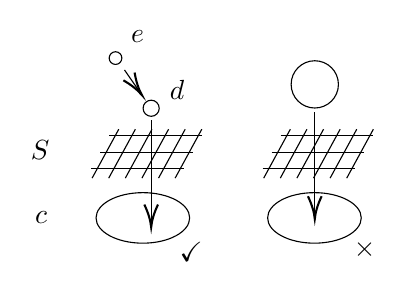
\begin{tikzpicture}[x=0.75pt,y=0.75pt,yscale=-1,xscale=1]
%uncomment if require: \path (0,300); %set diagram left start at 0, and has height of 300

%Shape: Ellipse [id:dp10401378338786049] 
\draw   (74,113.39) .. controls (74,106.67) and (84.1,101.22) .. (96.56,101.22) .. controls (109.01,101.22) and (119.11,106.67) .. (119.11,113.39) .. controls (119.11,120.11) and (109.01,125.56) .. (96.56,125.56) .. controls (84.1,125.56) and (74,120.11) .. (74,113.39) -- cycle ;
%Shape: Grid [id:dp09583060841478219] 
\draw  [draw opacity=0] (81.95,70.67) -- (126.56,70.67) -- (113.72,94.22) -- (69.11,94.22) -- cycle ; \draw   (84.95,70.67) -- (72.11,94.22)(92.95,70.67) -- (80.11,94.22)(100.95,70.67) -- (88.11,94.22)(108.95,70.67) -- (96.11,94.22)(116.95,70.67) -- (104.11,94.22)(124.95,70.67) -- (112.11,94.22) ; \draw   (80.31,73.67) -- (124.92,73.67)(75.95,81.67) -- (120.56,81.67)(71.59,89.67) -- (116.2,89.67) ; \draw    ;
%Shape: Circle [id:dp31189924819685966] 
\draw   (80.33,36.39) .. controls (80.33,34.7) and (81.7,33.33) .. (83.39,33.33) .. controls (85.08,33.33) and (86.44,34.7) .. (86.44,36.39) .. controls (86.44,38.08) and (85.08,39.44) .. (83.39,39.44) .. controls (81.7,39.44) and (80.33,38.08) .. (80.33,36.39) -- cycle ;
%Straight Lines [id:da12935033787340267] 
\draw    (87.72,42.11) -- (94.97,52.58) ;
\draw [shift={(96.11,54.22)}, rotate = 235.29] [color={rgb, 255:red, 0; green, 0; blue, 0 }  ][line width=0.75]    (10.93,-3.29) .. controls (6.95,-1.4) and (3.31,-0.3) .. (0,0) .. controls (3.31,0.3) and (6.95,1.4) .. (10.93,3.29)   ;
%Shape: Circle [id:dp7222065551952845] 
\draw   (96.67,60.56) .. controls (96.67,58.41) and (98.41,56.67) .. (100.56,56.67) .. controls (102.7,56.67) and (104.44,58.41) .. (104.44,60.56) .. controls (104.44,62.7) and (102.7,64.44) .. (100.56,64.44) .. controls (98.41,64.44) and (96.67,62.7) .. (96.67,60.56) -- cycle ;
%Straight Lines [id:da7276461675375434] 
\draw    (100.56,66.44) -- (100.56,115.89) ;
\draw [shift={(100.56,117.89)}, rotate = 270] [color={rgb, 255:red, 0; green, 0; blue, 0 }  ][line width=0.75]    (10.93,-3.29) .. controls (6.95,-1.4) and (3.31,-0.3) .. (0,0) .. controls (3.31,0.3) and (6.95,1.4) .. (10.93,3.29)   ;
%Shape: Ellipse [id:dp12697611260252684] 
\draw   (156.67,113.39) .. controls (156.67,106.67) and (166.77,101.22) .. (179.22,101.22) .. controls (191.68,101.22) and (201.78,106.67) .. (201.78,113.39) .. controls (201.78,120.11) and (191.68,125.56) .. (179.22,125.56) .. controls (166.77,125.56) and (156.67,120.11) .. (156.67,113.39) -- cycle ;
%Shape: Grid [id:dp9936460967678797] 
\draw  [draw opacity=0] (164.61,70.67) -- (209.22,70.67) -- (196.39,94.22) -- (151.78,94.22) -- cycle ; \draw   (167.61,70.67) -- (154.78,94.22)(175.61,70.67) -- (162.78,94.22)(183.61,70.67) -- (170.78,94.22)(191.61,70.67) -- (178.78,94.22)(199.61,70.67) -- (186.78,94.22)(207.61,70.67) -- (194.78,94.22) ; \draw   (162.98,73.67) -- (207.59,73.67)(158.62,81.67) -- (203.23,81.67)(154.26,89.67) -- (198.87,89.67) ; \draw    ;
%Shape: Circle [id:dp838751100400853] 
\draw   (168,49.06) .. controls (168,42.77) and (173.1,37.67) .. (179.39,37.67) .. controls (185.68,37.67) and (190.78,42.77) .. (190.78,49.06) .. controls (190.78,55.35) and (185.68,60.44) .. (179.39,60.44) .. controls (173.1,60.44) and (168,55.35) .. (168,49.06) -- cycle ;
%Straight Lines [id:da5932706956135338] 
\draw    (179.39,62.44) -- (179.39,111.89) ;
\draw [shift={(179.39,113.89)}, rotate = 270] [color={rgb, 255:red, 0; green, 0; blue, 0 }  ][line width=0.75]    (10.93,-3.29) .. controls (6.95,-1.4) and (3.31,-0.3) .. (0,0) .. controls (3.31,0.3) and (6.95,1.4) .. (10.93,3.29)   ;

% Text Node
\draw (43.33,109) node [anchor=north west][inner sep=0.75pt]   [align=left] {$\displaystyle c$};
% Text Node
\draw (41.33,75) node [anchor=north west][inner sep=0.75pt]   [align=left] {$\displaystyle S$};
% Text Node
\draw (113,123.67) node [anchor=north west][inner sep=0.75pt]   [align=left] {$\displaystyle \checkmark$};
% Text Node
\draw (197,123) node [anchor=north west][inner sep=0.75pt]   [align=left] {$\displaystyle \times $};
% Text Node
\draw (108.33,46) node [anchor=north west][inner sep=0.75pt]   [align=left] {$\displaystyle d$};
% Text Node
\draw (89.67,22) node [anchor=north west][inner sep=0.75pt]   [align=left] {$\displaystyle e$};


\end{tikzpicture}
    \end{center}

    % 这里, 我们认为指向 $c$ 的态射越复合就越小. 回忆环是一个对象的 $\mathsf {Ab}$-充实范畴, 那么其中的筛正是环的右理想; 筛的大小观念类似于 $p$-进度量下的整数越乘越小.

    一个筛越 ``细'', 能 ``通过'' 它的东西就越少, 这解释了\emph{细化}的含义.
\end{remark}

\begin{example}
	[label={sieve-from-cover}]
	{(覆盖产生筛)}
	设 $X$ 为拓扑空间, $\{U_i\}$ 是其中开集 $V$ 的一个开覆盖. 那么
	$$
	\big\{W\subset V \mid \exists i, W \subset U_i\big\}
	$$
	构成 $\operatorname{Open}(X)$ 中 $V$ 上的一个筛. 直观上每个 $U_i$ 是筛上的一个 ``洞'', 比它小的对象能 ``通过'' 这个筛.
\end{example}

\begin{prop}
	[label={sieve-and-subfunctor}]
    {(筛与子函子)}
    范畴 $\mathsf C$ 的对象 $c$ 上的筛自然地一一对应于 $\yo(c)$ 的子函子.
\end{prop}

\begin{proof}
    设 $S$ 是 $c$ 上的筛, 那么
    $$
    X(d) = \{f\colon d\to c \mid f\in S\} \subset \operatorname{Hom}_{\mathsf C}(d,c) = \yo(c)(d)
    $$
    构成 $\yo(c)$ 的子函子.
    设 $X \to \yo(c)$ 为子函子, 那么
    $$
    S=\big\{
        f \colon d\to c \mid f\in X(d)
    \big\}
    $$
    是 $c$ 上的筛. 很明显, 这两个对应是互逆的.
\end{proof}

\begin{remark}
    {}
    若将 $\widehat {\mathsf C}$ 的对象称作 $\mathsf C$ 的 ``广义对象'', 那么 $\yo(c)$ 的子函子可称作 $c$ 的 ``广义子对象''.

    $\mathsf C$ 的 ``广义对象'' $X$ 的子对象, 根据命题 \ref{subfunctor-description} 的描述, 也可视为 $X$ 上的 ``筛''.
\end{remark}

\begin{example}
	[label={sieve-from-cover-subfunctor}]
	{(覆盖产生的筛对应的子函子)}
	继续例 \ref{sieve-from-cover}, 设 $S$ 为覆盖 $\{U_i\}$ 生成的筛对应的 $\yo(V)$ 的子函子, 那么下图是余等化子.
	\begin{equation}
		\label{sieve-coeq}
		\begin{tikzcd}[ampersand replacement=\&]
			{\coprod_{i,j}\yo(U_i\cap U_j)} \& {\coprod_i \yo(U_i)} \& S
			\arrow[shift right, from=1-1, to=1-2]
			\arrow[shift left, from=1-1, to=1-2]
			\arrow[from=1-2, to=1-3]
		\end{tikzcd}
	\end{equation}
	这是因为, 由 $S$ 的定义, 对 $W\in\operatorname{Open}(X)$, 若存在 $i$, $W\subset U_i$ 则 $S(W)$ 是单元集; 否则 $S(W)$ 是空集. 由此可知下图是集合范畴中的余等化子.
	\[\begin{tikzcd}[ampersand replacement=\&, column sep=small]
		{\coprod_{i,j}\operatorname{Hom}_{\operatorname{Open}(X)}(W,U_i\cap U_j)} \& {\coprod_i \operatorname{Hom}_{\operatorname{Open}(X)}(W,U_i)} \& {S(W)}
		\arrow[shift right, from=1-1, to=1-2]
		\arrow[shift left, from=1-1, to=1-2]
		\arrow[from=1-2, to=1-3]
	\end{tikzcd}\]
	而预层的余极限是 ``逐点'' 的, 于是得 (\ref{sieve-coeq}).
	
	对 $X$ 上的任意预层 $F$, 以 $\operatorname{Hom}_{\operatorname{Presh}(X)}(-,F)$ 作用于 (\ref{sieve-coeq}), 可知下图是集合范畴中的等化子.
	\begin{equation}
		\begin{tikzcd}[ampersand replacement=\&]
			{\operatorname{Hom}_{\operatorname{Presh}(X)}(S,G)} \& {\prod_i G(U_i)} \& {\prod_{i,j}G(U_i\cap U_j)}
			\arrow[shift left, from=1-2, to=1-3]
			\arrow[shift right, from=1-2, to=1-3]
			\arrow[from=1-1, to=1-2]
		\end{tikzcd}
		\label{sieve-subfunctor-equalizer}
	\end{equation}
	因此态射集合 $\operatorname{Hom}_{\operatorname{Presh}(X)}(S,F)$ 表达了预层 $F$ 关于覆盖 $\{U_i\}$ 的下降资料 (descent data), 由覆盖 $\{U_i\}$ ``下降'' 到 $V$. 若 $F$ 为层, 就应该有 $$\operatorname{Hom}_{\operatorname{Presh}(X)}(S,F) \simeq F(V) \simeq \operatorname{Hom}_{\operatorname{Presh}(X)}(\yo(V),F).$$
\end{example}

\begin{example}
	[label={maximal-sieve}]
    {(极大筛)}
    所有指向 $c$ 的箭头的集合称为\emph{极大筛}, 也即最粗的筛.
    它对应 $\yo(c)$ 的子对象 $\yo(c)$ 自身 ($\yo(c)$ 到自身的恒等态射).
    注意, $c$ 上的一个筛是极大筛当且仅当它包含 $\operatorname{id}_c$.
\end{example}

现在我们给出命题 \ref{presheaf-category-subobject-classifier} 的证明.

\begin{proof}
    

    假设 $\widehat{\mathsf C}$ 中存在子对象分类子 $\Omega$, 那么由米田引理, 有自然同构
    $$
    \Omega(c) \simeq \operatorname{Hom}_{\widehat {\mathsf C}}(\yo(c),\Omega)
    \simeq \operatorname{Sub}_{\widehat {\mathsf C}}(\yo(c)),
    $$
    即
    $$
    \Omega(c) = \{\text{$c$ 上的筛}\},
    $$
    这便确定了函子 $\Omega$.
    下面验证这个函子确实满足 $\widehat{\mathsf C}$ 中子对象分类子的条件.

    定义态射 $\top\colon 1 \to \Omega,$
    对每个对象 $c$ 选出 $\Omega(c)= \operatorname{Sub}_{\widehat {\mathsf C}}(\yo(c))$
    中的子对象 $\yo(c)$ 自身, 也即 $c$ 上的极大筛.
    
    下面验证子对象分类子的条件. 设 $Y\to X$ 是 $\widehat{\mathsf C}$ 中的子对象.
    定义态射 $\chi \colon X \to \Omega$, 将 $x\in X(c)$ 对应到 $c$ 上的筛
    $$
    \chi(x) = \big\{f \colon d \to c \mid X(f)(x) \in Y(d)\big\}.
    $$
    注意 $\chi(x)$ 是极大筛当且仅当 $\operatorname{id}_c \in \chi(x)$, 也即 $x \in Y(c)$,
    所以子对象 $Y\to X$ 是如下的拉回.
    % https://q.uiver.app/#q=WzAsNCxbMCwxLCJYIl0sWzEsMSwiXFxPbWVnYSJdLFsxLDAsIjEiXSxbMCwwLCJZIl0sWzMsMF0sWzAsMSwiXFxjaGkiLDJdLFsyLDEsIlxcdG9wIl0sWzMsMl1d
    \[\begin{tikzcd}[ampersand replacement=\&]
    	Y \& 1 \\
    	X \& \Omega
    	\arrow[from=1-1, to=2-1]
    	\arrow["\chi"', from=2-1, to=2-2]
    	\arrow["\top", from=1-2, to=2-2]
    	\arrow[from=1-1, to=1-2]
    \end{tikzcd}\]
\end{proof}

综合上述论证, 我们得到
\begin{prop}{}
    $\widehat {\mathsf C}$ 是一个\topos{}.
\end{prop}

\begin{example}
    {($G$-集)}
    例 \ref{G-set-presheaf-category} 介绍了 $G$-集范畴, 即 $\mathsf BG$ 上的预层范畴. 由于 $\mathsf BG$ 只有一个对象且态射均为自同构,
    其上仅有两个筛, 空集与极大筛.
    
    因此, $G$-集范畴的子对象分类子 $\Omega$ 是二元集合 $\{\top,\bot\}$, 其上带有 $G$ 的平凡作用.
    事实上, 一个 $G$-集 $X$ 的子对象 $Y$ 是其中 $G$-作用下封闭的子集. 其对应的特征函数 $X\to\{\top,\bot\}$ 就是子集 $Y$ 的特征函数.
\end{example}


\section{层与景}

拓扑空间上的\emph{层}是满足 ``粘合'' 条件的预层; 一个开集上的截面\footnote{预层 $F$ 在 $U$ 上的\emph{截面} (section) 就是指 $F(U)$ 的元素. 这个术语来自于几何.}可由这个开集的任何一个覆盖上一族相容的截面唯一决定.

\begin{definition}
    {(拓扑空间上的层)}
    拓扑空间 $X$ 上的\emph{层} (sheaf) 是满足如下条件的预层 $F$:
    对任意开集 $U\subset X$, 任意覆盖 $U = \bigcup_i U_i$,
    以及任意一组相容的元素 \makebox{$(s_i \in F(U_i))_{i\in I}$},
    存在唯一的 $s\in F(U)$
    满足 $s|_{U_i} = s_i\,\forall i\in I$.
    其中相容是指
    \begin{equation}
        s_i|_{U_i\cap U_j} = s_j|_{U_i\cap U_j}\,(\forall i,j \in I),
        \label{sheaf-condition}
    \end{equation}
\end{definition}

Grothendieck 意识到, 层的概念所需的关键信息是一个对象 $U$ 何时被一族进入 $U$ 的态射 (甚至不一定是 $U$ 的子对象) 所\emph{覆盖}.

\subsection{覆盖与 Grothendieck 覆盖}
\begin{definition}{(覆盖结构)}
    设范畴 $\mathsf C$ 具有拉回.
    $\mathsf C$ 上的一个\emph{覆盖结构} (coverage) $T$ 是对每个对象 $c$ 指定一个集合 $T(c)$, 其元素为态射族 $\{f_i \colon c_i \to c\}_{i\in I}$, 称为 $c$ 的 $T$-\emph{覆盖族} (covering family), 满足\emph{拉回下的稳定性}, 或称\emph{基变换下的稳定性}:
    \begin{center}
    	若 $\{f_i \colon c_i \to c\}_{i\in I}\in T(c)$, $g \colon d \to c$,
    	则 $\{g^*(f_i) \colon d_i \to d\}_{i\in I}\in T(d)$.
    \end{center}
    
    
    %带有覆盖结构的范畴 $(\mathsf C,T)$ 称为\emph{景} (site).
\end{definition}

对于拓扑空间的开集范畴, 拉回下的稳定性相当于若一族开集覆盖了 $U$, 那么它们也覆盖了 $U$ 的任何子集.

\begin{remark}
    {}
    当 $\mathsf C$ 不存在拉回时, ``拉回下的稳定性'' 可改为: 若 $\{f_i \colon c_i \to c\}_{i\in I}\in T(c)$, $g \colon d \to c$,
    则存在 $\{h_j \colon d_j \to d\}_{j\in J}\in T(d)$,
    使得每个 $gh_j$ 都穿过某个 $f_i$.
\end{remark}

%\begin{remark}{}
%    上面定义的覆盖结构有时也称为范畴上的 \emph{Grothendieck 拓扑}, 但这个词的含义有时要窄一些.
%\end{remark}

\begin{definition}
	[label={sheaf-condition}]
	{(层条件)}
	设 $T$ 是范畴 $\mathsf C$ 上的覆盖结构. 对于 $\mathsf C$ 上的预层 $F$, 称 $F$ 满足关于 $T$ 的\emph{层条件}是指:
	对 $\mathsf C$ 的任意对象 $c$, 任意 $\{f_i\colon c_i\to c\}_{i\in I}\in T(c)$,
	以及任意一组相容的元素 $(s_i\in F(c_i))_{i\in I}$,
	存在唯一的 $s\in F(c)$ 满足 $F(f_i)(s)=s_i\,\forall i\in I$.
	其中, 一组元素 $(s_i\in F(c_i))_{i\in I}$ \emph{相容}是指 对任意态射 $f\colon d \to c_i$, $g\colon d \to c_j$, 有 $F(f)(s_i) = F(g)(s_j) \in F(d)$.
	
	在 $\mathsf C$ 具有拉回的条件下, 层条件可简洁地表述为如下等化子,
	% https://q.uiver.app/#q=WzAsMyxbMCwwLCJGKGMpIl0sWzEsMCwiXFxwcm9kX3tpfSBGKGNfaSkiXSxbMiwwLCJcXHByb2Rfe2ksan0gRihjX2lcXHRpbWVzX2MgY19qKSJdLFsxLDIsIiIsMCx7Im9mZnNldCI6LTF9XSxbMSwyLCIiLDIseyJvZmZzZXQiOjF9XSxbMCwxXV0=
	\[\begin{tikzcd}[ampersand replacement=\&]
		{F(c)} \& {\prod_{i} F(c_i)} \& {\prod_{i,j} F(c_i\times_c c_j)}
		\arrow[shift left, from=1-2, to=1-3]
		\arrow[shift right, from=1-2, to=1-3]
		\arrow[from=1-1, to=1-2]
	\end{tikzcd}\]
	
	设 $S\to \yo(c)$ 是 $\{f_i\colon c_i\to c\}_{i\in I}$ 生成的筛对应的子函子 (命题 \ref{sieve-and-subfunctor}), 那么一组相容的元素等同于自然变换 $S\to F$,	从而 $F$ 的层条件等价于对所有这样的 $S$, 自然变换 $S\to F$ 唯一地穿过 $\yo(c)$, 也即如下映射是同构.
	$$
	\operatorname{Hom}_{\widehat {\mathsf C}}(\yo(c),F) \to \operatorname{Hom}_{\widehat {\mathsf C}}(S,F)
	$$
	对比例 \ref{sieve-from-cover-subfunctor} 中的式 (\ref{sieve-subfunctor-equalizer}).
\end{definition}

\begin{definition}
	{(层范畴)}
	设 $T$ 是范畴 $\mathsf C$ 上的覆盖结构. 定义\emph{层范畴} $\operatorname{Sh}(\mathsf C,T)$ 为 $\widehat {\mathsf C}$ 中满足关于 $T$ 的层条件的预层构成的满子范畴.
\end{definition}

设 $T$ 是范畴 $\mathsf C$ 上的覆盖结构. 所有 $T$ 中的覆盖族生成的筛 (定义 \ref{sieve}) 定义了一个新的覆盖结构 $\overline{T}$; 可以证明 $T$ 的层条件等价于 $\overline{T}$ 上的层条件. 这就是说, 对于一个覆盖结构, 我们总可以设其中的覆盖族都是筛, 而不改变层条件.
这样的覆盖结构称为\emph{筛覆盖结构} (sifted coverage). %后面我们将默认讨论筛覆盖.

% Grothendieck 最初考虑的覆盖在上面定义的 ``覆盖结构'' 之上附加了更多条件.

``覆盖结构'' 是从 \emph{Grothendieck 覆盖}的概念中分离出的一个比较重要的条件. Grothendieck 覆盖的完整概念 (用筛覆盖叙述) 如下.

\begin{definition}
	[label={Grothendieck-topology}]
	{(Grothendieck 覆盖)}
	范畴 $\mathsf C$ 的 \emph{Grothendieck 覆盖} (或 Grothendieck 拓扑) 是满足如下条件的筛覆盖 $T$:
	\begin{itemize}
		\item 任和对象 $c$ 上的极大筛 (定义 \ref{maximal-sieve}) 构成 $c$ 的 $T$-覆盖族;
		\item (传递性) 若 $R$ 是 $c$ 的 $T$-覆盖族, $S$ 是 $c$ 上的另一个筛, 使得对任意 $(f\colon d\to c)\in R$, 都有 $f^*S$ 是 $d$ 的 $T$-覆盖族, 那么 $S$ 也是 $c$ 的 $T$-覆盖族.
	\end{itemize}
\end{definition}

对于拓扑空间的开集范畴, ``极大筛是覆盖'' 相当于任何开集 $U$ 都覆盖了自己; 传递性相当于若一族开集覆盖了 $U$ 的每个局部, 那么它们也覆盖了 $U$.

%\begin{definition}
%	{(Grothendieck 覆盖的基)}
%	
%\end{definition}

覆盖可以生成 Grothendieck 覆盖, 就像拓扑基生成拓扑一样:

\begin{definition}
	{(覆盖结构生成的 Grothendieck 覆盖)}
	覆盖结构 $T$ \emph{生成的 Grothendieck 覆盖}是包含 $T$ 和所有极大筛且满足传递性的最小的一族筛.
	
%	等价地, 覆盖结构 $T$ 生成的 Grothendieck 覆盖是每个对象 $c$ 上满足如下条件的筛 $S$:
%	\begin{itemize}
%		\item 对任意态射 $f\colon b\to c$ 与 $b$ 上的任意筛 $R$,
%		
%	\end{itemize}
\end{definition}

%\todo{澄清 Grothendieck 拓扑与覆盖的关系}

%将拓扑空间上层的定义稍微修改, 就得到景上的层的定义.
%\begin{definition}
%    [label={sheaf-on-site}]
%    {(景上的层)}
%    设 $(\mathsf C,T)$ 是一个景. 其上的\emph{层}是满足如下条件的预层 $F$:
%    对任意 $T$-覆盖族 $\{f_i \colon c_i \to c\}_{i\in I}$,
%    以及任意一组相容的元素 \makebox{$(s_i \in F(c_i))_{i\in I}$},
%    存在唯一的 $s\in F(c)$
%    满足 $F(f_i)(s) = s_i\,\forall i\in I$.
%    其中相容是指,
%    对任意态射 $f\colon d \to c_i$, $g\colon d \to c_j$,
%    有 $F(f)(s_i) = F(g)(s_j) \in F(d)$.
%
%    定义景 $(\mathsf C,T)$ 上的层范畴 $\operatorname{Sh}(\mathsf C,T)$ 为层在 $\widehat {\mathsf C}$ 中构成的满子范畴.
%\end{definition}

事实上, 覆盖与 Grothendieck 覆盖有如下的关系.

\begin{prop}
	{}
	对范畴 $\mathsf C$ 上任一覆盖 $T$, \emph{存在唯一的 Grothendieck 覆盖} $J$ 使得 $(\mathsf C,T)$ 上的层与 $(\mathsf C,J)$ 上的层相同.
\end{prop}

\begin{definition}
	{(景)}
	带有覆盖结构或 Grothendieck 覆盖的范畴称为\emph{景}.
\end{definition}

\subsection{常见的景}

% 正如环中一族元素可以生成一个右理想, 范畴 $\mathsf C$ 中一族指向 $U$ 的箭头也可以生成一个筛. 容易看到, 将覆盖族替换为生成的筛, 不影响层的概念 (正如将环中的一族元素替换为其生成的理想, 不影响对应谱上的闭集一样). 因此我们不妨考虑仅由筛构成的覆盖结构.

\begin{example}
    {}
    每个范畴 $\mathsf C$ 都构成一个平凡的景, 其上的覆盖结构是空的,
    也即没有覆盖. 由定义, 这个景上的层是 $\mathsf C$ 上的预层.
\end{example}

\begin{example}
    [label={topological-space-as-site}]
    {}
    拓扑空间 $X$ 的开集范畴 $\operatorname{Open}(X)$ 构成一个景, 其上的覆盖结构就是开覆盖.
\end{example}

%\todo{解释景的小性}

\begin{example}
    {}
    拓扑空间范畴 $\mathsf {Top}$ 上有一个覆盖结构, 即开覆盖. %然而 $\mathsf {Top}$ 不是小范畴.
\end{example}

\begin{example}
	[label={locale-as-site}]
    {(位象)}
    % 定义\emph{位象}是一个偏序集 $A$, 存在有限交与任意并 (若将偏序集视为范畴, 这个条件就是说存在有限极限与任意余极限), 且满足分配律
    % $$a \wedge \bigvee_{i\in I} b_i = \bigvee_{i\in I} (a\wedge b_i)\,(\forall a,b_i\in A),$$
    % 其中 $I$ 是任意集合.
    % 位象的态射 $A\to B$ 是偏序集的\emph{反向}态射 $B\to A$ (想象开集的拉回), 保持有限交与任意并.
    
    对于位象 $A$, 将其视为范畴, 我们定义 $A$ 上的覆盖结构:
    当一族态射 $\{U_i \to U\}_{i\in I}$ 满足 $U = \bigvee_{i\in I} U_i$ 时, 称其为覆盖族.
    由此, 每个位象都是一个景.
\end{example}

\begin{example}
    [label={cartsp-site}]
    {(欧氏空间景)}
    考虑范畴 $\mathsf C$, 其中的对象为 $\mathbb{R}^0,\mathbb{R}^1,\mathbb{R}^2,\cdots$,
    态射为光滑映射.
    称 $\mathbb{R}^n$ 的开覆盖 $\bigcup_i U_i$ 为 \emph{好覆盖} (good cover) 是指 $U_i$ 以及任意有限个 $U_i$ 的交都同胚于 $\mathbb{R}^n$.
    这给出了范畴 $\mathsf C$ 上的一个覆盖结构, 称之为欧氏空间景.
    欧氏空间景上的层称作\emph{光滑空间} (smooth space).
    光滑空间是流形的推广, 是\emph{广义微分几何} (diffeology) 的研究对象.
\end{example}

\begin{example}
    [label={zariski-site}]
    {(Zariski 景)}
    %固定环 $k$,
    考虑\emph{有限表现} (finitely presented) 环 (形如 $\mathbb{Z}[x_1,\cdots,x_n]/(f_1,\cdots,f_m)$ 的环) 的范畴 $\mathsf {Ring}_{\text{fp}}$. 这是一个小范畴\footnotemark.
    我们考虑其对偶范畴 $\mathsf {Ring}_{\text{fp}}^{\op}$, 也即仿射概形的范畴.
    对于环 $A$, 我们记 $\operatorname{Spec} A \in \mathsf {Ring}_{\text{fp}}^{\op}$ 为 $A$ 在对偶范畴中的化身.

    回忆, Zariski 拓扑的标准开集 (但不一定是全部的开集) 形如 $\operatorname{Spec} A[f^{-1}] \to \operatorname{Spec}A$, 也即局部化的环同态 $A \to A[f^{-1}]$. 若 $n$ 个元素 $f_1,\cdots,f_n \in A$ 生成了单位理想 $(1)$ ($f_1,\cdots,f_n$ 构成了 $\operatorname{Spec}A$ 上的 ``单位分解''),
    则 $\operatorname{Spec}A[f^{-1}] \to \operatorname{Spec}A$ 构成开覆盖. 这定义了 $\mathsf {Ring}_{\text{fp}}^{\op}$ 上的一个覆盖结构, 这便是 \emph{Zariski 景}.
    Zariski 景是\emph{综合代数几何} (synthetic algebraic geometry) 的基础.

    Zariski 景上的\emph{结构层} (structure sheaf) 是遗忘函子 $\mathsf{Ring}_{\text{fp}} \to \mathsf{Set}$.
    \todo{这个层的意义}
\end{example}

\footnotetext{严格地说, 它是本质小 (essentially small) 范畴, 也即它的对象模掉同构之后构成一个集合.}

\subsection{Lawvere--Tierney 拓扑}

回忆筛覆盖结构就是 ``函子性地'' 指定了每个对象上的一些筛, 而 $\widehat {\mathsf C}$ 的子对象分类子 $\Omega$ 是函子 $\Omega(c) = \{\text{$c$ 上的筛}\}$. 因此

\begin{prop}
	{}
	设 $\mathsf C$ 为范畴, 函数 $J$ 给每个对象 $c$ 赋予一族筛 $J(c)$, 那么 $J$ 满足传递性 (定义 \ref{Grothendieck-topology}) 当且仅当 $J$ 是 $\widehat {\mathsf C}$ 的子对象分类器 $\Omega$ 的子函子.
\end{prop}

而由子对象分类子的定义, 子函子 $J$ 进一步对应一个态射 $j\colon \Omega \to \Omega$.
这个态射可以承载一个覆盖结构的所有信息.
具体地, 对 $\mathsf C$ 的对象 $c$,
$$
j_c(S) = \{f\colon d\to c\mid f^*S \in J(d)\}.
$$

\todo{}

\subsection{层范畴中的子对象}

回忆预层范畴 $\widehat {\mathsf C}$ 的子对象分类子为 $\Omega(c) = \{\text{$c$ 上的筛}\}$, 因为 $\yo(c)$ 的子对象等同于 $c$ 上的筛. 固定范畴 $\mathsf C$ 上的 Grothendieck 拓扑 $J$, 本小节研究 $\operatorname{Sh}(\mathsf C,J)$ 的子对象 (分类子).

% 由定义, $\operatorname{Sh}(\mathsf C,J)$ 是 $\widehat {\mathsf C}$ 的满子范畴

层范畴中的子对象放在预层范畴中仍是子对象. 这不是显然的, 我们采用如下的思路来证明这个事实.
%注意到在任何范畴中态射 $f\colon X\to Y$ 是单射当且仅当
%% https://q.uiver.app/#q=WzAsNCxbMCwwLCJYIl0sWzEsMCwiWCJdLFswLDEsIlgiXSxbMSwxLCJZIl0sWzAsMSwiXFxvcGVyYXRvcm5hbWV7aWR9X1giXSxbMSwzLCJmIl0sWzAsMiwiXFxvcGVyYXRvcm5hbWV7aWR9X1giLDJdLFsyLDMsImYiLDJdXQ==
%$$\begin{tikzcd}[ampersand replacement=\&,sep=scriptsize]
%	X \& X \\
%	X \& Y
%	\arrow["{\operatorname{id}_X}", from=1-1, to=1-2]
%	\arrow["f", from=1-2, to=2-2]
%	\arrow["{\operatorname{id}_X}"', from=1-1, to=2-1]
%	\arrow["f"', from=2-1, to=2-2]
%\end{tikzcd}$$
%是拉回\footnote{可直接验证, 也可考虑俯范畴 $\mathsf C/Y$ 中的子终对象, 例 \ref{subterminal-of-slice-category}},
由单射的拉回刻画 (命题 \ref{mono-epi-pullback-pushout}), 我们只需证明\emph{层的拉回也是预层的拉回}. %一般地有如下命题.

\begin{prop}
	{}
	在预层的拉回图
	% https://q.uiver.app/#q=WzAsNCxbMCwxLCJYIl0sWzEsMSwiWSJdLFsxLDAsIloiXSxbMCwwLCJXIl0sWzAsMV0sWzIsMV0sWzMsMF0sWzMsMl1d
	$\begin{tikzcd}[ampersand replacement=\&,sep=1em]
		W \& Z \\
		X \& Y
		\arrow[from=2-1, to=2-2]
		\arrow[from=1-2, to=2-2]
		\arrow[from=1-1, to=2-1]
		\arrow[from=1-1, to=1-2]
	\end{tikzcd}$
	中, 若 $X,Y,Z$ 为层, 则 $W$ 为层.
\end{prop}

\begin{proof}
	设 $S\in J(c)$ 是任意覆盖筛, 视为 $\yo(c)$ 的子函子.
	分别以
	$\operatorname{Hom}_{\widehat {\mathsf C}}(\yo(c),-)$,
	$\operatorname{Hom}_{\widehat {\mathsf C}}(S,-)$
	作用于上述拉回图
	(注意这类函子保持极限),
	得到立方体
	% https://q.uiver.app/#q=WzAsOCxbMSwxLCJcXG9wZXJhdG9ybmFtZXtIb219KFxceW8oYyksWCkiXSxbMywxLCJcXG9wZXJhdG9ybmFtZXtIb219KFxceW8oYyksWSkiXSxbMiwwLCJcXG9wZXJhdG9ybmFtZXtIb219KFxceW8oYyksWikiXSxbMCwwLCJcXG9wZXJhdG9ybmFtZXtIb219KFxceW8oYyksVykiXSxbMSwzLCJcXG9wZXJhdG9ybmFtZXtIb219KFMsWCkiXSxbMywzLCJcXG9wZXJhdG9ybmFtZXtIb219KFMsWSkiXSxbMiwyLCJcXG9wZXJhdG9ybmFtZXtIb219KFMsWikiXSxbMCwyLCJcXG9wZXJhdG9ybmFtZXtIb219KFMsVykiXSxbMCwxXSxbMiwxXSxbMywwXSxbMywyXSxbNyw0XSxbNCw1XSxbNyw2XSxbNiw1XSxbMyw3XSxbMCw0XSxbMiw2XSxbMSw1XV0=
	\[\begin{tikzcd}[ampersand replacement=\&,column sep=-2em,row sep=small]
		{\operatorname{Hom}(\yo(c),W)} \&\& {\operatorname{Hom}(\yo(c),Z)} \\
		\& {\operatorname{Hom}(\yo(c),X)} \&\& {\operatorname{Hom}(\yo(c),Y)} \\
		{\operatorname{Hom}(S,W)} \&\& {\operatorname{Hom}(S,Z)} \\
		\& {\operatorname{Hom}(S,X)} \&\& {\operatorname{Hom}(S,Y),}
		\arrow[from=2-2, to=2-4]
		\arrow[from=1-3, to=2-4]
		\arrow[from=1-1, to=2-2]
		\arrow[from=1-1, to=1-3]
		\arrow[from=3-1, to=4-2]
		\arrow[from=4-2, to=4-4]
		\arrow[from=3-1, to=3-3]
		\arrow[from=3-3, to=4-4]
		\arrow[from=1-1, to=3-1]
		\arrow[from=2-2, to=4-2]
		\arrow[from=1-3, to=3-3]
		\arrow[from=2-4, to=4-4]
	\end{tikzcd}\]
	其上下两面均为拉回图.
	由层条件的等价表述 (定义 \ref{sheaf-condition}),
	立方体的竖直方向箭头有三个为同构, 从而第四个也为同构, 这证明了 $W$ 是层.
\end{proof}

上述论证中的拉回图可替换为任何极限. 因此有

\begin{prop}
	{}
	层范畴 $\operatorname{Sh}(\mathsf C,J)$ 存在任意极限, 且极限等同于作为预层的极限.
\end{prop}
%
%\begin{proof}
%	设 $X = \lim _i X_i$ 是预层的极限, 而每个 $X_i$ 是层, 我们证明 $X$ 是层.
%\end{proof}

回到正题, 我们证明了

\begin{prop}
	{}
	层范畴中的子对象即是预层范畴中的子对象.
\end{prop}

假设 $\operatorname{Sh}(\mathsf C,J)$ 有子对象分类子 $\Omega_J$,
那么 $\Omega_J(c)$ 等同于 $\yo(c)$

\begin{prop}
	{}
	设 $F$ 是 $(\mathsf C,J)$ 上的层.
	
\end{prop}

\todo{J-closed}

\subsection{层范畴中的指数对象}



\section{拓扑空间上的层与平展空间}

在本节中我们暂时将考虑的范围限制在拓扑空间.

固定拓扑空间 $X$. 称俯范畴 (定义 \ref{over-category}) $\mathsf {Top}/X$ 的对象, 即映射 $p \colon Y \to X$, 为 $X$ \emph{上的空间} 或 $X$ 上的丛\footnote{这里的丛不一定是所谓纤维丛.}.

\begin{definition}
    {(丛的截面)}
    对于 $X$ 上的空间 $p \colon Y\to X$, 定义其在开集 $U\subset X$ 上的\emph{截面}的集合为
    $$
    \Gamma_p(U)=
    \big\{
        s \colon U \to Y \mid ps=i\colon U \to X
    \big\}.
    $$
    对于子开集 $V\subset U$, 有限制映射 $\operatorname{res}\colon \Gamma_p(U) \to \Gamma_p(V)$, 这使得 $\Gamma_p$ 成为 $X$ 上的预层.
\end{definition}

\begin{propdef}
    {(截面层)}
    对于 $X$ 上的空间 $p \colon Y\to X$, 上面定义的 $\Gamma_p$ 构成 $X$ 上的一个层, 称为丛 $p$ 的\emph{截面层}.
    
    截面层给出了函子
    $$\Gamma \colon \mathsf {Top}/X \to \operatorname{Presh}(X).$$
\end{propdef}

我们将证明每个层都是某个丛的截面层, 其中要用到\emph{芽} (germ).
芽的概念来自函数芽: 两个函数在一点处有相同的芽, 是指它们在这点的某个邻域上取值相等. 这个概念可自然地定义在一般的预层上.

\begin{definition}
	[label={germ-and-stalk}]
	{(芽, 茎)}
    设 $F$ 是拓扑空间 $X$ 上的预层. 考虑在一点 $x\in X$ 附近的局部截面 (也即 $x$ 的邻域上的截面) 的如下等价关系 $\sim$: 对于 $s\in F(U),t\in F(V)$, 若 $s|_{U\cap V}=t|_{U\cap V}$, 则 $s\sim t$. 称这个关系下的一个等价类为 $F$ 在 $x$ 处的一个\emph{芽}, 记截面 $s$ 所属的等价类为 $s_x$.
    
    称 $F$ 在 $x$ 处芽的集合为\emph{茎} (stalk) $F_x$.
    使用范畴语言, 茎是如下的余极限:
    $$
    F_x = \operatorname{colim}_{x\in U}F(U).
    $$
\end{definition}

由预层出发可构造一个丛, 即所谓平展空间.

\begin{definition}
    {(平展映射)}
    对于拓扑空间的映射 $f \colon Y \to X$,
    若对任意 $y\in Y$ 都存在 $y$ 的邻域 $V$ 与 $f(y)$ 的邻域 $U$ 使得 $f|_V \colon V \to U$ 为同胚,
    则称 $f$ 为\emph{平展} (étale) 映射, 又称局部同胚.
    到空间 $X$ 的平展态射构成的 $\mathsf {Top}/X$ 的满子范畴记为 $\mathsf {Et}(X)$.
\end{definition}

\begin{propdef}
	[label={espace-etale}]
    {(平展空间)}
    设 $F$ 是拓扑空间 $X$ 上的预层. 定义预层 $F$ 的\emph{平展空间} (espace étalé)
    $p \colon \Lambda_F \to X$ 如下.

    空间 $\Lambda_F$ 作为集合是无交并
    $$
    \Lambda_F = \coprod_{x\in X} F_x,
    $$
    映射 $p \colon \Lambda_F \to X$ 为投影, 将 $F_x$ 的元素映射到 $x$.
    
    对任意截面 $s\in F(U)$, 定义函数 $\dot{s} \colon U \to \Lambda_F$, $x\mapsto s_x$; 即 $\dot s$ 是取 $s$ 每个点处的截面芽得到的函数.
    定义 $\Lambda_F$ 上的拓扑为所有形如 $\dot{s}(U)$ 的集合生成的拓扑.
    那么平展空间是平展态射, 且定义了函子
    $$
    \Lambda \colon \operatorname{Presh}(X) \to \mathsf {Top}/X.
    $$
\end{propdef}

平展空间的一个重要性质是

\begin{prop}
    [label={etale-section-adjoint}]
    {(平展空间--截面伴随)}
    对于拓扑空间 $X$, $\operatorname{Presh}(X)$ 与 $\mathsf {Top}/X$ 之间存在伴随
    % https://q.uiver.app/#q=WzAsMixbMSwwLCJcXG1hdGhzZiB7VG9wfS9YIl0sWzAsMCwiXFxvcGVyYXRvcm5hbWV7UHJlc2h9KFgpIl0sWzAsMSwiXFxHYW1tYSIsMCx7Im9mZnNldCI6LTJ9XSxbMSwwLCJcXExhbWJkYSIsMCx7Im9mZnNldCI6LTJ9XSxbMywyLCIiLDAseyJsZXZlbCI6MSwic3R5bGUiOnsibmFtZSI6ImFkanVuY3Rpb24ifX1dXQ==
    \[\begin{tikzcd}[ampersand replacement=\&]
    	{\operatorname{Presh}(X)} \& {\mathsf {Top}/X.}
    	\arrow[""{name=0, anchor=center, inner sep=0}, "\Gamma", shift left=2, from=1-2, to=1-1]
    	\arrow[""{name=1, anchor=center, inner sep=0}, "\Lambda", shift left=2, from=1-1, to=1-2]
    	\arrow["\dashv"{anchor=center, rotate=-90}, draw=none, from=1, to=0]
    \end{tikzcd}\]
\end{prop}

\begin{proof}
    我们构造单位与余单位
    $$\eta \colon \operatorname{id}_{\operatorname{Presh}(X)} \to \Gamma\Lambda,\quad \epsilon \colon \Lambda\Gamma \to \operatorname{id}_{\mathsf {Top}/X}.$$

	\paragraph{单位}
	对于 $X$ 上的预层 $F$, 在 $\Lambda_F$ 的定义中已经给出一个映射
	$$
		\eta_F(U) \colon F(U) \to \Gamma\Lambda_F (U),\quad
		s\mapsto \dot s.
	$$
	这构成一个预层态射
	$\eta_F \colon F \to \Gamma\Lambda_F$. %$\eta$ 将一个预层的截面对应到其平展空间的截面芽.
	\paragraph{余单位}
	对 $X$ 上的空间 $p \colon Y \to X$,
	回忆 $\Lambda \Gamma_p$ 的一个元素可表示为一个芽 $s_x$, 其中
	$s\in \Gamma_p (U)$, $U$ 为 $x$ 的邻域.
	我们别无他选, 只能定义映射
	$$
		\epsilon_p \colon \Lambda \Gamma_p \to Y,\quad
		s_x \mapsto s(x).
	$$
	这构成了平展空间的态射. %$\epsilon$ 将一个平展空间的截面芽投影到其自身的点.
	
    下面考虑两个复合
    $$
    \Gamma \overset{\eta \Gamma}{\longrightarrow} \Gamma\Lambda\Gamma \overset{\Gamma\epsilon}{\longrightarrow} \Gamma,
    \quad
    \Lambda \overset{\Lambda\eta}{\longrightarrow} \Lambda\Gamma\Lambda \overset{\epsilon\Lambda}{\longrightarrow} \Lambda.
    $$

	\paragraph{第一个复合}
	对任意平展映射 $p \colon Y \to X$ 与截面 $s \in \Gamma_p(U)$,
    由 $\eta$ 的定义有
    $(\eta\Gamma)_p (U)(s) = \dot s \in \Gamma\Lambda\Gamma_p(U)$,
    而由 $\epsilon$ 的定义,
    $(\Gamma\epsilon)_p(U)(\dot s) = s$.
    因此第一个复合是恒等.

    \paragraph{第二个复合}
    对 $X$ 上的任一预层 $F$
    与芽 $s_x\in \Lambda_F$,
    $(\Lambda\eta)_F(s_x) = (\dot s)_x \in \Lambda\Gamma\Lambda_F$,
    而 $(\epsilon\Lambda)_F((\dot s)_x) = (\dot s)(x) = s_x$.
    因此第二个复合是恒等.
    
    ~\\
    
    综上, 我们完成了这一对伴随的证明.
    %\todo{第二个复合的计算}
\end{proof}

\begin{prop}
    {}
    命题 \ref{etale-section-adjoint} 中的伴随限制为满子范畴的等价
    $$
    \operatorname{Sh}(X) \simeq \mathsf {Et}(X).
    $$
\end{prop}

\begin{proof}
	注意到,
	\begin{itemize}
		\item $X$ 上的预层 $F$ 是层当且仅当 $\eta_F\colon F \to \Gamma\Lambda_F$ 是同构.
		\item $X$ 上的空间 $p\colon Y \to X$ 是平展空间当且仅当 $\epsilon_p \colon \Lambda\Gamma_p \to Y$ 是同构.
	\end{itemize}
	
	于是, 这个命题化为纯粹范畴论的问题. 见命题 \ref{adjoint-full-subcategory-equivalence}.
\end{proof}

\subsection{层\topos{}}

\begin{propdef}
	{}
	设 $(\mathsf C,T)$ 是景, 那么 $\operatorname{Sh}(\mathsf C,T)$ 为\topos{},
	称这样的\topos{}为 \emph{Grothendieck \topos{}}.
\end{propdef}

首先, $\operatorname{Sh}(\mathsf C,T)$ 中的 (小) 极限就是预层的极限, 即逐点极限;
换言之, 满足层条件的预层关于极限封闭.

回忆 $\mathsf C$ 上预层范畴的子对象分类子 $\Omega$ 为 $\Omega(c) = \{\text{$c$ 上的筛}\}$.

对于 $c$ 上的筛 $S$, 若以下条件成立则称其 $T$-封闭:
对任意态射 $f \colon d \to c$,
若存在 $T$-覆盖族 $\{g_i \colon d_i \to d \mid i\in I\}$
使得每个 $fg_i$ 都属于 $S$, 则 $f$ 属于 $S$.

\todo{证明}

\begin{remark}
	{(``小'' \topos{}与 ``大'' \topos{})}
	粗略地说, 层以及层\topos{}有两种不同的风味.
	一种是\emph{一个空间}上的层 (如例 \ref{topological-space-as-site}),
	一种是\emph{一类空间的范畴}上的层 (如例 \ref{cartsp-site}).
	Grothendieck 称前者的\topos{}为\emph{小\topos{}} (petit topos),
	后者的\topos{}为\emph{大\topos{}} (gros topos).
\end{remark}

\topos{}可以视为 ``空间'' 概念的推广, 一个重要原因就是由层\topos{}可以重构出这个 ``空间''.

考虑一个位象 $X$. 回忆 $\operatorname{Sh}(X)$ 的终对象 $1$ 是在所有开子集上取值为 $1$ 的层, 故 $\operatorname{Sh}(X)$ 的子终对象 (定义 \ref{subterminal-object-definition}) 是取值为 $0$ 或 $1$ 的层. 由层条件, 当一个子终层 ($\operatorname{Sh}(X)$ 的子终对象) 在若干开子集 $U_i\in\mathcal O(X)$ 上取值为 $1$ 时, 它在 $\bigvee_i U_i$ 上取值也为 $1$; 因此存在这个层取值为 $1$ 的最大开子集. 这证明了如下的 ``重构'' 定理:

\begin{prop}
	{(由层\topos{}重构位象)}
	位象 $X$ 上的层\topos{} $\operatorname{Sh}(X)$ 的子终对象一一对应于 $X$ 的开子集. 换言之, $X$ 作为\fm{} 同构于 $\operatorname{Sh}(X)$ 的子终对象的格:
	$$
	X \simeq \operatorname{Sub}_{\operatorname{Sh}(X)}(1).
	$$
\end{prop}

因此, SGA 4 \cite{SGA4} 作了如下定义.

\begin{definition}
	[label={ouvert}]
	{(\topos{}的开子空间)}
	一个\topos{}中的子终对象称为其\emph{开子空间} (法 ouvert).
\end{definition}

\subsection{层化}

设 $\mathsf C$ 为小范畴, $T$ 为 Grothendieck 拓扑.

\begin{prop}
	[label={sheafification}]
    {(层化)}
    层范畴到预层范畴的嵌入 $i\colon \operatorname{Sh}(\mathsf C,T)\to \widehat {\mathsf C}$ 有左伴随 $a\colon \widehat {\mathsf C}\to\operatorname{Sh}(\mathsf C,T)$,
\[\begin{tikzcd}[ampersand replacement=\&]
	{\operatorname{Sh}(\mathsf C,T)} \& {\widehat {\mathsf C},}
	\arrow[""{name=0, anchor=center, inner sep=0}, "a", shift left=2, from=1-2, to=1-1]
	\arrow[""{name=1, anchor=center, inner sep=0}, "i", shift left=2, hook, from=1-1, to=1-2]
	\arrow["\dashv"{anchor=center, rotate=90}, draw=none, from=0, to=1]
\end{tikzcd}\]
    称为\emph{层化} (sheafification),
    即层范畴是预层范畴的自反子范畴 (reflective subcategory);
    且层化保持有限极限.
\end{prop}

\begin{proof}
    我们直接构造层化.
    
    设 $F$ 是 $\mathsf C$ 上的预层.
    对于对象 $c$ 的覆盖 $S \in T(c)$,
    记 $\operatorname{Match}(S,F)$
    为 $S$ 上相容族的集合 (定义 \ref{sheaf-condition}),
    定义一个预层 $F^+$,
    $$
    F^+(c):=\operatorname{colim}_{S\in T(c)}\operatorname{Match}(S,F),
    $$
\end{proof}

\subsection{景与层\topos{}的态射: 直像与逆像}

我们暂时回到拓扑空间,
讨论连续映射诱导的层\topos{}之间的函子,
然后以此为动机引入景的态射.

%\paragraph{直像}

\begin{definition}
	{(直像)}
	拓扑空间的连续映射 $f\colon X \to Y$ 诱导开集范畴之间的函子 $f^{-1} \colon \operatorname{Open}(Y) \to \operatorname{Open}(X)$,
	从而有预层范畴之间的函子
	$$
	f_* \colon \operatorname{Presh}(X) \to \operatorname{Presh}(Y).
	%\ \operatorname{Sh}(X)\to \operatorname{Sh}(Y),
	$$
	称之为\emph{直像} (direct image). 具体地, 对于 $X$ 上的预层 $F$,
	直像 $f_*F$ 是 $Y$ 上的预层, 满足 $f^*F(U) = F(f^{-1}(U))$.
\end{definition}

直接验证定义可得如下命题.

\begin{prop}
	{(层的直像是层)}
	设 $f\colon X\to Y$ 是拓扑空间的连续映射, $F$ 是 $X$ 上的层, 那么直像 $f_*F$ 是 $Y$ 上的层; 也即直像函子限制为层范畴之间的函子
	$$
	f_* \colon \operatorname{Sh}(X) \to \operatorname{Sh}(Y).
	$$
\end{prop}

%\paragraph{逆像}

\begin{prop}
	{(拉回保持平展空间)}
	对于拓扑空间的连续映射 $f\colon X \to Y$ 与平展空间 $p \colon E \to Y$, 拉回 $f^*E \to X$ 是平展空间.
	\[\begin{tikzcd}[ampersand replacement=\&]
		{f^*E} \& E \\
		X \& Y
		\arrow["f"', from=2-1, to=2-2]
		\arrow["p", from=1-2, to=2-2]
		%\arrow["q", from=1-1, to=1-2]
		\arrow[from=1-1, to=2-1]
		\arrow[from=1-1, to=1-2]
	\end{tikzcd}\]
\end{prop}

\begin{proof}
	对 $f^*E$ 的任意点 $(x,e)$, 取 $e\in E$ 的邻域 $U$ 与 $f(x)=p(e)\in Y$ 的邻域 $V$ 使得 $p|_U\colon U \to V$ 为同胚. 考虑 ``拉回立方体''
	% https://q.uiver.app/#q=WzAsOCxbMSwzLCJYIl0sWzMsMywiWSJdLFszLDEsIkUiXSxbMSwxLCJmXipFIl0sWzIsMCwiVSJdLFsyLDIsIlYiXSxbMCwyLCJmXipWIl0sWzAsMCwiZl4qVSJdLFs3LDRdLFs3LDZdLFs2LDBdLFswLDEsImYiLDJdLFszLDBdLFs3LDNdLFszLDJdLFs0LDJdLFsyLDEsInAiXSxbNiw1XSxbNSwxXSxbNCw1XV0=
	\[\begin{tikzcd}[ampersand replacement=\&,sep=tiny]
		{\!\!f^*U\!\!} \&\& {\,U\,} \\
		\& {\!\!f^*E\!\!} \&\& {\,E\,} \\
		{\!\!f^*V\!\!} \&\& {\,V\,} \\
		\& X \&\& {\,Y,\,}
		\arrow[from=1-1, to=1-3]
		\arrow[from=1-1, to=3-1]
		\arrow[from=3-1, to=4-2]
		\arrow["f"', from=4-2, to=4-4]
		\arrow[from=2-2, to=4-2]
		\arrow[from=1-1, to=2-2]
		\arrow[from=2-2, to=2-4]
		\arrow[from=1-3, to=2-4]
		\arrow["p", from=2-4, to=4-4]
		\arrow[from=3-1, to=3-3]
		\arrow[from=3-3, to=4-4]
		\arrow[from=1-3, to=3-3]
	\end{tikzcd}\]
	其上下左右前后 $6$ 个面均为拉回方块. 这给出了 $(x,e)\in f^*E$ 的邻域 $f^*U$ 和 $x$ 的邻域 $f^*V$ 使得 $f^*U \to f^*V$ 为同胚 (同胚的拉回还是同胚).
\end{proof}

\todo{逆像的 Kan 扩张定义 - 写附录}

\begin{definition}
	{(层的逆像)}
	对于拓扑空间的连续映射 $f\colon X \to Y$, 如下定义\emph{逆像}函子 $f^* \colon \operatorname{Sh}(Y) \to \operatorname{Sh}(X)$.
	\[\begin{tikzcd}[ampersand replacement=\&]
		{\operatorname{Sh}(X)} \& {\operatorname{Sh}(Y)} \\
		{\mathsf{Et}(X)} \& {\mathsf {Et}(Y)}
		\arrow["{f^*}"', from=1-2, to=1-1]
		\arrow["{f^*}", from=2-2, to=2-1]
		\arrow["\Lambda", from=1-2, to=2-2]
		\arrow["\Gamma", from=2-1, to=1-1]
	\end{tikzcd}\]
\end{definition}

\begin{prop}
    [label={inverse-direct-adjoint}]
    {(逆像--直像伴随)}
    拓扑空间之间的连续映射 $f \colon X \to Y$ 产生了层范畴之间的一对伴随函子
    % https://q.uiver.app/#q=WzAsMixbMCwwLCJcXG9wZXJhdG9ybmFtZXtTaH0oWCkiXSxbMSwwLCJcXG9wZXJhdG9ybmFtZXtTaH0oWSkiXSxbMCwxLCJmXyoiLDIseyJvZmZzZXQiOjJ9XSxbMSwwLCJmXioiLDIseyJvZmZzZXQiOjJ9XSxbMywyLCIiLDIseyJsZXZlbCI6MSwic3R5bGUiOnsibmFtZSI6ImFkanVuY3Rpb24ifX1dXQ==
    \[\begin{tikzcd}[ampersand replacement=\&]
    	{\operatorname{Sh}(X)} \& {\operatorname{Sh}(Y),}
    	\arrow[""{name=0, anchor=center, inner sep=0}, "{f_*}"', shift right=2, from=1-1, to=1-2]
    	\arrow[""{name=1, anchor=center, inner sep=0}, "{f^*}"', shift right=2, from=1-2, to=1-1]
    	\arrow["\dashv"{anchor=center, rotate=-90}, draw=none, from=1, to=0]
    \end{tikzcd}\]
\end{prop}

\begin{proof}
	设 $F,G$ 分别为 $X,Y$ 上的层.
	\todo{证明 (或许使用 Kan 扩张的性质?)}
%	\begin{align*}
%		\operatorname{Hom}_{\operatorname{Sh}(X)} (f^*G,F)
%		&\simeq
%		\operatorname{Hom}_{\mathsf {Et}(X)}(\Lambda f^* G,\Lambda F)\\
%		&\simeq
%		
%	\end{align*}
\end{proof}

\begin{proof}
	这个证明取自叠计划 \cite{stacks-project} 6.21 节 (008C).
	
	设 $F,G$ 分别为 $X,Y$ 上的层. 我们证明如下四种资料相互等价:
	\begin{enumerate}[(1)]
		\item 态射 $G \to f_*F$;
		\item 态射 $f^* G \to F$;
		\item 映射族 $\big(\xi_V \colon G(V) \to F(f^{-1}(V))\big)_{V\subset Y}$, 与限制映射相容;
%		满足对 $W\subset V$ 有交换图
%		% https://q.uiver.app/#q=WzAsNCxbMCwwLCJHKFYpIl0sWzAsMSwiRyhXKSJdLFsxLDAsIkYoZl57LTF9KFYpKSJdLFsxLDEsIkYoZl57LTF9KFcpKSJdLFswLDIsIlxceGlfViJdLFsxLDMsIlxceGlfe1YnfSIsMl0sWzAsMV0sWzIsM11d
%		\[\begin{tikzcd}[ampersand replacement=\&]
%			{G(V)} \& {F(f^{-1}(V))} \\
%			{G(W)} \& {F(f^{-1}(W));}
%			\arrow["{\xi_V}", from=1-1, to=1-2]
%			\arrow["{\xi_{V'}}"', from=2-1, to=2-2]
%			\arrow[from=1-1, to=2-1]
%			\arrow[from=1-2, to=2-2]
%		\end{tikzcd}\]
		\item 映射族 $\big(\xi_{U,V}\colon G(V) \to F(U)\big)_{U\subset X, V \subset Y, f(U)\subset V}$, 与限制映射相容.
	\end{enumerate}

	态射 $G \to f_* F$ 按定义就是与限制映射相容的映射族 $\big(\xi_V \colon G(V) \to F(f^{-1}(V))\big)_{V\subset Y}$.
\end{proof}

\begin{example}
    [label={global-sections}]
    {(到点的映射, 常值层--整体截面伴随)}
    拓扑空间 $X$ 到单点空间 $\text{pt}$ 有唯一的映射 $p$.
    其直像
    $$
    p_* \colon \operatorname{Sh}(X) \to \operatorname{Sh}(\text{pt}) = \mathsf {Set} 
    $$
    将 $X$ 上的层 $F$ 对应到其\emph{整体截面} (global sections) 的集合 $F(X)$.
    逆像
    $$
    p^* \colon \mathsf {Set} \to \operatorname{Sh}(X)
    $$
    将集合 $A$ 对应到所谓\emph{常值层} $\underline{A}$.
    常值层的茎 ${\underline{A}}_x$ 同构于 $A$.
\end{example}

\begin{example}
    {(点的嵌入, 茎--摩天大楼伴随)}
    取定一点 $x\in X$, 其嵌入映射 $i \colon \text{pt} \to X$ 的直像
    $$i_* \colon \mathsf {Set} = \operatorname{Sh}(\text{pt}) \to \operatorname{Sh}(X)$$
    将集合 $A$ 对应到 $x$ 处的\emph{摩天大楼层} (skyscraper sheaf) $i_*(A)$,
    具体地,
    $$
    i_*(A) (U) = \begin{cases}
        A & x\in U\\
        1 & x\notin U.
    \end{cases}
    $$
    另一方面, 逆像 $$i^* \colon \operatorname{Sh}(X) \to \mathsf {Set}$$ 将层 $F$ 对应到其 $x$ 处的茎 $F_x$.
    
\end{example}

\subsection{景的态射}

\begin{definition}
	[label={morphism-of-sites}]
	{(景的态射)}
	设 $(\mathsf C,J),(\mathsf D,K)$ 为景, 且\emph{存在有限极限}. 此时定义\emph{景的态射} $F\colon \mathsf C\to\mathsf D$ 为满足如下条件的函子:
	\begin{itemize}
		\item $F$ 保持有限极限;
		\item $F$ \emph{保持覆盖}, 也即对 $\mathsf C$ 中任意对象 $c$ 的 $J$-覆盖 $R$, $\{F(f)\mid f\in R\}$ 生成了 $F(c)$ 上的一个 $K$-覆盖筛.
	\end{itemize}
\end{definition}

\begin{example}
	{}
	位象的态射即是其作为景 (例 \ref{locale-as-site}) 的态射.
\end{example}

\begin{prop}
	{}
	设 $F\colon (\mathsf C,J)\to (\mathsf D,K)$ 是定义 \ref{morphism-of-sites} 中的景的态射,
	那么其诱导的函子 $F^*\colon \widehat {\mathsf D} \to \widehat {\mathsf C}$ 限制为函子 $\operatorname{Sh}(\mathsf D,K) \to \operatorname{Sh}(\mathsf C,J)$.
\end{prop}

\section{几何态射}

几何态射是\topos{}之间的态射, 这个概念基于拓扑空间的连续映射诱导的\topos{}之间的伴随 \ref{inverse-direct-adjoint}.

\begin{definition}
    [label={geometric-morphism}]
    {(几何态射)}
    设 $\mathsf C,\mathsf D$ 为\topos{}.
    定义 $\mathsf C$ 到 $\mathsf D$ 的\emph{几何态射} (geometric morphism) $f$ 为一对伴随
    % https://q.uiver.app/#q=WzAsMixbMCwwLCJcXG1hdGhzZiBDIl0sWzEsMCwiXFxtYXRoc2YgRCJdLFswLDEsImZfKiIsMix7Im9mZnNldCI6Mn1dLFsxLDAsImZeKiIsMix7Im9mZnNldCI6Mn1dLFszLDIsIiIsMix7ImxldmVsIjoxLCJzdHlsZSI6eyJuYW1lIjoiYWRqdW5jdGlvbiJ9fV1d
    \[\begin{tikzcd}[ampersand replacement=\&]
    	{\mathsf C} \& {\mathsf D,}
    	\arrow[""{name=0, anchor=center, inner sep=0}, "{f_*}"', shift right=2, from=1-1, to=1-2]
    	\arrow[""{name=1, anchor=center, inner sep=0}, "{f^*}"', shift right=2, from=1-2, to=1-1]
    	\arrow["\dashv"{anchor=center, rotate=-90}, draw=none, from=1, to=0]
    \end{tikzcd}\]
    且满足 $f^*$ 保持有限极限.
    % (我们有时也称这个性质为\emph{左正合}.)
    称 $f_*$ 为态射 $f$ 的\emph{直像}部分,
    $f^*$ 为 \emph{逆像}部分.
\end{definition}

\begin{remark}
    {}
    上面的定义中, 我们将这对伴随称为 $\mathsf C$ 到 $\mathsf D$ 的态射, 使得拓扑空间到层\topos{}的对应是协变的.

    左伴随 $f^*$ 保持任意余极限, 这与拓扑空间以及位象的态射的性质相似.
\end{remark}

回忆任何拓扑空间到一个点有唯一的映射, 其直像函子为整体截面函子 (例 \ref{global-sections}). 类似地, 任何 (Grothendieck) \topos{}到一点上的层\topos $\mathsf {Set}=\operatorname{Sh}(\text{pt})$ 有整体截面给出的唯一的几何态射.

\begin{propdef}
	[label={global-sections-geometric-morphism}]
    {(整体截面几何态射)}
    Grothendieck \topos{} $\mathsf C$ 到 $\mathsf {Set}$ 有 (自然同构意义下) 唯一的几何态射
    % https://q.uiver.app/#q=WzAsMixbMCwwLCJcXG1hdGhzZiBDIl0sWzEsMCwiXFxtYXRoc2Yge1NldH0iXSxbMSwwLCJMIiwyLHsib2Zmc2V0IjoyfV0sWzAsMSwiXFxHYW1tYSIsMix7Im9mZnNldCI6Mn1dLFsyLDMsIiIsMix7ImxldmVsIjoxLCJzdHlsZSI6eyJuYW1lIjoiYWRqdW5jdGlvbiJ9fV1d
    \[\begin{tikzcd}[ampersand replacement=\&]
    	{\mathsf C} \& {\mathsf {Set},}
    	\arrow[""{name=0, anchor=center, inner sep=0}, "L"', shift right=2, from=1-2, to=1-1]
    	\arrow[""{name=1, anchor=center, inner sep=0}, "\Gamma"', shift right=2, from=1-1, to=1-2]
    	\arrow["\dashv"{anchor=center, rotate=-90}, draw=none, from=0, to=1]
    \end{tikzcd}\]
    称为\emph{整体截面几何态射} (global sections geometric morphism). %整体截面的名称来自拓扑空间上的层\topos{} (例 \ref{global-sections}).
\end{propdef}

\begin{proof}
    由于左伴随 $L$ 保持余极限 (命题 \ref{adjoints-preserve-limits}),
    且由定义保持有限极限 (特别地, 保持终对象 $1$), 故对任意集合 $S$ 有
    $$
        L(S) \simeq L \Big(\coprod_{s\in S} 1\Big)
        \simeq \coprod_{s\in S} L(1)
        \simeq \coprod_{s\in S} 1,
    $$
    即 $L$ (在自然同构意义下) 唯一确定. 那么其右伴随也 (本质上) 唯一确定. 具体地, $\Gamma$ 是由 $1\in\mathsf C$ 表示的函子
    $$\Gamma = \operatorname{Hom}_{\mathsf C}(1,-),$$
    这是因为
    \begin{align*}
    	\operatorname{Hom}_{\mathsf C}(L(S),X)&
    	\simeq
    	\prod_{s\in S}\operatorname{Hom}_{\mathsf C}(1,X)\\
    	&\simeq
    	\operatorname{Hom}_{\mathsf {Set}}(S,\operatorname{Hom}_{\mathsf C}(1,X)).
    \end{align*}
\end{proof}

位象 $X$ 的点是终位象 $1$ 到 $X$ 的映射 (定义 \ref{points-of-locale}); 类似地可定义\topos{}的点.

\begin{definition}
    {(\topos{}的点)}
    \topos{} $\mathsf C$ 的一个\emph{点}是
    $\mathsf {Set}$ 到 $\mathsf C$ 的一个几何态射.
\end{definition}

\begin{prop}
	{}
	设 $X$ 是清晰空间或位象 (参见命题 \ref{top-loc-adjunction}), 则层\topos{} $\operatorname{Sh}(X)$ 的点一一对应于 $X$ 的点.
\end{prop}

%下面的例子取自\cite{SGL}; 它表明一个\topos{}不能由它的点的情况完全决定---因为它可能没有点!
%
%\begin{example}
%	{}
%	
%\end{example}

\subsection{群作用与张量--同态伴随}

几何态射有一类重要且有推广价值的例子: 带有群作用的集合范畴之间的几何态射.

设 $G$ 是群. 回忆在例 \ref{G-set-presheaf-category} 中我们定义 $G\mathsf {Set}$ 为单对象范畴 $\mathsf BG$ 上的预层范畴, 也即具有 $G$-右作用的集合的范畴.

如下是一个常见的构造, 它与模的张量积有相似的性质.

\begin{definition}
    {(张量积)}
    设集合 $X$ 具有 $G$-右作用, $Y$ 具有 $G$-左作用.
    定义 $X$ 与 $Y$ 在 $G$ 上的\emph{张量积} $X\otimes_G Y$ 如下:
    $$
    X\otimes_G Y := X\times Y \Bigg/
    {
    \big(
    (x\cdot g,y)\sim (x,g\cdot y)
    \big)
    \atop
    (x\in X,g\in G,y\in Y)
    }.
    $$
    以范畴语言, $X\otimes_G Y$ 可表示为如下余等化子:
    % https://q.uiver.app/#q=WzAsMyxbMSwwLCJYXFx0aW1lcyBZIl0sWzAsMCwiWFxcdGltZXMgR1xcdGltZXMgWSJdLFsyLDAsIlhcXG90aW1lc19HIFkiXSxbMSwwLCIiLDAseyJvZmZzZXQiOi0xfV0sWzEsMCwiIiwyLHsib2Zmc2V0IjoxfV0sWzAsMiwiIiwyLHsic3R5bGUiOnsiYm9keSI6eyJuYW1lIjoiZGFzaGVkIn19fV1d
\[\begin{tikzcd}[ampersand replacement=\&]
	{X\times G\times Y} \& {X\times Y} \& {X\otimes_G Y,}
	\arrow[shift left, from=1-1, to=1-2]
	\arrow[shift right, from=1-1, to=1-2]
	\arrow[dashed, from=1-2, to=1-3]
\end{tikzcd}\]
    其中左边两个映射分别是 $G$ 右作用于 $X$ 和左作用于 $Y$.
\end{definition}

在上述定义中若 $X,Y$ 没有其它结构, 那么 $X\otimes_G Y$ 只是一个集合; 若 $Y$ 还有另一个群 $H$ 的右作用, 且 $Y$ 上的 $G$-左作用与 $H$-右作用交换 (类似于两个环上的双模), 那么 $X\otimes_G Y$ 继承这个 $H$-右作用. 后一个事实的证明用到了 $({-})\times H$ 是左伴随, 从而保持余极限.

与张量积密切相关的是同态集.

\begin{definition}
    {(同态集)}
    设 $X,Y$ 均有 $G$-右作用. 定义\emph{同态集} $\operatorname{Hom}_G(X,Y)$ 如下:
    $$
    \operatorname{Hom}_G(X,Y):=\Bigg\{
    f\colon X\to Y\,\bigg|\,
    {
    f(x\cdot g)=f(x)\cdot g
    \atop
    (x\in X,g\in G)
    }
    \Bigg\}.
    $$
    以范畴语言, $\operatorname{Hom}_G(X,Y)$ 可表示为如下等化子:
    % https://q.uiver.app/#q=WzAsMyxbMCwwLCJcXG9wZXJhdG9ybmFtZXtIb219X0coWCxZKSJdLFsxLDAsIlleWCJdLFsyLDAsIllee1hcXHRpbWVzIEd9Il0sWzAsMSwiIiwwLHsic3R5bGUiOnsiYm9keSI6eyJuYW1lIjoiZGFzaGVkIn19fV0sWzEsMiwiIiwwLHsib2Zmc2V0IjotMX1dLFsxLDIsIiIsMCx7Im9mZnNldCI6MX1dXQ==
\[\begin{tikzcd}[ampersand replacement=\&]
	{\operatorname{Hom}_G(X,Y)} \& {Y^X} \& {Y^{X\times G},}
	\arrow[dashed, from=1-1, to=1-2]
	\arrow[shift left, from=1-2, to=1-3]
	\arrow[shift right, from=1-2, to=1-3]
\end{tikzcd}\]
    其中右边两个映射分别对应 $Y^X\times X\times G$ 到 $Y$ 的两个映射:
    一个是 $G$ 右作用于 $X$ 再使用取值映射 $\operatorname{ev}\colon Y^X\times X\to Y$ (定义 \ref{evaluation-map}); 另一个是先取值, $G$ 再右作用于 $Y$.
\end{definition}

在上述定义中若 $X,Y$ 没有其它结构, 那么 $\operatorname{Hom}_G(X,Y)$ 只是一个集合; 若 $X$ 还有另一个群 $H$ 的左作用, 且 $X$ 上的 $H$-左作用与 $G$-右作用交换, 那么 $\operatorname{Hom}_G(X,Y)$ 将获得一个 $H$-右作用. 后一个事实的证明用到了 $({-})\times H$ 保持等化子 (``极限与极限交换'').

\begin{prop}
    {(张量--同态伴随)}
    设 $X$ 上有 $G$-右作用, $Y$ 上有 $H$-右作用,
    $Z$ 上有互相交换的 $G$-左作用与 $H$-右作用, 那么有自然同构
    $$
    \operatorname{Hom}_H(X\otimes_G Z,Y)\simeq \operatorname{Hom}_G(X,\operatorname{Hom}_H(Z,Y)),
    $$
    也即有伴随
    % https://q.uiver.app/#q=WzAsMixbMCwwLCJHXFxtYXRoc2Yge1NldH0iXSxbMSwwLCJIXFxtYXRoc2Yge1NldH0iXSxbMCwxLCJcXG90aW1lc19HIFoiLDAseyJvZmZzZXQiOi0yfV0sWzEsMCwiXFxvcGVyYXRvcm5hbWV7SG9tfV9IKFosLSkiLDAseyJvZmZzZXQiOi0yfV0sWzIsMywiIiwwLHsibGV2ZWwiOjEsInN0eWxlIjp7Im5hbWUiOiJhZGp1bmN0aW9uIn19XV0=
\[\begin{tikzcd}[ampersand replacement=\&]
	{G\mathsf {Set}} \& {H\mathsf {Set}.}
	\arrow[""{name=0, anchor=center, inner sep=0}, "{(-)\otimes_G Z}", shift left=2, from=1-1, to=1-2]
	\arrow[""{name=1, anchor=center, inner sep=0}, "{\operatorname{Hom}_H(Z,-)}", shift left=2, from=1-2, to=1-1]
	\arrow["\dashv"{anchor=center, rotate=-90}, draw=none, from=0, to=1]
\end{tikzcd}\]
\end{prop}

设 $\phi\colon G\to H$ 是群同态, 这个同态给 $H$ 赋予了两个方向的 $G$-作用.
我们记 ${_\phi H}$ 为 $H$ 带有 $G$-左作用与 $H$-右作用,
记 $H_\phi$ 为 $H$ 带有 $H$-左作用与 $G$-右作用.

\begin{prop}
	[label={group-homomorphism-adjoint-triple}]
    {}
    群同态 $\phi\colon G\to H$ 诱导了三元伴随
    % https://q.uiver.app/#q=WzAsMixbMCwwLCJHXFxtYXRoc2Yge1NldH0iXSxbMiwwLCJIXFxtYXRoc2Yge1NldH0iXSxbMSwwLCJcXHBoaV4qIiwxLHsibGFiZWxfcG9zaXRpb24iOjMwfV0sWzAsMSwiXFxwaGlfKiIsMSx7ImxhYmVsX3Bvc2l0aW9uIjozMCwib2Zmc2V0Ijo1fV0sWzAsMSwiXFxwaGlfISIsMSx7ImxhYmVsX3Bvc2l0aW9uIjozMCwib2Zmc2V0IjotNX1dLFsyLDMsIiIsMCx7ImxldmVsIjoxLCJzdHlsZSI6eyJuYW1lIjoiYWRqdW5jdGlvbiJ9fV0sWzQsMiwiIiwwLHsibGV2ZWwiOjEsInN0eWxlIjp7Im5hbWUiOiJhZGp1bmN0aW9uIn19XV0=
\[\begin{tikzcd}[every label/.append style = {font = \small},background color=\propcolor,ampersand replacement=\&]
	{G\mathsf {Set}} \&\& {H\mathsf {Set},}
	\arrow[""{name=0, anchor=center, inner sep=0}, "{\phi^*}"'{description,pos=0.3}, from=1-3, to=1-1]
	\arrow[""{name=1, anchor=center, inner sep=0}, "{\phi_*}"{description,pos=0.3}, shift right=5, from=1-1, to=1-3]
	\arrow[""{name=2, anchor=center, inner sep=0}, "{\phi_!}"{description,pos=0.3}, shift left=5, from=1-1, to=1-3]
	\arrow["\dashv"{anchor=center, rotate=-90}, draw=none, from=0, to=1]
	\arrow["\dashv"{anchor=center, rotate=-90}, draw=none, from=2, to=0]
\end{tikzcd}\]
其中
$$
\begin{array}{lll}
    \phi_! &= ({-})\otimes_G {_\phi H},& \\
    \phi^* &= \operatorname{Hom}_H ({_\phi H},-)&\simeq (-)\otimes_H H_\phi, \\
    \phi_* &&= \operatorname{Hom}_G (H_\phi,-).
\end{array}
$$
% https://q.uiver.app/#q=WzAsNixbMCwxLCJHXFxtYXRoc2Yge1NldH0iXSxbNiwxLCJIXFxtYXRoc2Yge1NldH0iXSxbMCwwXSxbNiwwXSxbMCwyXSxbNiwyXSxbMSwwLCIoLSlcXG90aW1lc19IIEhfXFxwaGk9XFxwaGleKj1cXG9wZXJhdG9ybmFtZXtIb219X0ggKHtfXFxwaGkgSH0sLSkiLDJdLFsyLDMsIlxccGhpXyE9ICh7LX0pXFxvdGltZXNfSCB7X1xccGhpIEh9Il0sWzQsNSwiXFxwaGlfKj1cXG9wZXJhdG9ybmFtZXtIb219X0ggKEhfXFxwaGksLSkiXSxbNyw2LCIiLDAseyJsZXZlbCI6MSwic3R5bGUiOnsibmFtZSI6ImFkanVuY3Rpb24ifX1dLFs2LDgsIiIsMCx7ImxldmVsIjoxLCJzdHlsZSI6eyJuYW1lIjoiYWRqdW5jdGlvbiJ9fV1d
\end{prop}

由此, $\phi^*$ 作为 $\phi_!$ 的右伴随保持极限, 从而伴随 $\phi^*\dashv\phi_*$ 满足几何态射的条件.

\begin{prop}
    {}
    群同态 $\phi\colon G\to H$ 诱导了 $G\mathsf{Set}$ 到 $H\mathsf{Set}$ 的几何态射 $(\phi^*,\phi_*)$.
\end{prop}

\begin{example}
	[label={group-homomorphism-adjoint-triple-example-1-H}]
	{}
	群同态 $1\to H$ 诱导的三元伴随为
	\[\begin{tikzcd}[every label/.append style = {font = \small},column sep=4em,ampersand replacement=\&]
		{\mathsf {Set}} \&\& {H\mathsf {Set}.}
		\arrow[""{name=0, anchor=center, inner sep=0}, "{\text{遗忘}}"'{pos=0.3}, from=1-3, to=1-1]
		\arrow[""{name=1, anchor=center, inner sep=0}, "{(-)^H}"'{pos=0.3}, shift right=6, from=1-1, to=1-3]
		\arrow[""{name=2, anchor=center, inner sep=0}, "{(-)\times H}"{pos=0.3}, shift left=6, from=1-1, to=1-3]
		\arrow["\dashv"{anchor=center, rotate=-90}, draw=none, from=0, to=1]
		\arrow["\dashv"{anchor=center, rotate=-90}, draw=none, from=2, to=0]
	\end{tikzcd}\]
\end{example}

\begin{example}
	[label={group-homomorphism-adjoint-triple-example-G-1}]
	{}
	群同态 $G\to 1$ 诱导的三元伴随为
	\[\begin{tikzcd}[every label/.append style = {font = \small},column sep=4em,ampersand replacement=\&]
		{G\mathsf {Set}} \&\& {\mathsf {Set},}
		\arrow[""{name=0, anchor=center, inner sep=0}, "{\text{平凡}}"'{pos=0.3}, from=1-3, to=1-1]
		\arrow[""{name=1, anchor=center, inner sep=0}, "{\text{不动点}}"'{pos=0.3}, shift right=6, from=1-1, to=1-3]
		\arrow[""{name=2, anchor=center, inner sep=0}, "{\text{余不动点}}"{pos=0.3}, shift left=6, from=1-1, to=1-3]
		\arrow["\dashv"{anchor=center, rotate=-90}, draw=none, from=0, to=1]
		\arrow["\dashv"{anchor=center, rotate=-90}, draw=none, from=2, to=0]
	\end{tikzcd}\]
	其中% ``不动点'' 将 $G$-集合对应到其不动点的集合, 而
	``余不动点'' (coinvariant) 将 $G$-集合对应到其 $G$-作用的轨道的集合.
\end{example}

\section{\topos{}的几何性质}

\topos{}及其态射的一些性质得名于拓扑空间及其态射的性质.

\subsection{连通性}

\begin{prop}
	{}
	对于拓扑空间 $X$, 如下条件等价:
	\begin{enumerate}
		[(i)]
		\item $X$ 连通;
		\item $1\in\operatorname{Sh}(X)$ 不能写成非平凡的无交并;
		\item 常值层函子 $\mathsf {Set}\to\operatorname{Sh}(X)$ 全忠实;
		\item 整体截面函子 $\operatorname{Sh}(X)\to \mathsf {Set}$ 保持余积.
	\end{enumerate}
\end{prop}

\begin{proof}
	\todo{}
\end{proof}

\begin{definition}
	{(\topos{}的连通性)}
	一个 Grothendieck \topos{} $\mathsf C$ 称为\emph{连通}的, 是指其到 $\mathsf {Set}=\operatorname{Sh}(\text{pt})$ 的几何态射 (定义 \ref{global-sections-geometric-morphism}) 的逆像部分为全忠实函子.
\end{definition}

\subsection{嵌入与满射}

如下两个命题取自 \cite{Elephant} A4.3 节.

\begin{prop}
	{(嵌入的范畴刻画)}
	设 $f\colon X\to Y$ 是 $T_1$ 拓扑空间\footnotemark 之间的连续映射, 那么 $f$ 是嵌入当且仅当直像函子 $f_* \colon \operatorname{Sh}(X)\to\operatorname{Sh}(Y)$ 是忠实函子; 这进一步等价于 $f_*$ 是全忠实函子.
\end{prop}

% Elephant p. 184 (A4.3 节)

\footnotetext{$T_1$ 条件是说对任何两个点 $x,y$, 存在开集 $U$ 包含 $x$ 而不包含 $y$. 等价的条件是每个点都是闭点.}

\begin{proof}
	首先, 注意到 $f\colon X \to Y$ 是嵌入当且仅当 $f^{-1}\colon \operatorname{Open}(Y)\to \operatorname{Open}(X)$ 是满射.
\end{proof}

\todo{证明}

\begin{prop}
	{(满射的范畴刻画)}
	设 $f\colon X\to Y$ 是 $T_1$ 拓扑空间之间的连续映射, 那么 $f$ 是满射当且仅当逆像函子 $f^* \colon \operatorname{Sh}(Y)\to\operatorname{Sh}(X)$ 是忠实函子.
\end{prop}

\begin{proof}
	\[\begin{tikzcd}[ampersand replacement=\&]
		{\operatorname{Sh}(Y)} \& {\operatorname{Sh}(X)} \\
		{\operatorname{Open}(Y)} \& {\operatorname{Open}(X)}
		\arrow["{f^*}", from=1-1, to=1-2]
		\arrow["{f^{-1}}"', from=2-1, to=2-2]
		\arrow[hook, from=2-1, to=1-1]
		\arrow[hook, from=2-2, to=1-2]
	\end{tikzcd}\]
\end{proof}

% Elephant C1.5.1(ii)



% 第四章 内语言 (意象与逻辑?)
\chapter{\topos{}的内语言: 从语法到语义}

\philoquote{
    A mathematical statement is just a story you tell about some devices. Some of those stories are clever, some are stupid; some of those stories are true, some others are false. Doing mathematics is telling clever stories which are true.\footnotemark
}{
    Francis Borceux, \cite{HCA3}
}
\footnotetext{一句数学陈述不过是你对某些东西讲的一个故事. 这些故事有的妙, 有的蠢, 有的真, 有的假. 做数学就是要讲出又妙又真的故事.}

我们曾提到\topos{}中有一种\emph{内语言} (internal language) 可用来进行推理, 本章介绍这种语言, 以及它在各个数学分支中的应用.
建议不熟悉数理逻辑的读者在本章之前先阅读附录 \ref{logic-appendix}.

\section{Mitchell--B\'enabou 语言}

\label{Mitchell--Benabou-language}

本节描述一种重要的语言, 称作 \emph{Mitchell--B\'enabou 语言}; 它是由给定的\topos{} $\mathsf C$ 定义出的一种一阶语言, 其特点是利用子对象分类器 $\Omega$, 将\emph{公式}一视同仁地解释为 $\Omega$ 类型的\emph{项}. 使用这种语言, 可将\topos{}中的对象在语法上当作集合一样处理.

\begin{definition}
    {(类型)}
    Mitchell--B\'enabou 语言中的\emph{类型}是 $\mathsf C$ 的对象.
\end{definition}


%\begin{itemize}
%	\item 类型 $X$ 的\emph{项}被解释为指向 $X$ 的态射, 而\emph{公式}被解释为 $\Omega$ 类型的项;
%	项 (公式) 的定义域代表此项 (公式) 中自由变量的类型.
%	例如, 当类型 $X$ 的一个项含有自由变量 $y\colon Y, z\colon Z$ 时, 该项解释为一个态射 $Y\times Z \to X$.
%	\item 
%	\item 
%\end{itemize}


\begin{definition}
	{(函数符号, 关系符号)}
	Mitchell--B\'enabou 语言中的\emph{函数符号} $f\colon A_1\cdots A_n \to B$ 是 $\mathsf C$ 中的态射
	$$f\colon A_1\times\cdots\times A_n\to B.$$
	特别地, 类型 $X$ 的\emph{常量} (零元函数) 是态射 $1 \to X$, 也即对象 $X$ 的\emph{整体元素}.
	
	Mitchell--B\'enabou 语言中的\emph{关系符号} $R\hookrightarrow A_1\cdots A_n$ 是 $\mathsf C$ 中的态射
	$$
	R\colon A_1\times\cdots\times A_n \to \Omega,
	$$
	也即 $A_1\times\cdots\times A_n$ 的子对象, 其直观为 ``满足关系 $R$ 的元素构成的子集''.
	特别地, 原子命题 (零元关系) 是态射 $1\to\Omega$, 也即\emph{真值}.
	
	%我们看到, 函数符号与项被解释成了同一种东西. 这是有道理的, 因为\emph{项}在这里就是其自由变量的函数.
\end{definition}

至此, Mitchell--B\'enabou 语言已经定义完成. 接下来我们归纳地给出这种语言中的项和公式的\emph{解释} (interpretation).

%\begin{definition}
%    {(变量的解释)}
%    
%\end{definition}


%\begin{definition}
%	{(等式)}
%	
%\end{definition}


\begin{definition}
	{(项的解释)}
	\begin{itemize}
		\item (变量)
		类型 $X$ 的一个\emph{变量} (可视为含一个自由变量的项) 解释为恒等态射 $\operatorname{id}\colon X \to X$.
		\item (函数取值)
		对于函数符号 $f\colon X \to Y$ 与类型 $X$ 的项 $\sigma\colon U \to X$, $f(\sigma)$ 解释为复合 $f\circ\sigma \colon U \to Y$.
	\end{itemize}
\end{definition}

\begin{remark}
	{(一般元素)}
	设 $x$ 是类型 $X$ 的一个变量.
	假若我们证明了含变量 $x$ 的公式 $\phi(x)$,
	那么对 $X$ 的任意具体的项 $x_0$, 就有 $\phi(x_0)$ 成立.
	在 Mitchell--B\'enabou 语言中, $x\in X$ 被解释为 $\operatorname{id}\colon X\to X$, 它可视为对象 $X$ 的\emph{一般元素} (generic element) (这里元素的含义是广义元素, 即态射 $?\to X$), 因为对任意态射 $f\colon X\to Y$, 只要给定了 $f$ 在广义元素 $\operatorname{id}\colon X\to X$ 上的值 $f\circ\operatorname{id}$, 就确定了 $f$ 在任何广义元素 $x_0\colon U\to X$ 上的值 $f\circ x_0$. 这是平凡的.
\end{remark}

特别地, 使用取值映射 $\operatorname{ev}\colon Y^X\times X\to Y$ (定义 \ref{evaluation-map}),
可将 $Y^X$ 类型的项 (内语言中的 ``函数'') $\theta\colon V\to Y^X$
作用于 $X$ 类型的项 $\sigma \colon U \to X$,
得到 $Y$ 类型的项
% https://q.uiver.app/#q=WzAsMyxbMCwwLCJWXFx0aW1lcyBVIl0sWzEsMCwiWV5YXFx0aW1lcyBYIl0sWzIsMCwiWSJdLFswLDEsIihcXHRoZXRhLFxcc2lnbWEpIl0sWzEsMiwiXFxvcGVyYXRvcm5hbWV7ZXZ9Il1d
\[\theta(\sigma)\colon
\begin{tikzcd}[ampersand replacement=\&]
	{V\times U} \& {Y^X\times X} \& Y.
	\arrow["{(\theta,\sigma)}", from=1-1, to=1-2]
	\arrow["{\operatorname{ev}}", from=1-2, to=1-3]
\end{tikzcd}\]

例如, 考虑成员关系 (例 \ref{membership-relation}) ${\in_X} \colon \Omega^X\times X \to \Omega$,
可对 $PX=\Omega^X$ 类型的项 (内语言中的 ``子集'') $\eta\colon V \to \Omega^X$ 与 $X$ 类型的项 $\sigma\colon U\to X$ 定义 $\Omega$ 类型的项
% https://q.uiver.app/#q=WzAsMyxbMCwwLCJWXFx0aW1lcyBVIl0sWzEsMCwiXFxPbWVnYV5YXFx0aW1lcyBYIl0sWzIsMCwiXFxPbWVnYSJdLFswLDEsIihcXGV0YSxcXHNpZ21hKSJdLFsxLDIsIlxcaW5fWCJdXQ==
\[
(\sigma \in \eta) \colon 
\begin{tikzcd}[ampersand replacement=\&]
	{V\times U} \& {\Omega^X\times X} \& \Omega.
	\arrow["{(\eta,\sigma)}", from=1-1, to=1-2]
	\arrow["{\in_X}", from=1-2, to=1-3]
\end{tikzcd}\]

\begin{definition}
	{(公式)}
	\begin{itemize}
		\item
		(等式) 对于类型 $X$ 的两个项 $\sigma\colon U \to X$, $\tau\colon V \to X$, \emph{等式} $\sigma = \tau$ 被解释为 $\Omega$ 的项
		% https://q.uiver.app/#q=WzAsMyxbMCwwLCJVXFx0aW1lcyBWIl0sWzEsMCwiWFxcdGltZXMgWCJdLFsyLDAsIlxcT21lZ2EiXSxbMCwxLCIoXFxzaWdtYSxcXHRhdSkiXSxbMSwyLCJcXGNoaV97XFxEZWx0YX0iXV0=
		\[\begin{tikzcd}[ampersand replacement=\&]
			{U\times V} \& {X\times X} \& \Omega.
			\arrow["{(\sigma,\tau)}", from=1-1, to=1-2]
			\arrow["{\chi_{\Delta}}", from=1-2, to=1-3]
		\end{tikzcd}\]
		回忆 $\chi_{\Delta}$ 是对角线 $\Delta\colon X\to X\times X$ 的特征函数 (例 \ref{diagonal}), 它表达的正是 $X$ 上的相等关系.
	\end{itemize}
\end{definition}

\begin{definition}
	{(公式确定的子对象)}
	对公式 $\phi(x)$, 设其解释为 $p\colon X\to\Omega$, 定义 $X$ 的子对象 $\{x\in X \mid \phi(x)\}$ (或简记为 $\{x\mid \phi(x)\}$) 为如下的拉回.
	\[
	\begin{tikzcd}
		\{x\mid \phi(x)\}\ar[r]\ar[d] & 1\ar[d] \\
		X \ar[r,"p"'] & \Omega
	\end{tikzcd}
	\]
\end{definition}



\subsection{内语言中的逻辑}

\todo{挪到第一章}

在一个\topos{}中, $\Omega$ 是代表真值的类型, 从而逻辑运算可表示为与 $\Omega$ 相关的态射. 前面提到的 ``真'' $\top \colon 1 \to \Omega$ 属于此列.

\subsection{假, 非}

\begin{definition}
	{(假)}
	\emph{假} (false) $\bot \colon 1 \to \Omega$ 是 子对象 $0\to 1$ 的特征函数, 即下图是子对象的拉回.
	% https://q.uiver.app/#q=WzAsNCxbMCwwLCIwIl0sWzAsMSwiMSJdLFsxLDEsIlxcT21lZ2EiXSxbMSwwLCIxIl0sWzAsMV0sWzAsM10sWzEsMiwiXFxib3QiLDJdLFszLDIsIlxcdG9wIl1d
	\[\begin{tikzcd}[ampersand replacement=\&]
		0 \& 1 \\
		1 \& \Omega
		\arrow[from=1-1, to=2-1]
		\arrow[from=1-1, to=1-2]
		\arrow["\bot"', from=2-1, to=2-2]
		\arrow["\top", from=1-2, to=2-2]
	\end{tikzcd}\]
\end{definition}

\begin{definition}
	{(非)}
	\emph{非} (not) $\neg\colon \Omega\to\Omega$ 是\emph{假} $\bot\colon 1 \to\Omega$ 的特征函数, 即下图是子对象的拉回.
	% https://q.uiver.app/#q=WzAsNCxbMCwwLCIxIl0sWzAsMSwiXFxPbWVnYSJdLFsxLDEsIlxcT21lZ2EiXSxbMSwwLCIxIl0sWzAsMSwiXFxib3QiLDJdLFswLDNdLFsxLDIsIlxcbmVnIiwyXSxbMywyLCJcXHRvcCJdXQ==
	\[\begin{tikzcd}[ampersand replacement=\&]
		1 \& 1 \\
		\Omega \& \Omega
		\arrow["\bot"', from=1-1, to=2-1]
		\arrow[from=1-1, to=1-2]
		\arrow["\neg"', from=2-1, to=2-2]
		\arrow["\top", from=1-2, to=2-2]
	\end{tikzcd}\]
\end{definition}

\subsection{且}

\begin{definition}
	{(且)}
	
\end{definition}

\begin{definition}
	{(真值, 内语言定义)}
	公式 $\varphi$ 的\emph{真值}是集合
	$$
	\{x:1 \mid \varphi\} \in \Omega,
	$$
	其中 $x$ 是不出现在 $\varphi$ 中的变量.
\end{definition}

\section{模态与层化}

本节讨论模态 (\ref{appendix-modal-logic}), Lawvere--Tierney 拓扑与层化.

首先我们重新定义 Lawvere--Tierney 拓扑 (定义 \ref{Lawvere--Tierney-topology}).

\begin{definition}
	{(Lawvere--Tierney 拓扑, 内语言定义)}
	满足如下条件的映射 $\square\colon \Omega\to\Omega$ 称作\emph{Lawvere--Tierney 拓扑}, 或\emph{模态}:
	\begin{itemize}
		\item $\varphi\Rightarrow \square \varphi$;
		\item $\square\square\varphi \Rightarrow \square\varphi$;
		\item $\square(\varphi \land \psi) \Leftrightarrow \square\varphi\land \square\psi$.
	\end{itemize}
\end{definition}

\begin{example}
	{}
	如下映射都是 Lawvere--Tierney 拓扑:
	\begin{itemize}
		\item $\square\varphi = (\mu\Rightarrow\varphi)$;
		\item $\square\varphi = (\nu\lor\varphi)$;
		\item $\square\varphi = \neg\neg\varphi$.
	\end{itemize}
\end{example}

\begin{definition}
	{(分离性与层条件, 内语言定义)}
	对于给定的Lawvere--Tierney 拓扑 $\square$, 称集合 $F$ $\square$-\emph{分离}是指
	$$
	\forall x,y:F. \square (x=y) \Rightarrow x=y.
	$$
	称集合 $F$ 为\emph{层}是指 $F$ 分离, 且
	$$
	\forall S \subset F. \square (\text{$S$ 是单元集}) \Rightarrow \exists x:F.\square(x\in S).
	$$
\end{definition}

一个集合 $\square$-分离

\todo{层化}


%\section{几何理论}

\section{层语义}

\todo{stack semantics}

% https://ncatlab.org/nlab/show/stack+semantics

%\todo{将综合可计算性理论, 综合微分几何, 综合代数几何变成本章的节}

\section{非标准分析, 滤商与超滤范畴}

\emph{非标准分析}起源于对无穷小与极限等概念的重新审视. 不同于 Cauchy--Weierstrass 的 $\varepsilon$-$\delta$ 方法, 它将无穷小量视为扩充实数集中实实在在的对象. 一种称作\emph{传达原理}的工具提供了经典分析与非标准分析之间的桥梁.

\subsection{基本概念}

\begin{definition}
	{(超滤)}
	Boole 代数 $B$ 上的\emph{超滤}是 Boole 代数同态 $B\to \{\bot,\top\}$ 下 $\top$ 的原像. 超滤 $\mathcal F$ 也可由如下等价的条件之一定义:
	\begin{itemize}
		\item $\mathcal F$ 是极大的真滤子;
		\item $\mathcal F$ 是真滤子, 且对任意 $a\in B$, 要么 $a\in\mathcal F$, 要么 $\neg a\in \mathcal F$.
	\end{itemize}
	集合 $S$ 上的超滤是指 Boole 代数 $2^S$ 上的超滤.
\end{definition}

\begin{remark}
	{}
	一个集合上超滤构成的空间是其子集 Boole 代数的 Stone 空间, 这是代数--几何对偶的一例. 参见定义 \ref{points-of-locale} 及其后的注.
\end{remark}

\subsection{滤商}

\subsection{超滤范畴}

\section{可计算性理论与有效意象}

有效意象 (effective topos) $\mathsf {Eff}$ 是用于研究可计算性理论的范畴, 或用一种诗意的表达, 是 ``可计算数学的世界'' (相对于 $\mathsf {Set}$ 是 ``通常数学的世界'').




\section{代数几何的函子观点}

代数几何中的函子观点将概形视为某种特殊的函子 $\mathsf {Ring}\to\mathsf {Set}$, 也即 ``环范畴上的变集合''. (此处的环是指交换环.) 对于环 $A$, 一个概形的 ``$A$-点'' 即是这个函子在阶段 $A$ 的元素. 一个概形可理解为同时在所有环上解一个方程组, 例如 Fermat 概形为函子 $$A\mapsto \{(x,y,z)\in A^3\mid x^n+y^n=z^n\},$$ 它在阶段 $\mathbb{R}$ 当然有点, 而人们关心的是其在阶段 $\mathbb{Q}$ 是否就有点.

Ingo Blechschmidt 的博士论文 \cite{ILAG} 指出, 在函子观点下, 我们考虑的对象生活在一个\topos{}中, 这个\topos{}的内语言即可用于对这些对象进行各种操作与推理.

\begin{definition}
	[label={affine-line}]
	{(仿射直线与仿射空间, 函子定义)}
	定义\emph{仿射直线} (affine line) $\mathbb A^1$ 为遗忘函子
	$$
	\mathbb A^1\colon \mathsf {Ring}\to\mathsf {Set},A\mapsto A.
	$$
	换言之, 仿射直线的 $A$-点等同于 $A$ 的元素.
	对于自然数 $n$, 定义\emph{仿射空间} $\mathbb A^n$ 为 $(\mathbb A^1)^n$, 即函子 $A\mapsto A^n$. (回忆函子范畴中的极限是逐对象的.)
\end{definition}

%\todo{层语义}

%定义 \ref{affine-line} 表明对任何环 $A$, 仿射直线的 $A$-点等同于 $A$ 的元素.

由于 $\mathbb A^1$ 是环范畴到集合范畴的遗忘函子, 它自然带有一个环结构. 因此在内语言中我们可以像操作一个普通的环一样操作 $\mathbb A^1$.
例如, 对任何整系数多项式 $f\in\mathbb{Z}[x]$, 有多项式映射 $f\colon \mathbb A^1\to\mathbb A^1$.

\begin{example}
	{(多项式方程的解)}
	设 $f\in\mathbb{Z}[x]$ 为整系数多项式. $f$ 在 $\mathbb{A}^1$ 上的 ``解集''
	$$
	\{x\in\mathbb A^1\mid f(x)=0\}
	$$
	为函子
	$$
	\mathsf {Ring}\to\mathsf {Set}, A\mapsto\{x\in A\mid f(x)=0\}.
	$$
	这是因为它按定义是如下的拉回, 而拉回是逐对象计算的.
	% https://q.uiver.app/#q=WzAsNCxbMSwwLCIxIl0sWzAsMSwiXFxtYXRoYmIgQV4xIl0sWzEsMSwiXFxtYXRoYmIgQV4xIl0sWzAsMCwiXFxoc3BhY2V7LTJlbX1cXHt4XFxpblxcbWF0aGJiIEFeMVxcbWlkIGYoeCk9MFxcfSJdLFswLDIsIjAiXSxbMSwyLCJmIiwyXSxbMywxXSxbMywwXV0=
	\[\begin{tikzcd}[ampersand replacement=\&]
		{\hspace{-2em}\{x\in\mathbb A^1\mid f(x)=0\}} \& 1 \\
		{\mathbb A^1} \& {\mathbb A^1}
		\arrow[from=1-1, to=1-2]
		\arrow[from=1-1, to=2-1]
		\arrow["0", from=1-2, to=2-2]
		\arrow["f"', from=2-1, to=2-2]
	\end{tikzcd}\]
	
	一般地, 设 $f_1,\cdots,f_m\in\mathbb{Z}[x_1,\cdots,x_n]$ 为整系数多项式, 其 ``解集''
	$$
	\{x=(x_1,\cdots,x_n)\in\mathbb A^n\mid f_1(x)=\cdots=f_m(x)=0\}
	$$
	为函子
	$$
	\mathsf {Ring}\to\mathsf {Set}, A\mapsto\{x=(x_1,\cdots,x_n)\in A^n \mid f_1(x)=\cdots = f_m(x)=0\}.
	$$
\end{example}

使用含 $\lor,\Rightarrow,\exists$ 等逻辑符号的公式可以定义更多对象. 如下将所谓\emph{乘法群概形}定义为 $\mathbb A^1$ 的一个子集.

%加法和乘法 $+,{\cdot}\colon \mathbb A^1\times\mathbb A^1\to \mathbb A^1$, 零元和幺元 $0,1\colon {*} \to \mathbb A^1$.

%
%\begin{example}
%	{($\mathbb A^1$ 到自身的映射)}
%	态射 $\mathbb A^1\to\mathbb A^1$
%\end{example}

\begin{definition}
	{(乘法群概形, 内语言定义)}
	乘法群概形 $\mathbb G_m$ 是 $\mathbb A^1$ 中的 ``可逆元构成的子集'':
	$$
	\mathbb G_m := \{x\in \mathbb A^1\mid\internalprop{\text{$x$ 可逆}}\}= \{x\in \mathbb A^1\mid \exists y\in \mathbb A^1\,xy=1\}.
	$$
	
	一般地, 群概形 $GL_n$ 是 $(\mathbb A^1)^{n\times n}$ 中可逆矩阵构成的子集:
	$$
	\begin{aligned}
		GL_n &:= \{M\in (\mathbb A^1)^{n\times n}\mid \internalprop{\text{$M$ 可逆}}\}\\&= \{M\in (\mathbb A^1)^{n\times n}\mid \exists N\in (\mathbb A^1)^{n\times n}\,MN=NM=1\}.
	\end{aligned}
	$$
\end{definition}

由定义, $\mathbb G_m$ 是 $\{(x,y)\in\mathbb A^1\times\mathbb A^1\mid xy=1\}$ 在第一分量投影下的像, 故 $\mathbb G_m$ 作为函子可具体表示为
$$
\mathbb G_m\colon \mathsf {Ring}\to\mathsf {Set},\,
A\mapsto \{x\in A\mid \text{$x$ 可逆}\}.
$$

\begin{prop}
	{($\mathbb A^1$ 是 ``域'')}
	$\mathbb A^1$ 是一个 ``域''. 这句话的意思是如下公式成立,
	$$
	\forall x\in \mathbb A^1\, \big( x\neq 0\Rightarrow\internalprop{\text{$x$ 可逆}}\big).
	$$
	(回忆 $x\neq 0$ 是指 $\neg (x=0)$, 即 $(x=0)\Rightarrow\bot$.) 因此, ``乘法群概形'' $\mathbb G_m$ 也可表示为
	$$
	\mathbb G_m = \{x\in\mathbb A^1\mid x\neq 0\}.
	$$
\end{prop}
%\todo{层语义}

\begin{proof}
	
	由层语义 (定义 \ref{sheaf-semantics-inductive}),
	对于 $x_0\in \mathbb A^1(A)=A$, $A\forces (x_0\neq 0)$ 的含义是对任意环同态 $\varphi\colon A\to B$, 若 $\varphi(x_0)=0$, 则 $B=0$ (零环).
	令 $B=A/(x_0)$, 考虑投影映射 $\varphi \colon A\to B$, 得 $B=0$, 即 $(x_0)$ 是 $A$ 的单位理想, $x_0$ 在 $A$ 中可逆.
	
%	只需证明
%	\begin{itemize}
%%		\item 对任意环 $A$ 以及 $x_0\in A$,
%%		$A\forces \big(x_0\neq 0\Rightarrow\internalprop{\text{$x_0$ 可逆}}\big)$.
%%		\item 对任意环 $A$, $x_0\in A$ 以及 $\varphi\colon A\to B$, 若 $B\forces \varphi(x_0)\neq 0,$ 则 $B\forces \internalprop{\text{$\varphi(x_0)$ 可逆}}$.
%	\item 对任意环 $A$, 以及 $x_0\in A$, 若 $A\forces (x_0\neq 0),$ 则 $A\forces \internalprop{\text{$x_0$ 可逆}}$.
%	\end{itemize}
\end{proof}

%\todo{仿射概形在哪里讲}

\begin{definition}
	{(射影空间, 内语言定义)}
	射影空间 $\mathbb P^n$ 是 $\mathbb A^{n+1}$ 中 ``过原点的直线的集合'':
	$$
	\begin{aligned}
		\mathbb P^n&:=
		\{(x_0,\cdots,x_n)\in \mathbb A^{n+1}\mid
		x_0\neq 0\lor\cdots\lor x_n\neq 0\}\big/ \sim,
	\end{aligned}
	$$
	其中 $\sim$ 是如下等价关系.
	$$
	x\sim x'\quad\text{当且仅当}\quad \exists \lambda \in \mathbb G_m\,x'=\lambda x.
	$$
	%由此定义, 要将 $\mathbb P^n$ 写成函子有些困难.
%	可以证明 $\mathbb P^n$ 作为函子 $\mathsf {Ring}\to\mathsf {Set}$ 同构于
%	$$
%	A\mapsto\{
%	
%	\}
%	$$
\end{definition}

\begin{definition}
	{(仿射概形, 函子定义)}
	定义\emph{仿射概形}为可表函子 $\mathsf {Ring}\to\mathsf {Set}$. 对于环 $A$, 记
	$$
	\operatorname{Spec}A = \operatorname{Hom}(A,-)\colon \mathsf {Ring}\to \mathsf {Set}.
	$$
	由米田引理, 仿射概形的范畴 $\mathsf {Aff}$ 等价于 $\mathsf {Ring}^{\op}$.
\end{definition}
\begin{example}
	{}
	\begin{itemize}
		\item 仿射直线 $\mathbb A^1$ 是仿射概形 $\operatorname{Spec}\mathbb{Z}[x]$; 这是因为 环同态 $\mathbb{Z}[x]\to A$ 一一对应于 $A$ 的元素.
		\item 仿射概形的和, 积均为仿射概形: $\operatorname{Spec}A+\operatorname{Spec}B\simeq \operatorname{Spec}(A\times B)$, $\operatorname{Spec}A\times\operatorname{Spec}B\simeq\operatorname{Spec}(A\otimes B)$.
	\end{itemize}
\end{example}

\subsection{``小'' \topos{}与 ``大'' \topos{}}




\section{综合微分几何与光滑无穷小分析}

代数几何的函子观点可类似地用于微分几何.

\subsection{综合微分几何的理论}

我们首先在本小节叙述一种偏向语法的, ``公理化'' 的理论, 而暂时不关心其模型. 我们将看到这种理论的语法比通常的微分几何更加符合直观.

\begin{axiom}
	{(空间)}
	综合微分几何所谓的\emph{空间} (或称\emph{集合}) 是一个固定的\topos{} $\mathcal E$ 中的对象; \emph{光滑映射} (或称\emph{映射}) 是 $\mathcal E$ 中的态射.
\end{axiom}

\begin{axiom}
	{(直线)}
	综合微分几何所谓的\emph{直线}是 $\mathcal E$ 中一个固定的环 $R$.
\end{axiom}

\begin{remark}
	{}
	字母 $R$ 提示了这个对象与通常微分几何的对象 $\mathbb{R}$ 在直观上的相似性, 但它与 $\mathbb{R}$ 有不同的性质, 如 ``幂零无穷小量'' 的存在性. 因此, 我们不能要求 $R$ 是域.
\end{remark}

\begin{definition}
	{(直线上原点的一阶无穷小邻域)}
	定义 $R$ 上 ``原点的一阶无穷小邻域''
	$$
	D = \{x \in R \mid x^2 = 0\}.
	$$
\end{definition}

\begin{example}
	{(相切曲线的共同切向量)}
	平面 $R^2$ 上的直线 $y=0$ 与圆 $x^2 + (y-1)^2 = 1$ 的交集是 $D$. 这是因为将 $y=0$ 代入圆的方程, 就得到 $x^2 + 1 = 1$, 也即 $x^2 = 0$.
	
	\begin{center}
		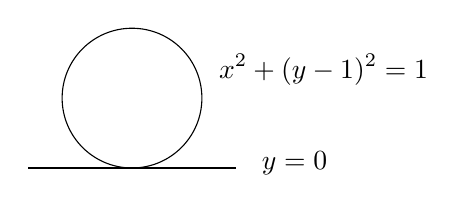
\begin{tikzpicture}[x=0.75pt,y=0.75pt,yscale=-1,xscale=1]
			%uncomment if require: \path (0,300); %set diagram left start at 0, and has height of 300
			
			%Straight Lines [id:da9022525264933119] 
			\draw    (44,106) -- (144,106) ;
			%Shape: Circle [id:dp5620106547865036] 
			\draw   (60.33,72.33) .. controls (60.33,53.74) and (75.41,38.67) .. (94,38.67) .. controls (112.59,38.67) and (127.67,53.74) .. (127.67,72.33) .. controls (127.67,90.93) and (112.59,106) .. (94,106) .. controls (75.41,106) and (60.33,90.93) .. (60.33,72.33) -- cycle ;
			
			% Text Node
			\draw (155.33,97) node [anchor=north west][inner sep=0.75pt]   [align=left] {$\displaystyle y=0$};
			% Text Node
			\draw (134.67,50) node [anchor=north west][inner sep=0.75pt]   [align=left] {$\displaystyle x^{2} +( y-1)^{2} =1$};
		\end{tikzpicture}
	\end{center}
	
	直观上, 直线与圆相切, 两者在相切处有一条公共的 ``无穷小线段''. 更一般地, 任意两条相切的曲线都有一条公共的形如 $D$ 的无穷小线段, 这便是两条曲线共同的切向量.
\end{example}

\paragraph{Kock--Lawvere 公理与导数}

~

\begin{axiom}
	[label={Kock--Lawvere-D}]
	{(Kock--Lawvere 公理)}
	对任意映射 $f \colon D \to R$, 存在唯一的 $a,b\in R$,
	使得
	$$
	f(d) = a + d\cdot b,\quad\forall d\in D.
	$$
	换言之, 作为 $R$-代数有
	$$
	\operatorname{Hom}(D,R) \simeq R[x]/(x^2).
	$$
\end{axiom}

Kock--Lawvere 公理反映了如下的直观: $R$ 上的一个函数在一个很小的邻域上近乎是一次函数.
由此, 我们立刻得到如下的推论.

\begin{propdef}
	{(导函数)}
	对任意函数 $f\colon R\to R$, 存在唯一的函数 $f' \colon R \to R$ 满足
	$$
	f(x+d) = f(x) + d \cdot f'(x),\quad \forall x\in R\,\forall d\in D.
	$$
	称 $f'$ 为 $f$ 的\emph{导函数}. 归纳地定义 $k$ 阶导数 $f^{(k)}(x)$.
\end{propdef}

也就是说, 综合微分几何要求任何函数 $R\to R$ 都是任意次可导的.

\paragraph{Weil 代数与无穷小几何对象}

~

无穷小线段 $D$ 对应代数 $R[x]/(x^2)$. 一般地, 在代数--几何对偶中与无穷小几何对象相对应的代数是 $R$ 上的 \emph{Weil 代数}\footnote{Weil 代数有两种含义, 这里所说的不是来自 Lie 代数的那种 Weil 代数.}.
\begin{definition}
	[label={SDG-Weil-algebra}]
	{(Weil 代数)}
	Weil 代数是形如 $W = R \oplus J$ 的 $R$-代数,
	其中 $J$ 是有限生成自由 $R$-模,
	且为幂零理想. 等价地,
	$$
	W = R[x_1,\cdots,x_n]/I,
	$$
	且存在正整数 $N$ 使得 $x_i^N \in I\,(i=1,\cdots,n)$.
\end{definition}

\begin{remark}
	{}
	上面的概念在 ``经典数学'' (经典逻辑) 中对应\emph{局部 Artin 代数}, 其中 Artin 代数是指不存在无限的理想下降链 (这称为\emph{下降链条件}) 的代数.
	设 $k$ 为域, $A$ 是局部 Artin $k$-代数, $\mathfrak m$ 是 $A$ 的唯一极大理想, 并且额外假设 $k \to A/\mathfrak m$ 是同构.%其剩余域 (residue field).
	可以证明\footnotemark $A \simeq k\oplus\mathfrak m$, $\mathfrak m$ 是有限维 $k$-线性空间且为幂零理想. 定义 \ref{SDG-Weil-algebra} 即是这个结果的类比.
	
	局部 Artin 环在代数几何的形变理论中有重要作用, 这正是因为它对应无穷小几何对象.
\end{remark}

\footnotetext{由中山 (Nakayama) 引理以及下降链条件可得 $\mathfrak m$ 幂零; 又由下降链条件可得每个 $\mathfrak m^j / \mathfrak m^{j+1}$ 是有限维 $k$-线性空间, 从而 $A$ 是有限维 $k$-线性空间.}

\begin{definition}
	{(Weil 代数的谱)}
	对于 Weil 代数 $W$, 定义 $W$ 的\emph{谱}为 $R$-代数同态的空间
	$$
	\operatorname{Spec}W = \operatorname{Hom}_{R\mathsf {Alg}}(W,R),
	$$
	称之为\emph{无穷小几何对象}.
\end{definition}

\begin{example}
	{(常见的无穷小几何对象)}
	\begin{itemize}
		\item 点 $$\text{pt} \simeq \{x\in R\mid x=0\} = \operatorname{Spec} R;$$
		\item 无穷小线段的平方 $$D^2 \simeq \{(x,y)\in R^2 \mid x^2=y^2=0\} = \operatorname{Spec}R[x,y]/(x^2,y^2);$$
		\item $R^2$ 上原点的一阶无穷小邻域 $$D(2) := \{(x,y)\in R^2\mid x^2=xy=y^2=0\} = \operatorname{Spec}R[x,y]/(x^2,xy,y^2);$$
		\item 高阶无穷小邻域
		$$
		D_k := \{x\in R\mid x^{k+1}=0\} = \operatorname{Spec}R[x]/(x^{k+1})\, (k=1,2,3,\cdots).
		$$
	\end{itemize}
\end{example}

前面介绍的 Kock--Lawvere 公理可表述为 $\operatorname{Hom}(\operatorname{Spec}R[x]/(x^2),R) \simeq R[x]/(x^2)$. 类似地有如下公理.

\begin{axiom}
	{(Kock--Lawvere 公理)}
	对于 Weil 代数 $W$, 有
	$$
	\operatorname{Hom}(\operatorname{Spec}W,R)\simeq W.
	$$
\end{axiom}

\begin{remark}
	{(Weil 代数与 Kock--Lawvere 公理的直观)}
	设 $W=R\oplus J$ 是 Weil 代数. 投影 $W \to R$ 对应点 $\text{pt}$ 到无穷小几何对象 $\operatorname{Spec}W$ 的\emph{原点}的嵌入 $$\text{pt} = \operatorname{Spec} R \to \operatorname{Spec}W.$$
	Kock--Lawvere 公理说的是 Weil 代数 $W$ 等同于 $\operatorname{Spec}W$ 上的函数代数. 投影 $W\to R$ 可视为 $\operatorname{Spec}W$ 上的函数在原点处取值; 理想 $J$ 是投影 $W\to R$ 的核, 可视为在原点取值为 $0$ 的函数的集合.
	要求 $J$ 为\emph{幂零}理想, 也即要求在原点取值为 $0$ 的函数都幂零, 直观上说明 $\operatorname{Spec}W$ 是 ``无穷小'' 的.
\end{remark}

Lawvere 以如下的性质刻画无穷小几何对象.

\begin{definition}
	{(无穷小对象, 奇妙右伴随)}
	对于空间 $S$, 若 $(-)^S$ 有右伴随, 则称 $S$ 为\emph{无穷小对象}. 记该右伴随为 $(-)_S$, 称之为\emph{奇妙右伴随} (amazing right adjoint).
\end{definition}

\begin{example}
	{}
	在集合范畴 $\mathsf {Set}$ 中, 只有终对象 $1$ 是无穷小对象.
\end{example}

\begin{remark}
	[label={infinitesimal-object-intuition}]
	{}
	回忆对\topos{}中任意对象 $S$, $(-)^S$ 都有左伴随 $(-)\times S$, 而 $(-)^S$ 有右伴随是非常稀奇的事情. 重要的是此时 $(-)^S$ \emph{保持余极限}. 一个直观如下. 设空间 $X$ 被一族空间 $U_i$ 覆盖 ($X$ 可写成 $U_i$ 和 $U_i\times_X U_j$ 的某种余极限), 那么 $X^S$ 也被 $U_i^S$ 覆盖, 即 $S$ 到 $X$ 的任何映射都必须穿过某个 $U_i$; 这是 $S$ 的像 ``太小'' 导致的.
	
	类似的性质在不是\topos{}的范畴中也有用处. 例如 Abel 群范畴 $\mathsf {Ab}$ 中, 函子 $\operatorname{Hom}(A,{-})$ 保持余极限当且仅当 $A$ 是有限生成投射 $\mathbb{Z}$-模, 这也是一种 ``小'' 的性质.
	
	%映射 $X^D \to Y$ 等同于映射 $X \to Y_D$
\end{remark}

\todo{使用 SDG 的例子, 如 Riemann 曲率}

\todo{无穷小对象的定义, amazing right adjoint}

\subsection{综合微分几何的模型}

本小节介绍综合微分几何的一些模型. 相对简单的模型就能实现 Kock--Lawvere 公理; 而为了使模型满足更多的公理, 以及更加贴近传统的微分几何 (更加 ``有用''), 我们就需要作越来越复杂的调整.
构造综合微分几何模型的贯穿始终的思想是\emph{代数--几何对偶}.

\subsubsection{``代数'' 模型}

首先考虑一个最简单的模型.
\begin{definition}
	[label={SDG-algebraic-model}]
	{}
	考虑有限表现仿射 $\mathbb{R}$-概形范畴 $\mathbb{R}\mathsf{Alg}_{\text{fp}}^\op$.
	回忆, 有限表现 $\mathbb{R}$-代数即形如 $\mathbb{R}[x_1,\cdots,x_n]/(f_1,\cdots,f_m)$ 的代数; 对于有限表现 $\mathbb{R}$-代数 $A$, 以 $\operatorname{Spec} A$ 表示其在对偶范畴中的化身.
	
	所谓\emph{代数模型} (algebraic model) 是 $\mathbb{R}\mathsf{Alg}_{\text{fp}}^\op$ 上的层\topos{} $$\mathsf {Fun}(\mathbb{R}\mathsf{Alg}_{\text{fp}},\mathsf {Set}).$$
\end{definition}

\begin{definition}
	{(直线)}
	定义 \emph{直线}
	$$
		R
		:=\yo(\operatorname{Spec}\mathbb{R}[x]).
	$$
\end{definition}

\begin{remark}
	{}
	这里考虑的\topos{}是 $\mathbb{R}$-代数的\emph{分类\topos{}}, 而 $R$ 是其中的\emph{一般 $\mathbb{R}$-代数} (generic $\mathbb{R}$-algebra).
	
	这些结论对有限生成 $\mathbb{R}$-代数范畴同样成立.
\end{remark}

注意到对 $A\in\mathbb{R}\mathsf {Alg}_{\text{fp}}$,
$$
R(A)=\operatorname{Hom}_{\mathbb{R}\mathsf{Alg}_{\text{fp}}^\op}(\operatorname{Spec}A,\operatorname{Spec}\mathbb{R}[x]) = \operatorname{Hom}_{\mathbb{R}\mathsf {Alg}_{\text{fp}}}(\mathbb{R}[x],A) \simeq A\text{ (作为集合)},
$$
我们发现, $R$ 正是代数范畴到集合范畴的遗忘函子
$$
R\simeq \text{遗忘}
\colon \mathbb{R}\mathsf{Alg}_{\text{fp}} \to \mathsf {Set}.
$$
因此, 使用米田方法, 我们就得到
\begin{prop}
	{}
	$R$ 是交换环.
\end{prop}

有了 $R$, 我们考虑 ``由方程定义的子流形''
$$
M = \{(x_1,\cdots,x_n)\in R^n\mid f_1=\cdots=f_m=0\},
$$
其中 $f_1,\cdots,f_m\in \mathbb{R}[x_1,\cdots,x_n]$ 是多项式. 其范畴语义为拉回
% https://q.uiver.app/#q=WzAsNCxbMSwxLCJSXm0iXSxbMCwxLCJSXm4iXSxbMSwwLCIwIl0sWzAsMCwiTSJdLFsxLDAsIihmXzEsXFxjZG90cyxmX20pIiwyXSxbMywxXSxbMywyXSxbMiwwXV0=
\[\begin{tikzcd}[ampersand replacement=\&]
	M \& 0 \\
	{R^n} \& {R^m,}
	\arrow["{(f_1,\cdots,f_m)}"', from=2-1, to=2-2]
	\arrow[from=1-1, to=2-1]
	\arrow[from=1-1, to=1-2]
	\arrow[from=1-2, to=2-2]
\end{tikzcd}\]
对应 $\mathbb{R}\mathsf {Alg}$ 中的推出
% https://q.uiver.app/#q=WzAsNCxbMSwxLCJcXG1hdGhiYntSfVt5XzEsXFxjZG90cyx5X21dIl0sWzAsMSwiXFxtYXRoYmJ7Un1beF8xLFxcY2RvdHMseF9uXSJdLFsxLDAsIlxcbWF0aGJie1J9Il0sWzAsMCwiTSJdLFswLDEsIihmXzEsXFxjZG90cyxmX20pIl0sWzEsM10sWzIsM10sWzAsMl1d
\[\begin{tikzcd}[ampersand replacement=\&]
	? \& {\mathbb{R}} \\
	{\mathbb{R}[x_1,\cdots,x_n]} \& {\mathbb{R}[y_1,\cdots,y_m],}
	\arrow["{y_i\mapsto f_i}", from=2-2, to=2-1]
	\arrow[from=2-1, to=1-1]
	\arrow[from=1-2, to=1-1]
	\arrow[from=2-2, to=1-2]
\end{tikzcd}\]
故
$$
M = \yo(\operatorname{Spec}\mathbb{R}[x_1,\cdots,x_n]/(f_1,\cdots,f_m)).
$$

\begin{definition}
	{(直线上原点的一阶无穷小邻域)}
	定义
	$$
	D := \{x\in R\mid x^2=0\} =  \yo\big({\operatorname{Spec}\mathbb{R}[x]/(x^2)}\big).
	$$
\end{definition}

我们验证它满足公理 \ref{Kock--Lawvere-D}, 以外部语言叙述即
\begin{prop}
	{}
	$$
	R^D(A) \simeq  A[x]/(x^2).
	$$
\end{prop}

\begin{proof}
	由预层\topos{}指数对象的构造 (命题 \ref{presheaf-category-exponential} 的证明),
	\begin{align*}
		R^D(A) &= \operatorname{Hom}(\yo(\operatorname{Spec}A)\times D,R)\\
		&\simeq \operatorname{Hom}\big(\yo(\operatorname{Spec}A)\times\yo(\operatorname{Spec}\mathbb{R}[x]/(x^2)),
		\yo(\operatorname{Spec}\mathbb{R}[x])\big)\\
		&\simeq \operatorname{Hom}\big(\yo(\operatorname{Spec}A\times\operatorname{Spec}\mathbb{R}[x]/(x^2)),
		\yo(\operatorname{Spec}\mathbb{R}[x])\big)\\
		&\simeq\operatorname{Hom}_{\mathbb{R}\mathsf{Alg}}(\mathbb{R}[x],A\otimes \mathbb{R}[x]/(x^2))\\
		&\simeq A\otimes \mathbb{R}[x]/(x^2))\simeq A[x]/(x^2) \text{ (作为集合).}
	\end{align*}
	其中用到 $\mathbb{R}$-代数的张量积是 $\mathbb{R}\mathsf{Alg}$ 中的和, 即 $\mathbb{R}\mathsf{Alg}^\op$ 中的积.%; 而 $\yo(A)\times\yo(B) \simeq \yo(A\times B)$.
\end{proof}





\subsubsection{光滑代数}

$\mathbb{R}$-代数上的运算是多项式运算; 若将多项式运算扩充为全体 ``光滑'' 运算, 则可产生一个更接近微分几何的模型.

\begin{definition}
	{(光滑代数)}
	\emph{光滑代数} ($C^\infty$-代数) 是指满足如下条件的集合 $A$: 对每个非负整数 $n$ 与每个 $n$ 元光滑函数 $f\in C^\infty (\mathbb{R}^n,\mathbb{R})$ 都有一个 $n$ 元运算, 称为\emph{光滑运算} $A(f)\colon A^n\to A$,
	使得 $f\mapsto A(f)$ 保持复合, 即对于 $h = g \circ (f_1,\cdots,f_k)$, 有
	$$A(h) = A(g) \circ (A(f_1),\cdots,A(f_k)).$$ 换言之, 光滑代数是 Lawvere 理论 $\mathsf {CartSp}$ 的模型 (例 \ref{Lawvere-theory-CartSp}). 光滑代数的同态是保持所有光滑运算的映射. 记光滑代数的范畴为 $C^\infty\mathsf{Alg}$.
\end{definition}

\begin{remark}
	[label={remark-smooth-algebra-R-algebra}]
	{}
	如上定义的 $C^\infty$-代数首先是 $\mathbb{R}$-代数: 考虑 $0$ 元函数 $\mathbb{R}^0\to \mathbb{R}$ 就得到了常量 $A^0\to A$,
	考虑加法与乘法函数 $+,\times\colon \mathbb{R}^2\to \mathbb{R}$ 就得到 $A$ 上的加法与乘法, 考虑映射 $\mathbb{R}^3\to \mathbb{R}, (x,y,z)\mapsto x(y+z) = xy+xz$, 使用 $f\mapsto A(f)$ 保持复合的条件, 就得到 $A$ 上的分配律, 如此这般.
\end{remark}

\begin{example}
	{}
	设 $M$ 是光滑流形, 那么 $M$ 上的光滑函数空间 $C^\infty (M)$ 构成光滑代数: 对 $f\in C^\infty (\mathbb{R}^n,\mathbb{R})$, 定义 $A(f)(f_1,\cdots,f_n)=f\circ (f_1,\cdots,f_n)$.
\end{example}

\begin{example}
	{}
	$\mathbb{R}[\varepsilon]/(\varepsilon^2)$ 是光滑代数: 对 $f\in C^\infty (\mathbb{R}^n,\mathbb{R})$, 定义 $$
	A(f)(a_1+b_1 \varepsilon,\cdots,a_n+b_n \varepsilon)
	=f(a_1,\cdots,a_n)
	+\sum_i \frac{\partial f}{\partial x_i}\Big|_{(a_1,\cdots,a_n)} b_i \varepsilon.$$
	$\mathbb{R}[\varepsilon]/(\varepsilon^2)$ 可视为 ``无穷小线段上的光滑函数空间''.
\end{example}

\begin{example}
	{}
	光滑流形上一点处的光滑函数芽 (定义 \ref{germ-and-stalk}) 构成光滑代数.
\end{example}

%\todo{使用一般 Lawvere 代数中有限生成的概念}
%我们需要有限生成 $C^\infty$-代数的概念.
类比于 $\mathbb{R}[x_1,\cdots,x_n]$ 是 $n$ 个元素生成的自由 $\mathbb{R}$-代数 (交换含幺代数), 有如下命题.

\begin{prop}
	[label={freely-generated-smooth-algebra}]
	{}
	$C^\infty (\mathbb{R}^n)$ 是 $n$ 个元素生成的\emph{自由光滑代数}.
\end{prop}

\begin{proof}
	要证明的是对任意光滑代数 $A$ 与任意 $n$ 个元素 $a_1,\cdots,a_n \in A$,
	存在唯一的同态 $\varphi\colon C^\infty (\mathbb{R}^n) \to A$ 将每个坐标函数 $x_i$ 映射到 $a_i$.
	由定义, 对任意 $f\in C^\infty (\mathbb{R}^n)$,
	$\varphi$ 必须把 $f = f\circ (x_1,\cdots,x_n)$ 映射到 $f(a_1,\cdots,a_n)$, 这便唯一确定了 $\varphi$; 而它确实将投影 $x_i$ 映射到 $a_i$: $x_i(a_1,\cdots,a_n) = a_i$.
\end{proof}

\newcommand{\locus}{处所}

%\todo{有限表现 vs 有限生成}

类比于\fm{}与位象的关系, 以及环与仿射概形的关系, 我们作如下的定义. 其中记号遵循 Moerdijk 与 Reyes \cite{MSIA}.

\begin{definition}
	{(光滑\locus{})}
	定义\emph{光滑\locus{}} (smooth locus, 复数 loci) 的范畴 $\mathbb L$ 为有限生成光滑代数范畴的对偶,
	$$
	\mathbb L:= C^\infty \mathsf {Alg}_{\text{fg}}^{\op},
	$$
	对于光滑代数 $A$,
	记 $\ell A$ 为 $A$ 在对偶范畴中的化身.
\end{definition}

我们发现\topos{} $\widehat {\mathbb L} = \mathsf {Fun}(C^\infty \mathsf {Alg}_{\text{fg}},\mathsf {Set})$ 是综合微分几何某种意义上的模型 (不过它尚且缺少一些微分几何关心的性质).

\begin{definition}
	{}
	定义\emph{直线}
	$$
	R := \yo(\ell C^\infty(\mathbb{R})).
	$$
\end{definition}


\section{量子理论与 Bohr 意象}

\philoquote{A description of physical reality is made in terms of two sets of objects: observables and states.}{Ludwig Faddeev, \emph{Elementary Introduction to Quantum Field Theory }}

对于经典力学与量子力学系统, 最核心的对象是其中的\emph{状态}与\emph{可观测量}.
量子理论有多种不同的公理化. 粗略地说, 我们考虑的一个量子系统由一个 $C^*$-代数 $\mathcal A$ 表示, 可观测量是这个 $C^*$-代数中的自伴元素, 而系统的状态是这个代数到 $\mathbb{C}$ 的某种映射 $$\rho\colon \mathcal A \to \mathbb{C}.$$ 人们常常以一个 Hilbert 空间 $H$ 表示系统中的纯态 (pure states), 而可观测量则被表示为 $H$ 上的自伴算子, 即有表示 $$\pi\colon \mathcal A \to \operatorname{End}(H).$$ 纯态 $\psi\in H$ 对应的映射则是
$$
\rho\colon A\mapsto \langle\psi | A | \psi \rangle := \langle\psi,\pi(A)\psi\rangle,
$$
它给出状态 $\psi$ 下可观测量 $A$ 的 ``期望值''.

\subsection{$C^*$-代数, 经典语境与 Bohr 景}

\begin{definition}
    {($C^*$-代数)}
    \emph{$C^*$-代数}是 $\mathbb{C}$ 上的 Banach 代数 $\big(\mathcal A,\|{-}\|\big)$,
    带有 ``伴随'' 运算 $(-)^*\colon \mathcal A \to \mathcal A$,
    满足对任意 $x\in \mathcal A$,
    \begin{multicols}
    	{2}
    	\begin{itemize}
    		\item $(a^*)^*=a$,
    		\item $(ab)^*=b^*a^*$,
    		\item $(\lambda a)^*=\bar\lambda a^*\,(\lambda\in\mathbb{C})$,
    		\item $\|a^* a\|=\|a\|\|a^*\|=\|a\|^2$.
    	\end{itemize}
    \end{multicols}
    $C^*$-代数的 $*$-子代数是指关于 $(-)^*$ 封闭的子代数.
\end{definition}

\begin{example}
    {}
    对于 Hilbert 空间 $H$, $H$ 上的有界线性算子的代数 $\mathcal B(H)$ 是 $C^*$-代数, 其中 $a^*$ 是 $a$ 的伴随算子. 事实上, 每个 $C^*$-代数都同构于某个形如 $\mathcal B(H)$ 的代数的 $*$-子代数, 因此后者也可作为 $C^*$-代数的一种具体定义.
\end{example}

\begin{definition}
	{(量子力学系统, 可观测量)}
	\begin{itemize}
		\item 一个\emph{量子力学系统} (quantum mechanical system) 是一个 $C^*$-代数 $\mathcal A$;
		\item 系统中的\emph{可观测量} (observable) 是 $\mathcal A$ 中的自伴元素, 即满足 $a^*=a$ 的元素;
		\item 系统中的\emph{状态} (state) 是线性函数 $\rho\colon \mathcal A\to \mathbb{C}$, 满足
		\begin{itemize}
			\item (正性) $\rho(aa^*)\geq 0$;
			\item (归一性) $\rho(1)=1$.
		\end{itemize}
	\end{itemize}
\end{definition}

我们给出经典力学系统的一种定义. 注意经典与量子系统的相似性.

\begin{definition}
	{(Poisson 代数)}
	\emph{Poisson 代数}是 $\mathbb{R}$ 上的含幺交换结合代数 $\mathcal A$ 配备一个运算 $\{-,-\}\colon \mathcal A\otimes \mathcal A\to \mathcal A$, 称为 \emph{Poisson 括号}, 满足
	\begin{itemize}
		\item $(\mathcal A,\{-,-\})$ 是 Lie 代数;
		\item 对任意 $a\in A$, $\{a,-\}\colon A\to A$ 是导子, 也即 $\{a,xy\}=\{a,x\}y+x\{a,y\}$.
	\end{itemize}
\end{definition}

\begin{example}
	{}
	熟悉经典力学的读者知道, 辛流形 $(X,\omega)$ 上的光滑函数代数 $C^\infty (X)$ 有自然的 Poisson 代数结构: 对 $f\in C^\infty (X)$ 定义向量场 $v_f$ 满足 $\omega(v_f,-) = df$, 则 $\{f,g\}:=\omega(v_f,v_g)$ 给出 $C^\infty (X)$ 上的 Poisson 代数结构.
\end{example}

\begin{definition}
	[label={classical-mechanical-system}]
	{(经典力学系统)}
	\begin{itemize}
		\item 一个\emph{经典力学系统} (classical mechanical system) 是一个 Poisson 代数 $(\mathcal A,\{-,-\})$;
		\item 系统中的\emph{可观测量} (observable) 是 $\mathcal A$ 中的元素;
		\item 系统中的\emph{状态} (state) 是线性函数 $\rho\colon \mathcal A\to \mathbb{R}$, 满足
		\begin{itemize}
			\item (正性) $\rho(a^2)\geq 0$;
			\item (归一性) $\rho(1)=1$.
		\end{itemize}
		\item 系统中的\emph{纯态} (pure state) 是满足上面条件的\emph{代数同态} $\mathcal A\to\mathbb{R}$.
	\end{itemize}
\end{definition}

\begin{example}
	{}
	由定义 \ref{classical-mechanical-system}, 对于辛流形 $(X,\omega)$, $X$ 上的一个点 $p$ 对应一个纯态 $C^\infty (X)\to\mathbb{R},f\mapsto f(p)$.
\end{example}

Heisenberg 不确定性原理表明, 不交换的可观测量不可同时确定, 而一族相交换的可观测量可以同时确定. 因此我们格外关注那些交换的子代数.

\begin{definition}
    {(经典语境)}
    对于量子力学系统 $\mathcal A$, 称 $\mathcal A$ 的一个交换 $*$-子代数为一个\emph{经典语境} (classical context).
    记 $\mathcal C(\mathcal A)$ 为 $\mathcal A$ 的交换 $*$-子代数在包含关系下构成的偏序集.
\end{definition}

\begin{remark}
    {}
    语境这个名字的含义是, 一个可观测量只在某些特定的语境 (也就是包含它的那些语境) 下才有确定的值. 在一个固定的语境中, 可观测量的表现无异于一个经典系统.
\end{remark}

这里我们稍微偏题, 介绍偏序集上的层.

\todo{移到层论那一章}

\begin{definition}
    {(Alexandorff 空间)}
    若一个拓扑空间中开集的任意交仍是开集, 则称其为 \emph{Alexandorff 空间}.
\end{definition}

\begin{definition}
    {(Alexandroff 拓扑)}
    设 $P$ 为偏序集. 定义 $P$ 上的 \emph{Alexandroff 拓扑}是以向上封闭集为开集的拓扑. 其中, 称 $Q\subset P$ 为\emph{向上封闭集}是指对任意 $x\in Q,y\in P$, 若 $x\leq y$, 则 $y\in Q$. 这给出了函子
    \[
    \operatorname{Alex}\colon \mathsf {Poset} \to \mathsf {Top}.
    \]
\end{definition}

\begin{prop}
    {}
    对任意偏序集 $P$, $P$ 上的预层可自然延拓为 $P$ 的 Alexandroff 拓扑上的层.
\end{prop}

% sheaf vs cosheaf
%
%\begin{definition}
%    {(Bohr 景)}
%    范畴, 也称 \emph{Bohr 景}. Bohr 景上的意象将是我们主要的研究对象.
%\end{definition}

\subsection{Bohr 意象}

\begin{definition}
    {(Bohr 意象)}
    称 $\mathcal C(\mathcal A)$ 上的预层意象为 \emph{Bohr 意象}.
\end{definition}

一个量子系统的\emph{状态} (state) 是一个线性映射 $A \to \mathbb{C}$

\begin{definition}
    {(Gelfand 谱)}
    对于交换 $C^*$-代数 $A$, 定义其 \emph{Gelfand 谱}
$$
\Sigma(A) := \{C^*\text{-代数同态}\,\lambda\colon A \to\mathbb{C}\},
$$
其拓扑为使得所有映射 $\Sigma(A)\to\mathbb{C}, \lambda \mapsto \lambda (x)$ 都连续的最弱拓扑. 由 Gelfand--Mazur 定理, Gelfand 谱 $\Sigma(A)$ 也是 $A$ 的极大理想的集合.
\end{definition}

$\Sigma(A)$ 上拓扑的定义旨在保证每个元素 $x\in A$ 都对应 $\Sigma(A)$ 上的一个复值连续函数. 如下定理表明这个对应实际上是一个同构; 这是代数--几何对偶的一例.

\begin{prop}
    {(Gelfand--Naimark 对偶)}
    记 $\mathsf {CC}^*$ 为交换 $C^*$-代数的范畴, $\mathsf{CHaus}$ 为紧 Hausdorff 空间的范畴,
    那么 Gelfand 谱给出反变函子 $\Sigma\colon \big(\mathsf {CC}^*\big)^{\op} \to \mathsf {CHaus}$, 且有范畴等价
    \[\begin{tikzcd}[ampersand replacement=\&]
    	{\big(\mathsf {CC}^*\big)^{\op}} \& {\mathsf {CHaus},}
    	\arrow["\Sigma", shift left, from=1-1, to=1-2]
    	\arrow["{C({-},\mathbb{C})}", shift left, from=1-2, to=1-1]
    \end{tikzcd}\]
    其中 $C(X,\mathbb{C})$ 是空间 $X$ 上复值连续函数的 $C^*$-代数.
\end{prop}

可观测量代数与状态空间互为对偶. 经典力学中, 可观测量是状态空间上的函数; 反过来, 状态空间上的点可视为可观测量代数到 $\mathbb{R}$ 的代数同态.
完全类似地, 在量子力学中, 给定语境 $A$, 对应的 "状态空间" $\Sigma(A)$ 中的点就是 $A$ 到 $\mathbb{C}$ 的代数同态, 而 $A$ 中的可观测量则可视为状态空间 $\Sigma(A)$ 上的函数.

\begin{definition}
    {(谱预层)}
    对于语境 $A_1 \subset A_2$, 有限制映射 $\Sigma(A_2)\to\Sigma(A_1)$. 这定义了 $\mathcal C(\mathcal A)$ 上的预层 $\Sigma$.
\end{definition}

\begin{remark}
    {}
    预层 $\Sigma$ 整合了所有经典语境的几何信息.
    
    一般而言, 一个可观测量只能给出预层 $\Sigma$ 的局部截面, 而无法给出整体截面.
\end{remark}

Bohr 意象中对象 $\Sigma$ 的构造可视为将 Gelfand 谱的构造由交换代数推广到非交换代数, 成为与交换子代数相对偶的空间的系统. 它实际上是 Bohr 意象中的内蕴位象 (internal locale). 而交换子代数的全体构成 Bohr 意象中的一个\emph{内蕴代数}. 由此, Bohr 意象的内语言允许我们像谈论经典态一样谈论量子态.

\subsection{Bohr 意象中的命题}



在一个经典系统中, 命题是状态空间的子集, 表示这个命题在何种状态下成立.
类似地, 量子系统中的命题是预层意象中 $\Sigma$ 的子对象, 或称子函子.

\section{Cohen 力迫法}

\label{Cohen-forcing}

1874 年, Georg Cantor 证明了自然数与实数 (又称连续统) 之间不存在一一对应\footnote{不过他的第一个证明并非现在流行的对角线论证.}. Cantor 接着于 1878 年提出了\emph{连续统假设} (continuum hypothesis),
$$
\fbox{在自然数集合 $N$ 与连续统 $PN$ 之间不存在其它的基数.}
$$

1940 年, Kurt G\"odel 证明连续统假设与 Zermelo--Fraenkel 集合论相容. 1963 年, Paul Cohen 证明了连续统假设独立于带有选择公理的 Zermelo--Fraenkel 集合论 (ZFC), 即 ZFC 既不能证明, 也不能证伪连续统假设.

% Boole 意象的内容放在了第一章末尾.

在 \ref{Boolean-topos} 节我们介绍了 Boole \topos{}. 我们可以在这样的\topos{}中做 ``经典数学''. 下面的内容本质上等同于 Cohen 证明连续统假设独立于 ZFC 所使用的方法, 只不过翻译到了\topos{}的语境.

\begin{prop}
	{}
	存在一个 Boole \topos{}, 其中选择公理成立, 而连续统假设不成立.
\end{prop}

\subsubsection{基础知识}

回忆任何\topos{}上都有一个 Lawvere--Tierney 拓扑 $\neg\neg$. 有趣的是, 它总是给出一个 Boole 意象.

\begin{prop}
	{}
	对任意\topos{} $\mathcal C$, $\operatorname{Sh}_{\neg\neg}\mathcal C$ 为 Boole \topos{}.
\end{prop}
\begin{proof}
	由 Boole \topos{}的内语言刻画 (\ref{internal-Boolean-topos}), 我们要在 $\operatorname{Sh}_{\neg\neg}\mathcal C$ 中证明 $\forall p\in\Omega (p\lor \neg p)$.
	% 需要几何态射在命题上的作用
	\todo{}
\end{proof}

\begin{definition}
	{(基数的比较)}
	对于一个\topos{}中的两个对象 $X,Y$, 若存在单射 $X\to Y$, 且 $\operatorname{Epi}(X,Y)\simeq 0$, 则称 $X$ 的基数小于 $Y$, 记为 $X<Y$.
\end{definition}

回忆 $\operatorname{Epi}(X,Y)$ 的定义 (\ref{set-of-epimorphisms}), $\operatorname{Epi}(X,Y)\simeq 0$ 当且仅当公式 $\forall f\in Y^X\,\neg(\operatorname{im}f = Y)$ 成立.



\section{凝聚态数学}

% 【潜水】岩豚鼠: 我们要解决拓扑abel群范畴不是abel范畴的问题, 首先要解决拓扑空间范畴中连续双射不可逆的问题. 注意到紧Hausdorff空间没有这个问题, 我们就尝试将一般的拓扑空间换成紧Hausdorff空间范畴上的层, 而这个景有一族基叫做投射有限集. 这里的拓扑是取连续满射为覆盖. 每个紧Hausdorff空间都被它自己的集合作为离散空间覆盖, 注意到紧Hausdorff空间到一般拓扑空间范畴的嵌入有个左伴随叫Stone—Cech紧化, 我们就可以把基取为离散空间的SC紧化.


% 第五章 分类\topos{}
\chapter{句法景与分类\topos{}}

\label{cla}

\minitoc

\section{句法范畴: 语法--语义对偶}

\todo{两种不同的 syntactic category}

%\todo{写成单独的一章?}

\philoquote{The importance of syntactic categories lies in the fact that they allow us to associate with a theory (in the sense of axiomatic presentation), which is a `linguistic',
	unstructured kind of entity, a well-structured mathematical object whose `geometry' embodies the syntactic aspects of the theory.}{Olivia Caramello, \cite{TST}}

%  A most notable fact is that the models of the theory can be recovered as functors defined on its syntactic category which respect the ‘logical’ structure on it.

逻辑学上有一个一般性的现象, 即理论 (一阶逻辑, 类型论等等) 与范畴之间的对应. 某些范畴可以为理论提供语义, 某些理论可以作为范畴的语法.
%
\todo{}

我们将看到语法--语义对偶也是一种代数--几何对偶\footnote{或许也可以反过来说代数--几何对偶不过是一种语法--语义对偶.}, 语法对应代数, 语义对应几何.

\subsection{类型论的语境范畴}

附录 \ref{appendix-type-theory} 节简单介绍了类型论.

\begin{definition}
	{}
	对于一种类型论 $T$, 其\emph{语境范畴} (category of contexts) $\operatorname{Con}(T)$ 定义如下.
	\begin{itemize}
		\item $\operatorname{Con}(T)$ 的\emph{对象}为类型论 $T$ 的\emph{语境};
		\item $\operatorname{Con}(T)$ 中的\emph{态射}为语境之间的\emph{代换}.
	\end{itemize}
\end{definition}



\subsection{一阶理论的句法范畴}

\begin{definition}
	[label={first-order-theory-syntactic-category}]
	{(一阶理论的句法范畴)}
	
	设 $\mathbb T$ 是符号表 $\Sigma$ 上的一阶理论. 定义\emph{句法范畴} (syntactic category) $\mathcal C_{\mathbb T}$, 其中
	\begin{itemize}
		\item \emph{对象}是 $\Sigma$ 上带有语境的公式 $(\vec x , \phi)$ 的 $\alpha$-等价类 ($\alpha$ 等价是指两个公式仅有变量名的差异);
		\item 对象 $(\vec x , \phi)$ 到 $(\vec y , \psi)$ 的\emph{态射} (其中不妨设语境 $\vec x , \vec y$ 不交) 是公式 $\theta(\vec x,\vec y)$ 的 $\mathbb T$-可证等价类, 满足 $\mathbb T$-可证的\emph{函数性}, 即如下相继式 $\mathbb T$-可证.
		\begin{itemize}
			\item $\phi\vdash_{\vec x} \exists \vec y \,\theta$, 含义是 ``对给定的 $\vec x$, 存在 $\vec y$ 满足 $\theta(\vec x,\vec y)$'';
			\item $\theta\vdash_{\vec x,\vec y} \phi \wedge \psi$,
			\item $\theta \wedge \theta[\vec z/\vec y] \vdash_{\vec x,\vec y,\vec z} \vec y = \vec z$, 这里 $\theta[\vec z / \vec y]$ 是指将 $\theta$ 中的 $\vec y$ 替换为 $\vec z$, 公式的含义是 ``对给定的 $\vec x$, 至多存在一个 $\vec y$ 满足 $\theta(\vec x,\vec y)$''.
		\end{itemize}
	\end{itemize}
\end{definition}

\begin{remark}
	{}
	句法范畴的态射又称\emph{变量代换}.
\end{remark}

\begin{remark}
	{}
	由定义, 一个理论的句法范畴依赖于理论所属的类别 (代数, 正则, 凝聚, $\cdots$). 一个代数理论也可以视为凝聚理论, 但一个代数理论的句法范畴与它作为凝聚理论的句法范畴不同.
\end{remark}

\subsection{代数理论的句法范畴--Lawvere 理论}

\todo{万有代数}

\begin{prop}
	{}
	对于代数理论 $\mathbb T$,
\end{prop}

\begin{example}
	[label={Lawvere-theory-CartSp}]
	{}
	$\mathsf {CartSp}$
\end{example}

\section{分类\topos{}}

\philoquote{
    The notion of classifying topos really formalizes the notion of ``content'' of a mathematical theory.
    If you discover that two theories have the same classifying topos, this means that the two theories tell the same story in different languages.
}{Olivia Caramello}

%分类\topos{}的角色类似于拓扑学中的分类空间:
有代数拓扑背景的读者知道, 对于拓扑群 $G$ 存在 ``分类空间'' $BG$,
使得 (足够好的) 空间 $X$ 上 $G$-主丛的等价类
一一对应于 $X$ 到 $BG$ 的映射同伦类 (被 $BG$ ``分类''),
$$
G\mathsf{-Bund} (X) \simeq [X,BG];
$$
从而恒等映射 $\operatorname{id}_{BG}$ 对应着 $BG$ 上一个 ``万有'' 的 $G$-主丛 $EG \to BG$,
``万有'' 意指任何 $G$-主丛都是通过某个映射 $X \to BG$ 将其拉回得到.
分类\topos{}不仅仅是分类空间的一个精神上的类比; 它某种意义上是分类空间的推广, 这种推广正是沿着 Grothendieck 的 ``\topos{}作为空间概念的推广'' 的思路.

类似地, 在许多情形下, \topos{}上的一种结构 $T$ 可由它到一个特殊的\topos{}的态射来分类, 这就是\emph{分类\topos{}}的概念;
某种结构 $T$ 的分类\topos{}应当视为 ``所有 $T$ 构成的空间'', 术语叫做\emph{模空间}.
若将\topos{} $\mathsf C$ 视为空间, 那么 $\mathsf C$ 上的一个结构 $T$ 可视为空间的 ``每一点'' 上都有一个结构 $T$,
从而这给出 $\mathsf C$ 到模空间的一个几何态射.
例如, 设 $\mathsf E$ 为环的分类\topos{}, 那么 $\mathsf E$ 应当视为 ``所有环构成的空间'' (上的层范畴), 拓扑空间 $X$ 上的一个环层即是 $X$ 的 ``每一点'' 上都有一个环,
这等同于 $\text{Sh}(X)$ 到 $\mathsf E$ 的一个几何态射.

分类\topos{}到自身的恒等态射对应着其上的 ``万有'' 的 $T$ 结构, 又称\emph{重言} (tautological) $T$ 结构.

\subsection{$G$-旋子的分类\topos{}}


下面的概念是 ``空间上的 $G$-主丛'' 的推广, 取自 \cite{SGL} VIII.2 节.
\begin{definition}
	[label={G-torsors-over-topos}]
	{(\topos{}上的 $G$-旋子)}
	设 $G$ 为离散群, 即 $\mathsf {Set}$ 中的群.
	设 $\gamma\colon \mathsf C\to \mathsf {Set}$ 是 $\mathsf {Set}$ 上的\topos{} (见命题 \ref{global-sections-geometric-morphism}). 定义 $\mathsf C$ 上的一个 $G$-\emph{旋子}\footnotemark (torsor) 为 $\mathsf C$ 的对象 $T$, 以及群对象 $\gamma^*(G)$ 在 $T$ 上的作用 $\mu\colon \gamma^*(G)\times T \to T$, 满足
	\begin{enumerate}[(i)]
		\item 映射 $T\to 1$ 为满射;
		\item 群作用 $\mu$ 诱导同构 $(\mu,\pi_2)\colon \gamma^*(G)\times T \to T\times T$.
	\end{enumerate}
\end{definition}
\footnotetext{Torsor 似乎没有通行的中文译名, 这可能是因为它在拓扑学中一般被称作\emph{主丛}. 这里我跟随我的一位老师译为\emph{旋子}.}

%\begin{remark}
%	{(条件 ii 的解读)}
%	群作用 $\mu$ 诱导同构 $(\mu,\pi_2)\colon \gamma^*(G)\times T \to T\times T$ 等价于 $\gamma^*(G)$ 在 $T$ 上的作用是自由且传递的.
%	
%\end{remark}

\begin{example}
	{(集合范畴中的 $G$-旋子)}
	由于集合范畴 $\mathsf {Set}$ 是一个点上的层范畴,
	$\mathsf {Set}$ 中的 $G$-旋子即是 ``一个点上的 $G$-主丛'',
	即一个非空集合 $T$, 带有 $G$-左作用 $\mu\colon G\times T \to T$, 满足 $(\mu,\pi_2)\colon G\times T \to T\times T$ 为双射.
	后一个条件等价于这个作用是自由且传递的:
	``自由'' 等价于 $(\mu,\pi_2)\colon G\times T \to T\times T$ 为单射, ``传递'' 等价于其为满射.
	
	有趣的是, 两个映射 $\mu,\pi_2\colon G\times T \to T$ 也可视为一个范畴 (具体地, $G$ 在 $T$ 上作用的\emph{作用群胚}) 的箭头集合到对象集合的两个映射, 分别将一个箭头映射到其终点与起点. 那么 $(\mu,\pi_2)\colon G\times T \to T\times T$ 为双射就是说, 作用群胚的任何两个对象 $x,y$ 之间有且仅有一个态射 $x\to y$.
\end{example}

\begin{example}
	{(空间上的 $G$-主丛)}
	仍设 $G$ 为离散群. 拓扑空间 $X$ 上的 $G$-主丛等价于 (或可定义为) 平展映射 $E \to X$, 带有 $X$ 上的 $G$-左作用 $G\times E \to E$, 使得每个纤维 $E_x$ 非空且带有 $G$ 的自由传递作用.
	
	可以证明, 这个定义等价于层\topos{} $\operatorname{Sh}(X)$ 上 $G$-旋子的定义.
\end{example}

\begin{example}
	{($G\mathsf {Set}$ 上的万有 $G$-旋子)}
	对于离散群 $G$, 考虑其自身作成的 $G$-右作用集合 $R_G$. 我们断言它是 $G\mathsf {Set}$ 上的 $G$-旋子.
	
	首先回忆几何态射 $\gamma\colon G\mathsf {Set} \to \mathsf {Set}$ (例 \ref{group-homomorphism-adjoint-triple-example-G-1}),
	其逆像函子 $\gamma^*\colon \mathsf {Set} \to G\mathsf {Set}$
	将集合对应到其自身, 带有平凡 $G$-右作用.
	群作用 $\mu\colon \gamma^*(G)\times R_G \to R_G$, $(g,h)\mapsto gh$ 是 $G$-集合的态射, 因为 $\mu(g,hk)=ghk=\mu(g,h)k$.
	映射 $(\mu,\pi_2)\colon \gamma^*(G)\times R_G\to R_G\times R_G$ 为 $(g,h)\mapsto (gh,h)$, 从而为 $G$-集合的同构.
	%\todo{写完万有 $G$-旋子}
\end{example}

\topos{}上的旋子是 ``旋子的理论'' 的模型.

\begin{definition}
	{($G$-旋子的理论)}
	设 $G$ 为离散群, 定义 $G$-旋子的理论 $\mathbb T_G$.
	其中只有一个类型 $T$, 对每个元素 $g\in G$ 都有一个一元函数符号 $g$, 公理如下.
	\begin{itemize}
		\item (\emph{群作用}) 对每一对 $g,h\in G$ 有一条公理 $\vdash_x g(hx)=(gh)x$ (注意这里没有用到任意量词 $\forall$);
		\item (\emph{非空}) $\vdash \exists x. \top$;
		\item (\emph{自由性}) 对每一对不同的 $g,h\in G$ 有一条公理 $(gx=hx)\vdash_x \bot$ (同上, 这里没有用到 $\forall$);
		\item (\emph{传递性}) $\displaystyle\vdash_{(x,y)}\bigvee_{g\in G}gx=y$.
	\end{itemize}
\end{definition}

理论 $\mathbb T_G$ 是一种几何理论 (定义 \ref{kinds-of-theories}), 因为它用到了 ``真'' $\top$, 存在量词 $\exists$, ``假'' $\bot$ 和无穷析取 $\bigvee$.

\subsection{子终对象的分类\topos}

考虑范畴 $\mathsf 2 = \{\bullet\longrightarrow\bullet\}$. 例 \ref{varying-set-topos} 介绍的 ``变集范畴'' $\mathsf {Fun}(\mathsf {2},\mathsf {Set})\simeq\widehat {\mathsf {2}}$ 还有一个特殊的名字叫 \emph{Sierpi\'nski \topos{}}, 因为它与 Sierpi\'nski 空间有关.

\begin{propdef}
	[label={Sierpinski-space}]
	{(Sierpi\'nski 空间)}
	开集函子 $\operatorname{Open}\colon \mathsf {Top}\to \mathsf {Set}$ 是可表函子, 其表示对象称为 \emph{Sierpi\'nski 空间}.
\end{propdef}

\todo{}

\subsection{群的分类\topos{}}

本节构造群的分类\topos{}. 群是一种 Lawvere 理论 (附录 \ref{universal-algebra} 节); 下面的论述适用于一般的 Lawvere 理论, 从而逐字逐句地替换可得到环, Boole 代数等结构的分类\topos{}.
%
% 回忆范畴中的群对象的概念. 设范畴 $\mathsf C$ 有有限积 (包括始对象 $1$), 那么 $\mathsf C$ 中的\emph{群}为对象 $G$, 带有元素 $e \colon 1 \to G$, 乘法 $\cdot \colon G\times G \to G$, 满足群的交换图.

%满足通常的交换环的图表, 例如分配律 $x(y+z)=xy+xz$ 对应交换图
%% https://q.uiver.app/#q=WzAsNCxbMCwwLCJSXFx0aW1lcyBSXFx0aW1lcyBSIl0sWzEsMCwiUlxcdGltZXMgUiJdLFsxLDEsIlIiXSxbMCwxLCJSXFx0aW1lcyBSIl0sWzAsMSwiKHgseSx6KVxcbWFwc3RvICh4LHkreikiXSxbMSwyLCJcXHRpbWVzIl0sWzAsMywiKHgseSx6KVxcbWFwc3RvICh4eSx4eikiLDJdLFszLDIsIisiLDJdXQ==
%\[\begin{tikzcd}[ampersand replacement=\&]
%	{R\times R\times R} \& {R\times R} \\
%	{R\times R} \& R.
%	\arrow["{(x,y+z)}", from=1-1, to=1-2]
%	\arrow["\times", from=1-2, to=2-2]
%	\arrow["{(xy,xz)}"', from=1-1, to=2-1]
%	\arrow["{+}"', from=2-1, to=2-2]
%\end{tikzcd}\]
%(这里使用了 \ref{Mitchell--Benabou-language} 节介绍的 Mitchell--B\'enabou 语言.)

设范畴 $\mathsf C$ 有有限积. $\mathsf C$ 中的群对象构成一个范畴 $\mathsf {Grp}(\mathsf C)$.
\ref{universal-algebra} 节提到它等同于群的 Lawvere 理论 $\mathbb T_{\text{Grp}}$ 到 $\mathsf C$ 的保持有限积的函子的范畴.
进一步, 对于两个具有有限积的范畴 $\mathsf C,\mathsf D$, 以及保持有限积的函子 $f \colon \mathsf C \to \mathsf D$, 有对应的函子
$\mathsf {Grp}(\mathsf C) \to \mathsf {Grp}(\mathsf D)$.% $\mathsf {Ring}(\mathsf C) \to \mathsf {Ring}(\mathsf D)$.

对于\topos{}间的几何态射 $f \colon \mathsf C \to \mathsf D$, 其逆像部分 (见定义 \ref{geometric-morphism}) $f^* \colon \mathsf D \to \mathsf C$ 保持有限极限, 故保持有限积, 从而诱导了函子 $\mathsf {Grp}(\mathsf D) \to \mathsf {Grp}(\mathsf C)$;
这表示 $\mathsf {Grp}(-)$ 关于\topos{}是 ``反变'' 的.

下面我们将构造一个\topos{} $\mathsf E$, 称为\emph{群的分类\topos{}}, 使得有自然的范畴等价
$$
\mathsf {Grp}(\mathsf C) \simeq \mathsf{Hom}(\mathsf C,\mathsf E).
$$

\subsection{环的分类\topos{}}

\todo{单独讲一下和代数几何的关系}

% 参考 Caramello 的 TST

%\paragraph{群}
%
%考虑范畴 $\mathsf A = (\mathsf {Grp}_{\text{f}})^\op$,
%
%\paragraph{环}
%
%考虑范畴 $\mathsf A = (\mathsf {Ring}_{\text{fp}})^\op$,
%其中 $\mathsf {Ring}_{\text{fp}}$ 是 ($\mathsf{Set}$ 中) \emph{有限表现} (finitely presented) 环的范畴 (见例 \ref{zariski-site}).
%$\mathsf A$ 中有一个特殊的对象 $A = \mathbb{Z}[x]$,
%也即仿射直线.

\subsection{几何理论的分类\topos{}}

\begin{definition}
    {(几何理论的句法景和分类\topos{})}
    设 $\mathbb T$ 为一几何理论.
    
    $\text{Sh}(\mathcal C_{\mathbb T},)$
\end{definition}

\todo{以 torsor 的句法景举例}

\appendix

% 附录 范畴论
\chapter{范畴论基础}

\section{伴随函子}

\subsection{伴随保持极限}

\begin{prop}
	[label={adjoints-preserve-limits}]
	{}
	右伴随保持极限, 左伴随保持余极限.
\end{prop}

\begin{proof}
	设有伴随
	% https://q.uiver.app/#q=WzAsMixbMCwwLCJcXG1hdGhzZiB7Q30iXSxbMSwwLCJcXG1hdGhzZiB7RH0iXSxbMSwwLCJGIiwyLHsib2Zmc2V0IjoyfV0sWzAsMSwiRyIsMix7Im9mZnNldCI6Mn1dLFsyLDMsIiIsMCx7ImxldmVsIjoxLCJzdHlsZSI6eyJuYW1lIjoiYWRqdW5jdGlvbiJ9fV1d
	\[\begin{tikzcd}[ampersand replacement=\&]
		{\mathsf {C}} \& {\mathsf {D},}
		\arrow[""{name=0, anchor=center, inner sep=0}, "F"', shift right=2, from=1-2, to=1-1]
		\arrow[""{name=1, anchor=center, inner sep=0}, "G"', shift right=2, from=1-1, to=1-2]
		\arrow["\dashv"{anchor=center, rotate=-90}, draw=none, from=0, to=1]
	\end{tikzcd}\]
	设 $X \colon I \to \mathsf C$ 是一个图 ($I$ 是小范畴).
	若极限 $\lim_i X_i$ 存在,
	则有自然同构
	\begin{align*}
		\operatorname{Hom}(-,G\lim_i X_i)
		&\simeq \operatorname{Hom}(F-,\lim_i X_i)\\
		&\simeq \lim_i \operatorname{Hom}(F-,X_i)\\
		&\simeq \lim_i \operatorname{Hom}(-,GX_i)\\
		&\simeq \operatorname{Hom}(-,\lim_i GX_i).
	\end{align*}
	由米田引理, 得同构 $G\lim_i X_i \simeq \lim_i GX_i$,
	故右伴随保持极限.
	另一结论由对偶性即证.
\end{proof}

\begin{example}
	{}
	遗忘函子 $\mathsf {Top} \to \mathsf {Set}$ 同时有左伴随和右伴随:
	% https://q.uiver.app/#q=WzAsMixbMCwwLCJcXG1hdGhzZiB7VG9wfSJdLFsyLDAsIlxcbWF0aHNmIHtTZXR9Il0sWzAsMSwiXFx0ZXh0e+mBl+W/mH0iLDAseyJsYWJlbF9wb3NpdGlvbiI6MjB9XSxbMSwwLCLnprvmlaMiLDIseyJsYWJlbF9wb3NpdGlvbiI6MjAsIm9mZnNldCI6NX1dLFsxLDAsIuW5s+WHoSIsMCx7ImxhYmVsX3Bvc2l0aW9uIjoyMCwib2Zmc2V0IjotNX1dLFszLDIsIiIsMSx7ImxldmVsIjoxLCJzdHlsZSI6eyJuYW1lIjoiYWRqdW5jdGlvbiJ9fV0sWzIsNCwiIiwxLHsibGV2ZWwiOjEsInN0eWxlIjp7Im5hbWUiOiJhZGp1bmN0aW9uIn19XV0=
	\[\begin{tikzcd}[ampersand replacement=\&]
		{\mathsf {Top}} \&\& {\mathsf {Set}}
		\arrow[""{name=0, anchor=center, inner sep=0}, "{\text{遗忘}}"{pos=0.2}, from=1-1, to=1-3]
		\arrow[""{name=1, anchor=center, inner sep=0}, "{\text{离散}}"'{pos=0.2}, shift right=5, from=1-3, to=1-1]
		\arrow[""{name=2, anchor=center, inner sep=0}, "{\text{平凡}}"{pos=0.2}, shift left=5, from=1-3, to=1-1]
		\arrow["\dashv"{anchor=center, rotate=-90}, draw=none, from=1, to=0]
		\arrow["\dashv"{anchor=center, rotate=-90}, draw=none, from=0, to=2]
	\end{tikzcd}\]
	因此这个遗忘同时保持极限与余极限; 换言之, 拓扑空间的极限与余极限可用底层集合的极限与余极限来计算.
\end{example}

\begin{prop}
	[label={adjoint-full-subcategory-equivalence}]
	{(伴随产生一对满子范畴的等价)}
	设有伴随
	% https://q.uiver.app/#q=WzAsMixbMCwwLCJcXG1hdGhzZiB7Q30iXSxbMSwwLCJcXG1hdGhzZiB7RH0iXSxbMSwwLCJGIiwyLHsib2Zmc2V0IjoyfV0sWzAsMSwiRyIsMix7Im9mZnNldCI6Mn1dLFsyLDMsIiIsMCx7ImxldmVsIjoxLCJzdHlsZSI6eyJuYW1lIjoiYWRqdW5jdGlvbiJ9fV1d
	\[\begin{tikzcd}[ampersand replacement=\&]
		{\mathsf {C}} \& {\mathsf {D},}
		\arrow[""{name=0, anchor=center, inner sep=0}, "F"', shift right=2, from=1-2, to=1-1]
		\arrow[""{name=1, anchor=center, inner sep=0}, "G"', shift right=2, from=1-1, to=1-2]
		\arrow["\dashv"{anchor=center, rotate=-90}, draw=none, from=0, to=1]
	\end{tikzcd}\]
	其单位和余单位分别为
	$\eta \colon \operatorname{id}_{\mathsf D} \to GF$,
	$\epsilon \colon FG \to \operatorname{id}_{\mathsf C}$.
	考虑
	\begin{itemize}
		\item $\mathsf C$ 中由使得 $\eta_X \colon X \to GF(X)$ 为同构的 $X$ 构成的满子范畴 $\widetilde {\mathsf C}$,
		以及
		\item $\mathsf D$ 中由使得 $\epsilon_Y \colon FG(Y)\to Y$ 为同构的 $Y$ 构成的满子范畴 $\widetilde {\mathsf D}$,
	\end{itemize}
	那么 $F$ 与 $G$ 限制为一对互逆的范畴等价
	$$
	\widetilde G\colon \widetilde {\mathsf C} \overset{\simeq}{\to} \widetilde {\mathsf D},\quad
	\widetilde F\colon \widetilde {\mathsf D} \overset{\simeq}{\to} \widetilde {\mathsf C}.
	$$
\end{prop}

\begin{proof}
	由条件, $\eta$ 限制为自然变换
	$$
	\widetilde \eta \colon
	\operatorname{id}_{\widetilde {\mathsf D}} \to \widetilde G \widetilde F,
	$$
	且 $\widetilde \eta$ 的每个分量 ${\widetilde \eta}_{X} \colon X \to \widetilde G \widetilde F (X)$ 均为同构.
	因此 $\widetilde \eta$ 为自然同构. 另一边类似.
\end{proof}
\section{预层范畴与米田引理}

固定如下记号: $\mathsf C$ 为小范畴, $\yo\colon \mathsf C \to \widehat {\mathsf C} = \mathsf {Fun}(\mathsf C^{\op},\mathsf {Set})$ 为米田嵌入. 本节参考了 \cite{SGL} I.5 节.

\label{yoneda}

\subsection{可表函子的余极限}

\begin{definition}
    [label={slice-over-presheaf}]
    {(元素的范畴)}
    对 $X\in\widehat {\mathsf C}$, 定义 $X$ 的\emph{元素的范畴} $\displaystyle\int_{\mathsf C}X$ 如下.
    其对象为 $(c,x)$, $x\in X(c)$,
    态射 $(c,x)\to (d,y)$ 为 $f\colon c\to d$, 满足 $f(x)=y$.
    
    %记 $X$ 的元素的范畴为
    由定义, 存在 ``投影'' 函子 $\pi_X\colon \displaystyle\int_{\mathsf C}X\to \mathsf C$, $(c,x)\mapsto c$.
\end{definition}

\begin{definition}
	{(元素的范畴, 等价定义)}
	由米田引理, $X$ 的元素的范畴等价于 (甚至同构于) 如下范畴: 其对象为态射 $\yo(c)\to X$, 其态射为形如
	$\begin{tikzcd}[ampersand replacement=\&,row sep=-1pt,column sep=small]
		{\yo(c)} \\
		\& X \\
		{\yo(d)}
		\arrow[from=1-1, to=2-2]
		\arrow[from=1-1, to=3-1]
		\arrow[from=3-1, to=2-2]
	\end{tikzcd}$ 的交换图.
\end{definition}

\begin{remark}
    {}
    若将 $X$ 视为 $\mathsf C$ 的 ``广义元素'', 则 $X$ 的元素的范畴可视为``俯范畴'' $\mathsf C /X$.
    
    此外, 也有人将这个范畴记作 $(\yo\downarrow X)$, 它还有一个令人迷惑的名称 ``逗号范畴'' (comma category).
\end{remark}

事实上, 所有态射 $\yo(c)\to X$ 共同将 $X$ 表示为一个余极限.

\begin{prop}
    {(预层为可表函子的余极限)}
    $\widehat {\mathsf C}$ 的对象 $X$ 是如下余极限:
    $$
    X \simeq \operatorname{colim}\Big(\begin{tikzcd}[ampersand replacement=\&]
    	{\displaystyle\int_{\mathsf C}X} \& {\mathsf C} \& {\widehat {\mathsf C}}
    	\arrow["\yo", from=1-2, to=1-3]
    	\arrow["{\pi_X}", from=1-1, to=1-2]
    \end{tikzcd}\Big).
    $$
    %函子 $\colon \displaystyle\int_{\mathsf C}X \overset{\pi}{\to} \widehat {\mathsf C}$ 的余极限.
\end{prop}

\begin{proof}
	任给余锥 $\big(\phi_{c,x}\colon \yo(c)\to Y\big)_{(c,x)}$,
	定义态射 $\eta\colon X\to Y$,
	$\eta_c\colon X(c)\to Y(c)$,
	$x\mapsto\phi_{c,x}$.
\end{proof}

\begin{example}
    {(单纯集)}
    对于 $\mathsf C= \Delta$ (例 \ref{Simplicial-Sets}),
    $\widehat {\mathsf C}$ 中对象 $X$ 的元素可视为单纯集 $X$ 中的单纯形, 包含退化的单纯形.
    此时上述命题即是说 $X$ 等同于其所有单纯形的粘合. 这符合了单纯集是由单纯形组成的直观.
\end{example}

\subsection{自由余完备化}

在上个小节, 我们看到 $\widehat {\mathsf C}$ 是 $\mathsf C$ 经过某种添加余极限的过程得到的余完备范畴. 称 $\widehat {\mathsf C}$ 为 $\mathsf C$ 的\emph{自由余完备化} (free cocompletion); 以下命题解释了这句话中 ``自由'' 的含义, 即余完备范畴到一般范畴的 ``遗忘'' 的左伴随.

\begin{prop}
	[label={free-cocompletion}]
    {}
    设 $\mathsf C$ 是(小)范畴, $\mathsf D$ 是余完备范畴,
    那么米田嵌入
    $\yo \colon \mathsf C \to \widehat {\mathsf C}$
    给出了等价
    $$
    \yo^*\colon \mathsf {Fun}^{\text{colim}}(\widehat {\mathsf C},\mathsf D) \overset{\simeq}{\longrightarrow} \mathsf {Fun}(\mathsf C,\mathsf D),
    $$
    其中 $\mathsf {Fun}^{\text{colim}}$ 表示\emph{保持余极限的}函子构成的范畴. 换言之, 对任意函子 $F\colon \mathsf C\to\mathsf D$, 存在本质唯一的保持余极限的函子 $L\colon \widehat {\mathsf C} \to \mathsf D$ 使得下图交换.
    % https://q.uiver.app/#q=WzAsMyxbMCwwLCJcXG1hdGhzZiBDIl0sWzEsMCwiXFx3aWRlaGF0IHtcXG1hdGhzZiBDfSJdLFsxLDEsIlxcbWF0aHNmIEQiXSxbMCwyLCJGIiwyXSxbMCwxLCJcXHlvIl0sWzEsMiwiTCIsMCx7InN0eWxlIjp7ImJvZHkiOnsibmFtZSI6ImRhc2hlZCJ9fX1dXQ==
    \[\begin{tikzcd}[ampersand replacement=\&]
    	{\mathsf C} \& {\widehat {\mathsf C}} \\
    	\& {\mathsf D}
    	\arrow["F"', from=1-1, to=2-2]
    	\arrow["\yo", from=1-1, to=1-2]
    	\arrow["L", dashed, from=1-2, to=2-2]
    \end{tikzcd}\]
\end{prop}

\begin{example}
    {}
    $\mathsf {Set}$ 是终范畴 $1$ 的自由余完备化;
    这就是说, 对任意余完备范畴 $\mathsf D$,
    一个保持余极限的函子 $F \colon \mathsf {Set}\to \mathsf D$ 由对象 $F(1)$ 唯一确定.
\end{example}

事实上我们可以具体写出命题 \ref{free-cocompletion} 中的函子 $L$.

\begin{prop}
	[label={nerve-and-realization}]
	{}
	设 $\mathsf C$ 是(小)范畴, $\mathsf D$ 是余完备范畴.
	对任意函子 $F \colon \mathsf C \to \mathsf D$, 存在一对伴随
	% https://q.uiver.app/#q=WzAsMixbMCwwLCJcXHdpZGVoYXQge1xcbWF0aHNmIEN9Il0sWzEsMCwiXFxtYXRoc2YgRCJdLFswLDEsIkwiLDAseyJvZmZzZXQiOi0yfV0sWzEsMCwiUiIsMCx7Im9mZnNldCI6LTJ9XSxbMiwzLCIiLDAseyJsZXZlbCI6MSwic3R5bGUiOnsibmFtZSI6ImFkanVuY3Rpb24ifX1dXQ==
	\[\begin{tikzcd}[ampersand replacement=\&]
		{\widehat {\mathsf C}} \& {\mathsf D,}
		\arrow[""{name=0, anchor=center, inner sep=0}, "L", shift left=2, from=1-1, to=1-2]
		\arrow[""{name=1, anchor=center, inner sep=0}, "R", shift left=2, from=1-2, to=1-1]
		\arrow["\dashv"{anchor=center, rotate=-90}, draw=none, from=0, to=1]
	\end{tikzcd}\]
	其中 $R \colon \mathsf D \to \widehat {\mathsf C}$,
	$R(d) = \operatorname{Hom}_{\mathsf C}(F-,d)$;
	其左伴随 $L$ 由如下余极限给出:
	$$
	L (X) = \operatorname{colim}\Big(\begin{tikzcd}[ampersand replacement=\&]
		{\displaystyle\int_{\mathsf C}X} \& {\mathsf C} \& {\mathsf D}
		\arrow["F", from=1-2, to=1-3]
		\arrow["{\pi_X}", from=1-1, to=1-2]
	\end{tikzcd}\Big).
	$$
	作为左伴随, $L$ 自然保持余极限 (命题 \ref{adjoints-preserve-limits}).
\end{prop}

\begin{remark}
	{}
	上面的伴随可解读为 ``脉'' (nerve, 函子 $R$) 与 ``几何实现'' (geometric realization, 函子 $L$) 的伴随, 其中 $\mathsf C$ 是某种几何形状的范畴 (如下面例子中的 $\Delta$).
	脉与几何实现的概念由 Daniel Kan 1958 年的文章 \emph{Functors involving c.s.s complexes} 提出. 这篇文章也首次引入了 Kan 扩张.
\end{remark}

\begin{remark}
	{}
	上面的伴随还可解读为一种张量--同态伴随. 左伴随 $L$ 也记为 ${-}\otimes_{\mathsf C}F\colon \widehat {\mathsf C}\to\mathsf D$.
\end{remark}

\begin{example}
	{(单纯集的几何实现)}
	设 $\mathsf C = \Delta$ (例 \ref{Simplicial-Sets}),
	$\mathsf D=\mathsf {Top}$ 为拓扑空间范畴.
	我们知道 $\mathsf {Top}$ 是余完备的.
	设 $F \colon \Delta \to \mathsf {Top}$ 将 $[n]$ 对应到 $n$-维标准拓扑单形, 也即 $\mathbb{R}^{n+1}$ 中 $(n+1)$ 个基向量的闭包.
	那么命题 \ref{nerve-and-realization} 给出了单纯集的几何实现
	$$
	|{-}|\colon \mathsf {sSet} = \widehat {\Delta} \to \mathsf {Top}.
	$$
	其右伴随为 ``拓扑空间的奇异单纯集'' 函子 $\operatorname{Sing}\colon \mathsf {Top}\to \mathsf {sSet}$.
\end{example}

\begin{example}
	{(几何空间与函子 $\mathsf {Ring}\to\mathsf {Set}$ 的几何实现)}
	{\small (本例需要一些背景知识.)} 定义\emph{几何空间} (又称\emph{局部环化空间}) $(X,\mathcal O_X)$ 为拓扑空间 $X$ 配备环层 $\mathcal O_X$, 使得每个茎 $\mathcal O_{X,x}$ (定义 \ref{germ-and-stalk}) 为局部环.
	我们知道几何空间的范畴 $\mathsf {GeoSp}$ 是余完备的.
	
	设 $\mathsf C = \mathsf {Aff}$ 为仿射概形的范畴 (它等价于交换环范畴的对偶 $\mathsf {Ring}^\op$).
	我们知道仿射概形是几何空间. 因此设 $\mathsf D = \mathsf {GeoSp}$ 为几何空间的范畴, 存在嵌入函子 $F\colon \mathsf {Aff}\to\mathsf {GeoSp}$.
	对于函子 $X\colon \mathsf {Ring} \to\mathsf {Set}$,
	命题 \ref{nerve-and-realization} 给出其几何实现 $|X|$, 它是一个几何空间.
	另外, 命题 \ref{adjoint-full-subcategory-equivalence} 给出的子范畴正是\emph{概形}的范畴. 这表明, 概形既可视为满足某些条件的几何空间, 又可视为满足某些条件的函子 $\mathsf {Ring}\to\mathsf {Set}$.
	
	这个例子取自 Demazure 和 Gabriel 的书 \emph{Introduction to Algebraic Geometry and Algebraic Groups} 1.1 节.
\end{example}

\section{Kan 扩张}

%容易看到, 函子 $F \colon \mathsf A \to \mathsf B$ 诱导预层范畴的函子 $F^* \colon \widehat {\mathsf B} \to \widehat {\mathsf A}$.

本节取自 nLab 页面 \emph{Kan extension}; 另外 \cite{lww2} 1.7 节也介绍了这一概念.

\begin{definition}
	{(Kan 扩张)}
	设 $p\colon \mathsf C\to \mathsf C'$ 为函子. 对另一范畴 $\mathsf D$, 记
	$p^* \colon \mathsf {Fun}(\mathsf C',\mathsf D) \to \mathsf {Fun}(\mathsf C,\mathsf D)$ 为 $p$ 诱导的函子,
	即 $h\colon \mathsf C'\to \mathsf D$ 对应 $p^*h\colon \mathsf C \overset{p}{\to} \mathsf C' \overset{h}{\to}\mathsf D$.
	
	\begin{itemize}
		\item 若 $p^*$ 有\emph{左伴随} $p_! \colon \mathsf {Fun}(\mathsf C,\mathsf D) \to \mathsf {Fun}(\mathsf C',\mathsf D)$,
		则称之为沿 $p$ 的\emph{左 Kan 扩张};
		\item 若 $p^*$ 有\emph{右伴随} $p_* \colon \mathsf {Fun}(\mathsf C,\mathsf D) \to \mathsf {Fun}(\mathsf C',\mathsf D)$,
		则称之为沿 $p$ 的\emph{右 Kan 扩张}.
	\end{itemize}
	
\end{definition}

对比例 \ref{group-homomorphism-adjoint-triple} 中的记号.

\begin{definition}
	{(局部 Kan 扩张)}
	设 $p\colon \mathsf C\to \mathsf C'$ 为函子. 对函子 $F \colon \mathsf C \to \mathsf D$,
	\begin{itemize}
		\item 若存在 $p_! F \colon \mathsf C' \to \mathsf D$ 使得有自然同构
		$$
		\operatorname{Hom}_{\mathsf {Fun}(\mathsf C,\mathsf D)}(F,p^* -) \simeq \operatorname{Hom}_{\mathsf {Fun}(\mathsf C',\mathsf D)}(p_! F ,-),
		$$
		则称 $p_!F$ 为 $F$ 沿 $p$ 的\emph{左 Kan 扩张};
		\item 若存在 $p_* F \colon \mathsf C' \to \mathsf D$ 使得有自然同构
		$$
		\operatorname{Hom}_{\mathsf {Fun}(\mathsf C,\mathsf D)}(p^*-,F) \simeq \operatorname{Hom}_{\mathsf {Fun}(\mathsf C',\mathsf D)}(-,p_*F),
		$$
		则称 $p_*F$ 为 $F$ 沿 $p$ 的\emph{右 Kan 扩张}.
	\end{itemize}
\end{definition}

\begin{example}
	{(极限)}
	设 $\mathsf C'$ 为终范畴 $1$, 那么 $\mathsf {Fun}(\mathsf C',\mathsf D)\simeq\mathsf D$, 函子 $p^*\colon \mathsf D \to \mathsf {Fun}(\mathsf C,\mathsf D)$
	将 $\mathsf D$ 的对象 $d$ 对应到常值函子 $\operatorname{const}_d \colon \mathsf C \to \mathsf D$.
	
	对函子 $F \colon \mathsf C \to \mathsf D$,
	\begin{itemize}
		\item $F$ 的左 Kan 扩张是余极限,
		$$
		\operatorname{Hom}_{\mathsf {Fun}(\mathsf C,\mathsf D)}(F,\operatorname{const}_d)\simeq \operatorname{Hom}_{\mathsf D}(\operatorname{colim}F,d);
		$$
		\item $F$ 的右 Kan 扩张是极限,
		$$
		\operatorname{Hom}_{\mathsf {Fun}(\mathsf C,\mathsf D)}(\operatorname{const}_d,F)\simeq \operatorname{Hom}_{\mathsf D}(d,\lim F).
		$$
	\end{itemize}
	
\end{example}

\begin{example}
	{(沿米田嵌入的 Kan 扩张)}
	设 $\mathsf C' = \widehat {\mathsf C}$, $p=\yo\colon \mathsf C \to \widehat {\mathsf C}$ 为米田嵌入.
	设 $\mathsf D$ 为余完备范畴. 由命题 \ref{free-cocompletion}, 任意函子 $F\colon \mathsf C \to \mathsf D$
	都有沿 $\yo$ 的唯一的左 Kan 扩张 $\yo$
\end{example}

\todo{用 Kan 扩张定义预层的逆像}

\section{单子论}

本节参考了 \cite{SGL} IV.4 节和代数学著名教材 \cite{lww2} 的 7.6 节.

\begin{definition}
    [label={monad-definition}]
    {(单子)}
    范畴 $\mathsf C$ 上的一个\emph{单子} (monad) $(T,\eta,\mu)$ 是一个自函子 $T \colon \mathsf C \to \mathsf C$, 以及两个自然变换 $\mu\colon T^2 \to T$, $\eta \colon \operatorname{id}_{\mathsf C} \to T$, 满足自函子范畴 $\mathsf {End}(\mathsf C)$ 中幺半群的条件, 即如下交换图.
    % https://q.uiver.app/#q=WzAsOCxbMCwwLCJUXjMiXSxbMSwwLCJUXjIiXSxbMCwxLCJUXjIiXSxbMSwxLCJUIl0sWzIsMCwiXFxvcGVyYXRvcm5hbWV7aWR9X3tcXG1hdGhzZiBDfVQiXSxbNCwwLCJUXFxvcGVyYXRvcm5hbWV7aWR9X3tcXG1hdGhzZiBDfSJdLFszLDAsIlReMiJdLFszLDEsIlQiXSxbMCwxLCJcXG11IFQiXSxbMCwyLCJUXFxtdSIsMl0sWzIsMywiXFxtdSIsMl0sWzEsMywiXFxtdSJdLFs2LDcsIlxcbXUiXSxbNCw3LCJcXG9wZXJhdG9ybmFtZXtpZH1fVCIsMl0sWzUsNywiXFxvcGVyYXRvcm5hbWV7aWR9X1QiXSxbNCw2LCJcXGV0YSBUIl0sWzUsNiwiVFxcZXRhIiwyXV0=
\[\begin{tikzcd}[ampersand replacement=\&]
	{T^3} \& {T^2} \& {T} \& {T^2} \& {T} \\
	{T^2} \& T \&\& T
	\arrow["{\mu T}", from=1-1, to=1-2]
	\arrow["T\mu"', from=1-1, to=2-1]
	\arrow["\mu"', from=2-1, to=2-2]
	\arrow["\mu", from=1-2, to=2-2]
	\arrow["\mu", from=1-4, to=2-4]
	\arrow["{\operatorname{id}_T}"', from=1-3, to=2-4]
	\arrow["{\operatorname{id}_T}", from=1-5, to=2-4]
	\arrow["{\eta T}", from=1-3, to=1-4]
	\arrow["T\eta"', from=1-5, to=1-4]
\end{tikzcd}\]
\end{definition}

\begin{propdef}
    [label={monad-from-adjoint}]
    {(伴随产生单子)}
    一对伴随函子
    % https://q.uiver.app/#q=WzAsMixbMCwwLCJcXG1hdGhzZiBDIl0sWzEsMCwiXFxtYXRoc2YgRCJdLFsxLDAsIkciLDAseyJvZmZzZXQiOi0yfV0sWzAsMSwiRiIsMCx7Im9mZnNldCI6LTJ9XSxbMywyLCIiLDAseyJsZXZlbCI6MSwic3R5bGUiOnsibmFtZSI6ImFkanVuY3Rpb24ifX1dXQ==
    $$
    \begin{tikzcd}[ampersand replacement=\&]
    	{\mathsf C} \& {\mathsf D}
    	\arrow[""{name=0, anchor=center, inner sep=0}, "G", shift left=2, from=1-2, to=1-1]
    	\arrow[""{name=1, anchor=center, inner sep=0}, "F", shift left=2, from=1-1, to=1-2]
    	\arrow["\dashv"{anchor=center, rotate=-90}, draw=none, from=1, to=0]
    \end{tikzcd}
    $$
    确定了一个单子 $(T,\eta,\mu)$, 其中 $T = GF \colon \mathsf C \to \mathsf C$,
    $\eta \colon \operatorname{id}_{C} \to GF$ 是单位, 而 $\mu \colon T^2 = GFGF \to GF$ 由余单位 $\epsilon \colon FG \to \operatorname{id}_{\mathsf D}$ 给出.
\end{propdef}

\begin{definition}
    [label={monad-T-algebra}]
    {($T$-代数)}
    设 $T$ 是范畴 $\mathsf C$ 上的单子.
    定义范畴 $\mathsf C$ 上的 \emph{$T$-代数}为 $\mathsf C$ 的对象 $X$ 配备一个态射 $h \colon TX \to X$,
    满足如下交换图.
    % https://q.uiver.app/#q=WzAsNyxbMCwwLCJUXjJYIl0sWzEsMCwiVFgiXSxbMCwxLCJUWCJdLFsxLDEsIlgiXSxbMiwwLCJYIl0sWzMsMCwiVFgiXSxbMywxLCJYIl0sWzAsMSwiVGgiXSxbMCwyLCJcXG11X1giLDJdLFsyLDMsImgiLDJdLFsxLDMsImgiXSxbNSw2LCJoIl0sWzQsNiwiXFxvcGVyYXRvcm5hbWV7aWR9X1giLDJdLFs0LDUsIlxcZXRhX1giXV0=
    \[
    \begin{tikzcd}[ampersand replacement=\&]
    	{T^2X} \& TX \& X \& TX \\
    	TX \& X \&\& X
    	\arrow["Th", from=1-1, to=1-2]
    	\arrow["{\mu_X}"', from=1-1, to=2-1]
    	\arrow["h"', from=2-1, to=2-2]
    	\arrow["h", from=1-2, to=2-2]
    	\arrow["h", from=1-4, to=2-4]
    	\arrow["{\operatorname{id}_X}"', from=1-3, to=2-4]
    	\arrow["{\eta_X}", from=1-3, to=1-4]
    \end{tikzcd}
    \]
    $\mathsf C$ 上两个 $T$-代数之间的态射即是 $\mathsf C$ 中保持上述交换图的态射.
    记 $\mathsf C$ 上 $T$-代数的范畴为 $\mathsf C^{T}$.
\end{definition}

\begin{propdef}
    {(比较函子)}
    在伴随产生的单子 (命题 \ref{monad-from-adjoint}) 中, 存在 $\mathsf D$ 到 $T$-代数范畴的\emph{比较函子} (comparison functor) $K\colon \mathsf D\to\mathsf C^T$,
    将对象 $d$ 对应到 $T$-代数 $Gd$, 其 $T$-代数结构为
    $$
    TGd=GFGd\overset{G\epsilon}{\longrightarrow}Gd.
    $$
\end{propdef}

\begin{example}
    {(集合与 $M$-集合之间的自由--遗忘伴随)}
    设 $M$ 是 (集合范畴 $\mathsf {Set}$ 中的) 幺半群, 那么 $T \colon X \mapsto M\times X$ 给出了集合范畴上的一个单子,
    自然变换 $\mu \colon T^2 \to T$ 由 $M$ 的乘法 $M\times M \to M$ 给出. 定义 \ref{monad-definition} 中的交换图对应 $M$ 的结合律和左右单位律.

    记 $\mathsf BM$ 为带有 $M$-作用的集合的范畴, 那么 $\mathsf {Set}$ 与 $\mathsf BM$ 之间有如下的伴随, 其中 ``自由'' 函子将集合 $X$ 对应到 $M\times X$.
    % https://q.uiver.app/#q=WzAsMixbMCwwLCJcXG1hdGhzZiB7U2V0fSJdLFsxLDAsIlxcbWF0aHNmIEJNIl0sWzAsMSwiXFx0ZXh0e+iHqueUsX0iLDAseyJvZmZzZXQiOi0yfV0sWzEsMCwiXFx0ZXh0e+mBl+W/mH0iLDAseyJvZmZzZXQiOi0yfV0sWzIsMywiIiwwLHsibGV2ZWwiOjEsInN0eWxlIjp7Im5hbWUiOiJhZGp1bmN0aW9uIn19XV0=
    \[\begin{tikzcd}[ampersand replacement=\&]
    	{\mathsf {Set}} \& {\mathsf BM}
    	\arrow[""{name=0, anchor=center, inner sep=0}, "{\text{自由}}", shift left=2, from=1-1, to=1-2]
    	\arrow[""{name=1, anchor=center, inner sep=0}, "{\text{遗忘}}", shift left=2, from=1-2, to=1-1]
    	\arrow["\dashv"{anchor=center, rotate=-90}, draw=none, from=0, to=1]
    \end{tikzcd}\]
    单子 $T$ 正是这对伴随由命题 \ref{monad-from-adjoint} 给出的单子.
    
    此时, 一个 $T$-代数 $(X,h)$ 即为一个带有 $M$-作用的集合, $h \colon M\times X \to X$ 为 $M$-作用, 而定义 \ref{monad-T-algebra} 中的交换图则对应 $M$-作用的结合律和单位律.
    因此, 比较函子 $K\colon \mathsf BM\to \mathsf {Set}^T$ 是范畴的同构.
\end{example}

\begin{example}
    {(集合与幺半群之间的自由--遗忘伴随)}
    以 $\mathsf {Mon}$ 表示幺半群范畴,
    那么集合范畴 $\mathsf {Set}$ 与 $\mathsf {Mon}$ 之间存在伴随
    % https://q.uiver.app/#q=WzAsMixbMCwwLCJcXG1hdGhzZiB7U2V0fSJdLFsxLDAsIlxcbWF0aHNmIHtNb259Il0sWzAsMSwiXFx0ZXh0e+iHqueUsX0iLDAseyJvZmZzZXQiOi0yfV0sWzEsMCwiXFx0ZXh0e+mBl+W/mH0iLDAseyJvZmZzZXQiOi0yfV0sWzIsMywiIiwwLHsibGV2ZWwiOjEsInN0eWxlIjp7Im5hbWUiOiJhZGp1bmN0aW9uIn19XV0=
\[\begin{tikzcd}[ampersand replacement=\&]
	{\mathsf {Set}} \& {\mathsf {Mon}.}
	\arrow[""{name=0, anchor=center, inner sep=0}, "{\text{自由}}", shift left=2, from=1-1, to=1-2]
	\arrow[""{name=1, anchor=center, inner sep=0}, "{\text{遗忘}}", shift left=2, from=1-2, to=1-1]
	\arrow["\dashv"{anchor=center, rotate=-90}, draw=none, from=0, to=1]
\end{tikzcd}\]
    这对伴随给出的单子 $T\colon \mathsf {Set}\to\mathsf {Set}$ 将集合 $X$ 对应到 $X$ 生成的自由幺半群的底层集合
    $$TX=\coprod_{n\geq 0} X^n,$$
    也即 $X$ 上列表的集合.
    自然变换 $\mu\colon T^2\to T$ 将 ``列表的列表'' 拼接起来变为一个列表.
    一个 $T$-代数 $X$ 即为一个幺半群. 比较函子 $K\colon \mathsf {Mon} \to\mathsf {Set}^T$ 恰好也是范畴的同构.
\end{example}

在上述两个例子中, 我们发现 $T$-代数的范畴恰好同构于伴随另一边的范畴; 因此这一对伴随恰好可视为范畴 $\mathsf C$ 与其上的 $T$-代数范畴 $\mathsf C^T$ 之间的自由--遗忘伴随.

%\begin{prop}
%	{}
%	
%\end{prop}

一般地, 我们将同构放宽为等价, 得到如下的定义.

\begin{definition}
    {(单子性伴随)}
    设一对伴随函子
    % https://q.uiver.app/#q=WzAsMixbMCwwLCJcXG1hdGhzZiBDIl0sWzEsMCwiXFxtYXRoc2YgRCJdLFsxLDAsIkciLDAseyJvZmZzZXQiOi0yfV0sWzAsMSwiRiIsMCx7Im9mZnNldCI6LTJ9XSxbMywyLCIiLDAseyJsZXZlbCI6MSwic3R5bGUiOnsibmFtZSI6ImFkanVuY3Rpb24ifX1dXQ==
    $$
    \begin{tikzcd}[ampersand replacement=\&]
    	{\mathsf C} \& {\mathsf D}
    	\arrow[""{name=0, anchor=center, inner sep=0}, "G", shift left=2, from=1-2, to=1-1]
    	\arrow[""{name=1, anchor=center, inner sep=0}, "F", shift left=2, from=1-1, to=1-2]
    	\arrow["\dashv"{anchor=center, rotate=-90}, draw=none, from=1, to=0]
    \end{tikzcd}
    $$
    确定了一个单子 $T = GF \colon \mathsf C \to \mathsf C$.
    若比较函子 $K\colon \mathsf D\to\mathsf C^T$ 构成范畴等价, 则称这对伴随为\emph{单子性伴随} (monadic adjunction), 称右伴随 $G$ 为\emph{单子性函子}. 换言之, $G$ 可视为 $\mathsf C$ 上某个单子的代数范畴到 $\mathsf C$ 的遗忘函子.
\end{definition}

\begin{example}
	{(自反子范畴)}
	\emph{自反子范畴} (reflective subcategory) 是一种满子范畴, 其嵌入函子有左伴随.
	\[\begin{tikzcd}[ampersand replacement=\&]
		{\mathsf D} \& {\mathsf C}
		\arrow[""{name=0, anchor=center, inner sep=0}, "i"', shift right=2, hook, from=1-1, to=1-2]
		\arrow[""{name=1, anchor=center, inner sep=0}, "a"', shift right=2, from=1-2, to=1-1]
		\arrow["\dashv"{anchor=center, rotate=-90}, draw=none, from=1, to=0]
	\end{tikzcd}\]
	例如层范畴是预层范畴的满子范畴, 此时 $a$ 为层化 (命题 \ref{sheafification}).
	
	自反子范畴的嵌入 $i\colon \mathsf D\to\mathsf C$ 是单子性函子; 也即子范畴 $\mathsf D$ 的对象可视为单子 $ia\colon \mathsf C\to\mathsf C$ 的代数.
\end{example}

% 附录 形式逻辑
\chapter{形式逻辑基础}

\label{logic-appendix}

\minitoc
%\todo{整理本章}

\philoquote{Mathematicians are committed to rigorous reasoning, but they usually shy away from formal logic.}{William M. Farmer, \textit{The seven virtues of simple type theory}}

\section{一阶逻辑}

\label{first-order-languages}

我们即将引入的逻辑学中的若干基本概念可以视为 ``数学语言由什么构成'' 这个问题的一种完全形式化的回答. 写出语言的形式定义之前, 我们先从日常的数学语言中最熟悉的例子开始, 对语言的每个成分建立感性的认知.

%下面的例子中, $\Omega$ 是二元集合 $\{\top,\bot\}$, 其两个元素分别代表真和假.

数学语言中最常见的成分是\emph{公式} (formula).

\begin{example}
	{(公式)}
	$1+1=2$ 是一个公式, 其中
	\begin{itemize}
		\item $1,2$ 是自然数, 即是\emph{类型} (type) $\mathbb{N}$ 的\emph{项} (terms);
		\item 加号 $+ \colon \mathbb{N}\times\mathbb{N} \to \mathbb{N}$ 是一个\emph{函数符号} (function symbol);
		\item 将两个 $1$ 放在一起得到 $(1,1)$, 它的类型是 $\mathbb{N}\times\mathbb{N}$;
		\item 以 $+$ 作用于 $(1,1)$, 得到 $1+1$, 类型为 $\mathbb{N}$;
		\item 以 $=$ 连接类型 $\mathbb{N}$ 的两个项 $1+1$ 与 $2$, 得到公式 $1+1=2$. %它是类型 $\Omega$ 的项, 且这个项等于 $\top$ (``真'').
	\end{itemize}
\end{example}

公式中可以带有\emph{变量} (variables).

\begin{example}
	{(带自由变量的公式)}
	$y=x^2$ 是一个带\emph{自由变量} (free variables) 的公式, 其中
	\begin{itemize}
		\item $x,y$ 是类型 $\mathbb{R}$ 的\emph{变量}, 变量是\emph{项}的一种, 所以 $x,y$ 也是类型 $\mathbb{R}$ 的项;
		\item 平方 $(-)^2 \colon \mathbb{R} \to \mathbb{R}$ 是一个函数符号, 以 $(-)^2$ 作用于 $x$ 得到 $x^2$, 它是类型 $\mathbb{R}$ 的项, 带一个\emph{自由变量} $x$;
		\item 以 $=$ 连接类型 $\mathbb{R}$ 的两个项 $y$ 与 $x^2$, 得到公式 $y=x^2$. %它是类型 $\Omega$ 的项, 带两个自由变量 $x,y$.
	\end{itemize}
\end{example}

对公式中的自由变量, 我们可使用``存在''和``任意''这两个\emph{量词} (quantifiers).

\begin{example}
	{(带量词的公式)}
	$\neg\exists x\ x^2=-1$ 是一个不含自由变量的公式, 其中
	\begin{itemize}
		\item $x$ 是类型 $\mathbb{R}$ 的变量, $x^2$ 是类型 $\mathbb{R}$ 的项, 带一个自由变量 $x$;
		\item $x^2=-1$ 是带一个自由变量 $x$ 的公式;
		\item \emph{量词} $\exists x$ 放在含自由变量 $x$ 的公式前面, 得到\emph{不含}自由变量的公式 $\exists x\ x^2=-1$ (变量 $x$ 在这里称为\emph{约束变量} (bound variable));
		%它是类型 $\Omega$ 的项, 且这个项等于 $\bot$;
		\item 逻辑运算 $\neg$ (``非'') 放在公式 $\exists x\ x^2=-1$ 前面, 得到公式 $\neg\exists x\ x^2=-1$. %它是类型 $\Omega$ 的项, 且这个项等于 $\top$.
	\end{itemize}
\end{example}

\begin{example}
	{(素数)}
	如下公式表达了 ``$p$ 是素数'':
	$$
	\neg(p=1) \wedge \forall x \big((\exists y\ x\cdot y = p) \Rightarrow (x=1 \vee x=p)\big),
	$$
	其中 $x,y,p$ 是类型 $\mathbb{N}$ 的变量,
	整个公式有一个自由变量 $p$.
\end{example}

%\begin{definition}
%    {(类型, 项, 自由变量)} 一个\emph{类型} (type) 是\footnotemark 意象中的一个对象. 一个类型的\emph{项} (term) 是进入这个对象的一个态射, 这个态射的定义域是其中\emph{自由变量} (free variable) 所属的类型.
%\end{definition}

%\footnotetext{严格地说, 类型不\emph{是}意象中的对象, 它只是作为抽象语言的一部分被\emph{表示为}意象中具体的对象. 但本讲义介绍的主体是意象而非形式语言, 我们除了意象的内语言.}

%\begin{definition}{(公式)}
%类型 $\Omega$ 的项称为\emph{公式} (formula).
%\end{definition}

% 下面给出我们使用的 ``语言'' 概念的形式化定义\footnote{这些定义还可以更加形式化, 但那样就会牺牲可读性.}; 请注意这只是 ``语言'' 的众多定义中适合本讲义的一种; 我们的目的是引入意象的内语言.

\subsection{一阶语言的基本要件}

\subsubsection{符号表}

语言的形式化定义依赖于一个\emph{符号表} (signature).\footnote{逻辑学中的 signature 似乎没有通行的中文译名. 由于它给出了语言中所用的符号的集合, 试译为符号表.}

\begin{definition}
	[label={def-first-order-signature}]
	{(符号表)}
	一个 (一阶) \emph{符号表} $\Sigma$ 由如下内容构成:
	\begin{itemize}
		\item 一族\emph{类型} (types),
		% 其中任意有限个类型可作乘积得到一个新的类型 (包括 $0$ 个类型的乘积, 记之为 $1$),
		每个类型可有任意多个\emph{变量} (variables)\footnotemark;
		\item 一些\emph{函数符号} (function symbols),
		每一个函数符号 $f$ 具有固定的类型 $A_1,\cdots,A_n,B$, 记作 $f \colon A_1\cdots A_n \to B$, 非负整数 $n$ 称为 $f$ 的\emph{元数} (\makebox{arity}); (当 $n=0$ 时, 函数符号是 ``零元函数'', 也即类型 $B$ 的\emph{常数}.)
		\item 一些\emph{关系符号} (relation symbols), 又叫\emph{谓词} (predicates),
		每一个关系符号 $R$ 具有固定的类型 $A_1,\cdots,A_n$, 记作 $R \hookrightarrow A_1\cdots A_n$, 非负整数 $n$ 称为 $R$ 的元数. (当 $n=0$ 时, 关系符号是 ``零元关系'', 也即\emph{原子命题} (atomic proposition).)
	\end{itemize}
\end{definition}
\footnotetext{要求一个类型有任意多个变量的目的是, 在任何场景我们都可以自由地声明一个此前从未出现的变量. 类型 $X$ 的变量 $x$ 不是 $X$ 的元素, 只是一个形式上的符号, 不携带任何信息. 你可以想象 $x$ 是 ``未定元'', 但这种说法不具有数学上的含义.}

\begin{remark}{}
	如果我们在定义 \ref{def-first-order-signature} 中加入类型的有限积, 那么就不需要多元函数和多元关系; 但这样定义也有一些代价, 例如本来只有一个类型 $G$ 的语言将会需要无穷多个类型 $1,G,G^2,\cdots$.
	
	另外, 在定义 \ref{def-first-order-signature} 中, 关系符号与函数符号被区分开了; 但在通常的数学语言中我们可以认为某类型 $A$ 上的关系符号不过是 $A$ 到 ``真值集合'' 类型 $\{\top,\bot\}$ 的函数符号. 在一般意象的内语言中, $\{\top,\bot\}$ 的角色由\emph{子对象分类子} $\Omega$ 扮演.
\end{remark}

\begin{example}
	[label={natural-numbers-language}]
	{(初等算术)}
	初等算术的语言的符号表包括
	\begin{itemize}
		\item 类型 $\mathbb{N}$;
		\item 常数 $0$, 一元函数符号 $S$ (后继), 二元函数符号 $+,\times$ (加法, 乘法);
		\item 关系符号 $<$.
	\end{itemize}
\end{example}

\begin{example}
	[label={Zermelo--Fraenkel-language}]
	{(Zermelo--Fraenkel 集合论)}
	Zermelo--Fraenkel (简称 ZF) 集合论的符号表包括
	\begin{itemize}
		\item 类型 $S$ (``所有东西都是集合'');
		\item 二元关系符号 $\in$.
	\end{itemize}
\end{example}

\begin{example}
	[label={group-language}]
	{(群)}
	群的语言的符号表包括
	\begin{itemize}
		\item 类型 $G$;
		\item 常数 $1$ (单位元), 一元函数符号 $(-)^{-1}\colon G\to G$ (逆), 二元函数符号 $\cdot\colon GG \to G$ (乘法);
	\end{itemize}
	没有关系符号\footnotemark.
	
	读者可试着写出\emph{环}的符号表.
\end{example}

\footnotetext{或者说有一个关系符号 ``$=$''. 等号是默认存在的.}

\begin{example}
	[label={small-category-language}]
	{(小范畴)}
	小范畴的语言的符号表包括
	\begin{itemize}
		\item 类型 $O$ (对象), $M$ (态射);
		\item 一元函数符号 $s,t\colon M\to O$,
		(态射的起点与终点), 一元函数符号 $\operatorname{id}\colon O\to M$
		(对象的恒等态射);
		\item 三元关系符号 $C\hookrightarrow MMM$,
		$C(f,g,h)$ (``$h$ 等于 $f\circ g$'').
	\end{itemize}
	注意, 范畴中并非任意两个态射都能复合, 故表达复合关系只能使用三元关系符号, 而不能使用二元函数符号.
\end{example}

\subsubsection{项, 公式}

\begin{definition}
	[label={definition-terms}]
	{(项)}
	设 $\Sigma$ 为一符号表, 其上的\emph{项} (terms) 由如下条款归纳定义.
	\begin{itemize}
		\item 一个类型 $A$ 的单独一个变量 $x$ 是一项;
		%\item 若 $x_1,\cdots,x_n$ 分别是类型 $A_1,\cdots,A_n$ 的项, 那么 $(x_1,\cdots,x_n)$ 是类型 $A_1\times\cdots\times A_n$ 的项;
		\item 对于函数符号 $f \colon A_1\cdots A_n \to B$, 若 $x_1,\cdots,x_n$ 分别是类型 $A_1,\cdots,A_n$ 的项, 则 $f(x_1,\cdots,x_n)$ 是类型 $B$ 的项.
	\end{itemize}
\end{definition}

\begin{definition}
	[label={formula}]
	{(公式的形成规则)}
	语言中的\emph{公式} (formulae) 有如下\emph{形成规则} (formation rules), 同时我们归纳地定义公式中的\emph{自由变量} (free variables).
	\begin{enumerate}[(i)]
		\item (关系) 对于关系符号 $R \hookrightarrow A_1\cdots A_n$, 若 $x_1,\cdots,x_n$ 分别是类型 $A_1,\cdots,A_n$ 的项, 则 $f(x_1,\cdots,x_n)$ 是公式, 其中的自由变量是所有在某个 $x_i$ 中出现的变量;
		\item (等式) 对于\emph{相同类型}的项 $x,y$, $(x=y)$ 是公式, 其中的自由变量是所有出现在 $x$ 或 $y$ 中 (或两者兼有) 的变量;
		\item (真) $\top$ 是公式, 其中没有自由变量;
		\item (且, 又叫\emph{合取}, conjunction) 对于公式 $\phi,\psi$, $(\phi\wedge\psi)$ 是公式, 其中自由变量是 $\phi$ 与 $\psi$ 的自由变量的并;
		\item (假) $\bot$ 是公式, 其中没有自由变量;
		\item (或, 又叫\emph{析取}, disjunction) 对于公式 $\phi,\psi$, $(\phi\vee\psi)$ 是公式, 其中自由变量是 $\phi$ 与 $\psi$ 的自由变量的并;
		\item (蕴含) 对于公式 $\phi,\psi$, $(\phi\Rightarrow \psi)$ 是公式, 其中自由变量是 $\phi$ 与 $\psi$ 的自由变量的并;
		\item (否定) 对于公式 $\phi$, $\neg\phi$ 是公式, 其中自由变量即为 $\phi$ 的自由变量;
		\item (存在量词) 对于公式 $\phi$ 以及变量 $x$, $(\exists x\,\phi)$ 是公式, 其中的自由变量为 $\phi$ 的自由变量\emph{去掉} $x$ (我们允许 $\phi$ 中\emph{不含} $x$);
		\item (全称量词) 对于公式 $\phi$ 以及变量 $x$, $(\forall x\,\phi)$ 是公式, 其中的自由变量为 $\phi$ 的自由变量去掉 $x$;
		\item (无穷析取) 对于公式 $\phi_i\, (i\in I)$, 若其中的自由变量有限, 则 $\bigvee_{i\in I}\phi_i$ 是公式 (包括 $\bot$), 其中的自由变量为 $\phi_i$ 的自由变量的并;
		\item (无穷合取) 对于公式 $\phi_i\, (i\in I)$, 若其中的自由变量有限, 则 $\bigwedge_{i\in I}\phi_i$ 是公式 (包括 $\top$), 其中的自由变量为 $\phi_i$ 的自由变量的并.
	\end{enumerate}
\end{definition}

\begin{remark}
	{}
	在\emph{语法}的层面, 项与公式是两种不同的东西; 但项与公式可以有相同的\emph{语义}: Mitchell--B\'enabou 语言 (\ref{Mitchell--Benabou-language} 节) 中的公式不过是 $\Omega$ 类型的项.
\end{remark}



\begin{definition}
	[label={kinds-of-formulae}]
	{(几类公式)}
	对于固定的符号表 $\Sigma$,
	几类公式由如下形成规则定义.
	\begin{itemize}
		\item \emph{原子公式} (atomic formulae) : 关系与等式.
		\item \emph{Horn 公式}\footnotemark{} : 原子公式, 真, 二元合取 (有限合取).
		\item \emph{正则公式} (regular formulae) : 原子公式, 真, 二元合取, 存在量词.
		\item \emph{凝聚公式} (coherent formulae) : 原子公式, 真, 二元合取, 存在量词, 假, 二元析取.
		\item \emph{一阶公式} (first-order formulae) : 所有由有限规则 (定义 \ref{formula} 去掉最后两条) 构造的公式.
		\item \emph{几何公式} (geometric formulae) : 原子公式, 真, 二元合取, 存在量词, 假, 以及\emph{无穷析取}.
		\item \emph{无限一阶公式} (infinitary first-order formulae) : 所有由定义 \ref{formula} 的规则构造的公式.
	\end{itemize}
\end{definition}
\footnotetext{Alfred Horn (1918-2001), 美国数学家, 以格论与万有代数方面的工作闻名.}

\begin{example}
	{}
	在环的语言中, ``$x$ 幂零'' 可表达为如下的\emph{几何公式} (使用无穷析取):
	$$
	(x=0)\lor (x\cdot x=0) \lor (x\cdot x\cdot x=0)\lor\cdots;
	$$
	``$x$ 可逆'' 可表达为如下的几何公式 (使用存在量词):
	$$
	\exists y\, xy= 1.
	$$
	但如下表达 ``非零元都可逆'' 的公式\emph{不是}几何公式:
	$$
	\neg(x=0) \Rightarrow \exists y\,xy=1,
	$$
	因为使用了 ``蕴涵''.
\end{example}

\begin{remark}
	{}
	由有限规则定义的一类公式构成\emph{集合}, 而后两类公式 (几何公式, 无限一阶公式) 只能说构成\emph{类}.
	
	由于几何公式可能涉及无穷析取, 它不再属于 (有限的) 一阶逻辑.
\end{remark}

\subsection{一阶理论}

\begin{definition}
	[label={definition-context}]
	{(语境)}
	\emph{语境} (context) 是一列有限个互不相同的变量\footnotemark $\vec x = (x_1,\cdots,x_n)$. 其中每个变量 $x_i$ 有确定的类型 $A_i$, 这些类型可能相同也可能不同.
	
	设 $\vec x$ 是一个语境. 对于项 $t$ (定义 \ref{definition-terms}) 或公式 $\phi$ (定义 \ref{formula}), 若 $\vec x$ 包含了其中的所有自由变量, 则称 $\vec x$ \emph{适合于} (is suitable for) 项 $t$ 或公式 $\phi$.
	此时, 我们也以 $\vec x.\phi$, $\vec x.t$ 表示\emph{带语境的公式} (formula-in-context), \emph{带语境的项} (term-in-context).
\end{definition}

\footnotetext{注意这里 ``互不相同'' 是指变量的名称不同, 而不是 ``值'' 不同; 变量是一个形式的记号, 没有 ``值''.}

\begin{definition}
	[label={sequents}]
	{(相继式)}
	符号表 $\Sigma$ 上的一个\emph{相继式} (sequent) 是指一个形式的表达式
	$$
	\phi \vdash_{\vec x} \psi,
	$$
	意指 ``在语境 $\vec x$ 中, 若 $\phi$, 则 $\psi$'', 其中 $\phi,\psi$ 是符号表 $\Sigma$ 上的公式,
	$\vec x$ 是一个适合于 $\phi,\psi$ 的语境.
	
	我们用 $\vdash_{\vec x} \psi$ 表示 $\top\vdash_{\vec x} \psi$.
\end{definition}

\begin{remark}
	[label={remark-full-first-order-logic-no-need-sequents}]
	{}
	在完整的一阶逻辑中不需要一般的相继式, 因为
	$\phi \vdash_{(x_1,\cdots,x_n)} \psi$ 可表示为
	$\vdash \forall x_1\cdots \forall x_n (\phi\Rightarrow \psi)$.
\end{remark}

\begin{definition}
	[label={theory-on-signature}]
	{(理论)}
	符号表 $\Sigma$ 上的一个\emph{理论} (theory) $\mathbb T$ 是若干条\emph{公理} (axioms) 的集合, 每个公理是 $\Sigma$ 上的一个相继式.
\end{definition}

\begin{definition}
	[label={kinds-of-theories}]
	{(几类不同的理论)}
	\begin{itemize}
		\item 称理论 $\mathbb T$ 为\emph{命题理论} (propositional theory), 是指其符号表中没有类型.
		\item 称理论 $\mathbb T$ 为\emph{代数理论} (algebraic theory), 是指其符号表中没有关系符号 (等号除外), 且仅包含形如 $\vdash_{\vec x} (s=t)$ 的公理. 这是定义 \ref{presentation-of-an-algebraic-theory}.
		\item 称理论 $\mathbb T$ 为 \emph{Horn} (\emph{正则}, \emph{凝聚}, \emph{几何}, $\cdots$) \emph{理论}, 是指其公理只涉及 Horn (正则, 凝聚, 几何, $\cdots$) 公式. 几类公式的定义见 \ref{kinds-of-formulae}.
	\end{itemize}
\end{definition}

%\begin{remark}
%	{}
%	几何理论
%\end{remark}



每种一阶逻辑都有配套的\emph{推理系统} (deduction system). 推理系统中会给出形如
$$
\sqc{\Gamma}{\sigma}
$$
的推理规则, 表示由若干相继式 $\Gamma$ 可以得到相继式 $\sigma$.
双横线表示上下两个相继式由任何一个可得另一个.

首先是\emph{相继式演算} (sequent calculus) 的结构性规则 (structural rules). 这些规则在

\begin{definition}
	[label={first-order-structural-rules}]
	{(相继式演算的结构性规则)}
	\begin{itemize}
		\item \emph{恒等公理} (identity axiom),
		$$
		\sqc{}{\phi\vdash_{\vec x} \phi}.
		$$
		\item \emph{替换规则} (substitution rule),
		记 $\phi[t/y]$ 为将公式 $\phi$ 中的自由变量 $y$ 替换为同类型的项 $t$ 所得的公式, 那么有规则
		$$
		\sqc{\phi \vdash_{\vec x,y} \psi}{\phi[t/y]\vdash_{\vec x}\psi[t/y]}.
		$$
		\item \emph{剪切规则} (cut rule),
		$$
		\sqc{
			\Gamma \vdash_{\vec x} \Delta , \phi
			\quad
			\phi, \Sigma \vdash_{\vec x} \Pi 
		}{
			\Gamma,\Sigma \vdash_{\vec x} \Delta,\Pi
		}.
		$$
		(这里公式 $\phi$ 被 ``剪掉'' 了.)
	\end{itemize}
\end{definition}

\begin{definition}
	[label={deduction-system-first-order-logic}]
	{(一阶逻辑的推理系统)}
	在结构性规则 (定义 \ref{first-order-structural-rules}) 的基础上, 一阶逻辑的\emph{推理系统}还可能包含如下公理与规则.
	\begin{itemize}
		\item \emph{有限合取规则}, 包含公理
		$$
		\phi \vdash_{\vec x} \top
		\quad
		(\phi\wedge\psi)\vdash_{\vec x} \phi
		\quad
		(\phi\wedge\psi)\vdash_{\vec x} \psi
		$$
		与推理规则
		$$
		\sqc{\phi\vdash_{\vec x} \psi\quad \phi\vdash_{\vec x} \chi}{\phi\vdash_{\vec x} (\psi\wedge\chi)}.
		$$
		\item \emph{有限析取规则}, 包含公理
		$$
		\bot \vdash_{\vec x} \phi
		\quad
		\phi \vdash_{\vec x} (\phi\vee\psi)
		\quad
		\psi \vdash_{\vec x} (\phi\vee\psi)
		$$
		与推理规则
		$$
		\sqc{\phi \vdash_{\vec x} \chi \quad \psi \vdash_{\vec x} \chi}{ (\phi\vee\psi)\vdash_{\vec x}\chi}.
		$$
		\item \emph{无限合取与析取规则}, 其公理与推理规则与前两条类似.
		\item \emph{蕴涵规则}, 有公理
		$$
		\sqqc{\phi\wedge\psi \vdash_{\vec x} \chi}{\psi\vdash_{\vec x} (\phi\Rightarrow\chi)}.
		$$
		\item \emph{存在量词规则}, 有公理
		$$
		\sqqc{\phi \vdash_{\vec x,y} \psi}{(\exists y.\phi)\vdash_{\vec x} \psi},
		$$
		其中 $\psi$ 不含自由变量 $y$.
		\item \emph{全称量词规则}, 有公理
		$$
		\sqqc{\phi \vdash_{\vec x,y} \psi}{\phi\vdash_{\vec x} (\forall y.\psi)}.
		$$
		\item \emph{分配公理}
		$$
		\phi\wedge(\psi\vee\chi)\vdash_{\vec{x}}(\phi\wedge\psi)\vee(\phi\wedge\chi).
		$$
		\item \emph{Frobenius 公理}
		$$
		\phi\land(\exists y.\psi)\vdash_{\vec{x}}\exists y.(\phi\land\psi).
		$$
		\item \emph{排中律}
		$$
		\top\vdash_{\vec{x}}\phi\lor\neg\phi.
		$$
	\end{itemize}
\end{definition}

\begin{remark}
	{}
	上述的规则是纯粹形式的, 不具有任何含义.
	注意这些规则由逻辑连接词 (或量词) 的\emph{引入规则}和\emph{消去规则}构成. 所谓引入规则就是如何得到一个公式, 消去规则就是如何使用一个公式.
\end{remark}

%几种常见的推理系统如下.

\begin{definition}
	[label={inference-rules}]
	{}
	在结构性规则的基础上, 几种逻辑有如下\emph{推理规则} (inference rules).
	\begin{itemize}
		\item \emph{代数逻辑} (algebraic logic), 没有附加规则.
		\item \emph{Horn 逻辑}, 有限合取规则.
		\item \emph{正则逻辑} (regular logic), 有限合取规则, 存在量词规则, Frobenius 公理.
		\item \emph{凝聚逻辑} (coherent logic), 有限合取与析取规则, 存在量词规则, 分配公理, Frobenius 公理.
		\item \emph{几何逻辑} (geometric logic), 有限合取规则, 无限析取规则, 存在量词规则, 无限分配公理, Frobenius 公理.
		\item \emph{直觉主义一阶逻辑} (intuitionistic first-order logic), \emph{除排中律以外的}所有有限规则.
		\item \emph{经典一阶逻辑} (classical first-order logic), 所有有限规则.
	\end{itemize}
\end{definition}

\begin{definition}
	[label={first-order-provability}]
	{}
	称相继式 $\sigma$ 在代数 (Horn, 正则, 凝聚, $\cdots$) 理论 $\mathbb T$ 下\emph{可证},
	是指存在一个形如下图的\emph{树} (读者可自行补充树的严格定义),
	%在对应的推理系统中, 由 $\mathbb T$ 的公理可以推导出 $\sigma$.
	\begin{center}
		\begin{tabular}{llll}
			$\sigma_1$ &            & $\sigma_2$ &            \\ \cline{1-3}
			& $\sigma_3$ &            & $\sigma_4$ \\ \cline{2-4} 
			&            & $\sigma$ &           
		\end{tabular}
	\end{center}
	其中上方无横线的相继式 (图中为 $\sigma_1,\sigma_2,\sigma_4$) 为 $\mathbb T$ 中的\emph{公理}, 且每条横线的上方与下方均来自相应逻辑的某条推理规则.
\end{definition}

\begin{example}
	{}
	在经典一阶逻辑中, 分配公理 $\phi\wedge(\psi\vee\chi)\vdash_{\vec{x}}(\phi\wedge\psi)\vee(\phi\wedge\chi)$ 有如下的证明.
	简便起见, 记 $p=(\phi\wedge\psi)\vee(\phi\wedge\chi)$.
	\begin{center}
		\begin{tabular}{lll}
			$\phi\land\psi \vdash_{\vec{x}}  p$&&$\phi\land\chi \vdash_{\vec{x}}  p$  \\ \cline{1-1} \cline{3-3} 
			$\psi \vdash_{\vec{x}} \phi\Rightarrow p$
			&&
			$\chi \vdash_{\vec{x}} \phi\Rightarrow p$
			\\ \hline
			& $\psi\lor\chi \vdash_{\vec{x}} \phi\Rightarrow p$ &  \\ \cline{2-2}
			& $\phi\wedge(\psi\vee\chi)\vdash_{\vec{x}}p$&
		\end{tabular}
	\end{center}
	其中四行使用的规则依次为: 有限析取规则, 蕴涵规则, 有限析取规则, 蕴涵规则. 然而在凝聚逻辑 (定义 \ref{inference-rules}) 中缺少蕴涵规则, 故需要分配公理. 类似地, 凝聚逻辑也需要 Frobenius 公理.
\end{example}

\begin{example}
	{(初等算术的理论)}
	继续例 \ref{natural-numbers-language}, 初等算术的一种理论有如下的公理:
	\begin{multicols*}
		{2}
		\begin{itemize}
			\item $\vdash_x \neg (Sx=0)$;
			\item $\neg(x=0) \vdash_{x} \exists y. Sy=x$;
			\item $Sx=Sy\vdash_{(x,y)} x=y$;
			\item $\cdots$ (略)
		\end{itemize}
	\end{multicols*}
	
	初等算术有许多不同但互相等价的公理系统.
\end{example}

\begin{example}
	{(Zermelo--Fraenkel 集合论)}
	继续例 \ref{Zermelo--Fraenkel-language}, ZF 有如下的公理 (我们将 $\forall y.y\in x\Rightarrow\cdots$ 简记为 $\forall y\in x.\cdots$, 将 $\exists y.y\in x\land\cdots$ 简记为 $\exists y\in x.\cdots$, 将 $\forall z\in x.z\in y$ 简记为 $x\subset y$, 并且参考注 \ref{remark-full-first-order-logic-no-need-sequents} 省略符号 $\vdash_{\cdots}$):
	\begin{itemize}
		\item (外延) $\forall x.\forall y.\forall z. (z\in x  \Leftrightarrow z\in y) \Rightarrow x=y$;
		\item (配对) $\forall x.\forall y.\exists z.\forall w.\big(w\in z \Leftrightarrow (w=x \lor w=y)\big)$;
		\item (并) $\forall x.\exists y.\forall z. (z\in y \Leftrightarrow \exists w\in x. z\in w)$;
		\item (幂集) $\forall x.\exists y.\forall z. (z\in y \Leftrightarrow z\subset x)$;
		\item (无穷) $\exists x.\exists y\in x.\forall z\in x.\exists t\in x.z\subset t\land z\neq t$;
		\item (良基) $\forall x. \forall y\in x. \exists z\in x. \forall w\in x.(\neg w\in z)$;
		\item (分离公理模式) 对每个公式 $\phi$ (不含自由变量 $y$), 有一条公理 $\forall x.\exists y.\forall z. (z\in x\Leftrightarrow z\in x\land \phi)$;
		\item (替换公理模式) 对每个公式 $\phi$ (不含自由变量 $w$), 有一条公理 $\forall x.\big[(\forall y\in x.\exists ! z. \phi)
		\Rightarrow \exists w.\forall y\in x. \Rightarrow \exists z\in w.\phi)\big]$, 其中 $\exists ! z.\phi$ 是指 $\exists z.\phi \land\big( \forall z.\forall z'. (\phi\land\phi[z'/z])\Rightarrow z'=z\big)$.
	\end{itemize}
	ZF 是一种\emph{经典一阶理论}.
\end{example}

\begin{example}
	[label={theory-of-groups}]
	{(群的理论)}
	继续例 \ref{group-language}, 群的理论有如下的公理:
	\begin{itemize}
		\item $\vdash_{(x,y,z)}(x\cdot y)\cdot z = x\cdot (y\cdot z)$;
		\item $\vdash_x x^{-1}\cdot x = x\cdot x^{-1} = 1$;
		\item $\vdash_x 1\cdot x = x\cdot 1 = x$.
	\end{itemize}
	群的理论是一种代数理论 (定义 \ref{kinds-of-theories}).
	类似地, 读者可写出环的理论的公理. 环的理论也是一种\emph{代数理论}. 每一种 Lawvere 理论 (\ref{universal-algebra} 节) 都可以视为这里定义的代数理论.
\end{example}

%\begin{example}
%    {(集合的理论)}
%    
%\end{example}

\begin{example}
	[label={small-category-theory}]
	{(小范畴的理论)}
	继续例 \ref{small-category-language}, 小范畴的理论有如下的公理:
	\begin{itemize}
		\item (首尾相接的两个态射可以复合) $s(f)=t(g)\vdash_{(f,g)}\exists h\, C(f,g,h)$,
		\item (复合唯一)
		$C(f,g,h)\land C(f,g,k) \vdash_{(f,g,h,k)} h=k$.
	\end{itemize}
	%这个例子取自 \cite{TST} 1.2.1 节.
	小范畴的理论是\emph{正则理论} (定义 \ref{kinds-of-theories}), 因为其公理只涉及原子公式, 二元合取, 以及存在量词.
\end{example}

\begin{example}
	{(局部环的理论)}
	
	在代数中, \emph{局部环}\footnotemark{}是指满足如下条件的环 $R$:
	\begin{itemize}
		\item $0\neq 1$,
		\item 对任意 $x,y\in R$, 若 $x+y=1$, 则 $x$ 与 $y$ 至少有一个可逆.
	\end{itemize}
	根据这种定义, 我们写出局部环的理论, 即环的理论加上两条公理
	\begin{itemize}
		\item $(0=1)\vdash \bot$,
		\item $x+y=1\vdash_{(x,y)} (\exists z. xz=1)\vee (\exists z. yz=1)$.
	\end{itemize}
	%由于使用了 $\bot$, $\vee$ 和存在量词 $\exists$, 这个理论\emph{不是}代数理论; 但它
	局部环的理论是一种\emph{凝聚理论} (定义 \ref{kinds-of-theories}), 因为其公理只涉及原子公式, 假, 二元析取, 以及存在量词.
	读者还可试着写出\emph{整环}的理论, 并说明它也是一种凝聚理论.
\end{example}

\footnotetext{局部环还有一种使用极大理想的定义, 但它难以用一阶理论表达.}

\begin{example}
	{(域的理论)}
	
	\emph{域}是指非零元均可逆的环. 在环的理论中加入公理
	\begin{itemize}
		\item $\vdash_x (x=0) \lor (\exists y. xy=1)$
	\end{itemize}
	就得到了一种域的理论\footnotemark. 它也是一种\emph{凝聚理论}.
\end{example}

\footnotetext{在构造主义数学中, 域有不止一种理论, 它们只是恰好在集合范畴 (Boole \topos{}) 中有相同的模型.}

%\begin{example}
%	{($K$-代数的理论)}
%	设 $K$ 是一个固定的环. 回忆 \emph{$K$-代数}是带有 $K$ 的数乘作用的环. 定义 $K$-代数的理论: 在环的理论中加入 \emph{$K$ 的每个元素 $a$ 作为一个函数符号 $m_a$}, 且\emph{对每组元素 $a,b$ 加入如下公理},
%	\begin{itemize}
%		\item $\vdash_x m_a(x+y) = m_a(x) + m_a(y)$;
%		\item $\vdash_{(x,y)} m_am_b (x) = m_{ab}(x)$;
%		\item $\vdash_x m_{a+b}(a) = m_a(x) + m_b(x)$.
%	\end{itemize}
%	这样, 对于每个多项式 $p\in K[x_1,\cdots,x_n]$, 我们就可以在 $K$-代数的理论中谈论公式 $p(x_1,\cdots,x_n) = 0$; 反之, 这个理论中的原子公式都等价于这种形式的公式.
%	由定义, 对固定的环 $K$, $K$-代数的理论是一种\emph{代数理论}.
%\end{example}

\begin{remark}
	{}
	一阶逻辑能够表达的理论是有限制的. 例如\emph{挠群} (torsion group, 即所有元素都是有限阶元素的群) 没有一阶理论.
	另外, 在域的一阶理论中, 不存在一个公式表达 ``$x$ 是单位根''. 参见 \cite{Lurie-Categorical-Logic} 第一讲.
\end{remark}

\section{一阶逻辑的范畴语义}

\subsection{一阶语言在范畴中的解释}

一阶语言可在具有合适结构的范畴中获得\emph{解释} (interpretation), 又称\emph{范畴语义} (categorical semantics).
由此我们可以谈论这种语言上的理论在范畴中的模型.

\begin{definition}
	[label={sigma-structures-in-category}]
	{(范畴中的 $\Sigma$-结构)}
	固定符号表 $\Sigma$. 设范畴 $\mathcal C$ 有有限乘积.
	定义 $\mathcal C$ 中的一个 \emph{$\Sigma$-结构} $M$ 为如下信息:
	\begin{itemize}
		\item 对 $\Sigma$ 中的每个类型 $A$, 指定 $\mathcal C$ 的对象 $MA$;
		\item 对 $\Sigma$ 中的每个函数符号 $f\colon A_1\cdots A_n \to B$, 指定 $\mathcal C$ 的态射
		$Mf \colon MA_1\times\cdots\times MA_n \to MB$;
		\item 对 $\Sigma$ 中的每个关系符号 $R \hookrightarrow A_1\cdots A_n$, 指定 $\mathcal C$ 中的子对象
		$MR \hookrightarrow MA_1\times\cdots\times MA_n$.
	\end{itemize}
	
	范畴 $\mathcal C$ 中两个 $\Sigma$-结构之间的态射 $h\colon M\to N$ 是一族态射 $h_A \colon MA \to NA$, 满足合适的交换图. 所有 $\Sigma$-结构构成一个范畴 $\Sigma\text{-}\mathsf{Str}(\mathcal C)$.
	
%	定义符号表 $\Sigma$ 的\emph{分类范畴} (classifying category) $\operatorname{Cl}(\Sigma)$ 如下:
%	\begin{itemize}
%		\item 其对象为语境 (定义 \ref{definition-context});
%		\item \todo{}
%	\end{itemize}
\end{definition}

\begin{prop}
	{}
	设 $\mathcal C,\mathcal D$ 是具有有限乘积的范畴,
	$F \colon \mathcal C \to \mathcal D$ 是保持有限乘积与单射的函子. 那么 $F$ 诱导了函子
	$\Sigma\text{-}\mathsf{Str}(F)\colon \Sigma\text{-}\mathsf{Str}(\mathcal C) \to \Sigma\text{-}\mathsf{Str}(\mathcal D)$.
\end{prop}


\begin{definition}
	[label={term-interpretation}]
	{($\Sigma$-结构对项的解释)}
	给定范畴 $\mathcal C$ 中的一个 $\Sigma$-结构 $M$, 我们将 $\Sigma$ 上的项 (定义 \ref{definition-terms}) \emph{解释为} $M$ 中的态射.
	具体地, 设 $\vec x = (x_1,\cdots,x_n)$ 是一个语境 (定义 \ref{definition-context}), $x_i\colon A_i$,
	$\vec x.t$ 是带语境的项, $t\colon B$, 则 $\interpretation{\vec x.t}_M$ 是如下定义的态射 $MA_1\times\cdots\times MA_n\to MB$:
	\begin{itemize}
		\item 若 $t=x_i$, 则 $\interpretation{\vec x.t} = \pi_i$ 是第 $i$ 分量的投影;
		\item 若 $t = f(t_1,\cdots,t_m)$, 则
		$\interpretation{\vec x.t} = Mf \circ \big(\interpretation{\vec x.t_1},\cdots,\interpretation{\vec x.t_m}\big)$.
	\end{itemize}
\end{definition}

设 $\vec x$ 是适合于项 $t$ 的语境, 那么 $\vec x$ 添加一个与 $t$ 无关的变量 $y$ 后仍是适合于 $t$ 的语境.
根据上述定义, 两个带语境的项 $\vec x.t$ 与 $(\vec x,y).t$ 的解释不同 (因为定义域不同), 但仅仅相差一个投影. 一般的这种现象可总结为如下命题.

\begin{prop}
	[label={term-substitution-property}]
	{(项的代换性质)}
	设 $\vec y.t$ 是符号表 $\Sigma$ 上带语境的项, 在范畴 $\mathcal C$ 中可解释,
	其中 $\vec y = (y_1,\cdots,y_m), y_i\colon B_i$, $t\colon C$.
	设 $\vec s = (s_1,\cdots,s_m), s_i\colon B_i$ 是任意的项, $\vec x=(x_1,\cdots,x_n)\,(x_i\colon A_i)$ 是适合于 $\vec s$ 的语境.
	那么, 对 $\mathcal C$ 上任意 $\Sigma$-结构 $M$,
	有如下交换图.
	% https://q.uiver.app/#q=WzAsMyxbMCwwLCJNQV8xXFx0aW1lc1xcY2RvdHNcXHRpbWVzIE1BX24iXSxbMSwwLCJNQl8xXFx0aW1lc1xcY2RvdHNcXHRpbWVzIE1CX20iXSxbMSwxLCJNQyJdLFswLDEsIihcXGludGVycHJldGF0aW9ue1xcdmVjIHguc18xfSxcXGNkb3RzLFxcaW50ZXJwcmV0YXRpb257XFx2ZWMgeC5zX219KSJdLFsxLDIsIlxcaW50ZXJwcmV0YXRpb257XFx2ZWMgeS4gdH0iXSxbMCwyLCJcXGludGVycHJldGF0aW9ue1xcdmVjIHguIHRbXFx2ZWMgcy8gXFx2ZWMgeV19IiwyLHsibGFiZWxfcG9zaXRpb24iOjB9XV0=
	\[\begin{tikzcd}[ampersand replacement=\&,column sep=6em]
		{MA_1\times\cdots\times MA_n} \& {MB_1\times\cdots\times MB_m} \\
		\& MC
		\arrow["{(\interpretation{\vec x.s_1},\cdots,\interpretation{\vec x.s_m})}", from=1-1, to=1-2]
		\arrow["{\interpretation{\vec y. t}}", from=1-2, to=2-2]
		\arrow["{\interpretation{\vec x. t[\vec s/ \vec y]}}"'{pos=0.35}, from=1-1, to=2-2]
	\end{tikzcd}\]
	这称为项的\emph{代换性质} (substitution property).
\end{prop}

\begin{proof}
	对 $t$ 的 ``复杂度'' 归纳, 由定义直接验证.
\end{proof}

\begin{example}
	{(弱化)}
	项的代换性质 (\ref{term-substitution-property}) 的一个常见的特例是 $\vec s = \vec y\subset \vec x$ 的情形.
	此时 $(\interpretation{\vec x.s_1},\cdots,\interpretation{\vec x.s_m})$ 是一个投影映射 $\pi$,
	性质 $\interpretation{\vec x.t} = \interpretation{\vec y.t}\circ \pi$ 称为项的\emph{弱化性质} (weakening property).
\end{example}

%不同种类的逻辑需要范畴上不同的结构.

下面定义公式的解释所需的几种范畴.

\begin{definition}
	{(正则范畴)}
	若一个范畴中存在有限极限和像 (定义 \ref{image-definition}), 且拉回保持像, 则称之为\emph{正则范畴} (regular category).
	由命题 \ref{image-vs-exists}, 正则范畴中态射 $f\colon X\to Y$ 的拉回 $f^*\colon \operatorname{Sub}(Y)\to \operatorname{Sub}(X)$ 有左伴随 $\exists_f$.
	正则范畴之间的\emph{正则函子} (regular functor) 是指保持有限极限与像的函子.
\end{definition}

\begin{definition}
	[label={coherent-category}]
	{(凝聚范畴)}
	若一个\emph{正则范畴}中所有对象的子对象格都存在\emph{有限并}, 且拉回保持有限并, 则称之为\emph{凝聚范畴} (coherent category).
	凝聚范畴之间的\emph{凝聚函子}是指保持有限并的\emph{正则函子}.
\end{definition}

\begin{definition}
	[label={Heyting-category}]
	{(Heyting 范畴)}
	若一个\emph{凝聚范畴}中所有态射 $f\colon X\to Y$ 对子对象的拉回 $f^*\colon \operatorname{Sub}(Y)\to\operatorname{Sub}(X)$ 有右伴随 $\forall_f\colon \operatorname{Sub}(X)\to \operatorname{Sub}(Y)$, 则称之为 \emph{Heyting 范畴}.
	Heyting 范畴之间的函子是保持所有 $\forall_f$ 的\emph{凝聚函子}.
\end{definition}

由第一章, \topos{}是正则范畴, 凝聚范畴, Heyting 范畴.

\begin{definition}
	{(几何范畴)}
	若一个\emph{正则范畴}中所有对象的子对象格都存在\emph{任意并}, 且被拉回保持, 则称之为\emph{几何范畴} (geometric category).
\end{definition}

由偏序集的伴随函子定理 (\ref{adjoint-functor-theorem-poset}), 几何范畴一定是 Heyting 范畴.

\topos{}不一定是几何范畴, 但 Grothendieck \topos{}一定是几何范畴.

由定义 \ref{frame-definition}, \fm{}等同于构成几何范畴的偏序集.

%有了对应的结构, 我们就可以给出各种一阶公式在范畴中的解释. 如下定义参考 \cite{Elephant} D1.2 节, \cite{TST} 1.3 节.

\begin{definition}
	[label={interpretation-formolae}]
	{($\Sigma$-结构对公式的解释)}
	设 $M$ 是范畴 $\mathcal C$ 中的 $\Sigma$-结构.
	我们归纳地将 $\Sigma$ 上的一个带语境的公式 $\vec x.\phi$ (其中 $\vec x= (x_1,\cdots,x_n)$, $x_i\colon A_i$) 解释为一个子对象
	$$
	\interpretation{\vec x.\phi}_M \hookrightarrow MA_1 \times \cdots \times MA_n.
	$$
	\begin{itemize}
		\item (关系) 若 $\phi(\vec x)$ 形如 $R(t_1,\cdots,t_m)$, $R$ 为类型 $B_1\cdots B_m$ 的关系符号, $t_i$ 为公式, 则
		$\interpretation{\vec x.\phi}_M$ 为如下拉回.
		% https://q.uiver.app/#q=WzAsNCxbMCwwLCJbW1xcdmVjIHguXFxwaGldXV9NIl0sWzEsMCwiTVIiXSxbMSwxLCJNQl8xXFx0aW1lc1xcY2RvdHNcXHRpbWVzIE1CX20iXSxbMCwxLCJNQV8xXFx0aW1lc1xcY2RvdHNcXHRpbWVzIE1BX24iXSxbMywyLCIoW1tcXHZlYyB4LnRfMV1dLFxcY2RvdHMsW1tcXHZlYyB4LnRfbV1dKSJdLFswLDMsIiIsMCx7InN0eWxlIjp7InRhaWwiOnsibmFtZSI6Imhvb2siLCJzaWRlIjoidG9wIn19fV0sWzAsMV0sWzEsMiwiIiwyLHsic3R5bGUiOnsidGFpbCI6eyJuYW1lIjoiaG9vayIsInNpZGUiOiJ0b3AifX19XV0=
		\[\begin{tikzcd}[ampersand replacement=\&,column sep=6em]
			{\interpretation{\vec x.\phi}_M} \& MR \\
			{MA_1\times\cdots\times MA_n} \& {MB_1\times\cdots\times MB_m}
			\arrow["{(\interpretation{\vec x.t_1},\cdots,\interpretation{\vec x.t_m})}", from=2-1, to=2-2]
			\arrow[hook, from=1-1, to=2-1]
			\arrow[from=1-1, to=1-2]
			\arrow[hook, from=1-2, to=2-2]
		\end{tikzcd}\]
		\item (等式) 若 $\phi(\vec x)$ 形如 $(s=t)$, $s,t$ 为类型 $B$ 的项, 则 $\interpretation{\vec x.\phi}$ 为两个态射 $\interpretation{\vec x.s},\interpretation{\vec x.t}\colon MA_1\times\cdots\times MA_n \to MB$ 的等化子.
		\item (真) 若 $\phi = \top$, 则 $\interpretation{\vec x.\phi}$ 是 $MA_1\times\cdots\times MA_n$ 作为自身的子对象.
		\item (且) 若 $\phi = \psi \wedge \chi$, 则 $\interpretation{\vec x.\phi}$ 是子对象 $\interpretation{\vec x.\psi}$ 与 $\interpretation{\vec x.\chi}$ 的交 (拉回).
		\item (假) 若 $\phi = \bot$, 则 $\interpretation{\vec x.\phi}$ 是 $MA_1\times\cdots\times MA_n$ 的子对象 $\bot$.
		\item (或) 若 $\phi = \psi \lor \chi$ 且 $\mathcal C$ 是\emph{凝聚范畴} (定义 \ref{coherent-category}),
		则 $\interpretation{\vec x.\phi}$ 是子对象 $\interpretation{\vec x.\psi}$ 与 $\interpretation{\vec x.\chi}$ 的并.
		\item (蕴涵) 若 $\phi = (\psi \Rightarrow \chi)$, 且 $\mathcal C$ 是 \emph{Heyting 范畴}, 则
		$\interpretation{\vec x.\phi}$ 是 $\interpretation{\vec x.\psi} \Rightarrow \interpretation{\vec x.\chi}$.
		\item (存在量词) 若 $\phi = \exists y. \psi$ 且 $\mathcal C$ 是\emph{正则范畴}, 则 $\interpretation{\vec x.\phi} = \exists_{\pi} (\interpretation{(\vec x,y).\psi})$,
		其中 $\pi$ 为 $MA_1\times\cdots\times MA_n \times MB$ 到前 $n$ 分量的投影.
		\item (全称量词) 若 $\phi = \forall y. \psi$ 且 $\mathcal C$ 是 \emph{Heyting 范畴}, 则 $\interpretation{\vec x.\phi} = \forall_{\pi} (\interpretation{(\vec x,y).\psi})$, 其中 $\pi$ 同上.
		\item (无穷析取) 若 $\phi = \bigvee_i \psi_i$ 且 $\mathcal C$ 是\emph{几何范畴}, 则 $\interpretation{\vec x.\phi}$ 是所有 $\interpretation{\vec x.\psi_i}$ 的并.
		\item (无穷合取) 若 $\phi = \bigwedge_i \psi_i$ 且 $\mathcal C$ 具有子对象的任意交, 则 $\interpretation{\vec x.\phi}$ 是所有 $\interpretation{\vec x.\psi_i}$ 的交.
	\end{itemize}
\end{definition}

回忆几类公式的定义 (\ref{kinds-of-formulae}), 我们发现在正则范畴中可以解释正则公式, 在凝聚范畴中可以解释凝聚公式, 在几何范畴中可以解释几何公式, 凡此种种, 不一而足. 任何逻辑公式都有适当的范畴结构可以解释之.

\begin{prop}
	{(公式的代换性质)}
	% Elephant D1.2.7
	设 $\vec y.\phi$ 是符号表 $\Sigma$ 上带语境的公式, 在范畴 $\mathcal C$ 中可解释,
	其中 $\vec y = (y_1,\cdots,y_m), y_i\colon B_i$.
	设 $\vec s = (s_1,\cdots,s_m), s_i\colon B_i$ 是任意的项, $\vec x=(x_1,\cdots,x_n)\,(x_i\colon A_i)$ 是适合于 $\vec s$ 的语境.
	那么, 对 $\mathcal C$ 上任意 $\Sigma$-结构 $M$,
	有如下拉回.
	% https://q.uiver.app/#q=WzAsNCxbMCwwLCJcXGludGVycHJldGF0aW9ue1xcdmVjIHguXFxwaGlbXFx2ZWMgcyAvIFxcdmVjIHldfSJdLFsxLDAsIlxcaW50ZXJwcmV0YXRpb257XFx2ZWMgeS5cXHBoaX0iXSxbMCwxLCJNQV8xXFx0aW1lc1xcY2RvdHNcXHRpbWVzIE1BX24iXSxbMSwxLCJNQl8xXFx0aW1lc1xcY2RvdHNcXHRpbWVzIE1CX20iXSxbMCwyXSxbMiwzLCIoXFxpbnRlcnByZXRhdGlvbntcXHZlYyB4LnNfMX0sXFxjZG90cyxcXGludGVycHJldGF0aW9ue1xcdmVjIHguc19tfSkiXSxbMCwxXSxbMSwzXV0=
	\[\begin{tikzcd}[ampersand replacement=\&,column sep=6em]
		{\interpretation{\vec x.\phi[\vec s / \vec y]}} \& {\interpretation{\vec y.\phi}} \\
		{MA_1\times\cdots\times MA_n} \& {MB_1\times\cdots\times MB_m}
		\arrow[from=1-1, to=2-1]
		\arrow["{(\interpretation{\vec x.s_1},\cdots,\interpretation{\vec x.s_m})}", from=2-1, to=2-2]
		\arrow[from=1-1, to=1-2]
		\arrow[from=1-2, to=2-2]
	\end{tikzcd}\]
\end{prop}
\begin{proof}
	对 $\phi$ 的 ``复杂度'' 归纳, 由定义直接验证.
\end{proof}

\subsection{一阶理论在范畴中的模型}

\begin{definition}
	{($\Sigma$-结构对相继式的满足)}
	设 $M$ 是范畴 $\mathcal C$ 上的 $\Sigma$-结构, $\phi\vdash_{\vec x}\psi$ 是一个相继式.
	称 $M$ \emph{满足} $\phi\vdash_{\vec x}\psi$ (记作 $M\models(\phi\vdash_{\vec x}\psi)$) 是指 $\interpretation{\vec x.\phi}_M \leq \interpretation{\vec x.\psi}_M$.
\end{definition}

\begin{definition}
	{(一阶理论在范畴中的模型)}
	% TST p.37
	设 $\mathbb T$ 是符号表 $\Sigma$ 上的一阶理论, $M$ 是范畴 $\mathcal C$ 上的 $\Sigma$-结构,
	且 $\mathbb T$ 的公理在 $\mathcal C$ 中可解释.
	若 $M$ 满足 $\mathbb T$ 的所有公理, 则称 $M$ 为 $\mathbb T$ 在 $\mathcal C$ 中的一个\emph{模型} (model).
	记 $\mathbb T$ 的模型在 $\Sigma\text{-}\mathsf{Str}(\mathcal C)$ 中构成的满子范畴为 $\mathbb T\text{-Mod}(\mathcal C)$.
\end{definition}

一阶逻辑的推理系统可以证明关于其模型的命题, 这个性质称为一阶逻辑的\emph{可靠性} (soundness).

\begin{prop}
	[label={soundness-first-order-logic}]
	{(可靠性)}
	设 $\mathbb T$ 为符号表 $\Sigma$ 上的 Horn (正则, 凝聚, 几何, $\cdots$) 理论, $M$ 为 $\mathbb T$ 在合适的范畴 $\mathcal C$ 中的模型, 则对任何 $\mathbb T$-可证 (定义 \ref{first-order-provability}) 的相继式 $\sigma$, 都有 $M\models\sigma$.
\end{prop}
\begin{proof}
	我们只需对定义 \ref{deduction-system-first-order-logic} 的每种规则 $\displaystyle\sqc{\Gamma}{\sigma}$ 验证若 $M\models\Gamma$, 则 $M\models\sigma$. 这基本上是平凡的. 例如, 存在量词规则的可靠性正是由于存在量词的解释是拉回的左伴随 (定义 \ref{interpretation-formolae}). 又如, 分配公理的可靠性是由于相应的范畴中子对象的运算 $A\land {-}$ 保持二元并.
\end{proof}

\begin{remark}
	{}
	反之, 只要找到一个模型 $M$ \emph{不满足} $\sigma$, 就说明 $\sigma$ 在理论 $\mathbb T$ 中\emph{不可证}.
\end{remark}

\section{高阶逻辑}

高阶逻辑相比一阶逻辑拥有表达能力更强的语义, 如允许将存在量词和全称量词用于函数与子集. 相应地, 其范畴语义需要范畴上更多的结构.

\subsection{高阶语言的基本要件}

% Elephant 4.1.1

\begin{definition}
	{(符号表)}
	高阶逻辑的一个符号表 $\Sigma$ 由如下内容构成:
	\begin{itemize}
		\item 一族\emph{基本类型} (basic types);
		% 其中任意有限个类型可作乘积得到一个新的类型 (包括 $0$ 个类型的乘积, 记之为 $1$),
		\item 一些\emph{函数符号} (function symbols);
		\item 一些\emph{关系符号} (relation symbols);
	\end{itemize}
	并且我们归纳地定义 $\Sigma$ 上的\emph{类型}:
	\begin{itemize}
		\item 每个基本类型都是一个类型;
		\item (零元积) $1$ 是一个类型;
		\item (二元积) 对任意两个类型 $A,B$, 有一个类型 $A\times B$;
		\item (函数类型) 对任意两个类型 $A,B$, 有一个类型 $[A\to B]$;
		\item (幂) 对任意类型 $A$, 有一个类型 $PA$; 记 $\Omega = P1$;
		\item (列表) 对任意类型 $A$, 有一个类型 $LA$.
	\end{itemize}
	对每个函数符号 $f$ 指定两个类型 $A,B$, 记 $f\colon A\to B$;
	对每个关系符号 $R$ 指定一个类型 $A$, 记 $R\hookrightarrow A$.
	这里的 $A,B$ 可以是基本类型, 也可以是由上述归纳规则定义的类型.
	例如 $A=A_1\times \cdots\times A_n$ 时, $f\colon A\to B$ 是 $n$ 元函数.
\end{definition}

高阶逻辑比一阶逻辑多了函数类型, 幂以及列表的操作, 使得可以谈论 ``对任意子集 $A\subset X$'' ``对任意函数 $f\colon X\to Y$'' 之类.



\begin{definition}
	{(项)}
	设 $\Sigma$ 为高阶逻辑的符号表, 归纳定义 $\Sigma$ 上的项.
	%我们仅列举一阶逻辑的定义 (\ref{definition-terms}) 中没有的条款.
	\begin{itemize}
		\item 一个类型 $A$ 的单独一个变量 $x$ 是一项;
		%\item 若 $x_1,\cdots,x_n$ 分别是类型 $A_1,\cdots,A_n$ 的项, 那么 $(x_1,\cdots,x_n)$ 是类型 $A_1\times\cdots\times A_n$ 的项;
		\item 对于函数符号 $f \colon A \to B$, 若有一项 $x\colon A$, 则有 $f(x)\colon B$.
		\item ($1$, 引入法则) 类型 $1$ 有一个项 $\star$;
		\item (二元对, 引入法则) 对于 $s\colon A$, $t\colon B$, 有 $(s,t)\colon A\times B$;
		\item (二元对, 消去法则) 对于 $t\colon A\times B$, 有 $\mathsf {fst}(t)\colon A$, $\mathsf {snd}(t)\colon B$, 分别代表取二元对的第一项和第二项;
		\item (函数, 引入法则) 对于类型 $A$ 的变量 $x$ 与 $t\colon B$ (其中 $t$ 的自由变量可包含 $x$, 也可不包含 $x$), 有 $\big(\lambda {x} . t\big) \colon [A\to B]$, 其自由变量为 $t$ 的自由变量去掉 $x$;
		\item (函数, 消去法则) 对于 $f\colon [A\to B]$ 以及 $t\colon A$, 有 $\mathsf {app}(f,t)\colon B$, 其自由变量为 $f$ 与 $t$ 的自由变量之并;
		\item (子集, 引入法则) 对公式 $\phi$ 以及 $x\colon A$, 有 $\{x\in A \mid \phi\} \colon PA$, 其自由变量为 $\phi$ 的自由变量去掉 $x$;
		\item (列表, 引入法则) 对于类型 $A$, 有 ``空列表'' $[\ ]\colon LA$;
		对于 $s,t\colon LA$ 有 ``列表的拼接'' $\mathsf {cons}(s,t)\colon LA$; 此外, 列表还有一个引入法则 ``迭代器'' (iterator), 即递推构造列表的法则, 这里略去 (见 \cite{Elephant} D4.1.2).
	\end{itemize}
	其中没有提到子集的消去法则, 是因为子集的消去法则给出的是一个原子公式 (下面的定义 \ref{higher-atomic-formulae}), 而非一个项.
\end{definition}

对于 $\Sigma$ 中的函数符号 $f\colon A\to B$, 取类型 $A$ 的变量 $x$, 由函数的引入法则 $\lambda x.f(x)\colon [A\to B]$ 是类型 $[A\to B]$ 的一个常量 (因为按定义其自由变量是 $f(x)$ 的自由变量去掉 $x$, 也即没有自由变量).

\begin{definition}
	[label={higher-atomic-formulae}]
	{(原子公式)}
	设 $\Sigma$ 为高阶逻辑的符号表, 定义下列公式为 $\Sigma$ 上的原子公式.
	\begin{itemize}
		\item (关系) 对关系符号 $R\hookrightarrow A$ 与 $t\colon A$, 关系 $R(t)$ 为原子公式, 其中的自由变量为 $t$ 的自由变量;
		\item (等式) 对 $s,t\colon  A$, 等式 $s=t$ 为原子公式, 其中的自由变量为 $s,t$ 的自由变量之并;
		\item (成员关系, 即 ``子集的消去法则'') 对 $t\colon A$ 与 $S\colon PA$, 成员关系 $t\in S$ 为原子公式, 其中的自由变量为 $S,t$ 的自由变量之并.
	\end{itemize}
	相比一阶逻辑中的原子公式 (定义 \ref{kinds-of-formulae}), 高阶逻辑多了成员关系.
\end{definition}

\begin{definition}
	{(公式)}
	高阶逻辑中的公式由原子公式以及定义 \ref{formula} 中的法则归纳定义.
\end{definition}

\begin{definition}
	{($\Sigma$-结构)}
	设 $\Sigma$ 为高阶逻辑的一个符号表, $\mathcal C$ 为合适的范畴.
	定义 $\mathcal C$ 上的 $\Sigma$-结构 $M$ 为如下资料:
	\begin{itemize}
		\item 对 $\Sigma$ 中每个基本类型 $A$ 指定 $\mathcal C$ 的一个对象 $MA$ (由此可归纳地对每个类型也指定一个对象, 如 $1$ 对应终对象, $A\times B$ 对应 $MA\times MB$, $[A\to B]$ 对应指数对象 $MB^{MA}$, $PA$ 对应幂对象 $P(MA)$
		%, $LA$ 对应列表对象 $L(MA)$
		);
		\item 对 $\Sigma$ 中每个函数符号 $f\colon A\to B$ 指定一个态射 $Mf\colon MA\to MB$.
		\item 对 $\Sigma$ 中每个关系符号 $R\hookrightarrow A$ 指定一个子对象 $MR \hookrightarrow MA$.
	\end{itemize}
\end{definition}

\begin{definition}
	[label={higher-order-term-interpretation}]
	{(项的解释)}
	设 $\vec x.t$ 是带语境的项, 其中 $\vec x=(x_1,\cdots,x_n), x_i\colon A_i$. 记 $A=A_1\times\cdots\times A_n$.
	\begin{itemize}
		\item (1, 引入法则) 若 $t=\star\colon 1$, 则 $\interpretation{\vec x.t}$ 是唯一的映射 $MA \to 1$.
		\item (二元对, 引入法则) 若 $t= (r,s)\colon B_1\times B_2$, 则 $\interpretation{\vec x.t} = (\interpretation{\vec x.r}, \interpretation{\vec x.s})\colon MA \to MB_1\times MB_2$.
		\item (二元对, 消去法则) 若 $t=\mathsf {fst}(s)$, $s\colon B\times C$, 则 $\interpretation{\vec x.t} = \pi_1\circ \interpretation{\vec x.s}\colon MA\to MB$, 对 $\mathsf {snd}$ 类似定义;
		\item (函数, 引入法则) 若 $t=(\lambda z.s)\colon [B\to C]$, 变量 $z$ 不出现在语境 $\vec x$ 中, 则 $\interpretation{\vec x.t}$ 是 $\interpretation{(\vec x,z).s}\colon MA\times MB\to MC$ 对应的态射 $MA \to MC^{MB}$.
		\item (函数, 消去法则) 若 $t = \mathsf {app}(r,s)$, $r\colon [B\to C]$, 则
		$\interpretation{\vec x.t}$ 是复合 % https://q.uiver.app/#q=WzAsMyxbMCwwLCJNQSJdLFsxLDAsIk1DXntNQn1cXHRpbWVzIE1CIl0sWzIsMCwiTUMiXSxbMCwxLCIoW1tcXHZlYyB4LnJdXSwgW1tcXHZlYyB4LiBzXV0pIl0sWzEsMiwiXFx0ZXh0e2V2fSJdXQ==
		\[\begin{tikzcd}[ampersand replacement=\&]
			MA \&\& {MC^{MB}\times MB} \& MC.
			\arrow["{(\interpretation{\vec x.r}, \interpretation{\vec x. s})}", from=1-1, to=1-3]
			\arrow["{\text{ev}}", from=1-3, to=1-4]
		\end{tikzcd}\]
		\item (子集, 引入法则) 若 $t=\{z\in B\mid \phi\}$, 则 $\interpretation{\vec x.t}$ 是 $\interpretation{(\vec x,z),\phi}\hookrightarrow MA\times MB$ 对应的态射 $MA \to P(MB)$.
		\item (列表, 引入法则) 略 (见 \cite{Elephant} D4.1.5).
	\end{itemize}
\end{definition}
\begin{definition}
	{(公式的解释)}
	原子公式以及一般的公式的解释沿用定义 \ref{interpretation-formolae}, 只是添加如下对成员关系的解释:
	\begin{itemize}
		\item 若 $\phi = (t\in S)$, $t\colon B$, 则 $\interpretation{\vec x.\phi}$ 是如下拉回,
		% https://q.uiver.app/#q=WzAsNCxbMSwxLCJNQlxcdGltZXMgUChNQikiXSxbMSwwLCJcXGluIl0sWzAsMSwiTUEiXSxbMCwwLCJbW1xcdmVjIHguXFxwaGldXSJdLFsxLDAsIiIsMCx7InN0eWxlIjp7InRhaWwiOnsibmFtZSI6Imhvb2siLCJzaWRlIjoidG9wIn19fV0sWzIsMCwiKFtbXFx2ZWMgeC50XV0sW1tcXHZlYyB4LlNdXSkiLDJdLFszLDIsIiIsMix7InN0eWxlIjp7InRhaWwiOnsibmFtZSI6Imhvb2siLCJzaWRlIjoidG9wIn19fV0sWzMsMV1d
		\[\begin{tikzcd}[ampersand replacement=\&,column sep=large]
			{\interpretation{\vec x.\phi}} \& \in \\
			MA \& {MB\times P(MB).}
			\arrow[hook, from=1-2, to=2-2]
			\arrow["{(\interpretation{\vec x.t},\interpretation{\vec x.S})}"', from=2-1, to=2-2]
			\arrow[hook, from=1-1, to=2-1]
			\arrow[from=1-1, to=1-2]
		\end{tikzcd}\]
	\end{itemize}
\end{definition}

\section{类型论}

\label{appendix-type-theory}

\philoquote{A logic is always a logic over a type theory.}{Bart Jacobs, \emph{Categorical Logic and Type Theory}}

类型论是一种做数学的视角; 不同于一阶逻辑中的 ``类型'', 类型论中的一切对象, 包括函数, 命题, 甚至证明, 都有一个确定的类型. 仅仅通过检查一个对象的类型, 就能验证推理的正确性. 关于类型论的更详细介绍见 \cite{Trebor-History}. 本节的目的是介绍类型论与范畴论的联系.
由于 ``类型论'' 有许多变种和风味, 很难给它下一个精确而完整的定义. 我们从例子开始.

\begin{example}
	{(简单类型论)}
	一种\emph{简单类型论} (simple type theory, STT, 又称 \emph{Church 类型论}) 包含如下的陈述:
	\begin{itemize}
		\item $n\colon \mathbb{N}$ (``$n$ 是类型 $\mathbb{N}$ 的项'');
		\item $\mathsf {succ}\colon \mathbb{N}\to\mathbb{N}$ (``后继 $\mathsf {succ}$ 是函数类型 $\mathbb{N}\to\mathbb{N}$ 的项'');
		\item $n\colon \mathbb{N},m\colon \mathbb{N} \vdash (n+m) \colon \mathbb{N}$ (``设有类型 $\mathbb{N}$ 的项 $n,m$, 则可以构造类型 $\mathbb{N}$ 的项 $n+m$''), 这里的符号 $\vdash$ 与一阶逻辑中的符号 $\vdash$ 含义不同, 它的左边 $n\colon \mathbb{N},m\colon \mathbb{N}$ 是一列变量的声明, 称为\emph{语境};
%		\item 函数的复合
%		$$
%		\sqc{x\colon X\vdash f(x)\colon Y\quad y\colon Y\vdash g(y)\colon Z}{x\colon X\vdash g(f(x))\colon Z}.
%		$$
	\end{itemize}
	
	\todo{简单类型论与高阶逻辑的关系}
\end{example}

简单类型论中没有一个类型依赖于某个变量, 而这是\emph{依值类型论}的特点.

\begin{example}
	{(依值类型论)}
	\begin{itemize}
		\item $n\colon \mathbb{N}\vdash n\mathsf {Vect}\colon \mathsf {Type}$ (``$n$ 维向量空间'' 是依赖于自然数 $n$ 的一族类型).
		\item 
	\end{itemize}
	这种风味的类型论叫\emph{依值类型论} (dependent type theory, DTT). 它的核心思想是 ``类型是值'', 也即有类型的类型 $\mathsf {Type}$, 而依值类型不过是一个类型到 $\mathsf {Type}$ 的函数. %另一种类型论允许类型依赖于一个\emph{类型变量}, 这称为\emph{多态类型论} (polymorphic type theory).
\end{example}

\begin{definition}
	{(类型论, 粗略定义)}
	一般地, 一种类型论由如下要件组成:
	\begin{itemize}
		\item 类型的\emph{形成法则} (formulation rules), 即 (从已有类型) 构造新类型的方法;
		\item 项的\emph{引入法则} (introduction rules), 即构造一个类型的项的方法;
		\item 项的\emph{消去法则} (elimination rules), 即使用一个类型的项的方法;
		\item \emph{计算法则} (computation rules), 以\emph{等式}表示将\emph{消去法则}作用于\emph{引入法则}上的结果.
	\end{itemize}
\end{definition}

\begin{example}
	{(Martin-L\"of 类型论)}
	\paragraph{空类型}
	\begin{itemize}
		\item 形成法则 $0\colon \mathsf {Type}$
	\end{itemize}
	
	\paragraph{}
\end{example}

\begin{example}
	{(群的理论)}
	
\end{example}

\subsection{命题是类型: Curry--Howard 同构}

Curry--Howard 同构是\emph{形式逻辑}与\emph{计算}之间的联系. 首先, 它指出\emph{命题是一种类型}. 将命题 $A$ 视为类型, 其元素是 $A$ 成立的\emph{证据}; 由此不难理解如下的对应. 例如, ``$A$ 且 $B$'' 成立的一个证据即是 $A$ 成立的一个证据加上 $B$ 成立的一个证据.

\begin{center}
	\begin{tabular}
		{cc}
		类型 & 命题 \\\hline
		$0$ & 假 \\
		$1$ & 真 \\
		$A\times B$ & $A$ 且 $B$ \\
		$A+B$ & $A$ 或 $B$ \\
		$B^A\text{ (又记为 $A\to B$)}$ & $A$ 蕴涵 $B$ \\
		$\prod_{x : A}P(x)$ & ${\forall x : A}\, P(x)$ \\
		$\sum_{x : A}P(x)$ & ${\exists x : A}\, P(x)$
	\end{tabular}
\end{center}

进一步, \emph{证明是一种计算}. 例如证明 $A \land (A\Rightarrow B)\Rightarrow B$ 对应于取值映射 $\operatorname{ev}\colon A \times B^A \to B$. 更复杂的证明对应更复杂的计算. 要检查证明的正确性, 只需检查每一步得到的对象拥有正确的类型.

\section{模态逻辑}

\label{appendix-modal-logic}

在形式逻辑中, \emph{模态} (modality) 或\emph{模态算子} (modal operator) 是一种将命题变为命题的算子, 通常用 $\square$, $\lozenge$, $\bigcirc$ 等符号表示. 直觉上, 一个模态算子 $\square$ 的含义是
$$\square p = \text{``$p$ 以某种方式成立''}.$$
模态的作用正如自然语言中的\emph{情态动词} (modal verb), 如 ``可能'' (can), ``必须'' (must), ``将要'' (would).

\begin{example}
	{(可能性与必然性)}
	设 $\square$ 表示 ``必然性'', $\lozenge$ 表示 ``可能性''. 如下是两者的一些性质:
	\begin{itemize}
		\item $\square p \Rightarrow p$ (必然成立蕴涵实际上成立), $p\Rightarrow \lozenge p$ (实际上成立蕴涵可能成立);
		\item $\square (p \land q) = \square p \land \square q$, $\lozenge (p\lor q) = \lozenge p \lor \lozenge q$;
		\item $\square\square p = \square p$, $\lozenge\lozenge p =\lozenge p$;
		\item ...
	\end{itemize}
	可能性与必然性模态的一种实现方式是考虑 ``所有可能世界的集合'', 或 ``所有可能观测结果的集合''. 一个命题\emph{可能}成立就是说\emph{存在}一个可能世界使得该命题成立; 一个命题\emph{必然}成立就是说在\emph{任意}可能世界中该命题都成立.
	考虑一个\topos{} $\mathcal C$ 中对象 $X$ 产生的三元伴随 (命题 \ref{over-topos-essential-geometric-morphism}, 注 \ref{quantifier-exists-as-left-adjoint})
	\[\begin{tikzcd}[ampersand replacement=\&,background color=\examplecolor]
		{\mathcal C/X} \&\& {\mathcal C,}
		\arrow[""{name=0, anchor=center, inner sep=0}, "{X^*}"{description, pos=0.3}, from=1-3, to=1-1]
		\arrow[""{name=1, anchor=center, inner sep=0}, "{\Sigma_X}"{description, pos=0.3}, shift left=5, from=1-1, to=1-3]
		\arrow[""{name=2, anchor=center, inner sep=0}, "{\Pi_X}"{description, pos=0.3}, shift right=5, from=1-1, to=1-3]
		\arrow["\dashv"{anchor=center, rotate=-90}, draw=none, from=1, to=0]
		\arrow["\dashv"{anchor=center, rotate=-90}, draw=none, from=0, to=2]
	\end{tikzcd}\]
	想象 $X$ 为 ``所有可能世界的集合'', 而 $\mathcal C/X$ 的对象是在不同可能世界中变化的集合. 令
	$$
	\lozenge = X^*\Sigma_X,\quad
	\square = X^*\Pi_X.
	$$
	在此种实现下, 可能性 $\lozenge$ (存在) 是必然性 $\square$ (任意) 的左伴随.
\end{example}

%\section{\topos{}中余极限的构造}

\label{colimit-appendix}

本节从\topos{}的基础定义出发, 证明余极限的存在性.

\subsection{始对象}

始对象 $0$ 是空的余极限. 作为热身, 我们先用一个相对简单的方法构造始对象.

若集合 $Z$ 只有一个子集, 那么 $Z$ 是空集. 类似地有如下命题.
\begin{prop}
    {}
    在\topos{}中, 若对象 $Z$ 只有一个子对象, 也即 $Z$ 到 $\Omega$ 有唯一的态射, 那么 $Z$ 是始对象.
\end{prop}

\begin{proof}
    设 $X$ 是任意对象.
    首先注意到, 单元集映射 $\{-\}_X\colon X \to \Omega^X$ (例 \ref{singleton-map}) 是单射.
    
\end{proof}

假设 $0$ 存在, 那么态射 $0\to 1$ 对应 ``假'' $\bot \colon 1 \to \Omega$.

% https://q.uiver.app/#q=WzAsOCxbMCwwLCJcXHdpZGV0aWxkZSAwIl0sWzAsMiwiMSJdLFsyLDAsIjEiXSxbMiwyLCJcXE9tZWdhXlxcT21lZ2EiXSxbMywzLCJcXE9tZWdhIl0sWzEsMywiMSJdLFszLDEsIjEiXSxbMSwxLCJYIl0sWzEsMywiXFxvcGVyYXRvcm5hbWV7aWR9X1xcT21lZ2EiLDIseyJsYWJlbF9wb3NpdGlvbiI6NzB9XSxbMiwzLCJcXHRvcCIsMCx7ImxhYmVsX3Bvc2l0aW9uIjo3MH1dLFswLDFdLFswLDJdLFszLDQsIlxcb3BlcmF0b3JuYW1le2V2fV9YIiwxXSxbNSw0LCJYIiwyXSxbMSw1LCIiLDEseyJsZXZlbCI6Miwic3R5bGUiOnsiaGVhZCI6eyJuYW1lIjoibm9uZSJ9fX1dLFs2LDQsIlxcdG9wIl0sWzIsNiwiIiwxLHsibGV2ZWwiOjIsInN0eWxlIjp7ImhlYWQiOnsibmFtZSI6Im5vbmUifX19XSxbMCw3LCJcXGV4aXN0cyAhIiwxLHsic3R5bGUiOnsiYm9keSI6eyJuYW1lIjoiZGFzaGVkIn19fV0sWzcsNV0sWzcsNl1d
\[\begin{tikzcd}[ampersand replacement=\&]
	{\widetilde 0} \&\& 1 \\
	\& X \&\& 1 \\
	1 \&\& {\Omega^\Omega} \\
	\& 1 \&\& \Omega
	\arrow["{\operatorname{id}_\Omega}"'{pos=0.7}, from=3-1, to=3-3]
	\arrow["\top"{pos=0.7}, from=1-3, to=3-3]
	\arrow[from=1-1, to=3-1]
	\arrow[from=1-1, to=1-3]
	\arrow["{\operatorname{ev}_X}"{description}, from=3-3, to=4-4]
	\arrow["X"', from=4-2, to=4-4]
	\arrow[Rightarrow, no head, from=3-1, to=4-2]
	\arrow["\top", from=2-4, to=4-4]
	\arrow[Rightarrow, no head, from=1-3, to=2-4]
	\arrow["{\exists !}"{description}, dashed, from=1-1, to=2-2]
	\arrow[from=2-2, to=4-2]
	\arrow[from=2-2, to=2-4]
\end{tikzcd}\]



\subsection{幂对象函子}

\begin{prop}
    {(幂对象函子是自身的伴随)}
    在一个\topos{} $\mathsf C$ 中, 幂对象函子 (见定义\ref{power-object-functor}) $P \colon \mathsf C^{\op} \to \mathsf C$ 是其对偶函子 $P^{\op} \colon \mathsf C \to \mathsf C^{\op}$ 的右伴随.
\end{prop}

\begin{proof}
    这是由于自然同构
    \begin{equation}
        \begin{aligned}
            \operatorname{Hom}_{\mathsf C}(X,PY)
            &\simeq \operatorname{Hom}_{\mathsf C}(X\times Y,\Omega)\\
            &\simeq \operatorname{Hom}_{\mathsf C}(Y,PX) \simeq \operatorname{Hom}_{\mathsf C^{\op}}(PX,Y).
        \end{aligned}
        \label{power-object-functor-adjoint}
    \end{equation}
\end{proof}

在 (\ref{power-object-functor-adjoint}) 中令 $Y=PX$, 考察 $\operatorname{id}_{PX}$ 对应的 $\operatorname{Hom}_{\mathsf C}(X,PPX)$ 的元素,
我们发现成员关系 (定义\ref{membership-relation}) $\in_Y \hookrightarrow PX \times X$ 给出了这个伴随的\emph{单位} $\eta \colon \operatorname{id}_{\mathsf C} \to PP^{\op}$.

\todo{幂对象函子的单子性}

\printbibliography[title=参考文献]

\end{document}
